\documentclass[12pt, letterpaper]{article}
\usepackage{amsmath,amssymb,amsthm,amsopn,amscd}
\usepackage{mathtools}
\usepackage{latexsym}
\usepackage{graphicx,caption,subcaption}
\usepackage{multirow}
\usepackage[reftex]{theoremref}
\usepackage{hyperref}
\usepackage{verbatim}
\usepackage{color}
\usepackage{algorithm}      % pseudo-code
\usepackage{algpseudocode}  %
\usepackage{stmaryrd}       % double brackets
\usepackage{amstext}    % \text macro
\usepackage{array}      % \newcolumntype macro
\usepackage{tikz}       % for flow chart
\usetikzlibrary{cd}     % commutative diagram
\usetikzlibrary{shapes.geometric} % pentagon
\usetikzlibrary{calc}
\usepackage{graphics, tkz-berge} % icosahedron
\usepackage{afterpage}
\usepackage[export]{adjustbox}
\usepackage{tensor}
\usepackage{braket}
\usepackage{etoolbox}
\usepackage{xparse}
\usepackage{titlesec}	% lv4 title
%\usepackage{subfigure}

%   \usepackage{commath}    % for abs and norm

\usepackage{ytableau}

%\setcounter{secnumdepth}{-2} % remove section numbering
\setcounter{section}{-1}

%\newcommand{\executeiffilenewer}[3]{%
%	\ifnum\pdfstrcmp{\pdffilemoddate{#1}}%
%	{\pdffilemoddate{#2}}>0%
%	{\immediate\write18{#3}}\fi%
%}
%\newcommand{\includesvg}[1]{%
%	\executeiffilenewer{#1.svg}{#1.pdf}%
%	{inkscape -z -D --file=#1.svg %
%		--export-pdf=#1.pdf --export-latex}%
%	\input{#1.pdf_tex}%
%}



\graphicspath{ {./} }

\makeatletter
\renewcommand\subparagraph{\@startsection{subparagraph}{5}{\parindent}%
	{3.25ex \@plus1ex \@minus .2ex}%
	{0.75ex plus 0.1ex}% space after heading
	{\normalfont\normalsize\bfseries}}
\makeatother

\newcommand\independent{\protect\mathpalette{\protect\independenT}{\perp}}
\def\independenT#1#2{\mathrel{\rlap{$#1#2$}\mkern2mu{#1#2}}}
\newcommand{\rp}{\mathbb{RP}}

\newcommand{\transpose}[1]{{{#1}^{\intercal}}}

%   Sets

\newcommand{\calS}{\mathcal{S}}
\newcommand{\calT}{\mathcal{T}}

\newcommand{\nat}{\mathbb{N}}
\newcommand{\inte}{\mathbb{Z}}
\newcommand{\rat}{\mathbb{Q}}
\newcommand{\re}{\mathbb{R}}
\newcommand{\renn}{\mathbb{R}_0^+}
\newcommand{\co}{\mathbb{C}}
\newcommand{\hil}{\mathbb{H}}
\newcommand{\field}{\mathbb{F}}
\newcommand{\ee}{\mathrm{e}}
\newcommand{\dd}{\mathrm{d}}
\newcommand{\GL}{\operatorname{GL}}
\newcommand{\SL}{\operatorname{SL}}
\newcommand{\PGL}{\operatorname{PGL}}
\newcommand{\PSL}{\operatorname{PSL}}
\newcommand{\MM}{\operatorname{M}}
\newcommand{\ZZ}{\operatorname{Z}}
\newcommand{\SZ}{\operatorname{SZ}}
\newcommand{\ob}{\operatorname{ob}}
\newcommand{\dom}{\operatorname{dom}}
\newcommand{\cod}{\operatorname{cod}}
\newcommand{\Hom}{\operatorname{Hom}}
\newcommand{\End}{\operatorname{End}}
\newcommand{\class}{\operatorname{class}}
\newcommand{\supp}{\operatorname{supp}}
\newcommand{\idt}{\operatorname{id}}
\newcommand{\sgn}{\operatorname{sgn}}
\newcommand{\Sym}{\operatorname{Sym}}
\newcommand{\Tr}{\operatorname{Tr}}
\newcommand{\Cl}{\operatorname{Cl}}
\newcommand{\Res}{\operatorname{Res}}
\newcommand{\Ind}{\operatorname{Ind}}

\newcommand{\ext}[1]{\bigwedge\!^{#1}}


\DeclarePairedDelimiter\ceil{\lceil}{\rceil}
\DeclarePairedDelimiter\floor{\lfloor}{\rfloor}


\newcommand{\id}{\indices}
%   \newcommand{\cp}{\mathbb{CP}}
%   \newcommand{\dS}{\mathbb{S}}
%   \newcommand{\dP}{\mathbb{P}}
%   \newcommand{\dE}{\mathbb{E}}
%   \newcommand{\dZ}{\mathbb{Z}}
\newcommand{\rmT}{\mathrm{T}}
\newcommand{\rmR}{\mathrm{R}}
\newcommand{\bfP}{\mathbf{P}}
\newcommand{\bfJ}{\mathbf{J}}
\newcommand{\bfK}{\mathbf{K}}
\newcommand{\bfR}{\mathbf{R}}
\newcommand{\idm}{\mathbf{I}}
\newcommand{\bfA}{\mathbf{A}}
\newcommand{\bfB}{\mathbf{B}}
\newcommand{\bfC}{\mathbf{C}}
\newcommand{\bfD}{\mathbf{D}}
\newcommand{\bfG}{\mathbf{G}}
\newcommand{\bfL}{\mathbf{L}}
\newcommand{\bfT}{\mathbf{T}}
\newcommand{\bfS}{\mathbf{S}}
\newcommand{\bfe}{\mathbf{e}}
%   \newcommand{\bm}{\boldsymbol{m}}
%   \newcommand{\bmu}{\boldsymbol{\mu}}
%   \newcommand{\bS}{\boldsymbol{\Sigma}}
%   \newcommand{\uvec}[1]{\mathrm{\mathbf{\hat{e}}}_#1}
%   \newcommand{\rmbf}[1]{\mathrm{\mathbf{#1}}}
%   \newcommand{\javg}{J_{\mathrm{avg^2}}}
%   \newcommand{\pgl}[1]{\mathbf{PGL}(#1,\mathbb{R})}
%   \newcommand{\Sl}[1]{\mathbf{SL}(#1,\mathbb{R})}
%   \newcommand{\gl}[1]{\mathbf{GL}(#1,\mathbb{R})}

\makeatletter
\newcommand\etc{etc\@ifnextchar.{}{.\@}}
\newcommand\ie{i.e\@ifnextchar.{}{.\@}}
\newcommand\eg{e.g\@ifnextchar.{}{.\@}}
\newcommand\Eq{Eq.\ }
\makeatother


\NewDocumentCommand\closure{sm}
{\IfBooleanTF{#1}{\overline{#2}}{\overline{#2}}}
\NewDocumentCommand\interior{sm}
{\IfBooleanTF{#1}{?}{\mathring{#2}}{}}

\newcommand{\red}[1]{{\color{red} #1}}
\newcommand{\blue}[1]{{\color{blue} #1}}		

\newcommand{\power}{\mathcal{P}}
\newcommand{\domain}{\mathcal{D}}



\newcommand{\na}{\nabla}
\newcommand{\abs}[1]{\left\lvert #1 \right\rvert}
\newcommand{\card}[1]{\left\lvert #1 \right\rvert}
\newcommand{\norm}[1]{\left\lVert #1 \right\rVert}
\newcommand{\gaussian}{\mathcal{N}}
\newcommand{\define}{\coloneqq}
\newcommand{\tp}[1]{{#1}^T}
\newcommand{\hadj}[1]{{#1}^{\dagger}}
\newcommand{\conj}{\overline}
\renewcommand{\emptyset}{\varnothing}
\newcommand{\symdif}{\triangle}
%
%   \newcommand{\lst}[2]{\{#1_{1}, #1_{2}, \dots, #1_{#2}\}}
%   \newcommand{\lstf}[2]{\{#1{1}, #1{2}, \dots, #1{#2}\}}
%   % prt stands for parenthesis
%   \newcommand{\prt}[2]{(#1_{1}, #1_{2}, \dots, #1_{#2})}
%   \newcommand{\prtf}[2]{(#1{1}, #1{2}, \dots, #1{#2})}
%   % general list formatted, #1: fxn, #2: first one, #3: last one, #4: delimiter, #5: left, #6: right
%   \newcommand{\glstf}[6]{#5 #1{#2} #4 #1{\number\numexpr#2+1\relax} #4 \dots #4 #1{#3} #6}
%
% wc = wild card
\newcommand*{\wcthin}{{\mkern 2mu\cdot\mkern 2mu}}
\newcommand*{\wc}{{}\cdot{}}    %   This one is wider
%
% Operators
% ec = equivalence class
\newcommand{\ec}[1]{\left[{#1}\right]}
% generating subgroup
\newcommand{\gensub}[1]{\left\langle{#1}\right\rangle}
%
%   automatic math mode in tabular
\newcolumntype{L}{>{$}l<{$}}
\newcolumntype{C}{>{$}c<{$}}
\newcolumntype{R}{>{$}r<{$}}

\newenvironment{centabular}{\center\tabular}{\endtabular\endcenter}
\newenvironment{centikzpic}{\center\tikzpicture}{\endtikzpicture\endcenter}
\newenvironment{centikzcd}{\center\tikzcd}{\endtikzcd\endcenter}
\newenvironment{eqlong}{\equation\aligned}{\endaligned\endequation}


\DeclareMathOperator*{\argmin}{arg\,min}
\DeclareMathOperator*{\argmax}{arg\,max}
\DeclareMathOperator{\Var}{Var}
\DeclareMathOperator{\Cov}{Cov}
\DeclareMathOperator{\rank}{rank}
\DeclareMathOperator{\spn}{span}
\DeclareMathOperator{\diag}{diag}
\DeclareMathOperator{\tr}{tr}

\newtheorem*{prop*}{Proposition}
\newtheorem{prop}{Proposition}[section]
\newtheorem*{lem*}{Lemma}
\newtheorem{lem}[prop]{Lemma}
\newtheorem{cor}[prop]{Corollary}
\newtheorem{thm}[prop]{Theorem}
\newtheorem*{thm*}{Theorem}
\newtheorem{conjec}[prop]{Conjecture}


%\titleformat{\paragraph}
%{\normalfont\normalsize\bfseries}{\theparagraph}{1em}{}
%\titlespacing*{\paragraph}
%{0pt}{3.25ex plus 1ex minus .2ex}{1.5ex plus .2ex}

\makeatletter
\renewcommand\paragraph{\@startsection{paragraph}{4}{\z@}%
	{3.25ex \@plus1ex \@minus.2ex}%
	{-1em}%
	{\normalfont\normalsize\bfseries}}
\renewcommand\subparagraph{\@startsection{subparagraph}{5}{\parindent}%
	{3.25ex \@plus1ex \@minus .2ex}%
	{-1em}%
	{\normalfont\normalsize\bfseries}}
%\def\toclevel@subsubsubsection{4}
\def\toclevel@paragraph{4}
\def\toclevel@paragraph{5}
\def\toclevel@definition{6}
%\def\l@subsubsubsection{\@dottedtocline{4}{7em}{4em}}
%\def\l@paragraph{\@dottedtocline{4}{10em}{5em}}
%\def\l@subparagraph{\@dottedtocline{5}{14em}{6em}}
%\def\l@definition{\@dottedtocline{6}{15em}{7em}}
\def\l@paragraph{\@dottedtocline{4}{6em}{4em}}
\def\l@subparagraph{\@dottedtocline{5}{8em}{5em}}
\def\l@definition{\@dottedtocline{6}{8.5em}{0em}}
\makeatother

\setcounter{secnumdepth}{6}
\setcounter{tocdepth}{6}

%https://tex.stackexchange.com/questions/280313/how-to-put-the-list-of-definitions-at-contents-page
%https://tex.stackexchange.com/questions/51691/creating-list-of-for-newtheoremstyle
%\usepackage{amsthm}
%\newtheoremstyle{mystyle}
%{\topsep}{\topsep}{}{}{\bfseries}{:}{\newline}
%{\thmname{#1}\thmnumber{ #2}\thmnote{ (#3)}%
%	\ifstrempty{#3}%
%	{\addcontentsline{def}{subsection}{#1~\thedef}}%
%	{\addcontentsline{def}{subsection}{#1~\thedef~(#3)}}}
%
%\theoremstyle{mystyle}
%\newtheorem*{def*}{Definition}
\theoremstyle{definition}
\newtheorem*{defaux}{Definition}

%https://tex.stackexchange.com/questions/60872/ams-theorems-in-table-of-contents
\NewDocumentEnvironment{def*}{o}
{\IfNoValueTF{#1}
	{\defaux\addcontentsline{toc}{definition}{\protect\numberline{}Definition}}
	{\defaux[#1]\addcontentsline{toc}{definition}{\protect\numberline{}Definition (#1)}}%
	\ignorespaces}
{\label{#1}}
{\enddefaux}

%\makeatletter
%\newcommand\definitionname{Definition}
%\newcommand\listdefinitionname{List of Definitions}
%\newcommand\listofdefinitions{%
%	\section*{\listdefinitionname}\@starttoc{def}}
%\makeatother

\theoremstyle{remark}
\newtheorem*{rem*}{Remark}
\newtheorem*{ack*}{Acknowledgements}

\theoremstyle{definition}
\newtheorem{exe}{Exercise}[section]
\newtheorem{exe*}[exe]{Exercise*}
\newtheorem{exam}[exe]{Example in Book}
\newtheorem{eq}[exe]{Equation in Book}
\newtheorem{ddef}[exe]{Definition in Book}
\theoremstyle{plain}
\newtheorem{pprop}[exe]{Proposition in Book}
\newtheorem{ccor}[exe]{Corollary in Book}
\newtheorem{llem}[exe]{Lemma in Book}
\newtheorem{tthm}[exe]{Theorem in Book}
\captionsetup{width=0.9\textwidth}


%%  \usetikzlibrary{shadows}% for shadow
%%  \tikzstyle{event} = [color=black!40,text=white,text centered,circular drop shadow,font=\large\bfseries,text height=4em,text width=4em]
%   \tikzstyle{event} = [draw, circle]
%   \tikzstyle{arrow} = [thick,->,>=stealth]
%%  \usetikzlibrary{arrows}
%%  \tikzstyle{arrow} = [draw, -latex', thick]
%
%   %only for this doc
%   \newcommand{\llb}{\llbracket}
%   \newcommand{\rrb}{\rrbracket}

%opening
\title{Reading Notes for \\ \large \textit{Representation Theory: A First Course}}
\author{Zhi Wang}

\numberwithin{equation}{section}


\begin{document}

	\cleardoublepage
	\ytableausetup{centertableaux}

	\maketitle
	
	
	% https://tex.stackexchange.com/questions/154464/page-numbering-in-table-of-contents
	
	% Let's change \thepage so it prints one less than
	% the real page number; \pagenumbering{arabic}
	% will redefine it to the right meaning afterwards.
	\renewcommand\thepage{\romannumeral\numexpr\value{page}\relax}
	
	\tableofcontents
	
	%	\listofdefinitions
	
	\cleardoublepage
	\pagenumbering{arabic}

	
	\section{Notes and Definitions}
	\subsection{Notes}
	
	\subsection{Prerequisites for Chapter 1}
	
	\subsubsection{Matrix}
	
	\begin{def*}[matrix]
		For any positive integers $m, n, k$, a $m\times n$ \textbf{matrix} whose entries are from a ring $R$, is an element in $R^{m\times n}$, on which the matrix addition is defined as element-wise ring addition operation, and matrix multiplication
		$\cdot_L \colon R^{m\times n} \times R^{n\times k} \to R^{m\times k}$ and $\cdot_R \colon R^{k\times m} \times R^{m\times n} \to R^{k\times n}$ are defined as
		\[(AB)_{ik}=\sum_{j=1}^{n}A_{ij}B_{jk},\]
		where, for example, $(AB)_{ik}$, $A_{ij}$, and $B_{jk}$ are the $(ik)$-th, $(ij)$-th, and $(jk)$-th element of matrices $\mathbf{A}\mathbf{B}$, $\mathbf{A}$, and $\mathbf{B}$, respectively,
		and $\mathbf{A}\in R^{m\times n}, \mathbf{B} \in R^{n\times k}$.
	\end{def*}
	
	The summation is valid as the addition operation in the ring is commutative and associative.
	
	\begin{def*}[square matrix]
		An $n\times n$ matrix is named as a \textbf{square matrix} of order $n$.
	\end{def*}

	\begin{def*}[main diagonal]
		The \textbf{main diagonal} of a matrix $\mathbf{A}$ is the list of entries $A_{ij}$ (meaning the $(ij)$-the element in the matrix $\mathbf{A}$) where $i=j$.
	\end{def*}

	\begin{def*}[identity matrix]
		The \textbf{identity matrix} $\idm_{n}$ over a ring $R$ of size $n$ is the $n\times n$ matrix in which all the elements on the main diagonal are equal to the multiplicative identity in $R$ and all other elements are equal to the additive identity in $R$.
	\end{def*}
	
	\begin{prop}
		The set of square matrices of a specific order with entries in a ring forms a ring under matrix addition and matrix multiplication.
	\end{prop}
	\begin{proof}
		It is an Abelian group under matrix addition as it is element-wise ring addition which itself forms an Abelian group.
		
		Since matrix multiplication of two square matrices of the same size $n$ is still a square matrix of order $n$,
		the set is a magma under matrix multiplication.
		
		Let $\mathbf{A}$ be any square matrices over ring $R$ of order $n$, we have
		\begin{eqlong}\label{eqAI}
			(AI)_{ik}&=\sum_{j=1}^{n}A_{ij}I_{jk}=A_{ik},\\
			(IA)_{ik}&=\sum_{j=1}^{n}I_{ij}A_{jk}=A_{ik},\\
		\end{eqlong}
		because any element in $R$ multiplied by the additive identity is the additive identity,
		and any element in $R$ added to the additive identity or multiplied by the multiplicative identity is itself.

		The equation \eqref{eqAI}
		shows that the identity matrix $\idm_n$ of size $n$ is the identity under matrix multiplication of square matrices of order $n$.
		The set now becomes a unital magma under matrix multiplication.
		
		Now consider any three matrices $\mathbf{A}, \mathbf{B}, \mathbf{C} \in R^{n\times n}$.
		We have
		\begin{eqlong}\label{eqABC}
			\left((AB)C\right)_{ps} &= \sum_{r=1}^{n}\left(\sum_{q=1}^{n}A_{pq}B_{qr}\right)C_{rs},\\
			\left(A(BC)\right)_{ps}& = \sum_{q=1}^{n}A_{pq}\left(\sum_{r=1}^{n}B_{qr}C_{rs}\right).\\
		\end{eqlong}
		Since multiplication is distributive with respect to addition in the ring $R$,
		and addition is commutative and associative, both in \eqref{eqABC} are equal to
		\[\sum_{q=1}^{n}\sum_{r=1}^{n}A_{pq}B_{qr}C_{rs}.\]
		Therefore, matrix multiplication is associative. The set is a monoid under matrix multiplication.
		
		We have left to prove matrix multiplication is distributive with respect to its addition.
		Given three matrices $\mathbf{A}, \mathbf{B}, \mathbf{C} \in R^{n\times n}$,
		\begin{eqlong}
			\left(A(B+C)\right)_{ij}&=\sum_{k=1}^{n}A_{ik}\left(B_{kj}+C_{kj}\right)
			=\sum_{k=1}^{n}A_{ik}B_{kj}+\sum_{k=1}^{n}A_{ik}C_{kj},\\
			\left((B+C)A\right)_{ij}&=\sum_{k=1}^{n}\left(B_{ik}+C_{ik}\right)A_{kj}
			=\sum_{k=1}^{n}B_{ik}A_{kj}+\sum_{k=1}^{n}C_{ik}A_{kj},\\
		\end{eqlong}
		which is also supported by multiplication being distributive with respect to addition in the ring $R$,
		and addition being commutative and associative.
		
		In conclusion, the set of all matrices in $R^{n\times n}$ forms a ring.
		
	\end{proof}
	
	\begin{def*}[matrix ring]
		A \textbf{matrix ring} $\MM_n(R)$ is the set of $n\times n$ matrices with entries in the ring $R$.
	\end{def*}
	\begin{def*}[matrix algebra]
		When $R$ is a commutative ring, the matrix ring $\MM_n(R)$ is a unital associative algebra over $R$
		(\ref{remRingAsUniAssAlgebra}),
		and may be called a \textbf{matrix algebra}. 
	\end{def*}
	
	\begin{def*}[invertible matrix]
		An $n \times n$ matrix $\mathbf{A}$ over ring $R$ is \textbf{invertible}
		if there exists an $n\times n$ matrix $\mathbf{B}$ over the same ring such that
		\[\mathbf{A}\mathbf{B}=\mathbf{B}\mathbf{A}=\idm_n,\]
		where $\idm_n$ denotes the $n\times n$ identity matrix.
	\end{def*}

	\begin{prop}
		The set of all invertible matrices of a specific size forms a group under matrix multiplication.
	\end{prop}

	\begin{proof}
		Given two invertible matrices $\bfA, \bfB \in \MM_n(R)$,
		since $\idm_n$ is the multiplicative identity in $\MM_n(R)$,
		and matrix multiplication is associative,
		we have
		\begin{eqlong}
			(\bfA\bfB)(\bfD\bfC)=(\bfD\bfC)(\bfA\bfB)=\idm_n,
		\end{eqlong}
		where $\bfC$ is any matrix such that $\bfA\bfC=\bfC\bfA=\idm_n$
		and $\bfD$ is any matrix such that $\bfB\bfD=\bfD\bfB=\idm_n$.
		Therefore $\bfA\bfB$ is invertible too.
		
		Since $\idm_{n}$ is the multiplicative identity,
		we have 
		\[\idm_n\idm_n=\idm_n,\]
		proving its invertible property.
		
		Associativity inherits from $\MM_n(R)$.
		
		For any invertible matrix $\bfA \in \MM_n(R)$, if $\bfA\bfB =\bfB\bfA=\idm_n$ where $\bfB\in\MM_n(R)$,
		then $\bfB$ is invertible as well (from the definition).
	\end{proof}

	\subsubsection{Homomorphism, Isomorphism, and Automorphism}
	
	\begin{def*}[homomorphism]
		A \textbf{homomorphism} is a \textit{structure-preserving} map between two algebraic structures \textit{of the same type}.
	\end{def*}
	
	A homomorphism from $A$ to $B$, where $A$ and $B$ are algebraic structures of the same type, is a map $f\colon A\to B$ that preserves every operation $\mu$ of arity $k$, defined on both $A$ and $B$, such that
	\begin{equation}
		f\left(\mu_{A}\left(a_{1},\dots ,a_{k}\right)\right)=\mu_{B}\left(f\left(a_{1}\right),\dots ,f\left(a_{k}\right)\right),
	\end{equation}
	for all elements $a_{1},...,a_{k}$ in $A$.	
	This includes 0-ary operations, \ie, the constants (\eg, the identity element) as well.
	
	\begin{def*}[isomorphism]
		An \textbf{isomorphism} is defined as a \textit{bijective homomorphism}.
	\end{def*}
	
	\begin{def*}[endomorphism]
		An \textbf{endomorphism} is a homomorphism from a mathematical object to itself. 
	\end{def*}
	\begin{rem*}
		The set of all endomorphisms of $X$ forms a monoid, the full transformation monoid, and denoted $\End(X)$.
	\end{rem*}
	
	\begin{def*}[automorphism]
		An \textbf{automorphism} is an \textit{isomorphic endomorphism}.
	\end{def*}
	
	\begin{prop}
		The set of all automorphism of an algebraic structure forms a group (if it is a set).
	\end{prop}
	\begin{proof}
		There is a trivial automorphism which maps every object in the structure to itself, which is the identity element of the group.
		
		The transitivity of mapping guarantees that the multiplication of two automorphisms is automorphism and that it is associative.
		
		An automorphism is bijective, from which the inverse operation can be defined.
	\end{proof}

	\subsubsection{General Linear Group}

	
	\begin{def*}[general linear group]
		The \textbf{general linear group} of degree $n$ over any ring $R$, is the set of $n\times n$ invertible matrices with entries from $R$. It is typically denoted as $\GL_n(R)$ or $\GL(n, R)$.
	\end{def*}
	
	\begin{def*}[general linear group of a module]
		The \textbf{general linear group of a module} $M$ is \textit{its automorphism group}, denoted as $\GL(M)$.
	\end{def*}
	
	\begin{prop}
		Given a ring $R$, the general linear group $\GL(n, R)$ is isomorphic to the general linear group of a free $R$-module of rank $n$.
	\end{prop}
	
	\begin{proof}
		Every element in a free $R$-module $M$ of rank $n$ can be represented uniquely by a basis set $E$.
		Therefore, any automorphism $T \in \GL(M)$ can be represented uniquely (given the basis set $E$) as
		\begin{equation}\label{eqTei}
			T(e_i)=\sum_{j=1}^{n}t\id{_i^j}e_j,
		\end{equation}
		where $(e_1, e_2, \dots, e_n)$ is one permutation of the basis set $E$,
		and $t\id{_i^j}\in R$ are the coefficients uniquely determined by $T$ and $E$.
		There is a unique matrix $\bfT$ whose $(ij)$-th element is $t\id{_i^j}$.
		In this way, we have defined a mapping $f\colon \GL(M)\to \MM_n(R)$
		such that $f(T)\define \bfT$,
		based on a specific permutation of $E$.
		Given the mapping $f$, the equation \eqref{eqTei} can be rewritten as
		\begin{equation}\label{eqTeif}
			T(e_i)=\sum_{j=1}^{n}\left(f(T)\right)\id{_i^j}e_j.
		\end{equation}
		
		As $T$ is a bijection, for each $e_i$, there must be unique element $e_i^{-1}$
		uniquely represented as
		\begin{equation}\label{eqrepei-1}
			T^{-1}(e_i)=e_i^{-1}=\sum_{j=1}^{n}s\id{_i^j}e_j,
		\end{equation}
		such that
		\begin{equation}\label{eqTei-1}
			T(e_i^{-1})=e_i.
		\end{equation}
		%Therefore, there is another mapping $g\colon\GL(M)\to\MM_n(R)$
		%such that $g(T)\define\bfS$ where the $(ij)$-th element of $\bfS$ is $s\id{_i^j}$.
		
		From the definition of $f$ (see \eqref{eqTei}),
		we see that $f(T^{-1})=\bfS$ where the $(ij)$-th element of $\bfS$ is $s\id{_i^j}$.
		%Since $e_i^{-1}=\sum_{j=1}^{n}s\id{_i^j}e_j$,
		%from the construction, we also see that $f(T^{-1})=g(T)$.
		
		Since $T$ is a homomorphism from $V$ to $V$, plug \eqref{eqTei} and \eqref{eqrepei-1} into \eqref{eqTei-1}
		\begin{eqlong}
			e_i&=T\left(\sum_{j=1}^{n}s\id{_i^j}e_j\right)\\
			&=\sum_{j=1}^{n}s\id{_i^j}T(e_j)\\
			&=\sum_{j=1}^{n}s\id{_i^j}\left(\sum_{k=1}^{n}t\id{_j^k}e_k\right).\\
		\end{eqlong}
		
		Given the distributivity of scalar multiplication with respect to addition operation in the module as well as the ring addition,
		the compatibility of scalar multiplication with ring multiplication,
		and the commutativity and associativity of addition operation in the module,
		we have
		\begin{eqlong}
			e_i&=\sum_{k=1}^{n}\left(\sum_{j=1}^{n}s\id{_i^j}t\id{_j^k}\right)e_k.\\
		\end{eqlong}
		Since $e_i$ and $e_k$ are elements in the basis set, the coefficient $\sum_{j=1}^{n}s\id{_i^j}t\id{_j^k}$
		must be equal to the $(ik)$-th element in a identity matrix $\idm_n$, which can be expressed by
		\begin{equation}
			f(T^{-1})f(T)=\bfS\bfT=\idm_n.
		\end{equation}
		
		Similarly,
		\[f(T)f(T^{-1})=f((T^{-1})^{-1})f(T^{-1})=\idm_n.\]
		Therefore $f(T)$ is invertible, \ie, $f$ is a mapping from $\GL(M)$ to $\GL(n,R)$.
		
		Given an invertible matrix $\bfA\in \GL(n,R)$ whose $(ij)$-th element is $a\id{_i^j}$,
		we construct a mapping $A\colon M\to M$ such that
		\begin{equation}\label{eqAx}
			A(x)\define\sum_{j=1}^{n}\left(\sum_{i=1}^{n}x\id{^i}a\id{_i^j}\right)e_j,
		\end{equation}
		for each $x \in M$ uniquely represented as
		\begin{equation}\label{eqxdecomp}
			x = \sum_{i=1}^{n}x\id{^i}e_i.
		\end{equation}
		%		\begin{equation}
		%			x = \sum_{e\in E}x\id{^e}e.
		%		\end{equation}
		
		We now prove $A$ is a homomorphism:
		\begin{eqlong}
			A(0_M)&=\sum_{j=1}^{n}\left(\sum_{i=1}^{n}0_Ra\id{_i^j}\right)e_j\\
			&=\sum_{j=1}^{n}\left(\sum_{i=1}^{n}0_R\right)e_j\\
			&=\sum_{j=1}^{n}0_Re_j\\
			&=0_M,\\
		\end{eqlong}
		where $0_M$ and $0_R$ are the additive identities in module $M$ and ring $R$, respectively.
		Because
		\[x+y=\sum_{i=1}^{n}x\id{^i}e_i+\sum_{i=1}^{n}y\id{^i}e_i=\sum_{i=1}^{n}\left(x\id{^i}+y\id{^i}\right)e_i,\]
		we have
		\begin{eqlong}
			A(x)+A(y)&=\sum_{j=1}^{n}\left(\sum_{i=1}^{n}x\id{^i}a\id{_i^j}\right)e_j
			+\sum_{j=1}^{n}\left(\sum_{i=1}^{n}y\id{^i}a\id{_i^j}\right)e_j\\
			&=\sum_{j=1}^{n}\left(\sum_{i=1}^{n}x\id{^i}a\id{_i^j}+\sum_{i=1}^{n}y\id{^i}a\id{_i^j}\right)e_j\\
			&=\sum_{j=1}^{n}\left(\sum_{i=1}^{n}\left(x\id{^i}+y\id{^i}\right)a\id{_i^j}\right)e_j\\
			&=A(x+y),\\
		\end{eqlong}
		where an arbitrary $y\in M$ can be represented as $y = \sum_{i=1}^{n}y\id{^i}e_i$.
		Because
		\[rx=r\sum_{i=1}^{n}x\id{^i}e_i=\sum_{i=1}^{n}r\left(x\id{^i}e_i\right)=\sum_{i=1}^{n}\left(rx\id{^i}\right)e_i,\]
		we have		
		\begin{eqlong}
			rA(x)&=r\sum_{j=1}^{n}\left(\sum_{i=1}^{n}x\id{^i}a\id{_i^j}\right)e_j\\
			&=\sum_{j=1}^{n}\left(\sum_{i=1}^{n}\left(rx\id{^i}\right)a\id{_i^j}\right)e_j\\
			&=A(rx),\\
		\end{eqlong}
		where $r$ is an arbitrary number in ring $R$.
		Up till now, we have shown $A$ is a homomorphism.
		
		Denote the $(ij)$-th element of $\bfB=\bfA^{-1}$ as $b\id{_i^j}$,
		a homomorphism $B\colon M\to M$ can be constructed similarly:
		\begin{equation}\label{eqBx}
			B(x)\define\sum_{j=1}^{n}\left(\sum_{i=1}^{n}x\id{^i}b\id{_i^j}\right)e_j.
		\end{equation}
		
		Note that $\bfA\bfB=\idm_n$, therefore by plugging \eqref{eqAx} into \eqref{eqBx}, we have
		\begin{eqlong}
			B(A(x)) &= \sum_{j=1}^{n}\left(\sum_{i=1}^{n}\left(\sum_{k=1}^{n}x\id{^k}a\id{_k^i}\right)b\id{_i^j}\right)e_j\\
			&=\sum_{j=1}^{n}\left(\sum_{k=1}^{n}x\id{^k}\left(\sum_{i=1}^{n}a\id{_k^i}b\id{_i^j}\right)\right)e_j\\
			&=\sum_{j=1}^{n}\left(\sum_{k=1}^{n}x\id{^k}\delta\id{_k^j}\right)e_j\\
			&=\sum_{j=1}^{n}x\id{^j}e_j\\
			&=x,\\
		\end{eqlong}
		where $\delta$ is the Kronecker delta notation. $\delta\id{_k^j}$ is equal to $(kj)$-th element of $\idm_n$.
		
		Since $\bfB^{-1}=\bfA$, we can derive that
		\[A(B(x))=x.\]
		Therefore, both $A$ and $B$ are automorphic mappings.
		Hence, we have constructed a mapping $g\colon \GL(n,R)\to\GL(M)$ such that $g(\bfA)\define A$,
		and we have shown that \[g({\bfA}^{-1})=g(\bfB)=B=A^{-1}=\left(g(\bfA)\right)^{-1}.\]
		
		The definition \eqref{eqAx} can now be rewritten as
		\begin{equation}\label{eqgbfAx}
			g(\bfA)(x)=\sum_{j=1}^{n}\left(\sum_{i=1}^{n}x\id{^i}a\id{_i^j}\right)e_j.
		\end{equation}
		
		Next, we want to demonstrate that $g$ is the inverse of $f$.
		
		For any $T \in \GL(M)$, because $T$ is a homomorphism,
		we can apply and \eqref{eqxdecomp}, \eqref{eqTeif}, and \eqref{eqgbfAx} to get
		\begin{eqlong}
			T(x)&= \sum_{i=1}^{n}x\id{^i}T(e_i)\\
			&=\sum_{i=1}^{n}x\id{^i}\sum_{j=1}^{n}\left(f(T)\right)\id{_i^j}e_j\\
			&= \sum_{j=1}^{n}\left(\sum_{i=1}^{n}x\id{^i}(f(T))\id{_i^j}\right)e_j\\
			&=g(f(T))(x).
		\end{eqlong}
		%\begin{eqlong}
		%	g(f(T))(x)&= \sum_{j=1}^{n}\left(\sum_{i=1}^{n}x\id{^i}(f(T))\id{_i^j}\right)e_j\\
		%	&= \sum_{j=1}^{n}\left(\sum_{i=1}^{n}x\id{^i}(f(T))\id{_i^j}\right)e_j\\
		%	&=...
		%	&=T(x)\\
		%\end{eqlong}
		Consider any $\bfA\in \GL(n,R)$.
		Set $x$ to $e_i$ in \eqref{eqgbfAx} and compare it with \eqref{eqTeif} by setting $T=g(\bfA)$:
		\begin{eqlong}
			\sum_{j=1}^{n}\left(\sum_{k=1}^{n}(e_i)^ka\id{_k^j}\right)e_j=g(\bfA)(e_i)
			=\sum_{j=1}^{n}\left(f(g(\bfA))\right)\id{_i^j}e_j.
		\end{eqlong}
		Due to the unique representation, the coefficient must be consistent
		\begin{eqlong}
			\left(f(g(\bfA))\right)\id{_i^j}&=\sum_{k=1}^{n}(e_i)^ka\id{_k^j}=a\id{_i^j}.\\
		\end{eqlong}
		Therefore, $f$ and $g$ are bijections and $g=f^{-1}$.
		
		Consider the $g$ transform of an identity matrix by plugging $\idm_n$ into \eqref{eqgbfAx}:
		\begin{equation}
			g(\idm_n)(x)=\sum_{j=1}^{n}\left(\sum_{i=1}^{n}x\id{^i}\delta\id{_i^j}\right)e_j
			=\sum_{j=1}^{n}x\id{^j}e_j=x.
		\end{equation}
		Therefore, $g$ preserves the identity element.
		
		Finally, consider matrix $\bfA,\bfB \in \GL(n,R)$,
		and apply \eqref{eqgbfAx} repeatedly
		\begin{eqlong}
			g(\bfB)(g(\bfA)(x))
			&=\sum_{j=1}^{n}\left(\sum_{i=1}^{n}\left(g(\bfA)(x)\right)^{i}b\id{_i^j}\right)e_j\\
			&=\sum_{j=1}^{n}\left(\sum_{i=1}^{n}\left(\sum_{k=1}^{n}x\id{^k}a\id{_k^i}\right)b\id{_i^j}\right)e_j\\
			&=\sum_{j=1}^{n}\left(\sum_{k=1}^{n}x\id{^k}\left(\sum_{i=1}^{n}a\id{_k^i}b\id{_i^j}\right)\right)e_j\\
			&=g(\bfA\bfB)(x).\\
		\end{eqlong}
		Therefore, $g$ preserves multiplication.
		(If $(g(\bfA)g(\bfB))(x)\define g(\bfA)(g(\bfB)(x))$,
		then transpose every matrix mentioned above.)
		%		Note that the multiplicative commutativity in the ring $R$ is required for the first time here.
		
		\red{Does the ring need to be commutative?}
	\end{proof}
	
	\begin{def*}[general linear group of a vector space]
		The \textbf{general linear group of a vector space} $V$ is \textit{its automorphism group}, denoted as $\GL(V)$.
	\end{def*}
	\begin{cor}
		The general linear group $\GL(n, F)$ is isomorphic to the general linear group of a vector space over field $F$ of rank $n$.
	\end{cor}
	\begin{proof}
		A field is also a commutative ring.
		A vector space is also a module.
		A vector space over field $F$ of rank $n$ has a basis set of cardinality $n$.
		Also the meaning of automorphism for a vector space is the same as that for a module
		because they share the same set of axioms.
	\end{proof}

	\subsubsection{Commutative Diagram}

	\begin{def*}[category]
		A \textbf{category} $C$ is a collection of
		\begin{itemize}			
			\item a class $\ob(C)$ of \textbf{objects},
			\item a class $\hom(C)$ of \textbf{morphisms}, or arrows, or maps between the objects,
			\item a \textbf{domain}, or source object class function $\dom \colon \hom(C)\to\ob(C)$,
			\item a \textbf{codomain}, or target object class function 
			$\cod \colon \hom(C)\to\ob(C)$,
			\item for every three objects $a$, $b$ and $c$, a \textbf{binary operation} $
			\circ\colon\hom(a, b) \times \hom(b, c) \to \hom(a, c)$, called \textbf{composition of morphisms},
			such that the following axioms hold:
			\begin{itemize}
				\item (associativity)
				\begin{eqlong}
					&\forall f\in \hom(a,b)\forall g\in \hom(b,c) \forall h\in\hom(c,d)\\
					&[h \circ (g \circ f) = (h \circ g) \circ f],\\
				\end{eqlong}\[\]
				\item (identity) 
				\begin{eqlong}
					&\forall x \in \ob(C) \exists 1_x \in \hom(x,x)\\
					[&\forall a\in \ob(C)\forall f \in \hom(a,x)(1_x\circ f =f)\\
					\land &
					\forall b \in \ob(C)\forall g\in \hom(x,b) (g \circ 1_x = g )].\\
				\end{eqlong}
				$1_x$ is sometimes written as $\idt_x$ as well.
			\end{itemize}			
			Here $\hom(a, b)$ (or $\hom_C(a,b)$) denotes the subclass of morphisms $f$ in $\hom(C)$
			such that $\dom(f)=a$ and $\cod(f)=b$.
			Such morphisms are often written as $f\colon a \to b$.
		\end{itemize}
	\end{def*}

	\begin{def*}[functor]
		A (covariant) \textbf{functor} associates two categories while preserving identity morphisms and composition of morphisms.
	\end{def*}
	Let $C$ and $D$ be categories.
	A functor $F$ from $C$ to $D$ is a mapping containing
	\begin{itemize}
		\item $F\colon \ob(C) \to \ob(D)$,
		\item $F_{X,Y}\colon \hom_C(X, Y) \to \hom_D(F(X), F(Y))$, $\forall X \in \ob(C)\forall Y\in \ob(C)$,
		such that
		\begin{itemize}
			\item 
			\begin{equation}
				\forall X \in \ob(C) [F_{X,X}(1_X)=1_{F(X)}],
			\end{equation}
			\item
			\begin{eqlong}
				&\forall X\in \ob(C)\forall Y\in \ob(C)\forall Z\in \ob(C)\\
				&[\forall f \in \hom_C(X,Y)	\forall g \in \hom_C(Y,Z)\\
				&(F_{X,Z}(g\circ_C f)=F_{Y,Z}(g)\circ_D F_{X,Y}(f))].\\
			\end{eqlong}
		\end{itemize}
	\end{itemize}

	\begin{def*}[diagram]
		A \textbf{diagram} $D$ of type $J$ in a category $C$ is a (covariant) \textit{functor} $D \colon J \to C$,
		where $J$ is called the index category or the scheme of the diagram $D$.
	\end{def*}
	We can think it as a ``subset'' of a category?
	We draw the category $J$ as a backbone and fill with elements in $C$.

	\begin{def*}[commutative diagram]
		A \textbf{commutative diagram} is a diagram such that all directed paths in the diagram with the same start and endpoints lead to the same result.
	\end{def*}

	\section{Representations of Finite Groups}
	\subsection{Definitions}
	\subsubsection{Basic Linear Algebra}
	
	\begin{def*}[linear map]
		A \textbf{linear map} is a \textit{homomorphism} between vector spaces.
	\end{def*}
	\begin{prop}
		Given vector spaces $V$, $W$ over field $F$,
		the space of all linear maps from $V \to W$, denoted as $\Hom(V,W)$, forms a vector space over $F$.
	\end{prop}
	\begin{proof}
		$\forall f,g \in \Hom(V,W), a,b,c \in F, v,v'\in V$,
		\begin{eqlong}
			(f+g)(v)&\define f(v)+g(v),\\
			(af)(v)&\define af(v).\\
		\end{eqlong}
		Following the definition,
		\begin{eqlong}
			(f+g)(av+bv')&=af(v)+bf(v')+ag(v)+bg(v')\\
			&=a(f+g)(v)+b(f+g)(v'),\\
			(cf)(av+bv')&=caf(v)+cbf(v'))\\
			&=a(cf)(v)+b(cf)(v).\\
		\end{eqlong}
		Thus, $f+g, cf\in \Hom(V,W)$.
		This requires commutative scalar multiplication.
	\end{proof}
		
	\begin{def*}[kernel]
		The \textbf{kernel} of a linear map $\varphi \colon V\to W$ is a subspace in $V$
		$\ker \varphi = \set{v\in V| \varphi(v)=0_W}$.
	\end{def*}
	\begin{def*}[image]
		The \textbf{image} of a linear map $\varphi \colon V\to W$ is a subspace in $W$
		$\operatorname{im} \varphi = \set{w\in W|\exists v\in V[\varphi(v)=w]}$.
	\end{def*}
	\begin{def*}[cokernel]
		The \textbf{cokernel} of a linear map $\varphi \colon V\to W$ is a quotient vector space
		$W/\operatorname{im}\varphi$.
	\end{def*}

	\begin{def*}[dual space]
		Given any vector space $V$ over a field $F$, the (algebraic) \textbf{dual space} $V^{*}$ is defined as the set of all linear maps $\varphi \colon V\to F$ equipped with
		\[\begin{aligned}(\varphi +\psi )(x)&=\varphi (x)+\psi (x),\\(a\varphi )(x)&=a\left(\varphi (x)\right),\end{aligned}\]
		$\forall \varphi ,\psi \in V^{*}, x\in V, a\in F$.
	\end{def*}
	\begin{cor}
		The dual space forms a vector space.
	\end{cor}
	\begin{def*}[transpose]
		The \textbf{transpose} or dual $f^*\colon W^*\to V^*$ of a linear map $f \colon V\to W$ is defined by
		\[f^*(\varphi)=\varphi\circ f,\,\, \forall \varphi \in W^*.\]
		$f^*(\varphi)\in V^*$ is called the \textbf{pullback} of $\varphi$ along $f$.
		In this book, it is denoted as $\tensor[^t]{f}{}$.
	\end{def*}

	\begin{prop}
	The transpose of a linear map is also a linear map.
	\end{prop}
	\begin{proof}
		\begin{eqlong}
			f^*(a\varphi+b\psi)(v)
			&=(a\varphi+b\psi)(f(v))\\
			&=a\varphi(f(v))+b\psi(f(v))\\
			&=af^*(\varphi)(v)+bf^*(\psi)(v)\\
			&=(af^*(\varphi)+bf^*(\psi))(v).\\
		\end{eqlong}
	\end{proof}

	\subsubsection{Main Text}
	\begin{def*}[representation]
		A \textbf{representation} of a finite group $G$ on a finite-dimensional vector 
		space $V$ is a homomorphism $\rho\colon G \to \GL(V)$.
	\end{def*}
	If we call $V$ a representation of $G$, it is actually saying that $V$ equipped with $\rho$,
	the latter of which gives $V$ the structure of a $G$-module,
	a representation.
	
	\begin{def*}[$G$-module linear map]
		A \textbf{map} $\varphi$ between two representations $V$ with $\rho$ and $W$ with $\sigma$ of the same group $G$
		is a linear map $\varphi \colon V \to W$ such that
		\[
		\forall g \in G
		[ \varphi \circ \rho(g) = \sigma(g) \circ \varphi ].
		\]
	\end{def*}
	It can be called a $G$-linear map.
	
	\begin{thm}
		Kernel, image, and cokernel of a linear map are also $G$-modules.
	\end{thm}
	This is equivalent to that
	\begin{eqlong}
		&\forall g\in G[\rho(g)(\ker\varphi)=\ker\varphi],\\
		&\forall g\in G[\sigma(g)(\operatorname{im}\varphi)=\operatorname{im}\varphi],\\
		&\forall g\in G[\sigma(g)(\operatorname{coker}\varphi)=\operatorname{coker}\varphi].\\
	\end{eqlong}

	\begin{def*}[subrepresentation]
		A \textbf{subrepresentation} of a representation $\rho$ of group $G$
		on vector space $V$ is the same representation on a vector subspace $W$ of $V$
		such that \[\forall g \in G \forall w \in W [\rho(g)(w)\in W]. \]
	\end{def*}

	\begin{cor}
		Kernel, image, cokernel of a $G$-linear map are all subrepresentations.
	\end{cor}

	\begin{exe}
		The dual representation $\rho^*$ of representation $\rho$ of a group $G$ on a vector space $V$ over field $F$ is given by
		\[\rho^*(g)=\tensor[^t]{\rho(g^{-1})}{}, \forall g \in G.\]
	\end{exe}
	\begin{proof}
		\begin{eqlong}
			[\rho^*(g)(v^*)][\rho(g)(v)]&=[v^*\circ \rho(g^{-1})] (\rho(g))(v)\\
			&=v^*\{[\rho(g^{-1}) \circ \rho(g)](v)\}.
		\end{eqlong}
		Since $g$ is a homomorphism, this becomes
		\begin{eqlong}
			[\rho^*(g)(v^*)][\rho(g)(v)]
			&=v^*\{[(\rho(g))^{-1} \circ \rho(g)](v)\}\\
			&=v^*(v).\\
		\end{eqlong}
		Therefore the pairing is preserved.
	\end{proof}

	\begin{lem}
		A vector space $V$ over field $F$ is isomorphic to $\Hom(F,V)$.
	\end{lem}
	\begin{proof}
		Let $f\colon V \to \Hom(F,V)$ such that $f(v)(a)\define av$, $\forall a \in F, v \in V$.
		Easy to show that $f(v)$ and $f$ are linear maps.
		
		Let $g\colon \Hom(F,V)\to V$ such that
		$g(\varphi)\define\varphi(1_F), \forall \varphi\in\Hom(F,V)$.
		Easy to prove $g$ is a linear map too.
		
		\[g(f(v)) = f(v)(1_F) = 1_F v = v.\]
		\[f(g(\varphi))(a)=a \varphi(1_F)=\varphi(a1_F)=\varphi(a).\]
		Therefore, $f$ and $g$ are isomorphisms.
	\end{proof}
	\begin{prop}
		Given three finite-dimensional vector spaces $U, V, W$ over the same field,
		the tensor product $\Hom(U,V)\otimes\Hom(V,W)$ is isomorphic to $\Hom(U,W)$.
	\end{prop}
	\begin{proof}
		\red{TODO}
	\end{proof}

	\begin{prop}
		Representation on $\Hom(V,W)$ can be viewed as the representation on $V^*\otimes W$.
	\end{prop}
	\begin{proof}
		Any element in $V^*\otimes W$ can be represented as finite sum of pure tensors,
		each of which can be represented as $v^* \otimes w$ and is isomorphic to $\varphi=\tilde{w} \circ v^*$,
		where $v^*\in \Hom(V,F)$ and $\tilde{w}\in\Hom(F,W)$,
		the latter of which is isomorphic to $w\in W$.
		
		Given any representation $\rho$ on $V$ and $\sigma$ on $W$,
		the representations $\rho^*$ on $V^*$ and $\tilde{\sigma}$ on $\Hom(F,W)$ can be generated.
		Thus, the following commutative diagram can be constructed for representation $\tau$ on $\Hom(V,W)$
		as the composite of two representations:
		
		\begin{center}
			\begin{tikzcd}%[row sep=scriptsize, column sep=scriptsize]
				V \ar[rd,"v^*"]
				\ar[rr,crossing over,"\varphi"]&            &W\ar[dd,bend left=50,"\sigma(g)"]\\
											   &F\ar[ru,"\tilde{w}"]&\\
				V \ar[uu,bend left=50,"\rho(g^{-1})"]
				\ar[rr,dashed,
				"\tau(g)(\varphi)"]
				\ar[ur,"\rho^*(g)(v^*)"]       &            &W\ar[from=lu,"\tilde{\sigma}(g)(\tilde{w})"]\\
			\end{tikzcd}
		\end{center}
	\end{proof}

	\begin{lem}
		Composition of finite linear mappings is linear mapping.
	\end{lem}
	\begin{proof}
		Given vector spaces $U, V, W$ over field $F$ and linear mappings $f\in \Hom(U,V), g\in \Hom(V,W)$,
		for any $u, u' \in U$, $a, b \in F$,
		\begin{eqlong}
			g \circ f(au+bu')
			&=g(af(u)+bf(u'))\\
			&=ag \circ f(u)+bg\circ f(u').\\
		\end{eqlong}
	\end{proof}
	\begin{prop}
		Given a group $G$ and a field $F$, representations $\rho$ on $V$ and $\sigma$ on $W$ generates
		a representation on $\Hom(V,W)$.
	\end{prop}
	\begin{proof}
		Define $\tau \colon G \to \GL(\Hom(V,W))$ as
		\[\tau(g)(\varphi)\define \sigma(g)\circ\varphi\circ\rho(g^{-1}), \forall \varphi \in \Hom(V,W).\]
		$\because\sigma(g)\in \Hom(W,W),\varphi\in \Hom(V,W),\rho(g^{-1})\in \Hom(V,V)$,\\
		$\therefore\tau(g)(\varphi)\in \Hom(V,W)$.
		\begin{eqlong}
			\tau(g)(a\varphi+b\psi)&= \sigma(g)\circ(a\varphi+b\psi)\circ\rho(g^{-1})\\
			&=a [\sigma(g)\circ\varphi\circ\rho(g^{-1})]+b[\sigma(g)\circ\psi\circ\rho(g^{-1})]\\
			&=a[\tau(g)(\varphi)]+b[\tau(g)(\psi)].\\
		\end{eqlong}
		Therefore $\tau(g)\in\GL(\Hom(V,W))$.
		The operation in $\GL(\Hom(V,W))$ is also defined above
		\[\tau(g)(a\varphi+b\psi)=(a\tau(g)+b\tau(g))(\psi).\]
		
		Since the inverse of the identity $\idt_G$ in the group is still itself,
		and $\rho, \sigma$ preserves identity.
		\begin{eqlong}
			\tau(\idt_G)(\varphi)&= \sigma(\idt_G)\circ\varphi\circ\rho(\idt_G)\\
			&=\idt_W\circ\varphi\circ\idt_V\\
			&=\varphi.\\
		\end{eqlong}
		Therefore $\tau$ preserves identity.
		
		Since the inverse of inverse is it self,
		and $\rho, \sigma$ preserves inverse.		
		\begin{eqlong}
			\tau(g)\circ\tau(g^{-1})(\varphi)&= \sigma(g)\circ\sigma(g^{-1})\circ\varphi\circ\rho(g)\circ\rho(g^{-1})\\
			&=\sigma(g)\circ\sigma^{-1}(g)\circ\varphi\circ\rho^{-1}(g^{-1})\circ\rho(g^{-1})\\
			&=\idt_W\circ\varphi\circ\idt_V\\
			&=\varphi.\\
		\end{eqlong}
		Similarly
		\[\tau(g^{-1})\circ\tau(g)(\varphi)=\varphi.\]
		
%		\begin{eqlong}
%			\tau(g^{-1})(\varphi)&= \sigma(g^{-1})\circ\varphi\circ\rho(g)\\
%			&=\sigma^{-1}(g)\circ\varphi\circ\rho^{-1}(g^{-1})\\
%			&=\idt_W\circ\varphi\circ\idt_V\\
%			&=\varphi.\\
%		\end{eqlong}
		
		If $\rho(g)\circ\rho(h)=\rho(gh)$, $\sigma(g)\circ\sigma(h)=\sigma(gh)$, then
		\begin{eqlong}
			\tau(g)\circ\tau(h)(\varphi)&=\sigma(g)\circ\sigma(h)\circ\varphi\circ\rho(h^{-1})\circ\rho(g^{-1})\\
			&=\sigma(gh)\circ\varphi\circ\rho((gh)^{-1})\\
			&=\tau(gh)(\varphi).
		\end{eqlong}
	
	\end{proof}

	\begin{exe}
		The space of $G$-linear maps forms the maximum trivial subrepresentation on $\Hom(V,W)$.
	\end{exe}
	\begin{proof}
		Compare the two diagrams.
	\end{proof}

	\begin{exe*}
		$\ext{k}V$
		\[\ext{k}\]
		\red{TODO}
	\end{exe*}
	\begin{def*}[permutation representation]
		Let $V$ be the vector space with a finite basis $\set{e_x| x\in  X}$, and 
		let $G$ act on $V$ by
		\[g\cdot e_x = e_{gx}.\]
		This is called a \textbf{permutation representation}.
	\end{def*}
	\begin{rem*}
		If a vector is represented by the basis as
		\[x=(x^1,x^2,\dots,x^n),\]
		then $g\cdot x$ will be
		\[g\cdot x=(x^{g^{-1}(1)},x^{g^{-1}(2)},\dots,x^{g^{-1}(n)}).\]
	\end{rem*}
	\begin{def*}[regular representation]
		The \textbf{regular representation} of a group $G$, denoted $R_G$ or $R$, 
		is the permutation representation on the group itself.
	\end{def*}
	\begin{rem*}
		If a vector is represented by the basis as
		\[x=(x^1,x^2,\dots,x^{\card{G}}),\]
		then $g\cdot x$ will be
		\[g\cdot x=(x^{g^{-1}(1)},x^{g^{-1}(2)},\dots,x^{g^{-1}(\card{G})}).\]
	\end{rem*}
	\begin{exe*}
		\red{TODO}
	\end{exe*}
	\subsection{Complete Reducibility; Schur's Lemma}
	\begin{pprop}
		Given a representation $\rho$ on $V$ of a finite 
		group $G$, if the subspace $W$ of $V$ satisfies
		$\forall g \in G\forall w \in W[\rho(g)(w)\in W]$,
		then there is another subrepresentation $W'$ of $V$, so that 
		$V= W\oplus W'$.
	\end{pprop}
	Note that the decomposition of a vector space into direct sum of two is not unique.
	The projection onto one depends on the other one.
	
	Consider a group of two elements, the non-identity element of which is represented in the $V=\re^4$ as
	\begin{equation}
		\begin{pmatrix}
			0 & 1&0&0\\
			1&0&0&0\\
			0&0&0&1\\
			0&0&1&0\\
		\end{pmatrix}.
	\end{equation}
	If $W$ is the first two dimensions in $V$,
	and $U$ is the last two dimensions.
	Then the projection $\pi_0$ is given by:
	\begin{equation}
		\begin{pmatrix}
			1&0&0&0\\
			0&1&0&0\\
		\end{pmatrix}.
	\end{equation}
	The other projection $\pi$ is constructed as:
	\begin{equation}
		\pi=
		\frac{1}{2}\pi_0+
		\frac{1}{2}
		\begin{pmatrix}
			0&1\\
			1&0\\
		\end{pmatrix}
		\pi_0
		\begin{pmatrix}
			0 & 1&0&0\\
			1&0&0&0\\
			0&0&0&1\\
			0&0&1&0\\
		\end{pmatrix}=\pi_0.
	\end{equation}
	Therefore the kernel of $\pi$, which is just $U$,
	is another subrepresentation of $G$.
	\blue{Note that elements in $U$ are not invariant under $G$.}
	
	Consider another representation of the same group on $V=\re^3$,
	where the non-identity element is represented as
	\[
	\begin{pmatrix}
		-1&2&0\\
		0&1&0\\
		0&0&-1\\
	\end{pmatrix}.
	\]
	Consider the subspace $W=\set{[a,0,0]|a\in F}$
	and its complementary space $U=\set{[0,b,c]|b,c\in F}$.
	Then,
	\begin{equation}
		\pi_0=
		\begin{pmatrix}
			1&0&0\\
		\end{pmatrix},
	\end{equation}
	and
	\[
	\pi=\frac{1}{2}\pi_0+
	\frac{1}{2}
	\begin{pmatrix}
		-1\\
	\end{pmatrix}
	\pi_0
	\begin{pmatrix}
		-1&2&0\\
		0&1&0\\
		0&0&-1\\
	\end{pmatrix}=
	\begin{pmatrix}
		1&-1&0\\
	\end{pmatrix}.
	\]
	The kernel is $W=\set{[a,a,c]|a,c\in F}$.
	
	\begin{prop}\label{propHermPreserve}
		There is a Hermitian inner product on a finite representation that is preserved by the finite group.
	\end{prop}
	\begin{proof}
		For a $n$-dimensional vector space $V$ over complex number,
		it is always possible to find a basis set,
		based on which the Hermitian inner product $H_0$
		is defined as
		\[H_0(v,w)=\sum_{i=1}^{n}\conj{v^i}w^i,\]
		where $v=\sum_{i=1}^{n}(v^i)e_i$, $w=\sum_{i=1}^{n}(w^i)e_i$
		are their representations in the basis set
		$\{e_1,e_2,\dots,e_n\}$.
		
		Now we introduce the $G$-invariant binary operation $H\colon V \times V \to \co$ as
		\[H(v,w)\define\sum_{g\in G}H_0(gv,gw).\]
		We need to show this is a valid Hermitian product as follows.
		\begin{itemize}
			\item Linearity: holds because $g$ is isomorphism and summation is linear operation.
			\item Conjugate symmetry: holds for similar reasons.
			\item Positive definiteness: holds for similar reasons ($gv=0\iff v=0$).
		\end{itemize}
		This is $G$-invariant because any $h\in G$ acting on the group to the right simply permutes.
	\end{proof}

	\begin{ccor}
		Complete reducibility.
	\end{ccor}
	\red{
	Note also 
	that this argument would fail if the vector space $V$ was over a field of finite 
	characteristic since it might then be the case that $\pi(v) = 0$ for $v \in W$.
	}
	\url{https://en.wikipedia.org/wiki/Modular_representation_theory}
	\begin{llem}\label{llemSchur}
		Schur's Lemma.
	\end{llem}
	\begin{pprop}\label{ppropUniqueDecomp}
		Unique decomposition.
	\end{pprop}
	\begin{eq}
		\[V=a_1V_1\oplus\dots\oplus a_kV_k.\]
	\end{eq}
	\subsection{Examples: Abelian Groups; $\mathfrak{S}_3$}
	\begin{def*}[center]
		 The \textbf{center} of a group is the set of elements that commute with every element in the group $G$,
		 denoted as $\ZZ(G)$.
	\end{def*}
	\begin{thm}
		$\rho(g)$ is $G$-linear iff $g \in \ZZ(G)$.
	\end{thm}
	\begin{prop}
		Any irreducible complex representation of an Abelian group is 1-dimensional.
	\end{prop}
	\begin{proof}
		Any representation $\rho(g)$ must be $G$-linear map as the center of an Abelian group is the group itself.
		From Schur's Lemma this is proved.
	\end{proof}

	\begin{def*}[symmetric group]
		The \textbf{symmetric group} $\mathfrak{S}_n$ defined over any set of cardinality $n$
		is the group whose elements are all the bijections from the set to itself.
	\end{def*}
	\begin{thm}\label{thmSymGrpCard}
		$\card{\mathfrak{S}_n} = n!$.
	\end{thm}
	\begin{prop}
		The $\mathfrak{S}_3$ group is isomorphic to $C_{3v}$ group where the principal axis is along $[1,1,1]$.
	\end{prop}
	\begin{def*}[alternating representation]
		The \textbf{alternating representation} of a symmetric group
		is a one-dimensional representation given by
		\[gv=\sgn(g)v,\]
		where $\sgn$ is $1$ if $g$ is an even permutation or $-1$ otherwise.
	\end{def*}
	\begin{def*}[transposition]
		A \textbf{transposition} is a permutation which exchanges two elements and keeps all others fixed.
	\end{def*}
	\begin{exe}
		Ez to show the standard representation is valid.
	\end{exe}
	\begin{exe}
		$\Sym^2V$ has three basis:
		\[
		\alpha\otimes\alpha, \frac{1}{2}(\alpha\otimes\beta+\beta\otimes\alpha), \beta\otimes\beta.
		\]
		Therefore it is isomorphic to $U\oplus V$.
		
		$\Sym^3V$ has four.
		$\alpha^{\otimes3}$ and $\beta^{\otimes3}$ both have eigenvalue of $1$ for $\tau$.
		$\alpha^{\otimes2}\beta$ and $\alpha\beta^{\otimes2}$ are $\omega, \omega^2$ respectively.
		Since $\alpha^{\otimes3}$ and $\beta^{\otimes3}$ are linearly independent,
		$\Sym^3V$ is isomorphic to $U\oplus U' \oplus V$.
	\end{exe}
	\begin{exe}
		(a)
		The representation in the textbook
		\[g(z_1,z_2,z_3)=(z_{g^{-1}(1)},z_{g^{-1}(2)},z_{g^{-1}(3)}).\]
		has a basis set of
		\[\{(1,1,1),\alpha,\beta\}.\]
		Therefore it is $U\oplus V$.
		
		Similarly, the \textbf{regular representation} is
		\[g(z_1,z_2,z_3,z_4,z_5,z_6)
		=(z_{g^{-1}(1)},z_{g^{-1}(2)},z_{g^{-1}(3)},z_{g^{-1}(4)},z_{g^{-1}(5)},z_{g^{-1}(6)}),\]
		where the index 1 to 6 represents a permutation of the group,
		and the function is left multiplication.
		
		Define the order as $1, \tau, \tau^2, \sigma, \tau\sigma, \sigma\tau$.
		Apparently,
		$(1,1,1,1,1,1)$ and $(1,1,1,-1,-1,-1)$ forms basis for $U$ and $U'$.
		Since the aforementioned permutation left-multiplied by $\tau^{-1}$ becomes
		$\tau^2,1,\tau,\sigma\tau,\sigma,\tau\sigma$,
		$\tau$ has two eigenvectors of eigenvalue $\omega$:
		\[\alpha\oplus0, 0\oplus\alpha.\]
		Similarly, $\tau$ has two eigenvectors of eigenvalue $\omega^2$:
		\[\beta\oplus0,0\oplus\beta.\]
		Therefore, \[R\cong U\oplus U'\oplus V^{\oplus 2}.\]
		
		(b)
		The basis in $\Sym^kV$ has bases
		(starting from $\alpha^{\otimes k}$ to $\beta^{\otimes k}$) of eigenvalues for $\tau$ of
		\[\omega^k, \omega^{k+1}, \dots \omega^{2k}.\]
		For $\Sym^{k+6}V$, it effectively add two sets of permutation of $1,\omega,\omega^2$ to the end of the above list.
		This corresponds to $U\oplus U'\oplus V^{\oplus 2}\cong R$.
		Therefore $\Sym^{k+6}V\cong \Sym^{k}V\oplus R$.
		
		Below is the representation from $k=1$ to $6$:
		\begin{center}
			\begin{tabular}{|C|C|C|C|C|C|C|}
				\hline
				k&1&2&3&4&5&6\\
				\hline
				\Sym^kV&V&U\oplus V&U\oplus U' \oplus V&U\oplus V^{\oplus 2}&R&U\oplus R\\
				\hline
			\end{tabular}
		\end{center}
		For $k=2n$ there is always an additional $U$ because the basis $\alpha^{\otimes n}\otimes \beta^{\otimes n}$
		is symmetric (eigenvalue=1) with respect to $\tau$.
	\end{exe}
	\begin{exe*}
		For $\Sym^3V$ the eigenvalues are $1,\omega,\omega^2,1$,
		therefore $\Sym^2(\Sym^3V)$ have three sets of $\omega, \omega^2$
		and four $1$s.
		The four $1$s becomes a pair of $U\oplus U'$:
		\[\{\alpha^6+\beta^6, \alpha^6-\beta^6\},\]
		and two $U$s:
		\[\{\alpha^3\beta^3+\beta^3\alpha^3\},\{(\alpha^2\beta)(\beta^2\alpha)\}.\]
		Hence, \[\Sym^2(\Sym^3V)\cong U^3\oplus U' \oplus V^3.\]
		
		For $\Sym^3(\Sym^2V)$, the eigenvalues are the same,
		except that the two $U$s are
		\[\{(\alpha\otimes\beta+\beta\otimes\alpha)^{\otimes3}\},\{(\alpha^2)(\alpha\beta)(\beta^2)\}.\]
		
		\red{Is 
			$\Sym^m(\Sym^nV)$ isomorphic to $\Sym^n(\Sym^mV)$?}
		
	\end{exe*}

	\begin{exe*}\label{exe1.14}
		There is a \textit{unique} Hermitian inner product, up to scalars, for an irreducible representation of a finite group.
	\end{exe*}
	\begin{proof}
		We have shown there is at least some Hermitian inner product
		in \ref{propHermPreserve}, say $H$ for any finite representation.
		
		Given a basis set $E=\{e_1,e_2,\dots,e_n\}$ of the $n$-dimensional vector space $V$,
		the representation $\rho \colon G \to \GL(V)$ can be represented as the $\mathbf{G}$ matrix:
		\[\rho(g)(e_i)=\sum_{j=1}^{n}e_jG\id{^j_i},\,\,\forall g\in G, i\in \inte_n. \]
		
		The Hermitian inner product $H$ can be represented similarly as the $\mathbf{H}$ matrix
		\[ H\id{^i_j}=H(e_i,e_j),\,\,\forall i, j\in \inte_n. \]
		
		The invariance of $H$ is represented as
		\[\begin{aligned}
			H\id{^i_j}&=H\left(\rho(g)(e_i),\rho(g)(e_j)\right)
			=H\left(\sum_{r=1}^{n}e_rG\id{^r_i},\sum_{s=1}^{n}e_sG\id{^s_j}\right)\\
			&=\sum_{r=1}^n\sum_{s=1}^n(G\id{^r_i})^{*}H\id{^r_s}G\id{^s_j},
		\end{aligned}\]
		$\forall g\in G$. This is to say, \[\hadj{\mathbf{G}}\mathbf{H}\mathbf{G}=\mathbf{H}.\]
		
		Since $H$ is positive definite, so is $\mathbf{H}$.
		Therefore, there is a unique Cholesky decomposition
		\[\mathbf{H}=\mathbf{L}\hadj{\mathbf{L}},\]
		where $\mathbf{L}$ is a lower triangular matrix with positive diagonal.
		
		If $H'$ is another one for the representation $V$ of group $G$,
		we can construct and decompose the matrix similarly as
		\[\mathbf{H}'=\mathbf{L}'\hadj{\mathbf{L}'},\]
		where $\mathbf{L}'$ is a lower triangular matrix with positive diagonal uniquely determined by $H'$.
		
		Since lower triangular matrix with positive diagonal is invertible,
		there is always a invertible matrix $\mathbf{Q}=\hadj{\left(\mathbf{L}'\mathbf{L}^{-1}\right)}$
		such that
		\[\hadj{\mathbf{Q}}\mathbf{H}\mathbf{Q}=\mathbf{H}'.\]
		
		Therefore, we have built an automorphism $\varphi\colon V\to V$
		such that $H(\varphi (v), \varphi (w))=H'(v,w)$.
		
		Schur's Lemma indicates that $\varphi$ must be a scalar multiplied by identity transform,
		proving the uniqueness of Hermitian inner product.
		
		%For this to be true,
		%the matrix $H\id{^i_j}=H(e_i,e_j)$ and ${\tilde{H}}\id{^i_j}=\tilde{H}(e_i,e_j)$ should have same eigenvalues,
		%where $e_i$ forms a basis of $V$.
		%The matrices must be invariant after multiplying $G$ matrix representation left and right.
		
	\end{proof}

	\section{Characters}
	\subsection{Characters}
	
	\begin{def*}[order]
		The \textbf{order} of an element $g$ in a group is a positive integer $n$ such that $g^n$ is the identity element.
	\end{def*}
	\begin{prop}
		All elements in a finite group must have an order.
	\end{prop}
	\begin{proof}
		Otherwise the group would be infinite.
	\end{proof}
	\begin{prop}
		The eigenvalues of the representation of an element in a finite group must be $n$-th roots of unity,
		where $n$ is the order of the element.
	\end{prop}
	\begin{proof}
		Because for any element $g$ in the group, $g^n$ is the identity, whose eigenvalues are $1$.
	\end{proof}
	\begin{pprop}
		\[\chi_{V\oplus W}=\chi_V+\chi_W, \chi_{V\otimes W} =\chi_V \chi_W, \chi_{V^*}=\bar{\chi}_V, ... \]
	\end{pprop}
	\begin{exe}
		$\sum_{i\le j}\lambda_i\lambda_j=\frac{(\sum\lambda_i)^2+\sum\lambda_i^2}{2}$.
	\end{exe}

	\begin{exe*}
		For a specific element $g\in G$, where $G$ is the group,
		if its eigenvalues in a $n$-dimensional representation $V$ is
		$\{\lambda_i\}$,
		define a function $f\colon \inte^+ \to \co$ as
		\[f(m)\define \chi_V(g^m)= \sum_{i=1}^{n}\lambda_i^m.\]
		
		Denote the character of $\ext{k}V$ in $n$-dimensional space
		as $L(n,k)$.
		If we know $L(n,k-1)$, consider multiplying it by the character:
		\begin{equation}\label{eqf1Lnk}
			f(1)L(n,k-1)=k L(n,k)+f(2)L(n-1,k-2).
		\end{equation}
		When the additional term in $f(1)$ does not duplicate with any term in $L(n,k-1)$,
		it becomes a term in $L(n,k)$, but it has $k$ duplicity as the new term can be multiplied
		in any position.
		
		If $\lambda_{p_1}\lambda_{p_2}\lambda_{p_k}$ is a term in $L(n,k)$,
		with $p_1<p_2<\dots<p_k$, there is $k$ possibilities to get it from
		multiplying $L(n,k-1)$ by $f(1)$:
		
		\begin{center}
			\begin{small}
				\setlength{\tabcolsep}{5pt}
				\begin{tabular}{l | c c c c | c c c c | c | c c c c}
					$L(n,k-1)$&     &$p_2$ &$\dots$&$p_{k}$&$p_1$&     &$\dots$&$p_{k}$&$\dots$&$p_1$&$p_2$&$\dots$&\\
					$f(1)$    &$p_1$&      &       &       &     &$p_2$&       &       &$\dots$&     &     &       &$p_k$\\
				\end{tabular}
			\end{small}
		\end{center}
	
		The other term on the right hand side of \eqref{eqf1Lnk} is the situation
		where the index in $f(1)$ overlaps with one in $L(n,k-1)$.
		In this case, you can reduce it as a sum of $\lambda_i^2$ multiplied
		by the product of $k-2$ non-repeating indices sampled in a $k-1$ dimensional space
		(because one dimensional is occupied by the $\lambda_i^2$ term).
		
		Similarly, we can rewrite the $kL(n,k)$ term as $f(1)L(n-1,k-1)$.
		By the same procedure of deriving \eqref{eqf1Lnk},
		we can also write down the formula to calculate $L(n-1,k-p)$ terms:
		\begin{equation}\label{eqfpLn-1}
			f(p)L(n-1,k-p)=f(p)L(n,k-p)-f(p+1)L(n-1,k-p-1).
		\end{equation}
		
		Therefore, we can plug \eqref{eqfpLn-1} into \eqref{eqf1Lnk}
		\begin{equation}
			L(n,k)=\frac{1}{k}\left[\sum_{p=1}^{k}(-1)^{p+1}f(p)L(n,k-p)\right],
		\end{equation}
		where $L(n,0) = 1$.
		
		Now we can write it down explicitly:
		\begin{eqlong}
			\chi_{\ext{1}V}(g)&=\chi_V(g),\\
			\chi_{\ext{2}V}(g)&=\frac{1}{2}\left[(\chi_V(g))^2-\chi_V(g^2)\right],\\
			\chi_{\ext{3}V}(g)&=\frac{\chi_V(g)}{6}\left[(\chi_V(g))^2-\chi_V(g^2)\right]
			-\frac{\chi_V(g^2)}{3}\chi_V(g)+\frac{\chi_V(g^3)}{3},\\
			&=\frac{(\chi_V(g))^3}{6}-\frac{\chi_V(g)\chi_V(g^2)}{2}+\frac{\chi_V(g^3)}{3},\\
			L(n,4)&=\frac{1}{4!}\left[f^4(1)-6f^2(1)f(2)+3f^2(2)+8f(1)f(3)-6f(4)\right].\\
		\end{eqlong}
	
		\red{Equation for $\Sym^kV$.}
		
%		\[
%		\chi^k=\sum_{i=1}^{k}\frac{k!}{i!}\sum\prod_{p\in P}\lambda_p
%		\]
%		
%		\[
%		\begin{aligned}
%			\chi^2
%			&=\sum_{j=1}^{n}\sum_{i=1}^{n}\lambda_i\lambda_j\\
%			&=\sum_{j=2}^{n}\sum_{i=1}^{j-1}\lambda_i\lambda_j+\sum_{j=1}^{n}\sum_{i=j+1}^{n}\lambda_i\lambda_j+\sum_{i=1}^{n}\lambda_i\lambda_i\\
%			&=\sum_{j=2}^{n}\sum_{i=1}^{j-1}\lambda_i\lambda_j+\sum_{i=2}^{n}\sum_{j=1}^{i-1}\lambda_j\lambda_i+\sum_{i=1}^{n}\lambda_i\lambda_i.\\
%		\end{aligned}
%		\]
%		\[
%		\begin{aligned}
%			\chi^3
%			&=\sum_{k=1}^{n}\sum_{j=1}^{n}\sum_{i=1}^{n}\lambda_i\lambda_j\lambda_k\\
%			&=\sum_{k=3}^{n}\sum_{j=2}^{k-1}\sum_{i=1}^{j-1}\lambda_i\lambda_j\lambda_k
%			+\sum_{k=3}^{n}\sum_{j=2}^{k-1}\sum_{i=j+1}^{n}\lambda_i\lambda_j\lambda_k+...\\
%		\end{aligned}
%		\]
%		
%		\[
%		\begin{aligned}
%			&\sum_{k=3}^{n}\sum_{j=2}^{k-1}\sum_{i=j+1}^{n}\lambda_i\lambda_j\lambda_k\\
%			&=\sum_{k=3}^{n}\lambda_k\frac{(\sum_{j=1}^{k-1}\lambda_j)^2-\sum_{j=1}^{k-1}\lambda_j^2}{2}\\
%		\end{aligned}
%		\]
	\end{exe*}

	\begin{def*}[characteristic polynomial]
		The \textbf{characteristic polynomial}
		of an $n\times n$ matrix $\bfA$, denoted by $p_A(t)$, is the polynomial defined by
		\[p_A(t)=\det(t\idm_n-\bfA).\]		
	\end{def*}
	\begin{prop}
		The characteristic polynomial of $\bfA \in \MM_n(\co)$
		is
		\[p_A(t)=\prod_i^n(t-\lambda_i),\]
		where $\lambda_i$ are eigenvalues of $\bfA$.
	\end{prop}
	\begin{proof}
		$\co$ is algebraically closed.
	\end{proof}
	\begin{exe*}
		Given an $n$-dimensional space $V$,
		in the characteristic polynomial
		of $\rho(g)\in \GL(V)$,
		the coefficient of $t^{n-k}$ is $(-1)^k\chi_{\ext{k}V}(g)$.
	\end{exe*}
	\begin{exe}\label{exeCharPerm}
		The representation is a matrix of $\card{X}$ 1's,
		which is on the main diagonal if element in $X$ is fixed by $g$,
		or elsewhere otherwise.
		
		Therefore $\chi_V(g)=\Tr(\rho(g))$
		counts the number of nonzero elements on the main diagonal,
		\ie, the number of fixed elements.
	\end{exe}

	\begin{exam}
		Character table of $\mathfrak{S}_3$.
	\end{exam}

	\begin{exe*}
		
		See the character table
		
		\begin{center}
			\begin{tabular}{r | c c c}
				&1&3&2\\
				$\mathfrak{S}_3$&1&(12)&(123)\\
				\hline
				$V$&2&0&-1\\
				$V\otimes V$&4&0&1\\
			\end{tabular}
		\end{center}
		
		The character of $V^{\otimes n}$ is $(2^n,0,(-1)^n)$,
		therefore
		\[V^{\otimes n}\cong U^{\oplus \frac{2^{n-1}+(-1)^n}{3}}\oplus U'^{\oplus \frac{2^{n-1}+(-1)^n}{3}}\oplus V^{\oplus \frac{2^n-(-1)^n}{3}}.\]
	\end{exe*}

	\subsection{The first projection formula and its consequences}
	
	
	\begin{pprop}
		The map $\varphi=\frac{1}{\card{G}}\sum_{g\in G}\rho(g)$ is a projection of $V$
		\textbf{onto} $V^G=\set{v\in V|\forall g\in G[\rho(g)(v)=v]}$.
	\end{pprop}
	
	\begin{eq}
		$\dim V^G=\Tr(\varphi).$
	\end{eq}
	\begin{proof}
		$\because\varphi\circ\varphi=\varphi$,
		$\therefore$ the eigenvalues must be either $0$ or $1$.
		The trace is just the sum of all eigenvalues.
		But $\varphi$ maps \textit{onto} $V^G$. Therefore, the number of nonzero eigenvalues must
		be equal to $\dim V^G$.
	\end{proof}

	\begin{eq}\label{eq2.10orthonormal}
		\[\frac{1}{\card{G}}\sum_{g\in G}\conj{\chi_V(g)}\chi_W(g)=\delta_{VW}.\]
	\end{eq}

	\begin{def*}[conjugacy class]
		Given a group $G$, the equivalence class that contains the element $a\in G$ is
		\[\Cl(a)=\left\{gag^{-1}:g\in G\right\}\]
		and is called the \textbf{conjugacy class} of $a$.
	\end{def*}
	\begin{def*}[class function]
		A \textbf{class function} is a \textit{function on a group} $G$ that is constant on the conjugacy classes of $G$.
	\end{def*}
	
	\begin{eq}\label{eqInnerProdClFunc}
		\[(\alpha,\beta)=\frac{1}{\card{G}}\sum_{g\in G}\conj{\alpha(g)}\beta(g).\]
	\end{eq}
	
	\begin{tthm}
		In terms of this Hermitian inner product, the characters of the irreducible 
		representations of $G$ are orthonormal.
	\end{tthm}

	\begin{ccor}
		 The number of irreducible representations of $G$ is less than or 
		equal to the number of conjugacy classes.
	\end{ccor}
	\begin{ccor}
		Any representation is determined by its character.
	\end{ccor}
	\begin{ccor}\label{ccorTestIrr}
		A representation $V$ is irreducible if and only if $(\chi_V, \chi_V) = 1$.
	\end{ccor}
	\begin{ccor}
		The multiplicity $a_i$ of $V_i$ in $V$ is the Hermitian inner product of $\chi_V$ with $\chi_{V_i}$ 
		\ie, $a_i = (\chi_V, \chi_{V_i})$.
	\end{ccor}
	\begin{eq}
		\[R=\bigoplus V_i^{\oplus \dim V_i}, \]
		where $R$ is the regular representation.
	\end{eq}
	\begin{ccor}
		Any irreducible representation $V$ of $G$ appears in the regular 
		representation $\dim V$ times.
	\end{ccor}
	\begin{eq}\label{eqdimV2}
		\[\card{G}=\dim R=\sum_i\dim \left(V_i\right)^2.\]
	\end{eq}
	\begin{eq}
		\[0=\sum_{V_i}(\dim V_i)\cdot \chi_{V_i}(g),\]
		if $g\ne e$.
	\end{eq}
	\begin{def*}[class number]
		The \textbf{class number} of a group is the number of distinct (nonequivalent) conjugacy classes.
	\end{def*}
	\begin{exe}
		Assuming the class number is the number of unique irreducible representations.
		\[\sum_{\chi} \conj{\chi(g)}\chi(h) =\frac{\card{G}}{c(g)}\delta_{gh},\]
		where $c(g)$ is the cardinality of the conjugacy classes of $g \in G$,
		and $\delta$ is the Kronecker delta.
	\end{exe}
	\begin{proof}
		Since the class number is the number of unique irreducible representations,
		the character table forms a unitary matrix.
		
		If $\mathcal{G}$ is the set of all conjugacy classes
		in group $G$,
		the class number of which is $m=\card{\mathcal{G}}$,
		denote $\ec{g}$ as the conjugacy class of $g\in G$,
		and
		define an $m\times m$ matrix $\mathbf{X}\in \MM_m(\co)$
		such that the $(ij)$-th element
		is
		\[X_{ij}=\sqrt{\frac{c(g_i)}{\card{G}}}\chi_{V_j}(g_i),\]
		where $V_j$ is the $j$-th unique irreducible representation,
		and $\ec{g_i}$ is the $i$-th nonequivalent conjugacy classes
		($g_i$ can be any element in the class without changing the result,
		as both $\chi$ and $c$ are class functions).
		
		We can show that $\mathbf{X}$ is unitary from \eqref{eq2.10orthonormal}
		\begin{equation}
			(\hadj{\mathbf{X}}\mathbf{X})_{ij}=\sum_{k=1}^{m}\conj{X_{ki}}X_{kj} =\sum_{\ec{g}\in\mathcal{G}} \frac{c(g)}{\card{G}}\conj{\chi_{V_i}(g)}\chi_{V_j}(g)=\delta_{ij},
		\end{equation}
		where $\delta$ is the Kronecker delta notation.
		
		Therefore,
		\begin{equation}
			\delta_{ij}=(\mathbf{X}\hadj{\mathbf{X}})_{ij}=\sum_{k=1}^{m}X_{ik}\conj{X_{jk}}=
			\frac{\sqrt{c(g_i)c(g_j)}}{\card{G}}\sum_{\chi}\chi(g_i)\conj{\chi(g_j)}.
		\end{equation}
	
		Set $g=g_j$ and $h=g_i$. When $g\ne h$, the equation is zero,
		and therefore $\frac{\sqrt{c(g_i)c(g_j)}}{\card{G}}$
		can be replaced by any constant.
		When $g=h$, $\frac{\sqrt{c(g_i)c(g_j)}}{\card{G}}=\frac{c(g)}{\card{G}}$.
	\end{proof}
	
	\subsection{Examples: $\mathfrak{S}_4$ and $\mathfrak{A}_4$}
	
	\subsubsection{Basic Group Theory}
	\paragraph{Generated Subgroup}
	\begin{def*}[generated subgroup]
		The \textbf{subgroup generated by a subset} of a group is the smallest subgroup containing every element of the subset.
	\end{def*}
	\begin{rem*}
		The subgroup generated by a subset $S$ of a group $G$ is expressed by
		\[\gensub{S} = \set{\prod_{i=1}^{n}s_i^{k_i}\in G|n\in \inte^+,s_i\in S, k_i\in\{-1,1\}}.\]
	\end{rem*}

	\begin{thm}
		$\gensub{S}$ is the intersection over all subgroups containing the elements of $S$.
	\end{thm}

	\begin{prop}
		The subgroup generated by a subset $S$ of a finite group $G$ is expressed by
		\[\gensub{S} = \set{\prod_{i=1}^{n}s_i\in G|n\in \inte^+,s_i\in S}.\]
	\end{prop}
	\begin{proof}
		This is true because any element in a finite group has a finite order, \ie,
		the inverse of an element can be expressed by a power of the element.
	\end{proof}
	
	\begin{def*}[generating set]
		A \textbf{generating set of a group} is a subset of the group 
		such that every element of the group can be expressed as a combination
		(under the group operation) of finitely many elements of the subset and their inverses.
	\end{def*}
	\begin{rem*}
		This is equivalent to saying that,
		the subset $S$ of a group $G$ is its \textbf{generating set} if and only if
		\[\forall g \in G \left[g = \prod_{i=1}^{n}s_i^{k_i}\right],\]
		where $s_i \in S$ and $k_i$ is either $1$ or $-1$.
	\end{rem*}

	\begin{rem*}
		A subgroup generated by an element $g$ in a \textit{finite} group $G$ is expressed by
		\[\gensub{g}=\set{g^n\in G|n\in\nat}.\]
		$\card{\gensub{g}}$ is the order of $g$.
	\end{rem*}

	\paragraph{Group Action and Orbits}
	
	\begin{def*}[group action]
		If $G$ is a group with identity element $e$, and $X$ is a set, then a (left) \textbf{group action} $\alpha$ of $G$ on $X$ is a function
		$\alpha \colon G\times X\to X$,
		that satisfies the following two axioms:
		\begin{itemize}
			\item Identity:	\[\alpha (e,x)=x,\,\,\,\forall x \in X.\]
			\item Compatibility:\[\alpha \left(g,\alpha \left(h,x\right)\right)=\alpha \left(gh,x\right),\,\,\,\forall g,h\in G,\forall x\in X.\]
		\end{itemize}
		The group $G$ is said to act on $X$ (from the left).
		A set $X$ together with an action of $G$ is called a (left) $G$-set.
	\end{def*}
	$\alpha(g,x)$ is alternatively denoted as $g\cdot x$.
	\begin{def*}[orbit]
		Consider a group $G$ acting on a set $X$.
		The \textbf{orbit} of an element $x\in X$
		is the set of elements in $X$ to which $x$ can be moved by the elements of $G$.
		The orbit of $x$ is denoted by $G\cdot x$:
		\[G\cdot x=\left\{g\cdot x\in X\mid g\in G\right\}.\]
	\end{def*}
	
	
	
	\paragraph{Cyclic Permutation}
	\begin{def*}[cycle]
		The \textbf{cycles} of a permutation $\pi$ of a finite set $S$ correspond bijectively 
		to the orbits of the subgroup generated by $\pi$ acting on $S$.
	\end{def*}

	Or equivalently:
	\begin{def*}[k-cycle]
		If a permutation $\pi$ of a finite set $X$ permutes
		the subset $S=\{s_1,s_2,\dots,s_k\}$ of $X$ in the way:
		\[\pi(s_i)=s_{i+1}, \,\, \forall i \in \inte_{k}, \]
		where $s_{k+1}$ is set as $s_1$,
		we say this is a \textbf{$k$-cycle} of the permutation $\pi$,
		denoted as $( s_1 s_2 \dots s_k )$.
		The subset $S$ is the \textbf{orbit} of the cycle.
	\end{def*}

	\begin{rem*}
		This expression is not unique since $c_1$ can be chosen to be any element of the subset.
	\end{rem*}

	\begin{def*}[cyclic permutation]
		A permutation $\sigma$ of a set $X$, viewed as a bijective function $\sigma \colon X\to X$,
		is called \textbf{cyclic} if the action on $X$ of the subgroup generated by $\sigma$
		has at most one orbit with more than a single element.
	\end{def*}

	Or equivalently:
	\begin{def*}[cyclic permutation, alt]
		A permutation is called a \textbf{cyclic permutation} \textit{if and only if}
		it has at most one single nontrivial cycle (a cycle of length larger than 1).
	\end{def*}
	\begin{rem*}
		A permutation $\sigma$ acting on $X$ is cyclic
		if and only if there is a subset $S=\{s_1,s_2,\dots,s_k\}$ of $X$ such that
		the following relationship holds ($x$ must be satisfied for all elements of $X$ not in $S$).
		\begin{center}
			\begin{tikzcd}
				s_1 \ar[r,"\sigma"] &s_2 \ar[r,"\sigma"]&\cdots \ar[r,"\sigma"]&s_k\ar[lll, bend left=20,"\sigma"]\\
				x \ar[loop right, "\sigma"]
			\end{tikzcd}
		\end{center}
	\end{rem*}
	\begin{def*}[disjoint cycles]
		Two cycles are called \textbf{disjoint} if their orbits are disjoint.
	\end{def*}
	\begin{prop}\label{propCommutativeDisjointCycle}
		Disjoint cycles are commutative.
	\end{prop}
	\begin{proof}
		Since the cycle acts on non-orbit elements as identity morphism,
		which commutes with any elements in the permutation group,
		disjoint cycles are commutative.
		
		Given two disjoint cycles $\sigma=(s_1s_2\dots s_p)$ and $\pi=(t_1t_2\dots t_q)$,
		\[
		\begin{aligned}
			\pi(\sigma(t_i))&=\sigma(\pi(t_i))=t_{i+1},\\
			\pi(\sigma(s_j))&=\sigma(\pi(s_j))=s_{j+1},\\
			\pi(\sigma(x))&=\sigma(\pi(x))=x,\\
		\end{aligned}
		\]
		where $x$ is an element in neither orbits.
	\end{proof}
	\begin{thm}\label{thmPermutationExpression}
		Any permutation can be expressed as product of disjoint cycles.
	\end{thm}

	\begin{prop}\label{propCycleTransform}
		If the intersection of orbits of two cycles, $\sigma$ and $\pi$, is a singleton $\{s_i=t_j\}$,
		then $\sigma\circ\pi\circ\sigma^{-1}$ is still a cycle, whose orbit is that of $\pi$ shifted by one element,
		from the $s_i$ to $\sigma(s_i)$.
	\end{prop}
	\begin{proof}
		Consider the following cycles $\sigma=(s_1s_2\dots s_p)$ and $\pi=(t_1t_2\dots t_q)$,
		\begin{center}
			\begin{tikzcd}
				                      &t_{j-1}\ar[d,"\pi"]&\\
				s_{i-1}\ar[r,"\sigma"]&s_i=t_j\ar[r,"\sigma"]&s_{i+1}\\
				                      &t_{j+1}\ar[from=u,"\pi"]&\\
			\end{tikzcd}
		\end{center}
		If $\pi'=\sigma\circ\pi\circ\sigma^{-1}$, then
		\begin{center}
			\begin{tikzcd}
				&t_{j-1}\ar[rd,"\pi'"]&\\
				s_{i-1}\ar[r,"\sigma"]&s_i=t_j\ar[r,"\sigma"]&s_{i+1}=t'_{j}\\
				&t_{j+1}\ar[from=ru,"\pi'"]&\\
			\end{tikzcd}
		\end{center}
	\end{proof}
	\begin{prop}\label{propSigmaPiSigma-1}
		Given a cycle $\pi=(t_1t_2\dots t_k)$ acting on a set
		and an arbitrary permutation $\sigma$ acting
		on the same set $X$,
		$\pi'=\sigma\circ\pi\circ\sigma^{-1}$ is still a $k$-cycle
		expressed as $(\sigma(t_1)\sigma(t_2)\dots \sigma(t_k))$.
	\end{prop}
	\begin{proof}
		%Let $\pi'$ be $\sigma\circ\pi\circ\sigma^{-1}$,
		
		%If the orbit of $\pi$ is $(t_1t_2\dots t_k)$,
		%then the orbit of $\pi'$ is $(\sigma(t_1)\sigma(t_2)\dots \sigma(t_k))$.
		
		First, there is no repeating element in $(\sigma(t_1)\sigma(t_2)\dots \sigma(t_k))$
		because $\sigma$ is a permutation.
		
		Second,
		$\pi'(\sigma(t_j))=\sigma\circ\pi\circ\sigma^{-1}\circ\sigma(t_j)=\sigma(t_{j+1})$.
		
		Third,
		if $\pi\circ\sigma^{-1}(x)\ne\sigma^{-1}(x)$,
		then $\sigma^{-1}(x)$ must be in the orbit of $\pi$, \ie, be one of $t_j$,
		in which case, $x$ must be one of $\sigma(t_j)$.
		If $x$ cannot be expressed as $\sigma(t_j)$,
		then $\pi'(x)=\sigma\circ\sigma^{-1}(x)=x$.
	\end{proof}
	\begin{cor}\label{corSigmaPiSigma-1}
		Given two cycles, $\sigma$ and $\pi$, the latter of which is a $k$-cycle,
		then $\sigma\circ\pi\circ\sigma^{-1}$ is still a $k$-cycle.
	\end{cor}
	\begin{center}
		\begin{tikzcd}
			&t_{j}\ar[d,dashed,"\pi'"]&\\
			&t_{j+1}\ar[d,"\pi^z"]&\\
			s_{i-1}\ar[r,"\sigma"]&s_i=t_{j+z+1}\ar[r,"\sigma"]&s_{i+1}\\
			&t_{j+z+2}\ar[from=u,"\pi"]&\\
		\end{tikzcd}
	\end{center}

	\begin{center}
		\begin{tikzcd}
			&t_{j}\ar[d,"\pi"]\ar[rd,dashed,"\pi'"]&\\
			s_{i-1}\ar[r,"\sigma"]&s_i=t_{j+1}\ar[r,"\sigma"]&s_{i+1}\\
			&t_{j+2}\ar[from=u,"\pi"]&\\
		\end{tikzcd}
	\end{center}

	\begin{center}
		\begin{tikzcd}
			&t_{j-1}\ar[d,"\pi"]&\\
			s_{i-1}\ar[r,"\sigma"]&s_i=t_{j}\ar[r,"\sigma"]\ar[out=150,in=120,loop,looseness=5,dashed,"\pi'"]&s_{i+1}\\
			&t_{j+1}\ar[from=u,"\pi"]&\\
		\end{tikzcd}
	\end{center}


	\begin{center}
		\begin{tikzcd}
			&t_{j-1}\ar[d,"\pi"]&\\
			s_{i-1}\ar[r,"\sigma"]&s_i=t_{j}\ar[r,"\sigma"]\ar[out=150,in=120,loop,looseness=5,dashed,"\pi'"]&s_{i+1}\\
			&t_{j+1}\ar[from=u,"\pi"]&\\
		\end{tikzcd}
	\end{center}

	
	\begin{center}
		\begin{tikzcd}
			&       &t_j\ar[from=ld,"\pi"]\ar[rd,shift left,"\pi"]\ar[rdr,dashed,shift left,"\pi'"]&\\
			\sigma^{-1}(t_{j-1})\ar[r,"\sigma"]&
			t_{j-1}\ar[rr,"\sigma"]
       &   &t_{j+1}\ar[r,"\sigma"]\ar[ul,shift left,dashed,"\pi'"]&\sigma(t_{j+1})\ar[ld,dashed,"\pi'"]\\
			&t_{j-2}\ar[u,"\pi"]\ar[urr,dashed,"\pi'"]
       &   &t_{j+2}\ar[from=u,"\pi"]\\
		\end{tikzcd}
	\end{center}

	
	\begin{center}
		\begin{tikzcd}
			&&\sigma(t_{j+1})\ar[from=ld,"\sigma"]\ar[rd,"\sigma^z"]
			&&\sigma(t_{j+2})\ar[from=ld,"\sigma"]\ar[from=ll,dashed,"\pi'"]\\
			t_{j}\ar[r,"\pi"]\ar[rru,shift left,dashed,"\pi'"]
		 & t_{j+1}\ar[rr,crossing over,"\pi"]& & t_{j+2} \ar[r,"\pi"]& t_{j+3}\ar[from=u,dashed,"\pi'"]\\
		\end{tikzcd}
	\end{center}
	\begin{prop}
		The set of all $k$-cycles in a permutation group forms a conjugacy class.
	\end{prop}
	\begin{proof}
		$1$-cycles are trivial permutations, \ie, the identity element,
		which itself forms a conjugacy class.
		
		Any group element can be expressed as product of cycles (\ref{thmPermutationExpression}),
		each of which transforms a $k$-cycle to a $k$-cycle (see \ref{corSigmaPiSigma-1}).
		Therefore, the conjugacy class is a subset of all $k$-cycles.
		
		Any $k$-cycle can be transformed from another $k$-cycle by changing
		each of its orbit (see \ref{propCycleTransform}).
		Given $\sigma=(s_1s_2\dots s_k)$ and $\pi=(t_1t_2\dots t_k)$,
		\[\sigma=\rho\circ\pi\circ\rho^{-1},\]
		where
		\[\rho=(t_1s_1)\circ(t_2s_2)\circ\dots\circ(t_ks_k).\]
		Note that if $t_i=s_i$, $(t_is_i)$ becomes the identity, which does not affect the conclusion.
		Therefore, the set of all $k$-cycles is a subset of the conjugacy class.
	\end{proof}

	\subsubsection{Main Text}
	\begin{def*}[partition]
		A \textbf{partition} of a positive integer $n$, also called an integer partition, is a way of writing $n$ as a sum of positive integers.
	\end{def*}
	\begin{prop}
		For any positive integer $d$,
		there is a bijection mapping from partitions of $d$ onto conjugacy classes of $\mathfrak{S}_d$.
	\end{prop}
	\begin{proof}
		Any permutation acting on set $X$ is product of disjoint cycles (\ref{thmPermutationExpression}).
		If the union of orbits of multiplicands does not equal to $X$,
		it can be always completed by adding identities, whose orbit is a singleton.
		
		Therefore, any permutation $\sigma$ can be represented as product of disjoint cycles,
		whose orbits cover the whole set $X$:
		\[\sigma=\prod_i(s_{i,1}\,s_{i,2}\,\dots\,s_{i,k_i}),\]
		where
		\[\sum_{i}k_i=\card{X}=d,\]
		and $s_{i,j}= s_{m,n}\iff (i=m\land j=n)$.
		
		Given any permutation $\pi$ (\ref{propSigmaPiSigma-1}),
		\begin{eqlong}\label{eqPiSigmaPi-1}
			\pi\circ\sigma\circ\pi^{-1}=\prod_i\pi\circ(s_{i,1}\,s_{i,2}\,\dots\,s_{i,k_i})\circ\pi^{-1}
			=\prod_i(\pi(s_{i,1})\,\pi(s_{i,2})\,\dots\,\pi(s_{i,k_i})).
		\end{eqlong}
		Since $\pi$ is a permutation,
		we have $\pi(s_{i,j})= \pi(s_{m,n})\iff (i=m\land j=n)$.
		Therefore, this does not change the pattern $(k_i)$.
		
		Given another permutation expressed by $\prod_i(p_{i,1}\,p_{i,2}\,\dots\,p_{i,k_i})$,
		possibly with different permutation of $(k_i)$.
		Since disjoint cycles are commutative (\ref{propCommutativeDisjointCycle}),
		the order of multiplication does not matter,
		therefore you can always align the $(k_i)$ to make them consistent.
		Since $p_{i,j}= p_{m,n}\iff (i=m\land j=n)$, we can always find a permutation $\pi$
		such that $\pi(s_{i,j})=p_{i,j}$, in which way equation \eqref{eqPiSigmaPi-1} holds.
		
		Now we have proved that each conjugacy class is completely determined by $(k_i)$.
		Also, each partition of $d$ corresponds to a pattern $(k_i)$.
		Therefore, the bijection exists.		
		%Therefore we can construct a permutation $\rho$
		%\[\rho=\prod_i(s_{i,1}p_{i,1})\circ (s_{i,2}p_{i,2})\circ\dots\circ (s_{i,k_i}p_{i,k_i}) \]
	\end{proof}
	\begin{cor}
		The class number of $\mathfrak{S}_d$ is the partition function of $d$.
	\end{cor}
	\begin{exe}
		The cardinality of the conjugacy class of $\mathfrak{S}_d$
		given by the partition $(k_i)$ is
		\[\frac{d!}{\prod_{j=1}^d m_j! \prod_i k_i},\]
		where $m_j$ is the cardinality of set $\{i\in\inte^+|k_i=j\}$.
	\end{exe}
	\begin{cor}
		\[\sum_{j=1}^{d}jm_j=\sum_{i}k_i=d.\]
	\end{cor}
	\begin{cor}
		\[\frac{d!}{\prod_{j=1}^d m_j! \prod_i k_i}=\frac{d!}{\prod_{j=1}^d j^{m_j}m_j! }.\]
	\end{cor}
	\begin{cor}\label{corEqjmjmj!}
		\[\sum_{\mathbf{k}\in p(d)}\frac{1}{\prod_{j=1}^d j^{m_j}m_j! }=1.\]
	\end{cor}
	\begin{proof}
		The disjoint union of all conjugacy classes should be the group itself,
		whose size is $d!$ (\ref{thmSymGrpCard}).
	\end{proof}

	\begin{prop}
		The alternating representation is a representation for all symmetric groups.
	\end{prop}
	\begin{proof}
		The multiplication of odd/even permutations is homomorphic to multiplication of odd/even numbers.
	\end{proof}

	\begin{def*}[standard representation]
		The \textbf{standard representation} of a symmetric group $\mathfrak{S}_d$ ($d>1$)
		is the quotient of permutation representation on $\co^d$
		by the trivial representation.
	\end{def*}
	\begin{rem*}
		\[\co^d \cong U \oplus V, \]
		where $U$ is the trivial representation
		and $V$ is the standard representation.
	\end{rem*}
	\begin{prop}\label{propIrrStdRep}
		Standard representation is irreducible.
	\end{prop}
	\begin{proof}
		From \ref{exeCharPerm} we know the character of the permutation representation is
		\[\chi_{\co^d}(k_i) = m_1(k_i), \]
		where $m_j(k_i)$ is the cardinality of set $\{i\in\inte^+|k_i=j\}$.
		
		Therefore the character of the standard representation $V$ is
		\begin{equation}
			\chi_V(k_i)=m_1(k_i)-1.
		\end{equation}
	
		The squared norm (\ref{eqInnerProdClFunc}) of the representation is
		\begin{eqlong}\label{eqchiVchiV}
			(\chi_V,\chi_V)&=\frac{1}{d!}\sum_{\mathbf{k}\in p(d)} \frac{d!}{\prod_{j=1}^d j^{m_j}m_j! } (m_1-1)^2.\\
		\end{eqlong}
	
		Consider the form
		\begin{eqlong}\label{eqfds1}
			f(d,s)=\sum_{\mathbf{k}\in p(d)} \left[\frac{1}{\prod_{j=1}^d j^{m_j}m_j! } \prod_{r=0}^s(m_1-r)\right],
		\end{eqlong}
		where $s$ is a natural number smaller than $d$.
		
		The term $\prod_{r=0}^s(m_1-p)$ selects all $\mathbf{k}$ with $m_1>s$.
		This always exists because there is a partition of $d$ with $m_j=\delta_{1j} d$ and $s<d$.
				
		
		Since $\sum_{j=1}^{d}jm_j=d$, if $m_1>s$, then $\sum_{j=2}^{d}jm_j<d-s$ (note that $d>1$).
		Therefore $m_j=0$ for all $j\ge\max(d-s,2)$.
		
		Therefore (since $d>1$, $(m_1-s-1)!$ is defined) \eqref{eqfds1} is
		\begin{eqlong}\label{eqfds2}
			f(d,s)&=\sum_{\mathbf{k}\in p(d), m_1>s} \left[\frac{1}{(m_1-s-1)!\prod_{j=2}^{d-s-1} j^{m_j}m_j! } \right],
		\end{eqlong}
		where the product evaluates to $1$ if $d-s-1<2$.
		
		Perform the following replacement:
		\begin{eqlong}
			d'&=\max(1,d-s-1)=d-s-1+\delta_{s}^{d-1},\\
			m_j'&=m_j, \forall j>1\\
			m_1'&=m_1-s-1+\delta_{s}^{d-1}.\\
		\end{eqlong}
		Easy to show that $\sum_{j=1}^{d'}jm_j'=\sum_{j=1}^{d}jm_j'=d'$.
		
		%$	d'-\sum_{j=2}^{d'}jm_j'$
		%Define $m_1'$ as $\max(1,m_1-s-1)$.
		Since $1^{m_1'}=1$, $0!=1!$, \eqref{eqfds2} can be rewritten as (using \ref{corEqjmjmj!})
		\begin{eqlong}\label{eqfds3}
			f(d,s)&=\sum_{\mathbf{k}\in p(d), m_1>s} \left[\frac{1}{\prod_{j=1}^{d'} j^{m_j'}m_j'! } \right]\\
			&=\sum_{\mathbf{k}\in p(d')} \left[\frac{1}{\prod_{j=1}^{d'} j^{m_j'}m_j'! } \right]\\
			&=1.\\
		\end{eqlong}
		%where $s$ and $m_j'=m_j$ for $j>1$.
		
		%Easy to show that $\sum_{j=1}^{\max(1,d0s)}$
		By using \eqref{eqfds3}, \eqref{eqchiVchiV} reduces to (note that $d>1$)
		\[
		(\chi_V,\chi_V)=f(d,1) -f(d,0)+1=1.
		\]
	
		From \ref{ccorTestIrr}, we know $V$ is irreducible.
	\end{proof}
	\begin{rem*}
		Alternatively, we can separate $s=d-1$ case from the $s<d-1$ cases.
		
		
		If $s=d-1$, then $m_1=d$ and all other $m$'s must be zero.
		\begin{eqlong}
			f(d,d-1)=\frac{1}{0!}=1.
		\end{eqlong}
		
		If $s<d-1$, then $d-s\ge2$. Everything becomes normal.
	\end{rem*}
	\begin{cor}
		The character of the standard representation $V$ is
		\begin{eqlong}\label{eqChacStdRep}
			\chi_V(k_i)=m(k_i)-1.
		\end{eqlong}
		where $m(k_i)$ is the cardinality of set $\{i\in\inte^+|k_i=1\}$,
		\ie, the number of disjoint trivial cycles in the conjugacy class.
	\end{cor}
	\begin{proof}
		See \ref{propIrrStdRep}.
	\end{proof}
	\begin{prop}
		The character of a 1-dimensional representation of a finite group is roots of unity.
	\end{prop}
	\begin{proof}
		The character is the eigenvalue of the linear map representing the group element.
		Therefore, it must be a root of unity.
	\end{proof}
	\begin{cor}
		For any 1-dimensional (irreducible) representation $L$,
		there must be another 1-dimensional representation $L^*$ such that
		$L^*\otimes L \cong L\otimes L^* \cong U$,
		where $U$ is the trivial representation.
	\end{cor}
	\begin{prop}
		The tensor product of an irreducible representation with a 1-dimensional representation is irreducible.
	\end{prop}
	\begin{proof}
		See the proof for more general cases \href {https://math.stackexchange.com/questions/745262/why-does-the-tensor-product-of-an-irreducible-representation-with-the-sign-repre}{here}. Here we provide a proof for the finite case.
		
		Let $V$ be an irreducible representation of any finite group $G$ and let $L$ be a 1-dimensional representation.
		If $\oplus_i W_i \cong V \otimes L$, where $W_i$ are proper nonzero subrepresentations (and not the only one),
		then $\oplus_i (W_i\otimes L^*)\cong V$, and $W_i\otimes L^*$ are proper nonzero subrepresentations,
		contradicting with the definition of irreducibility.
		
		The similar conclusion holds for $L \otimes V$.
	\end{proof}
	\begin{exe}
		Verify character table of $\mathfrak{S}_4$...
	\end{exe}
	\begin{prop}
		If $\chi_V(g)=\chi_V(e)$, where $e$ is the identity in the group,
		then $g$ is represented as identity matrix in $V$.
	\end{prop}
	\begin{proof}
		Character is sum of eigenvalues, which are roots of unity.
		Therefore the eigenvalues must be all $1$'s.
		
		Since the representation are unitary matrix (\ref{propRepUnitary}), it must be identity matrix.

		$\chi_V(e)$ is the dimension of the representation $V$.
	\end{proof}
	\begin{def*}[normal subgroup]
		A \textbf{normal subgroup} is a subgroup that is invariant under conjugation by members of the group of which it is a part.
	\end{def*}
	\begin{rem*}
		$N$ is a normal subgroup of $G$ iff $N$ is a subgroup and \[ \forall g \in G \forall n \in N[gng^{-1}\in N].\]
	\end{rem*}
	\begin{prop}
		The elements whose representation is identity matrix forms a normal subgroup.
	\end{prop}
	\begin{proof}
		They form a subgroup, because $e$ is represented as identity matrix,
		identity matrix multiplied by identity matrix is identity matrix,
		the inverse of an identity matrix is an identity matrix.
		
		They form a normal subgroup, because identity matrix commutes with any other matrix
		in the same matrix ring. Therefore,
		\[\rho(gng^{-1})=\rho(g)\rho(n)\rho(g)^{-1}=\rho(e). \]
	\end{proof}
	\begin{def*}[coset]
		Let $H$ be a subgroup of the group $G$.
		Given an element $g$ of $G$, the \textbf{left cosets} of $H$ in $G$ are
		\[gH = \set{gh | h \in H}.\]
		The \textbf{right cosets} are
		\[Hg = \set{hg | h \in H}.\]
	\end{def*}
	\begin{def*}[quotient group]
		Let $N$ be a normal subgroup of a group $G$.
		The \textbf{quotient group} $G/N$ is the set of all left cosets of $N$ in $G$.
	\end{def*}
	\begin{rem*}
		\[G/N = \set{aN|a\in G}= \set{ \set{an | n\in N}| a\in G}. \]
	\end{rem*}
	\begin{thm}
		If $N$ is a normal subgroup of a group $G$, a representation is trivial on $N$ if and 
		only if it factors through the quotient.
	\end{thm}
	\begin{rem*}
		Given a normal subgroup $N$ of group $G$ whose representation is $\rho$,
		\[\forall g \in G\forall n \in N[\rho(gn)=\rho(g)]\]
		is equivalent to
		\[\forall n\in N[\rho(n)=\rho(e)],\]
		where $e$ is the identity element.
	\end{rem*}

	\begin{exam}
		The group of rigid motions of a cube is the 
		symmetric group on four letters; $\mathfrak{S}_4$ acts on the cube via its action on the four 
		long diagonals.
		$\mathfrak{S}_3$ acts on the cube via its action on the axis connecting centers of opposite faces.
	\end{exam}

	\blue{The $\mathfrak{S}_4$ group is isomorphic to the $T_d$ point group:}
	\url{http://symmetry.jacobs-university.de/cgi-bin/group.cgi?group=902&option=4}.
	
	This correspond to the permutation of four vertices of a tetrahedron.
	\begin{center}
		\begin{tabular}{c|c c c c c}
			$T_d$&$E$&$C_3$&$C_2$&$S_4$&$\sigma_d$\\
			\hline
			$\mathfrak{S}_4$&$1$&$(123)$&$(12)(34)$&$(1234)$&$(12)$\\
		\end{tabular}
	\end{center}
	
	\begin{exe*}
		 Decompose the permutation representation of $\mathfrak{S}_4$ on (i) the 
		vertices and (ii) the edges of the cube.
	\end{exe*}
	\begin{def*}[alternating group]
		An \textbf{alternating group} is the group of even permutations of a finite set.
	\end{def*}
	\begin{exe}
		The character table for $\mathfrak{A}_4$:
		
		\begin{center}
			\begin{tabular}{c | c c c c}
				&1&4&4&3\\
				&&&&\\
				$\mathfrak{A}_4$&1&(123)&(132)&(12)(34)\\
				\hline
				$U$&1&1&1&1\\
				$U'$&1&$\omega$&$\omega^2$&1\\
				$U''$&1&$\omega^2$&$\omega$&1\\
				$V$&3&0&0&$-1$\\
			\end{tabular}
		\end{center}
	\end{exe}
	\blue{The $\mathfrak{A}_4$ group is isomorphic to the $T$ point group:}
	\url{http://symmetry.jacobs-university.de/cgi-bin/group.cgi?group=900&option=4}.

	\begin{exe}
		$U, V$ are preserved,
		$W$ is decomposed.
		$U\cong U'$, $V\cong V'$.
	\end{exe}

	\subsection{More projection formulas; more consequences}
	\subsubsection{Main Text}
	\begin{pprop}\label{pprop2.28}
		Given a finite group $G$ whose representation $\rho\colon G\to \GL(V)$ is automorphism
		on a finite-dimensional vector space $V$ over $\co$,
		and $\alpha\colon G\to \co$, let $\varphi_{\alpha,V}\in \End(V)$ be
		\[\varphi_{\alpha,V}=\sum_{g\in G}\alpha(g)\rho(g).\]
		Then 
		\[\forall V\forall \rho \forall h \in G[\varphi_{\alpha,V}\circ\rho(h)=\rho(h)\circ\varphi_{\alpha,V}]\]
		is equivalent to
		\[\forall g \in G\forall h \in G [\alpha(g)=\alpha(hgh^{-1})] .\]
	\end{pprop}

	\begin{exe}
		For any $v\in V$,
		because $hgh^{-1}$ is just a permutation of $g$,
		$\rho$ is homomorphism,
		and $\alpha$ maps to a scalar,
		\begin{eqlong}\label{eq60}
			\varphi_{\alpha,V}\circ\rho(h)(v)&=\sum_{g\in G} \alpha(g)\rho(g)\circ\rho(h)(v)\\
			&=\sum_{g\in G} \alpha(hgh^{-1})\rho(hg(h^{-1}))\circ\rho(h)(v)\\
			&=\rho(h)\left(\sum_{g\in G} \alpha(hgh^{-1})\rho(g)\circ\rho(h^{-1})\circ\rho(h)(v)\right)\\
			&=\rho(h)\left(\sum_{g\in G} \alpha(hgh^{-1})\rho(g)(v)\right).\\
		\end{eqlong}
	
		At the same time,
		\begin{eqlong}\label{eq61}
			\rho(h)\circ\varphi_{\alpha,V}(v)&=\rho(h)\left(\sum_{g\in G} \alpha(g)\rho(g)(v)\right).\\
		\end{eqlong}
	
		Therefore, by comparing \eqref{eq60} with \eqref{eq61}
		\[\alpha(hgh^{-1})=\alpha(g) \implies \varphi_{\alpha,V}\circ\rho(h)=\rho(h)\circ\varphi_{\alpha,V}. \]
		
		Let $V$ be $\co^{\card{G}}$, the space of complex valued functions on $G$ and $\rho$ the regular representation $R$ of $G$.
		If $v$ is one of the basis in $V$, then $\rho(g)(v)$ generates a complete basis set
		because $\rho(g)$ permutes the basis.
		
		Equalize \eqref{eq60} with \eqref{eq61} and perform left action $\rho(h^{-1})$,
		it becomes
		\[\sum_{g\in G} \alpha(hgh^{-1})\rho(g)(v)=\sum_{g\in G} \alpha(g)\rho(g)(v),\]
		for which to hold the coefficients must be consistent.
		
		Therefore,
		\[\varphi_{\alpha,\co^{\card{G}}}\circ R(h)=R(h)\circ\varphi_{\alpha,\co^{\card{G}}}
		\implies \alpha(hgh^{-1})=\alpha(g) .\]
	\end{exe}

	\begin{pprop}
		N(irreducible representation) = N(conjugacy class).
		
		Equivalently, the characters of irreducible representations form an 
		orthonormal basis for class functions on the group.
	\end{pprop}
	\begin{rem*}
		$\varphi_{\alpha,V}$ is $G$-like linear map from irreducible representation $V$ to $V$,
		therefore $\varphi_{\alpha,V}=\lambda \cdot \idt$ from Schur's Lemma (\ref{llemSchur}).
		
		Since $\varphi_{\alpha,V}$ is zero for all irreducible representations,
		and any representation is finite direct sum of irreducible representations,
		$\therefore\varphi_{\alpha,V}=0$ for all representations.
	\end{rem*}

	\begin{def*}[free abelian group]
		A \textbf{free abelian group} is an abelian group with a basis.
	\end{def*}
	\begin{rem*}
		If $B$ forms a basis of a free abelian group $G$, then any $g\in G$ can be uniquely represented as
		(assuming multiplication is the group operation)
		\[ g = \prod_{b\in B'} b^{g_{b}}, \]
		where $B'$ is a finite subset of $B$ and $g_b$ are nonzero integers.
	\end{rem*}
	\begin{prop}
		The set of all isomorphism 
		classes of representations of a finite group forms a free commutative monoid.
	\end{prop}
	\begin{proof}
		Direct sum is commutative.
		The irreducible representations form a complete basis set.
		The coefficient is the duplicity (non-negative).
		Also: \ref{ppropUniqueDecomp}.
	\end{proof}
	
	\begin{def*}[representation ring]
		The \textbf{representation ring} $R(G)$ of a group $G$ is a ring 
		whose elements are the formal differences of isomorphism classes of finite dimensional linear representations of the group.
		For the ring structure, addition is given by the \textit{direct sum} of representations, and multiplication by their \textit{tensor product}.
	\end{def*}
	\begin{def*}[virtual representation]
		Elements of a representation ring are called \textbf{virtual representations}.
	\end{def*}
	\begin{rem*}
		A free abelian group
		whose basis set is all isomorphism classes of representations can be constructed as
		\[\set{\sum_{i=1}^{n}a_iV_i}, \]
		where $a_i\in \inte$ and $V_i$ are isomorphism classes of finite representations of the group.
		
		The representation ring of a finite group can be constructed as this free abelian group mod out the subgroup
		generated by elements of the form $V + W - (V \oplus W)$ (coefficients are $1$, $1$, and $-1$).
		
		Alternatively, the representation ring of a finite group can be constructed as
		\[\set{\sum_{i=1}^{n}a_iU_i},\]
		where $a_i\in \inte$ and $U_i$ are isomorphism classes of irreducible representations of the group.
	\end{rem*}
	\begin{rem*}
		Representations have non-negative coefficients but virtual representations are allowed to have \textit{negative coefficients}.
	\end{rem*}
	\begin{rem*}
		The virtual representation can be defined as a set of ordered pairs of two finite representations
		\[\ec{U,V}=\set{(U',V')|U\oplus V'\cong U'\oplus V}.\]

		The addition is defined as
		\[\ec{U,V}+\ec{U',V'} = \ec{U\oplus U',V\oplus V'} .\]
		
		The multiplication is defined as
		\[\ec{U,V}\cdot \ec{U',V'} = \ec{(U\otimes U')\oplus (V\otimes V'),(U\otimes V')\oplus (V\otimes U')}. \]
		
		Easy to show that these operations are well-defined, \ie, not depending on the two representations in the bracket.
	\end{rem*}
	\begin{def*}[virtual character]
		The character $\chi$ defines a ring homomorphism $R(G)\to\co_{\class}(G)$,
		where $\co_{\class}(G)$ is the set of all class functions on group $G$.
		The image of $\chi$ is \textbf{virtual character}.
	\end{def*}
	\begin{rem*}
		The virtual character induces an isomorphism
		\[\chi_{\co}\colon R(G)\otimes \co \to \co_{\class}(G) .\]
	\end{rem*}
	\begin{rem*}
		\red{\[ \inte \times \co \cong \co? \]}
	\end{rem*}
	\begin{eq}
		\[\psi_V.\]
	\end{eq}
	\begin{eq}
		\[\pi_i=\frac{\dim V_i}{\card{G}}\sum_{g\in G}\conj{\chi_{V_i}(g)}\cdot g\]
		is the linear projection of $\bigoplus_j V_j^{\oplus a_j}$ \textit{onto} $V_i^{\oplus a_i}$.
	\end{eq}

	\begin{exe*}
		(a) Given two virtual representations $V,W$,
		\[(V,W)=\dim\Hom_G(V,W)\] is true because $\Hom_G(V,W)$ is the set of $G$-module maps from $V$ to $W$,
		whose dimension is, from Schur's lemma, the Hermitian inner product.
		
		If $V = \sum_{i} a_i U_i$ and $W = \sum_i b_i U_i$,
		where $U_i$ are irreducible representations,
		then
		\[(V,W)=\sum_i \conj{a_i}b_i.\]
		
		(b) True because coefficients must be integers.
		
		(c)
		\[(W,V^*\otimes U)=\frac{1}{\card{G}} \sum_{g\in G}\conj{\chi_W(g)}\conj{\chi_V(g)}\chi_U(g)=(V\otimes W,U) .\]
		If this happens, then \[\dim W \le \dim V^*\otimes U=\dim V \dim U . \]
	\end{exe*}
	\begin{exe*}\label{exe2.34}
		Consider any $h\in G$
		\[h^{-1}\cdot L(hv)= \frac{1}{\card{G}}\sum_{g\in G}h^{-1}g^{-1}\cdot L_0(gh\cdot v)=L(v),\]
		because $gh$ is just a permutation of $g$.
		Therefore $L$ is $G$-module map, which, per Schur's lemma, is $\lambda\delta_{VW}\cdot  \idt $.
		
		If $V\cong W$, $\lambda$ can be calculated from trace because $L=\lambda \cdot\idt$:
		\begin{eqlong}
			\lambda&=\frac{\tr(L)}{\dim(V)}\\
			&=\frac{1}{\card{G}\dim(V)}\sum_{g\in G}\tr(g^{-1}L_0g)\\
			&=\frac{1}{\card{G}\dim(V)}\sum_{g\in G}\tr(L_0)\\
			&=\frac{\tr(L_0)}{\dim(V)}.\\
		\end{eqlong}
	\end{exe*}
	\begin{prop}\label{propRepUnitary}
		Any finite representation can be represented as a unitary matrix.
	\end{prop}
	\begin{proof}
		Irreducible representations are represented by unitary matrices:
		we have shown here (\ref{exe1.14}) that
		for any finite representation, we can construct a Hermitian inner product such that
		\[\hadj{\mathbf{G}}\mathbf{H}\mathbf{G}=\mathbf{H}.\]
		We can also perform Cholesky decomposition
		\[\mathbf{H}=\mathbf{L}\hadj{\mathbf{L}},\]
		where $\mathbf{L}$ is 
		a invertible lower triangular matrix.
		
		Therefore, the automorphism $G$ can also be represented as a unitary matrix $\mathbf{U}$:
		\[\mathbf{U}=\hadj{\mathbf{L}}\mathbf{G}\hadj{(\mathbf{L}^{-1})},\]
		such that $\hadj{\mathbf{U}}\mathbf{U}=\idm$ ($\mathbf{U}$ is invertible because so is $\mathbf{G}$).
	\end{proof}
	\begin{cor}
		Any irreducible representation can be uniquely represented as a unitary matrix (up to a scalar factor of root of unity).
	\end{cor}
	\begin{proof}
		The Hermitian inner product and the Cholesky decomposition are unique.
		
		All elements have the same ``phase'' because it comes from $\mathbf{L}$, not $\mathbf{G}$.
	\end{proof}
	\begin{cor}
		Any irreducible representation can be uniquely represented as a unitary matrix if the identity element in the group
		is represented as identity matrix.
	\end{cor}
	\begin{exe*}
		Represent all irreducible representations as unitary matrices.
		Rewrite \ref{exe2.34} into matrix form:
		\begin{eqlong}
			\frac{1}{\card{G}}\sum_{g\in G} \bfG(g^{-1};W) \bfL \bfG(g;V)=\delta_{VW} \frac{\tr(\bfL)}{\dim(V)}\idm.
		\end{eqlong}
		Since the representation is homomorphic and unitary, it becomes (in scalar form):
		
		\begin{eqlong}
			\frac{1}{\card{G}}\sum_{g\in G} \sum_{k=1}^{\dim(W)}\sum_{l=1}^{\dim(V)}
			\conj{G_{ki}(g;W)} L_{kl} G_{lj}(g;V) =\delta_{VW} \frac{\tr(\bfL)}{\dim(V)}\delta_{ij}.
		\end{eqlong}
		
		Now let $\bfL$ be a single-entry matrix with the nonzero entry at position $rs$, \ie, \[L_{kl}=\delta_{kr}\delta_{ls}.\]
		Then,
		\begin{eqlong}
			\frac{1}{\card{G}}\sum_{g\in G} 
			\conj{G_{ri}(g;W)} G_{sj}(g;V) =\delta_{VW} \frac{\delta_{rs}}{\dim(V)}\delta_{ij}.
		\end{eqlong}
		Therefore, the matrix entries of these representations $G_{sj}(g;V)$ are orthogonal.
		
		Since (\ref{eqdimV2}) \[\card{G}=\sum_i\dim \left(V_i\right)^2,\]
		these entries form a complete orthogonal basis set.
		
		%\[\{\sqrt{\frac{\dim(V)}{\card{G}}}G_{ij}(g;V)\}\] should form a orthonormal basis set.
		\[\{\sqrt{\dim(V)}G_{ij}(g;V)\}\] should form a orthonormal basis set given the Hermitian inner product (\ref{eqInnerProdClFunc}).
	\end{exe*}

	\begin{exe*}
		$V_1 \boxtimes V_2$ is irreducible \textit{if and only if} $V_1$ and $V_2$ are irreducible.
	\end{exe*}
	\begin{proof}
		\[\begin{aligned}
			\left(\chi_{V_1\boxtimes V_2},\chi_{V_1\boxtimes V_2}\right)
			&=\frac{1}{\card{G_1\times G_2}}\sum_{g_1\times g_2 \in G_1\times G_2}
			\conj{\chi_{V_1\boxtimes V_2}(g_1\times g_2)}\chi_{V_1\boxtimes V_2}(g_1\times g_2)\\
			&=\frac{1}{\card{G_1}\card{ G_2}}\sum_{g_1\in G_1}\sum_{ g_2 \in  G_2}
			\conj{\chi_{V_1}(g_1)\chi_{V_2}(g_2)}\chi_{V_1}(g_1)\chi_{V_2}(g_2)\\
			&=\left(\chi_{V_1},\chi_{V_1}\right)\left(\chi_{V_2},\chi_{V_2}\right).\\
		\end{aligned}\]
		Since Hermitian inner product is positive integer,
		QED.
	\end{proof}

	\begin{def*}[faithful representation]
		If a representation $\rho\colon G\to \GL(V)$ is injective, it is called \textbf{faithful}.
	\end{def*}
	\begin{prop}\label{propFaithful}
		The following statements are equivalent for representations of a finite group
		\begin{itemize}
			\item A representation is faithful.
			\item $\chi(g)=\chi(e)\iff g=e$.
			\item The normal subgroup of trivial representations contains only the identity.
		\end{itemize}
	\end{prop}
	\begin{proof}
		If a representation is not faithful, \ie, if $\rho(g)=\rho(h)$ for $g\ne h$,
		then $\rho(gh^{-1})=\idt$ but $gh^{-1}\ne e$ (otherwise $g=h$).
		
		Reversely, if $\rho(g)=\idt$ for $g\ne e$, then $\rho(h)=\rho(gh)$ and $h\ne gh$.
		
		Since eigenvalues of the representation of a finite group must be roots of unity (otherwise the group would be infinite)
		and any group element can be represented as a unitary matrix (and therefore diagonalizable) (see \ref{propRepUnitary}),
		\[\chi(g)=\chi(e)=\dim(V) \] is true if and only if \[\rho(g)=\idt.\]
	\end{proof}

	\begin{exe*}
		Any irreducible representation is contained in 
		some tensor power of a faithful representation.
	\end{exe*}
	\begin{proof}
		Let $V$ be the faithful representation and $U$ be the irreducible representation.
		Then let $a_n = (\chi_U,\chi_{V^{\otimes n}})=(\chi_U,\chi_{V}^n)$.
		
		Consider the power series
		\begin{eqlong}
			\sum_{n=1}a_nt^n&=\frac{1}{\card{G}}\sum_{n=1}^{\infty}\sum_C \card{C}\conj{\chi_U(C)}(\chi_V(C))^nt^n\\
			&=\frac{1}{\card{G}}\sum_{C,\chi_V(C)\ne 0} \card{C}\conj{\chi_U(C)}\left[\frac{1}{1-\chi_V(C)t}-1\right].\\
		\end{eqlong}
		 Since $\chi_V(e)\ne 0$, $\chi_U(e) \ne 0$, $\card{\ec{e}}\ne 0$,
		 it is nonzero when $C=\ec{e}$.
		 
		 Also, $\chi_V(C) = \dim(V)$ only for $C = \ec{e}$ (\ref{propFaithful}),
		 therefore other terms cannot cancel out the $\ec{e}$ term.
		 
		 In conclusion, the right-hand side is a nontrivial rational function of $t$;
		 in particular $a_n$ cannot be zero for all positive $n$.
	\end{proof}
	\begin{def*}[support]
		Given an algebraic structure $M$ with (additive) identity, denoted $0_M$,
		the (set-theoretic) \textbf{support} of a function $f\colon X\to M$, where $X$ is a set,
		is the set
		\[\supp(f)=\set{x\in X| f(x)\ne 0_M}.\]
	\end{def*}
	\begin{def*}[group ring]
		Let $G$ be a group, written multiplicatively, and let $R$ be a ring. The \textbf{group ring} of $G$ over $R$,
		denoted $R[G]$, is the set of mappings $f \colon G \to R$ of finite support.
		For $g\in G$, $r\in R[G]$, and $s\in R[G]$,
		\begin{eqlong}
			(r+s)(g)&=r(g)+s(g),\\
			(rs)(g)&=\sum_{h\in \supp(r)} r(h)s(h^{-1}g).
		\end{eqlong}
	\end{def*}
	\begin{rem*}
		$r+s$ has finite support as both $r$ and $s$ have finite support.

		Since both $r$ and $s$ have finite support, the set
		\[ \set{(g,h)|r(h)s(h^{-1}g)\ne  0} = \set{(g',h)|r(h)s(g')\ne0}, \]
		where $g'=h^{-1}g$ (because the left action of $h^{-1}$ is bijective),
		is the Cartesian product of two supports.
		Therefore, $rs$ has finite support.
	\end{rem*}

	\begin{rem*}
		The group ring is also a free module, with scalar product defined as ($\alpha \in R$)
		\[(\alpha \cdot r)(g)=\alpha \cdot (r(g)). \]
		Obviously the product defined this way has finite support.
		
		The basis of the module is the image set of $e$
		\[E=\set{e(g)\in R[G]|g\in G},\]
		where $e\colon G\to R[G]$ is a group homomorphism
		(easy to show from the definition of multiplication in group ring)
		such that $e(g)(h)=\delta_{gh}$.
		
		Any element $r$ in the group ring can be represented uniquely as a finite sum
		\[r = \sum_{g\in \supp(r)}r(g)\cdot e(g). \]
	\end{rem*}
	\begin{rem*}
		The multiplicative unity in the group ring is $e(1_G)$ where $1_G$ is the unity in $G$.
	\end{rem*}
	\begin{def*}[center of a ring]
		The \textbf{center of a ring} $R$ is the subring $\ZZ(R)$
		\[\set{r\in R | \forall s\in R[rs=sr]}.\]
	\end{def*}
	\begin{prop}\label{propCenterGrpRing}
		The center of a group ring over a commutative ring is the set of class functions with finite support.
	\end{prop}
	\begin{proof}
		%Given any $g \in G$, $h\in G$, and $s=e(h)\in R(G)$,
		%$r \in \ZZ(R(G))$ is required to
		
		Given $r\in R(G)$,
		$r \in \ZZ(R(G))$ is equivalent to that
		\begin{eqlong}\label{eqrssr}
			rs &= \left[\sum_{g\in \supp(r)}r(g)\cdot e(g)\right]\left[\sum_{h\in\supp(s)}s(h)\cdot e(h)\right]\\
			&=\left[\sum_{h\in\supp(s)}s(h)\cdot e(h)\right]\left[\sum_{g\in \supp(r)}r(g)\cdot e(g)\right]=sr\\
		\end{eqlong}
		holds for any $s\in R(G)$.
		
		Especially, when $s=e(h)$ for any $h\in G$,
		we can multiply $e(h^{-1})$ on the left of \eqref{eqrssr}:
		\begin{eqlong}
			\sum_{g\in \supp(r)} r(g) e(h^{-1}gh) = \sum_{g\in\supp(r)} r(g)e(h^{-1}hg)= \sum_{g\in\supp(r)} r(g)e(g).
		\end{eqlong}
		Let $g'=h^{-1}gh$, then
		\begin{eqlong}
			\sum_{hg'h^{-1}\in \supp(r)} r(hg'h^{-1}) e(g') = \sum_{g\in\supp(r)} r(g)e(g).
		\end{eqlong}
		Since $e(g)$ forms the basis set of the group ring, this equality holds if and only if
		\[r(hgh^{-1})=r(g), \forall g\in G.\]
		
		Therefore $\ZZ(R(G)) \subseteq R_{\class}(G)$, where $R_{\class}(G)$ denotes
		the set of $R$-valued class functions
		on $G$ with finite support.
		
		Next, if $r\in R_{\class}(G)$, then for any $s\in R(G)$ and any $g\in G$,
		\begin{eqlong}
			(sr)(g)&=\sum_{h\in \supp(s)} s(h)r(h^{-1}g)\\
			&=\sum_{h^{-1}g\in \supp(s)} s(h^{-1}g)r(g^{-1}hg),\\
			(rs)(g)&=\sum_{h\in \supp(r)} r(h)s(h^{-1}g)\\
			&=\sum_{h\in \supp(r)} r(g^{-1}hg)s(h^{-1}g)\\
			&=\sum_{h^{-1}g\in \supp(s)} r(g^{-1}hg)s(h^{-1}g).\\
		\end{eqlong}
		Since the ring $R$ is commutative, we have $sr=rs$.
	\end{proof}
	\begin{cor}
		The map $\alpha\mapsto \alpha\cdot e(1_G)$ is a ring homomorphism from a commutative ring $R$ to the $\ZZ(R(G))$
	\end{cor}
	\begin{proof}
		Since the conjugacy class of $1_G$ is a singleton,
		\[(\alpha \cdot e(1_G))(g)=\alpha \cdot e(1_G)(g)=\begin{cases}\alpha & g=1_G\\0 & g\ne 1_G\end{cases},\]
		therefore this is a class function with finite support, \ie, in the center of $R(G)$.
	\end{proof}

	\begin{def*}[group algebra]
		If the ring is commutative then the group ring is also referred to as a \textbf{group algebra}.
	\end{def*}
	\begin{rem*}
		This is a unital associative algebra (\ref{unital associative algebra}).
	\end{rem*}

	\begin{def*}[monic polynomial]
		A \textbf{monic polynomial} is a single-variable polynomial (that is, a univariate polynomial) in which the leading coefficient (the nonzero coefficient of highest degree) is equal to 1.
	\end{def*}
	\begin{def*}[algebraic integer]
		An \textbf{algebraic integer} is a complex number that is a root of some monic polynomial with integer coefficients.
	\end{def*}

	\red{$\co$ is the union of all number fields because $\co$ is algebraically closed?}
	The set of all quaternions is not a field because the multiplication is non-commutative.
	
	\begin{thm}		
		Given $\alpha\in K$ where $K$ is a (algebraic) number field,
		$\alpha$ is an \textbf{algebraic integer} if and only if
		there exists a monic polynomial
		$f(x)\in\inte[x]$ such that $f(\alpha)=0$.
		%\[\exists f(x)\in\inte[x] [f(\alpha)=0].\]
		%\red{need to prove}%if the number field is the set of Gaussian rationals $\rat(i)=\set{(a+bi)\in\co|a,b\in\rat}$.
	\end{thm}
	\begin{thm}
		The set of all algebraic integers is a commutative subring of $\co$ (or the number field, \eg, $\rat(i)$).
	\end{thm}
	\begin{proof}
		\red{TODO}
	\end{proof}
	\begin{prop}
		If the set of all algebraic integers is denoted $\overline{\inte}$, then
		\[\overline{\inte}\cap\rat=\inte.\]
	\end{prop}
	\begin{proof}
		Let $c=p/q\in\overline{\inte}$ where $p\in \inte$, $q\in\inte^+$, and $p$ is coprime with $q$.
		From the definition of algebraic integer, there exists a monic polynomial of degree $n$ (\ie, $a_n=1$):
		\[f(x) = \sum_{i=0}^{n} a_ix^i \in \inte[x],\]
		such that $f(c)=0$.
		
		Apparently $n>0$, therefore
		\[a_0=-\frac{p^n+\sum_{i=1}^{n-1} a_ip^iq^{n-i}}{q^n}. \]
		
		Because $p$ and $q$ are coprime integers, we have $q \nmid p^n$. But $q \mid \sum_{i=1}^{n-1} a_ip^iq^{n-i}$ (the summation evaluates zero if $n=1$), resulting in \[q\nmid \left(p^n+\sum_{i=1}^{n-1} a_ip^iq^{n-i}\right).\]
		Therefore, for $a_0\in\inte$, $q$ must be 1.
	\end{proof}
	\begin{prop}
		The complex conjugate of an algebraic integer is an algebraic integer.
	\end{prop}
	\begin{proof}
		Given any
		\[f(x) = \sum_{i=0}^{n} a_ix^i \in \inte[x],\]
		we have
		\[\conj{f(x)}=\sum_{i=0}^{n} \conj{a_ix^i}=\sum_{i=0}^{n} a_i\conj{x^i}=\sum_{i=0}^{n} a_i\conj{x}^i=f(\conj{x}).\]
	\end{proof}

	\begin{exe*}
		The dimension of an irreducible representation of 
		a finite group divides the order of the group.
	\end{exe*}
	\begin{proof}
		Denote the group as $G$, the vector space as $V$, the irreducible representation as $\rho$.
		Given a conjugacy class $C\subseteq G$,
		construct $\varphi\in\End(V)$ as \[\varphi=\sum_{g\in C}\rho(g).\]
		This is a $G$-map (\ref{pprop2.28}).
		From Schur's lemma,
		\[\varphi = \lambda_C \cdot \idt, \]
		where $\lambda_C$ is a scalar.
		
		We also see that
		\[\lambda_C\cdot \dim (V )= \tr(\varphi) = \card{C}\cdot \chi_V(C).\]

		\url{https://math.stackexchange.com/questions/243221/proofs-that-the-degree-of-an-irrep-divides-the-order-of-a-group}

		\red{TODO}
	\end{proof}
	\begin{exe*}
		\red{TODO}
	\end{exe*}

	\subsubsection{More on Category Theory}
	\begin{def*}[product category]
		The \textbf{product category} $C \times D$ of two categories $C$ and $D$ has:
		
		\begin{itemize}
			\item as objects:
			\[\forall A \in \ob(C) \forall B \in \ob(D) [\exists!(A, B)\in \ob(C\times D)];\]
			\item as arrows:
			\[\forall f \in \hom_C(A_1,A_2) \forall g \in \hom_D(B_1,B_2)
			[\exists! (f,g)\in \hom_{C\times D}((A_1, B_1), (A_2, B_2))];\]
			\item as composition:
			\[
			[(f_2, g_2) \circ_{C\times D} (f_1, g_1) = (f_2 \circ_{C} f_1, g_2 \circ_{D} g_1)];\]
			\item as identities:
			\[ \forall A \in \ob(C) \forall B \in \ob(D)
			[1_{(A, B)} = (1_A, 1_B)]. \]
			
		\end{itemize}
	\end{def*}
	\begin{def*}[multifunctor]
		A \textbf{multifunctor} is a functor whose domain is a product category of $n$ categories.
		It is called a \textbf{bifunctor} if $n=2$.
	\end{def*}
	\begin{def*}[natural transformation]
		If $F$ and $G$ are functors between the categories $C$ and $D$,
		then a \textbf{natural transformation} $\eta$ from $F$ to $G$ is a family of morphisms
		in category $D$ that satisfies two requirements.
		\begin{itemize}
			\item The natural transformation must associate $\eta_X\in\hom_D(F(X), G(X))$ to every object $X \in \ob(C)$,
			the former of which is called the \textbf{component} of $\eta$ at $X$.
			\item The following diagram must commute $\forall X,Y \in \ob(C), \forall f \in \hom_C(X,Y)$:
			\begin{center}
				\begin{tikzcd}
					X\ar[d,"f"]&F(X)\ar[r,dashed,"\eta_X"]\ar[d,"F(f)"]&G(X)\ar[d,"G(f)"]\\
					Y&F(Y)\ar[r,dashed,"\eta_Y"]&G(Y)\\
				\end{tikzcd}
			\end{center}
		\end{itemize}
		This is denoted as $\eta\colon F\to G$ or $\eta\colon F\implies G$.
		Alternatively, we say the family of morphisms $\eta_{X}\colon F(X)\to G(X)$ is \textbf{natural} in $X$.
	\end{def*}

	Natural transformation can be viewed as a family of morphisms indexed by a category.
	
	\begin{def*}[monoidal category]
		A \textbf{monoidal category} is a category $\bfC$ equipped with a monoidal structure, consisting of the following:
		
		\begin{itemize}
			\item a bifunctor $\otimes \colon \bfC \times \bfC \to \bfC$ called the tensor product or monoidal product,
			\item an object $I$ called the unit object or identity object,
			\item three natural isomorphisms subject to certain coherence conditions expressing the fact that the tensor operation
			$\otimes$
			\begin{itemize}
				\item is \textit{associative}:
				there is a natural (in each of three arguments $A,B,C\in \ob(\bfC)$ ) isomorphism $\alpha$, called associator,
				with components $\alpha _{A,B,C}\colon A\otimes (B\otimes C)\cong (A\otimes B)\otimes C$,
				\item has $I$ as \textit{left and right identity}:
				there are two natural isomorphisms $\lambda$  and $\rho$, respectively called left and right unitor,
				with components ($A\in\ob(\bfC)$) $\lambda_A \colon I\otimes A\cong A$
				 and $\rho_A \colon A\otimes I\cong A$.
			\end{itemize}
		\end{itemize}
	\end{def*}
	\begin{def*}[center of a monoidal category]
		The \textbf{center of a monoidal category} $({\mathcal {C}},\otimes ,I)$, denoted $\mathcal  {Z(C)}$,
		is the category whose objects are pairs $(A,u)$ consisting of an object $A\in \ob(\mathcal {C})$
		and an isomorphism $u_{X}\colon A\otimes X\cong X\otimes A$
		which is natural in $X$, such that the following diagram commutes
		\begin{center}
			\begin{tikzcd}
				%A\otimes(X\otimes Y)\ar[r,dashed,"u_{X\otimes Y}"]&(X\otimes Y)\otimes A\\
				%(A\otimes X)\otimes Y
				%\ar[from=u,"\alpha_{A,X,Y}"]\ar[d,"u_X\otimes 1_Y"]
				%&X\otimes (Y\otimes A)\\
				%(X \otimes A)\otimes Y&\\
				
				A\otimes(X\otimes Y)\ar[d,dashed,"u_{X\otimes Y}"]&
				(A\otimes X)\otimes Y
				\ar[from=l,"\alpha_{A,X,Y}"]\ar[r,"u_X\otimes 1_Y"]&
				(X \otimes A)\otimes Y\ar[d,"\alpha^{-1}_{X,A,Y}"]\\
				(X\otimes Y)\otimes A\ar[from=r,"\alpha_{X,Y,A}"]&
				X\otimes (Y\otimes A)\ar[from=r,"1_X\otimes u_Y"]&
				X \otimes (A\otimes Y)\\
			\end{tikzcd}
		\end{center}
	\end{def*}
	
	Test: \ref{order}
	
	\section{Examples; Induced Representations; Group Algebras; Real Representations}
	\subsection{Examples: $\mathfrak{S}_5$ and $\mathfrak{A}_5$}
	\subsubsection{Main Text}
	\begin{exe}
		Calculate and show the irreducibility of $V$ and $V'$.
	\end{exe}
	\begin{prop}
		One-dimensional representations of $\mathfrak{S}_d$
		are trivial on normal subgroups whose quotient group is cyclic and not order 2.
	\end{prop}
	\begin{proof}
		This is obvious when the cyclic subgroup is trivial.
		
		If $k>2$, where $k$ is the order of the cyclic subgroup,
		denote the 1d representation as $U$.
		
		All of the non identity elements in the cyclic subgroup correspond to
		$(12\dots k)$ in $\mathfrak{S}_d$, which is within the same conjugacy class.
		Therefore they must have the same character in the cyclic subgroup.
		
		A 1d representation must be irreducible, but the only irreducible representation
		in the cyclic subgroup
		satisfying such condition is the trivial one.
		
	%	This is true, 
	%	because after calculating the corresponding representation 
	%	for quotient group from $U$, 
	\end{proof}

	\red{There are no more one-dimensional representations, since 
		these are trivial on normal subgroups whose quotient group is cyclic, and $\mathfrak{A}_5$
	is the only such subgroup.}

	\red{Why: From the decomposition $V \oplus U = \co^5$,
		we have also $\ext{4}V = \ext{5}\co^5 = U'$, 
		and $V^* = V$.}

	\red{How is this a perfect paring \[V\times \ext{3}V \to \ext{4}V. \]
	No additional requirement for characters?}

	\begin{exe}
		(i) \[V\otimes V - \ext{2}V=(10,4,1,0,0,2,1).\]
		(ii) \[(\chi_{\Sym^2V},\chi_{\Sym^2V})=\frac{100+160+20+60+20}{5!}=3. \]
		(iii) \[(\chi_{\Sym^2V},\chi_{U})=(\chi_{\Sym^2V},\chi_{V})=1. \]
	\end{exe}

	\begin{exe}
		\begin{eqlong}
			W\otimes W&=(25,1,1,1,0,1,1),\\
			\ext{2}W&=(10,-2,1,1,0,-2,1),\\
		\end{eqlong}
	
		\red{TODO}
	\end{exe}

	\begin{exe}
		$(a_{1,1}a_{1,2}\dots a_{1,b_1})\dots(a_{k,1}a_{k,2}\dots a_{k,b_k})$
		to
		$(12\dots b_1)\dots(d-b_k+1\dots d)$
		
		\red{TODO}
	\end{exe}
	\begin{exe*}
		\red{TODO}
	\end{exe*}
	
	\red{Represent $\mathfrak{A}_5$ or $\mathfrak{S}_5$ as motions of an icosahedron (or, equivalently, of a dodecahedron)}
	
	\red{and confirm that}
	 Note that the two representations 
	$\mathfrak{A}_5\to\GL_3(\re)$ corresponding to $Y$ and $Z$ have the same image, but (as you 
	can see from the fact that their characters differ only on the conjugacy classes 
	of $(12345)$ and $(21345)$ differ by an \textit{outer} automorphism of $\mathfrak{A}_5$.
	
	\begin{center}			
		\begin{tikzpicture}[]
			\def\ngon{5}
			\def\incr{0}
			\def\rot{0}
			\tikzset{mystyle/.style={draw,shape=circle,fill=white, inner sep=0pt, minimum size=4pt, label={[anchor=center, label distance=2mm](\rot+90+360/\ngon*(#1-\incr-1)):#1}}}
			\node[draw, regular polygon,regular polygon sides=\ngon,minimum size=3cm,rotate=\rot] (p) {};
			\foreach\x [evaluate=\x as \y using {int(Mod(\x+\incr-1,\ngon)+1)}]in {1,...,\ngon}{
				\node[mystyle=\y] (p\x) at (p.corner \x){};
			}
		\end{tikzpicture}
	\end{center}

	\blue{$\mathfrak{A}_5$ can be viewed as a subgroup of $I_h$ point group (and isomorphic to $I$ point group),
	where $(123)$ correspond to $C_3$, $(12)(34)$ to $C_2$,
	$(12345)$ to $C_5$, and $(21345)\sim(13524)$ to $C_5^2$.}

	$I_h$ point group: \url{http://symmetry.jacobs-university.de/cgi-bin/group.cgi?group=906&option=4}
	
	$I$ point group:\url{http://symmetry.jacobs-university.de/cgi-bin/group.cgi?group=905&option=4}
	
	The $\mathfrak{A}_5$ group permutes the diagonals connecting $v_i$ with $v_i'$ in the following icosahedron.
	\begin{center}
		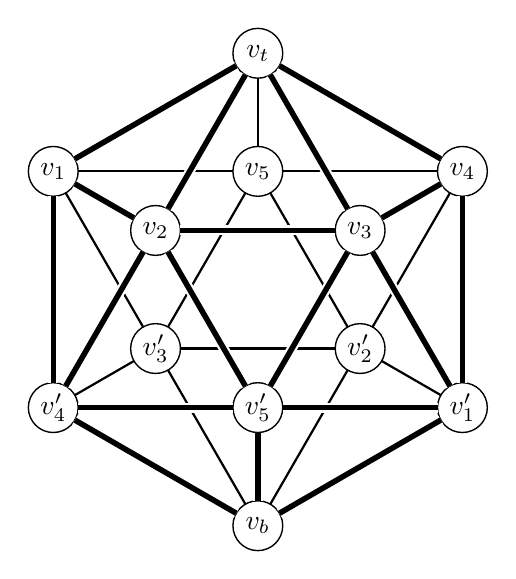
\begin{tikzpicture}
			\begin{scope}[rotate=90]
				\SetVertexNoLabel   % <--- This avoids that default $a_0$, .. $b_0$ labels show up
				\grIcosahedral[form=1,RA=3,RB=1.5]
				
				% Following two lines assign labels to a-like and b-like nodes
				% change it as you prefer
				\AssignVertexLabel{a}{$v_t$, $v_1$, $v_4'$, $v_b$, $v_1'$, $v_4$};
				\AssignVertexLabel{b}{$v_5$, $v_2$, $v_3'$, $v_5'$, $v_2'$, $v_3$};
				
				% The remaining code is unchanged
				\SetUpEdge[color=white,style={double=black,double distance=2pt}]
				\EdgeInGraphLoop{a}{6}
				\EdgeFromOneToSel{a}{b}{0}{1,5}
				\Edges(a2,b1,b3,b5,a4)
				\Edge(a3)(b3)
				\Edges(a1,b1,b5,a5)
				\Edges(a2,b3,a4)
			\end{scope}
		\end{tikzpicture}
	\end{center}

	If $abc$ are three neighboring numbers,
	then $(abc)$ corresponds to the rotation of 60 or 120 degrees along the axis connecting the center of
	faces $(v_t, v_d, v_e)$ and $(v_b,v_d',v_e')$.
	Otherwise, it is the rotation along the axis connecting the center of $(v_a,v_b,v_c)$ and $(v_a',v_b',v_c')$.
	
	There are 10 sets of opposite faces and each set have $C_3$ and $C_3^2$ rotations. In total, it is 20.
	
	\begin{exe}
		\red{TODO}
	\end{exe}

	\begin{def*}[dihedral group]
		The \textbf{dihedral group} $D_{2n}$ is defined to be the group of 
		isometries of a regular $n$-gon in the plane.
	\end{def*}
	\begin{rem*}
		$D_{2n}$ consists of $n$ rotations ($r_0=e,r_1,\dots,r_{n-1}$,
		with $r_i$ meaning counter-clockwise rotation by $\frac{2\pi i}{n}$) and
		$n$ reflections, $s_0,s_1,\dots,s_{n-1}$,
		where the line of symmetry of $s_i$ is rotating $\frac{\pi i}{n}$ counter-clockwise
		from that of $s_0$.
	\end{rem*}
	\begin{rem*}
		If the order of elements denoting the composition is right to left
		(\eg, $s_2s_1$ is the reflection $s_1$ followed by the reflection $s_2$),
		then
		\begin{eqlong}\label{eqD2nMult}
			r_ir_j&=r_{(i+j)\bmod n},\\
			r_is_j&=s_{(i+j)\bmod n},\\
			s_ir_j&=s_{(i-j)\bmod n},\\
			s_is_j&=r_{(i-j)\bmod n}.\\
		\end{eqlong}
		From the multiplication rules, the inverses are
		\begin{eqlong}
			r_i^{-1}&=r_{(-i)\bmod n},\\
			s_i^{-1}&=s_i.\\
		\end{eqlong}
	\end{rem*}
	\begin{prop}
		All rotational operations in $D_{2n}$ form a cyclic (and Abelian) group of order $n$.
	\end{prop}
	\begin{prop}
		The conjugacy classes in $D_{2n}$ are 
		\begin{eqlong}
			\ec{r_i}&=\set{r_{i'}\in D_{2n}|(i-i')\mid n \lor (i+i')\mid n},\\
			\ec{s_i}&=\set{s_{i'}\in D_{2n}| 2\mid(i-i')\lor 2\nmid n}.\\
		\end{eqlong}
	\end{prop}
	\begin{rem*}
		The rotational operation is only conjugate with its inverse.
		All reflections are conjugate if $n$ is odd.
		If $n$ is even, odd-indexed reflections form one conjugacy class and even-indexed ones another.
	\end{rem*}
		
	\begin{proof}
		\[r_jr_ir_{-j}=r_i,s_jr_is_{j}=s_{j}s_{i+j}=r_{-j}.\]
		\[r_js_ir_{-j}=s_{i+j}r_{-j}=s_{i-2j},s_js_is_j=r_{j-i}s_{j}=s_{2j-i}.\]
	\end{proof}
	\begin{exe}
		\red{TODO}
	\end{exe}
	\begin{exe}
		For any $D_{2n}$, there is a trivial representation $U$ corresponding the trivial representation of the cyclic group.
		
		There is another representation $U'$ derived from the same trivial representation of the cyclic subgroup,
		where all reflections are represented as $-1$.
		Easy to show this satisfies group homomorphism from \eqref{eqD2nMult}.
		
		If $n$ is even, there is a alternating representation in the cyclic group ($k=\frac{n}{2}$):
		\[\chi_V(r_j)=\ee^{\frac{2\pi ijk}{n}}=(-1)^{j}.\]
		The representation for reflections could be either
		\[\chi_V(s_i)=(-1)^{i},\]
		or
		\[\chi_{V'}(s_i)=(-1)^{i+1}.\]
		Easy to show this satisfies group homomorphism from \eqref{eqD2nMult}:
		\[\begin{aligned}
			\chi(r_i)\chi(r_j)&=(-1)^{i}(-1)^{j}=(-1)^{i+j}=\chi(r_{i+j}),\\
			\chi(r_i)\chi(s_j)&=(-1)^{i}(-1)^{j+k}=(-1)^{(i+j)+k}=\chi(s_{i+j}),\\
			\chi(s_i)\chi(r_j)&=(-1)^{i+k}(-1)^{j}=(-1)^{i+j+k-2j}=\chi(s_{i-j}),\\
			\chi(s_i)\chi(s_j)&=(-1)^{i+k}(-1)^{j+k}=(-1)^{i+j+2k-2(k+j)}=(-1)^{i-j}=\chi(r_{i-j}).\\
		\end{aligned} \]
		where $\chi$ could be either $\chi_V$ or $\chi_{V'}$ depending on $k$ being 0 or 1.
		
		Such representation does not exist for odd $n$
		because the modulo-$n$ operation does not keep the parity if $n$ is odd.

		For other representations in the cyclic subgroup, $\chi(r_i)=\conj{\chi(r_{-i})}\ne\chi(r_{-i})$.
		Therefore, it must be direct sum of two 1-d representations:
		\[\rho_k(r_j)=\begin{pmatrix}
			\ee^{\frac{2\pi ijk}{n}}&0\\
			0&\ee^{-\frac{2\pi ijk}{n}}\\
		\end{pmatrix}.\]
		The representation for $s_0$ is the second Pauli matrix:
		\[\rho_k(s_0)=\begin{pmatrix}
			0&-i\\
			i&0\\
		\end{pmatrix},
		\]
		which generates representations for other reflections from \eqref{eqD2nMult}:
		\[
		\rho_k(s_j)=\begin{pmatrix}
			0 & -i\ee^{\frac{2\pi ijk}{n}}\\
			i\ee^{-\frac{2\pi ijk}{n}}&0\\
		\end{pmatrix}.
		\]
		Easy to show $\rho_k\colon D_{2n}\to \GL_2(\co)$ is group homomorphism from \eqref{eqD2nMult}.
		Also $\rho_k(r_{n+j})=\rho_k(r_{j}),\rho_k(s_{n+j})=\rho_k(s_{j})$ for all $k\in\inte$.
		
		It can be proved that $(\chi_k,\chi_k)=1$ for $0<k<n/2$.
		
		If $n$ is odd, let $n=2m+1$ where $m\in\nat$. The character table for $D_{2n}$ is
		\begin{center}
			\begin{tabular}{C | C C C C C}
				&1&2&\dots&2&2m+1\\
				&&&&&\\
				D_{4m+2}&e&r_1&\dots&r_m&s_0\\
				\hline
				U&1&1&\dots&1&1\\
				U'&1&1&\dots&1&-1\\
				W_1&2&2\cos\left(\frac{2\pi}{2m+1}\right)&\dots&2\cos\left(\frac{2m\pi}{2m+1}\right)&0\\
				\vdots&\vdots&\vdots&\ddots&\vdots&\vdots\\
				W_k&2&2\cos\left(\frac{2k\pi}{2m+1}\right)&\dots&2\cos\left(\frac{2mk\pi}{2m+1}\right)&0\\
				\vdots&\vdots&\vdots&\ddots&\vdots&\vdots\\
				W_{m}&2&2\cos\left(\frac{2m\pi}{2m+1}\right)&\dots&2\cos\left(\frac{2m^2\pi}{2m+1}\right)&0\\
			\end{tabular}
		\end{center}
		If $n=2m$ where $m\in\inte^{+}$, the character table is
		\begin{center}\label{charTableD4m}
			\begin{tabular}{C | C C C C C C C}
				&1&2&\dots&2&1&m&m\\
				&&&&&&&\\
				D_{4m}&e&r_1&\dots&r_{m-1}&r_m&s_0&s_1\\
				\hline
				U&1&1&\dots&1&1&1&1\\
				U'&1&1&\dots&1&1&-1&-1\\
				V&1&-1&\dots&(-1)^{m-1}&(-1)^m&1&-1\\
				V'&1&-1&\dots&(-1)^{m-1}&(-1)^m&-1&1\\
				W_1&2&2\cos\left(\frac{\pi}{m}\right)&\dots&2\cos\left(\frac{(m-1)\pi}{m}\right)&-2&0&0\\
				\vdots&\vdots&\vdots&\ddots&\vdots&\vdots&\vdots&\vdots\\
				W_k&2&2\cos\left(\frac{k\pi}{m}\right)&\dots&2\cos\left(\frac{(m-1)k\pi}{m}\right)&2\cdot(-1)^k&0&0\\
				\vdots&\vdots&\vdots&\ddots&\vdots&\vdots&\vdots&\vdots\\
				W_{m-1}&2&2\cos\left(\frac{(m-1)\pi}{m}\right)&\dots&2\cos\left(\frac{(m-1)^2\pi}{m}\right)&2\cdot(-1)^{m-1}&0&0\\
			\end{tabular}
		\end{center}
	\end{exe}

	\begin{exe}\label{exe3.9}
		(b)
		Assume $m>0$.
		
		From \ref{thmClCongMat} and \ref{thmEvenCliffAlgComCong}, 
		the following relation is a multiplicative group homomorphism $\rho$ (and another one $\rho'$ if $m$ is even)
		and thus gives a representation $\mathcal{H}=\co^{2^{\ceil{m/2}-1}}$ (and another one $\mathcal{H}'$ if $m$ is even):
		\[
		\begin{aligned}
			H_{2n+1}&\subseteq\Cl_{2n+1}^{[0]}(\co)\cong\Cl_{2n}(\co)\cong\MM_{2^n}(\co)\supseteq \GL(\co^{2^n}),\\
			H_{2n}&\subseteq\Cl_{2n}^{[0]}(\co)\cong\Cl_{2n-1}(\co)\cong\MM_{2^{n-1}}(\co)\oplus\MM_{2^{n-1}}(\co)\supseteq2\GL(\co^{2^{n-1}}),\\
		\end{aligned}
		\]
		where the multiplication by 2 means direct sum.
		
		From \ref{corConjGm0}, we know that elements not in the center are paired as
		$\set{\pm \varepsilon_I}$ in the conjugacy class. Therefore, if $\varepsilon_I\notin \ZZ(H_m)$, then
		(since $\rho$ and $\Tr$ preserve scalar multiplication)
		\[\chi_{\mathcal{H}}(-\varepsilon_I)=\Tr(\rho(-\varepsilon_I))=-\Tr(\rho(\varepsilon_I))=-\chi_{\mathcal{H}}(\varepsilon_I), \]
		but two sides must be equal because $\chi$ is a class function.
		Therefore \[\varepsilon_I\notin \ZZ(H_m)\implies\chi_{\mathcal{H}}(\pm\varepsilon_I)=0.\]
		Similar for $\mathcal{H'}$ if $m$ is even.
		
		We already know from \eqref{eqCoCliffAlgMatRep} that
		\[\chi_{\mathcal{H}}(1)=\chi_{\mathcal{H}'}(1)=\dim \mathcal{H}=2^{\ceil{m/2}-1} .\]
		And from homomorphism:
		\[\chi_{\mathcal{H}}(-1) =\chi_{\mathcal{H}'}(-1)=-\chi_{\mathcal{H}}(1)=-2^{\ceil{m/2}-1} .\]
		
		Therefore, for $m=2n+1$, (rewrite $\mathcal{H}$ as S and $\varepsilon_I$ as $v_I$)
		\begin{center}
			\begin{tabular}{C | C C C C}
				& 1 & 1 & 2 & \dots \\
				\\
				H_{2n+1}& 1 & -1 & \pm v_I & \dots\\
				\hline
				S & 2^n & -2^n & 0 & \dots\\ 
			\end{tabular}
		\end{center}
	
		This is an irreducible representation because 
		\[(\chi_S,\chi_S)=\frac{1}{2^{2n+1}}((2^n)^2+(-2^n)^2)=1.\]
		
		For $m=2n$, the pseudoscalar $\varepsilon_{\inte_m}$ is mapped to the pseudoscalar $\varepsilon_{\inte_{m+1}}$ in $H_{2n+1}(\co)$
		(\red{Can be mapped to $-\varepsilon_{\inte{m+1}}$ as well?}),
		and therefore the representation can be calculated from \eqref{eqCoCliffAlgMatRep}
		(assuming $\rho$ takes the upper left block and $\rho'$ the lower right):
		
		\[\rho(\varepsilon_{\inte_m}) = \left[\prod_{i=1}^{2n}\varphi_{2n}(\bfe_i)\right]i^{n+1}
		\left[\prod_{i=1}^{2n}\varphi_{2n}(\bfe_i)\right]=-(-i)^{n+1}\idm_{2^{n-1}}. \]
		
		Note that $\rho(\bfe_{2n})=i^{n+1}
		\left[\prod_{i=1}^{2n}\varphi_{2n}(\bfe_i)\right]$ and \[i^{n+1}\rho(\varepsilon_{\inte_m})=\rho(\bfe_{2n})\rho(\bfe_{2n})=-\idm_{2^{n-1}}.\]
		
		For lower right block:
		\[\rho'(\varepsilon_{\inte_m}) = \left[\prod_{i=1}^{2n}-\varphi_{2n}(\bfe_i)\right](-i^{n+1})
		\left[\prod_{i=1}^{2n}\varphi_{2n}(\bfe_i)\right]=(-i)^{n+1}\idm_{2^{n-1}}. \]
	
		Therefore we can calculate the character table (as $\rho$ is homomorphism): (take $\rho$ as $S^+$, $\rho'$ as $S^-$,
		$\varepsilon_{\inte_m}$ as $v_{\{1,\dots,2n\}}$ and $\varepsilon_I$ as $v_I$)
		\begin{center}
			\begin{tabular}{C | C C C C C C}
				& 1 & 1 & 1 & 1 & 2 & \dots \\
				\\
				H_{2n}& 1 & -1 & v_{\{1,\dots,2n\}} & -v_{\{1,\dots,2n\}} & \pm v_I & \dots\\
				\hline
				S^+ & 2^{n-1} & -2^{n-1} & (-2i)^{n-1} & -(-2i)^{n-1} & 0&\dots\\ 
				S^- & 2^{n-1} & -2^{n-1} & -(-2i)^{n-1} & (-2i)^{n-1} & 0&\dots\\ 				
			\end{tabular}
		\end{center}
	
		They are irreducible representations because 
		\[(\chi_{S^-},\chi_{S^-})=(\chi_{S^+},\chi_{S^+})=\frac{1}{2^{2n}}(4(2^{n-1})^2)=1.\]
	
		(c)	From \ref{propCenterGm0} and \ref{corConjGm0}, we know that there are
		$2^{2n}+1$ conjugacy classes for $H_{2n+1}$ and $2^{2n-1}+2$ for $H_{2n}$.
		Since the order of $H_m$ is $2\cdot2^{m-1}=2^m$ (\ref{propOrderEvenSubalgebra}),
		all remaining irreducible representations must be one-dimensional %if we find
		because we found
		\begin{itemize}
			\item one $2^n$-dimensional irreducible representation for $H_{2n+1}$,
			\[2^{2n+1}=2^{2n}\cdot 1^2+1\cdot (2^n)^2,\]
			\item two $2^{n-1}$-dimensional irreducible representations for $H_{2n}$,
			\[2^{2n}=2^{2n-1}\cdot 1^2+2\cdot (2^{n-1})^2.\]
		\end{itemize}
		
		Also, the subgroup $\set{\pm1}$ is in the center of $H_m$, and therefore a normal subgroup.
		Therefore, the quotient group $H_m/\set{\pm 1}$ exists.
		It is a Boolean group (elementary Abelian 2-group) isomorphic to a group $\mathcal{G}(H_m)$ of diagonal matrices
		with $\pm1$ diagonal entries and determinant $1$ (\ref{propEvenSubAlgToBool}).
		
		Therefore it has $\card{H_m/\set{\pm 1}}=2^{m-1}$ 1-d irreducible representations which are also 1-d representations in $H_m$
		because elements in the same conjugacy class are mapped to the same element in the quotient subgroup.
		In this way, we have found all irreducible representations of $H_m$.

		Given any subset $A$ of $\inte_{m-1}$ (there are $2^{m-1}$ such subsets), %, see \ref{propOrderEvenSubalgebra}),
		we can construct the character tables (\ref{propChacTblEvenBoolGrp}):
		\begin{center}
			\begin{tabular}{C | C C C C}
				& 1 & 1 & 2 & \dots \\
				\\
				H_{2n+1}& 1 & -1 & \pm v_I & \dots\\
				\hline
				U_A & 1 & 1 & (-1)^{\card{A\cap I}} & \dots \\
				\vdots &\vdots&\vdots&\vdots&\ddots\\
				S & 2^n & -2^n & 0 & \dots\\ 
			\end{tabular}
		\end{center}
		\begin{center}
			\begin{tabular}{C | C C C C C C}
				& 1 & 1 & 1 & 1 & 2 & \dots \\
				\\
				H_{2n}& 1 & -1 & v_{\{1,\dots,2n\}} & -v_{\{1,\dots,2n\}} & \pm v_I & \dots\\
				\hline
				U_A & 1 & 1 &(-1)^{\card{A}}&(-1)^{\card{A}}& (-1)^{\card{A\cap I}} & \dots \\
				\vdots &\vdots&\vdots&\vdots&\vdots&\vdots&\ddots\\
				S^+ & 2^{n-1} & -2^{n-1} & (-2i)^{n-1} & -(-2i)^{n-1} & 0&\dots\\ 
				S^- & 2^{n-1} & -2^{n-1} & -(-2i)^{n-1} & (-2i)^{n-1} & 0&\dots\\ 				
			\end{tabular}
		\end{center}
	
		We see that $U_{\emptyset}$ is the trivial representation.
		
		(a)
		Below are some examples (subscript in concise notation)
		\begin{center}
			\begin{tabular}{C | C C }
				& 1 & 1 \\
				\\
				H_1& 1 & -1 \\
				\hline
				U & 1 & 1 \\
				S & 1 & -1\\ 
			\end{tabular}
		\end{center}
		\begin{center}
			\begin{tabular}{C | C C C C}
				& 1 & 1 & 1 & 1 \\
				\\
				H_{2}& 1 & -1 & v_{\{1,2\}} & -v_{\{1,2\}} \\
				\hline
				U & 1 & 1 &1&1 \\
				U' & 1 & 1 &-1&-1 \\
				S^+ & 1 & -1 & 1 & -1\\ 
				S^- & 1 & -1 & -1 & 1\\ 				
			\end{tabular}
		\end{center}
		\begin{center}\label{charTableH3}
			\begin{tabular}{C | C C C C C }
				& 1 & 1 & 2 & 2 & 2 \\
				\\
				%H_3& 1 & -1 & \pm v_{\{2,3\}}  & \pm v_{\{3,1\}} &  \pm v_{\{1,2\}} \\
				H_3& 1 & -1 & v_{23}  & v_{31} &  v_{12} \\
				\hline
				U & 1 & 1 & 1 & 1 & 1 \\
				U_1 & 1 & 1 & 1 &-1&-1\\
				U_2 & 1 & 1 & -1&1&-1\\
				U_3=U_{12} & 1 & 1 & -1&-1&1\\
				S & 2 & -2 & 0 & 0&0\\ 
			\end{tabular}
		\end{center}
		\begin{center}
			\begin{tabular}{C | C C C C C C C C C C }
				& 1 & 1 & 2 & 2 & 2 &2&2&2&2&2\\
				\\
				H_4& 1 & -1 & v_{1234} & -v_{1234} & v_{12}  & v_{23} &  v_{34} & v_{41} & v_{13} & v_{24} \\
				\hline
				U & 1 & 1 & 1 & 1 & 1 &1&1&1&1&1\\
				U_1 & 1 & 1 &   -1&       -1&          -1&       1     &   1    &   -1     & -1      & 1\\
				U_2 & 1 & 1 & -1&        -1&          -1&       -1    &  1     &  1      & 1      &-1\\
				U_3 & 1 & 1 & -1&        -1&           1&    -1       & -1     & 1       & -1     &1\\
				U_{12}& 1 & 1 &  1&       1&           1&      -1     & 1      &-1       & -1     &-1\\
				U_{23}& 1 & 1 &  1&       1&          -1&       1     &-1      &1        & -1     &-1\\
				U_{123}&1 & 1 & -1&      -1&           1&        1    &    -1  &   -1    &     1  &-1\\
				S^+ & 2 & -2 & -2i & 2i & 0&0&0&0&0&0\\ 
				S^- & 2 & -2 & 2i & -2i & 0&0&0&0&0&0\\ 		
			\end{tabular}
		\end{center}
	
		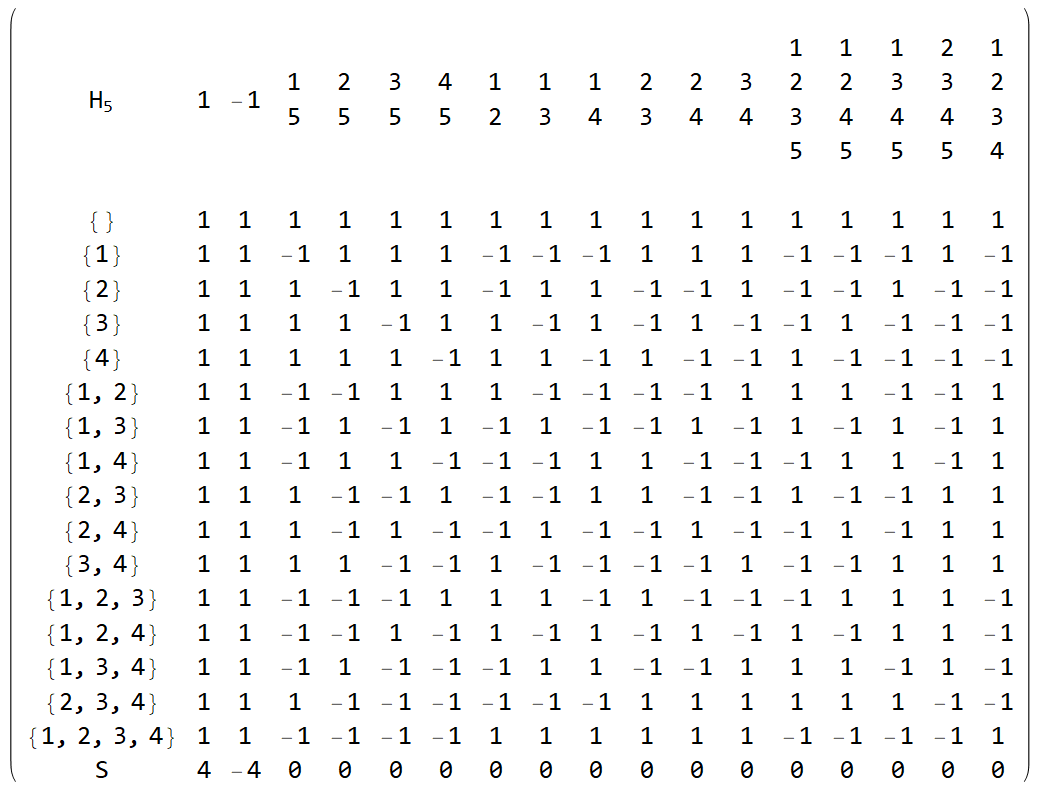
\includegraphics[scale=0.6]{CharacterTable_H5}
		
		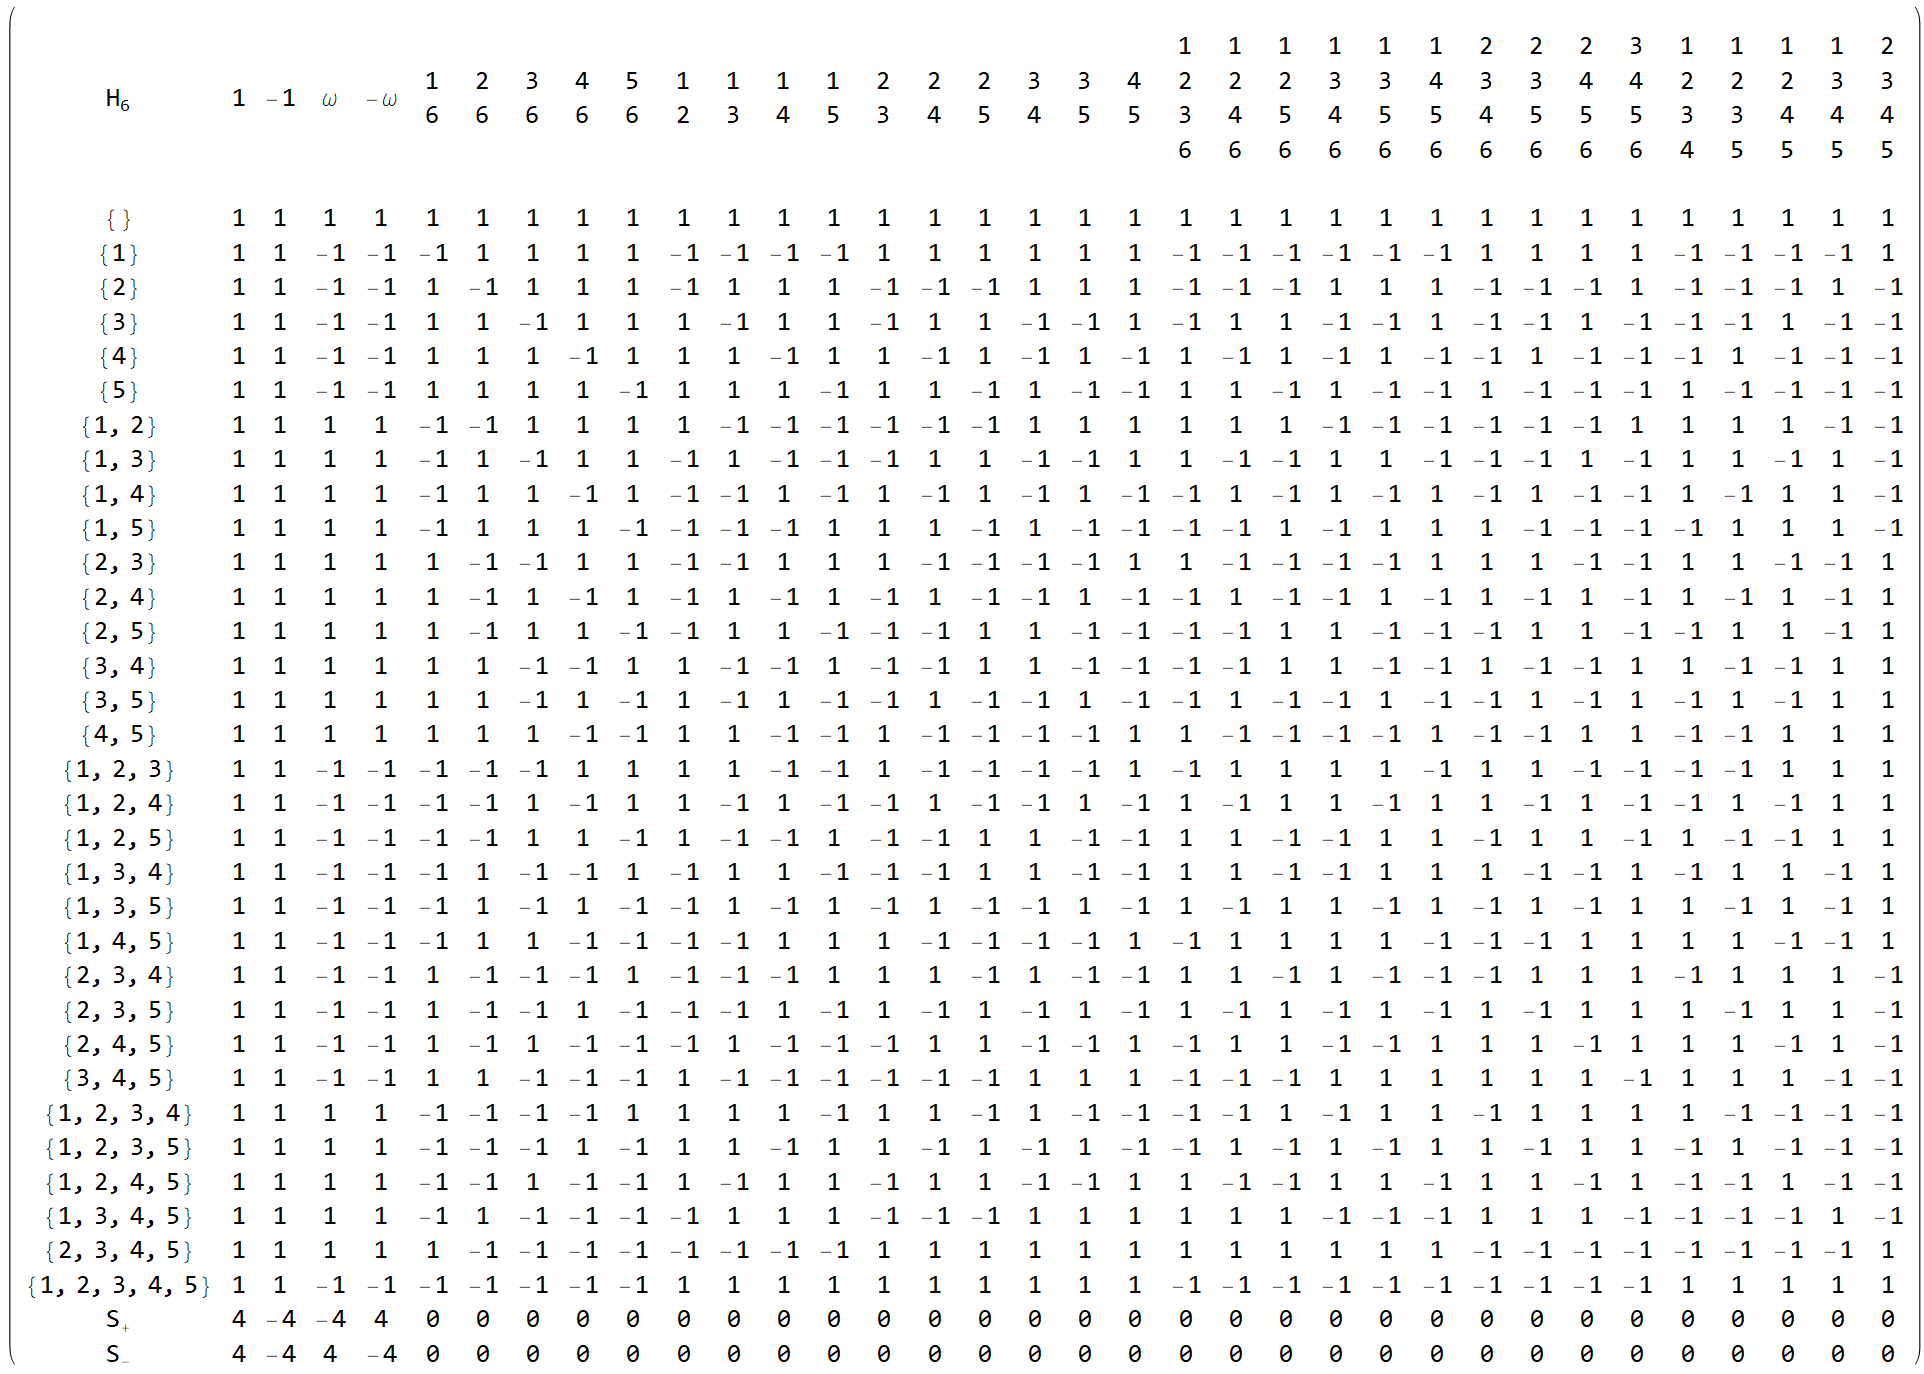
\includegraphics[scale=0.4]{CharacterTable_H6}
	\end{exe}

	\begin{exe}
		\red{TODO}
	\end{exe}
	\begin{exe}
		\red{TODO}
		
		\url{https://people.maths.bris.ac.uk/~matyd/GroupNames/1/He3.html}
	\end{exe}

	\subsubsection{Quadratic Form}
	\begin{def*}[characteristic]
		The \textbf{characteristic} of a ring $R$, often denoted $\operatorname{char}(R)$, is defined to be the smallest number of times one must use the ring's multiplicative identity (1) in a sum to get the additive identity (0). If this sum never reaches the additive identity the ring is said to have characteristic zero.
	\end{def*}
	\begin{rem*}
		Equivalently, $\operatorname{char}(R)$ of a ring $R$ is the smallest positive number $n$ such that
		$\underbrace{1+\cdots+1}_{n \text{ summands}} = 0$
		if such a number $n$ exists, and 0 otherwise.
	\end{rem*}
	\begin{def*}[quadratic form]
		A \textbf{quadratic form}
		$Q\colon V\to K$
		on a vector space $V$ over a field $K$ of arbitrary characteristic is a map from $V$ to $K$ such that
		\begin{itemize}
			\item $Q(a\cdot v) = a^2Q(v), \forall a \in K, v \in V$,
			\item $\Psi\colon V\times V\to K$ defined as $\Psi(u,v)\define Q(u+v)-Q(u)-Q(v)$
			is bilinear.
		\end{itemize}
		$\Psi$ is called the \textbf{bilinear form associated to $Q$}.
	\end{def*}

	\blue{See more in \textit{Quadratic Forms in Infinite Dimensional Vector Spaces} by
		Herbert Gross (1979), pp 354--355.}

	\begin{prop}
		The bilinear form associated to a quadratic form is a
		symmetric form, \ie, $\Psi(u,v)=\Psi(v,u)$.
	\end{prop}
	\begin{proof}
		This is true due to the additive commutativity in $K$ and $V$.
	\end{proof}
	
	\begin{prop}\label{propSymBilToQuad}
		Given a symmetric bilinear form $\Phi\colon V\times V\to K$,
		$Q\colon V\to K$ defined as $v\mapsto\Phi(v,v)$ is a quadratic form.
	\end{prop}
	\begin{proof}
		The first condition holds due to bilinear property of $\Phi$.
		
		The bilinear form $\Psi$ associated to $Q$ is $\Psi(u,v)=\Phi(u+v,u+v)-\Phi(u,u)-\Phi(v,v)=2\Phi(u,v)$
		(the last step is a result of bilinear property and symmetric property of $\Phi$)
		where $2$ is defined as $1+1$ in $K$.
	\end{proof}
	\begin{rem*}
		This is used to construct quadratic form for a commutative ring as well
		(see \url{https://en.wikipedia.org/wiki/Quadratic_form#Generalization}).
	\end{rem*}
	
	\begin{prop}
		For any field of non-2 characteristic,
		there is a unique quadratic form whose associated bilinear form is a given symmetric bilinear form.
	\end{prop}
	\begin{proof}
		Given a symmetric bilinear form $\Psi\colon V\times V\to K$,
		where $V$ is a vector field over field $K$ in which $1+1\ne0$,
		one can construct $Q\colon V\times V\to K$:
		\[
		Q(v)=(1+1)^{-1}\cdot \Psi(v,v).
		\]
		
		From the bilinearity of $\Psi$, we get the first requirement of quadratic form.
		For the second one, consider
		\[
		Q(u+v)-Q(u)-Q(v)=(1+1)^{-1}\cdot [\Psi(u+v,u+v)-\Psi(u,u)-\Psi(v,v)]=\Psi(u,v).
		\]
		Similar to the proof in \ref{propSymBilToQuad}.
		
		If $Q'$ is a quadratic form whose associated bilinear form is $\Psi$,
		then
		\[\Psi(v,v)=Q'(2v)-2Q'(v)=2\cdot(2-1)Q'(v)=2Q'(v),\]
		indicating $Q=Q'$.
	\end{proof}
	\begin{cor}
		If $Q$ is a quadratic form and $\Psi$ is the bilinear form associated to $Q$,
		then
		\[\Psi(v,v)=(1+1)Q(v).\]
	\end{cor}
	\begin{cor}
		For a finite-dimensional vector space over a field of characteristic not 2,
		it suffices to specify the bilinear form on the basis set for uniquely determining
		a quadratic form.
	\end{cor}
	\begin{proof}
		There is always a basis set for a finite dimensional vector field and all elements are
		represented uniquely as the linear combination of bases.
	\end{proof}

	\subsubsection{Clifford Algebra}
	\paragraph{Definition of Clifford algebra}
	\begin{def*}[unital associative algebra]
		Let $R$ be a commutative ring. A \textbf{unital associative $R$-algebra} is a ring that is also an $R$-module
		in such a way that the ring addition and the module addition are the same operation, and scalar multiplication satisfies
		\[r\cdot (xy)=(r\cdot x)y=x(r\cdot y),\]
		for all $r\in R$ and $x, y \in A$.
	\end{def*}
	\begin{rem*}
		A unital associative $R$-algebra $A$ is equipped with three operations:
		\begin{itemize}
			\item ring addition $+\colon A\times A \to A$,
			\item ring multiplication $\cdot\colon A\times A \to A$,
			\item scalar multiplication $\cdot \colon R\times A\to A$.
		\end{itemize}
	\end{rem*}
	\begin{rem*}
		In the definition, the requirement of $R$-module is same as the definition of a vector space.
		
		The distributivity axiom for the ring combined with the compatibility with scalars
		$r\cdot (xy)=(r\cdot x)y=x(r\cdot y)$ consists of additional requirement for an algebra
		(see \url{https://en.wikipedia.org/wiki/Algebra_over_a_field#Definition}).
		
		The algebra being a ring means it is unital (the multiplicative identity of the ring)
		and associative (in terms of ring/algebra multiplication).
	\end{rem*}
	\begin{rem*}\label{remRingAsUniAssAlgebra}
		Equivalently, a \textbf{unital associative algebra} $A$ is a \textit{ring} together with a \textit{ring homomorphism}
		from a commutative ring $R$ to the center of $A$.
	\end{rem*}
	\begin{proof}
		Given a scalar multiplication, one can define such a mapping $\eta\colon R\to A$ as
		\[ \eta(r)=r\cdot I,\]
		where $r\in R$, and $I$ is the multiplicative identity in $A$.
		
		This is a ring homomorphism:
		\[
		\begin{aligned}
			&\text{Distributivity of module multiplication with respect to addition in }R\\
			&\eta(r+s)=(r+s)\cdot I=r\cdot I+s\cdot I=\eta(r)+\eta(s),\\
			&\text{Compatibility of scalar multiplication with multiplication in }R\\
			&\text{Multiplicative identity in }A\\
			&\text{Compatibility of scalar multiplication with multiplication in }A\\
			&\eta(r\cdot s)=(r\cdot s)\cdot I=r\cdot(s\cdot I)=r\cdot(I\cdot(s\cdot I))=(r\cdot I)\cdot(s\cdot I)=\eta(r)\cdot\eta(s),\\
			&\text{Identity element of scalar multiplication}\\
			&\eta(1)=1\cdot I=I,\\
		\end{aligned}
		\]
		where $1\in R$ is the multiplicative identity of $R$.
		
		\[
		\begin{aligned}
			(r\cdot I)\cdot x&=r\cdot(I\cdot x)&\,\text{Identity element of scalar multiplication (left)}\\
			&=r\cdot (x\cdot I)&\,\text{Multiplicative identity in }A\\
			&=x\cdot(r\cdot I),&\,\text{Identity element of scalar multiplication (right)}\\
		\end{aligned}
		\]
		$\forall r \in R, x\in A$.
		Therefore, $\eta(R)\subseteq \ZZ(A)$.
		
		In contrast, given a ring homomorphism $\eta\colon R\to \ZZ(A)$,
		one can define scalar multiplication $\cdot\colon R\to A$ as
		\[r\cdot x = \eta(r) \cdot x,\]
		satisfying all axioms of an $R$-module. For example:
		\[
		\begin{aligned}
			(r\cdot s)\cdot x&=\eta(r\cdot s)\cdot x&\text{Definition of scalar multiplication}\\
			&=(\eta(r)\cdot\eta(s))\cdot x&\text{Ring homomorphism}\\
			&=\eta(r)\cdot(\eta(s)\cdot x)&\text{Multiplicative associativity in }A\\
			&=r\cdot(s\cdot x).&\text{Definition of scalar multiplication}\\
		\end{aligned}
		\]
		Others can be done similarly with ring homomorphism, and distributivity or multiplicative identity in $A$.
		
		The compatibility of scalar multiplication with multiplication in $A$
		requires the property of ring homomorphism, multiplicative associativity in $A$,
		and the fact that $\eta(r)$ commutes with any element in $A$.
	\end{proof}

	\begin{def*}[Clifford algebra]
		Given a vector space $V$ over a field $K$, equipped with a quadratic form $Q \colon V \to K$,
		the \textbf{Clifford algebra} $\Cl(V,Q)$ is the 
		quotient algebra of the tensor algebra $T(V)$
		by the two-sided ideal $I_Q$ generated by all elements of the form
		\[v\otimes v-Q(v)\cdot 1,\forall v\in V,\]
		where $1$ is the multiplicative identity in $T(V)$.
	\end{def*}
	\begin{rem*}
		\begin{eqlong}\label{eqIQ}
			I_Q = \set{\sum_{i=1}^{m}x_i\otimes\left[v_i\otimes v_i-Q(v_i)\cdot 1\right]\otimes y_i
				|m\in \nat,v_i\in V,x_i,y_i\in T(V)	}.
		\end{eqlong}
	\end{rem*}

	\paragraph{Structure of Clifford algebra}
	\begin{prop}
		$\Cl(V,Q)\cong K\oplus V\oplus W$,
		where $W=\bigoplus_{n>1}V^{\otimes n}/I_Q$.
	\end{prop}
	\begin{proof}
		Given any $a,b\in K$, if $a-b\in I_Q$,
		then all terms must have either $x_i$ or $y_i$ being zero,
		otherwise there will be second order term $v_i\otimes v_i$.
		This means $a-b=0$, \ie, every element in $K$ form a equivalent class (as a singleton) in $K/I_Q$.
		
		Similar for $v,u\in V$.
	\end{proof}
	Therefore we can use elements in $K$ and $V$ to represent elements in the subspace of $\Cl(V,Q)$.
	\begin{prop}
		For a finite dimensional vector space $V$ with basis set $(e_i)_{i\in I}$,
		the basis of $\Cl(V,Q)$ is of form
		\[\prod_{i\in I'\subseteq I}e_i=\prod_{i=1}^{\card{I'}}e_{l_i},\]
		given a strict partial order $<$ on $I$,
		\ie, $l_1<l_2<\dots<l_{\card{I'}}$.
		The product evaluates 1 (the multiplicative identity) if $I'=\emptyset$.
	\end{prop}
	\begin{proof}
		We have $\bigotimes_{i=1}^{m}e_i$ as the basis of $T(V)$.
		From \ref{propCliffSqr} and \ref{propCliffAnticomm},
		$e_i\cdot e_j, e_j\cdot c_i, 1$ are linearly dependent,
		and so are $e_i\cdot e_i, 1$.
	\end{proof}

	\begin{prop}
		The dimension of the Clifford algebra on an $n$-dimensional vector space is $2^n$.
	\end{prop}
	\begin{proof}
		There is a bijection from the basis set of the Clifford algebra onto the power set of the basis set of the vector space.
	\end{proof}

	\paragraph{Multiplication in Clifford algebra}
	\begin{prop}\label{propCliffSqr}
		For any $v\in V\subseteq \Cl(V,Q)$,
		$v^2=Q(v)$.
	\end{prop}
	\begin{proof}
		$v^2-Q(v)\in I_Q$.
	\end{proof}
	\begin{prop}\label{propCliffAnticomm}
		The anticommutator in $\Cl(V,Q)$ is given by
		\[[u,v]_{+}=u\cdot v+v\cdot u=\Psi(u,v)\cdot 1,\,\forall u,v\in V, \]
		where $\Psi(u,v)=Q(u+v)-Q(u)-Q(v)$ is the bilinear form associated to $Q$ and $1$ is the multiplicative identity in $\Cl(V,Q)$.
	\end{prop}
	\begin{proof}
		$[u,v]_+=(u+v)^{2}-u^2-v^2=Q(u+v)-Q(u)-Q(v)=\Psi(u,v)$.
	\end{proof}

	\paragraph{Grading}
	\subparagraph{Superalgebra}
	\begin{def*}[graded ring]
		A \textbf{graded ring} is a ring $R$ that is decomposed into a direct sum
		\[R=\bigoplus _{n=0}^{\infty }R_{n}=R_{0}\oplus R_{1}\oplus R_{2}\oplus \cdots \]
		of additive groups $R_0,R_1,\dots$, such that
		$R_{m}R_{n}\subseteq R_{m+n}$
		for all nonnegative integers $m$ and $n$.
	\end{def*}
	\begin{def*}[superalgebra]
		A \textbf{superalgebra} is a $\inte_2$-graded algebra.
		
		Let $R$ be a commutative ring, a \textbf{superalgebra} $A$ over $R$ is an $R$-module
		with direct sum decomposition into two submodules, $A_0$ and $A_1$:
		\[A=A_0\oplus A_1,\]
		together with a bilinear multiplication $A \times A \to A$ such that 
		\[A_iA_j\subseteq A_{i+j},\forall i,j\in\inte_2.\]
	\end{def*}
	\begin{rem*}
		Module + bilinear multiplication are the basic axioms for algebra.
	\end{rem*}
	\begin{def*}[even subalgebra]
		The submodule $A_0$ in above definition forms an ordinary algebra over $R$,
		and thus called a \textbf{even subalgebra}.
	\end{def*}
	\begin{rem*}
		$A_0$ is an algebra because $A_0A_0\subseteq A_{0+0}=A_0$.
	\end{rem*}

	\subparagraph{Division ring}
	\begin{def*}[division ring]
		A \textbf{division ring} is a nonzero ring in which every nonzero element a has a multiplicative inverse.
	\end{def*}
	\begin{rem*}
		A noncommutative division ring is a ``noncommutative field''.
		A commutative division ring is a field.
	\end{rem*}
	\begin{def*}[proper zero divisor]
		Let $(R,+,\cdot)$ be a ring.
		A \textbf{proper (left) zero divisor} of $R$ is an element $x\in R^*$ such that:
		\[\exists y\in R^*[x\cdot y=0],\]
		where $R^*$ is defined as $R\,\setminus \set{0}$.
	\end{def*}
	\begin{prop}
		Division ring has no proper zero divisors.
	\end{prop}
	\begin{proof}
		See \url{https://proofwiki.org/wiki/Division_Ring_has_No_Proper_Zero_Divisors}
		
		By definition of division ring $(R,+,\cdot)$, every element $x \in R^{*}=R\,\setminus\set{0}$ has an element $y$ such that:
		\[y\cdot x=x\cdot y=1.\]
		That is, by definition, every element of $R^*$ is a unit of $R$.
		The result follows from \textit{Unit of Ring is not Zero Divisor}.
	\end{proof}
	\begin{cor}
		If $a,b\in R$ where $R$ is a division ring and $ab=0$,
		then $a=0$ or $b=0$.
	\end{cor}
	\begin{lem}
		If any $a\in R$, where $R$ is a division ring, satisfies $a^2=1$,
		then $a=1$ or $a=-1$.
	\end{lem}
	\begin{proof}
		\begin{eqlong}
			&a^2=1 \iff a^2+a=a+1 &\text{Commutative addition}\\
			&\iff a(a+1)=1(a+1) &\text{Multiplicative identity and distributivity}\\
			&\iff (a-1)(a+1)=0 &\text{Additive inverse and distributivity}\\
		\end{eqlong}
	\end{proof}

	\begin{lem}
		Given a division ring $R$ whose characteristic is not 2,
		$2^{-1}+2^{-1}=1$.
	\end{lem}
	\begin{proof}
		\[2^{-1}+2^{-1}=(1+1)\cdot 2^{-1}=1.\]
	\end{proof}

	\subparagraph{Clifford algebra as superalgebra}
	\begin{lem}
		%Given a division ring $R$ whose characteristic is not 2,
		%an $R$-module $M$,
		%and an involutory module automorphism $f\colon M\to M$,
		%$M$ can be decomposed into eigenspaces of $f$ of eigenvalues $1$ and $-1$.
		Given a field $K$ whose characteristic is not 2,
		a vector space $V$ over $K$,
		and an involutory linear map $f\colon V\to V$,
		$V$ can be decomposed into eigenspaces of $f$ of eigenvalues $1$ and $-1$.
	\end{lem}
	\begin{rem*}
		%This is to say,
		%if $f\in \GL(M)$ and
		%$f\circ f=\idt_M$, then
		%$M=M_1\oplus M_{-1}$,
		%where $M_1$ and $M_{-1}$ are $R$-modules:
		%$M_i=\set{x\in M| f(x)=i\cdot x}$.
		This is to say,
		if $f\in \GL(V)$ and
		$f\circ f=\idt_V$, then
		$V=V_1\oplus V_{-1}$,
		where $V_1$ and $V_{-1}$ are $K$-subspaces:
		$V_i=\set{x\in V| f(x)=i\cdot x}$.
	\end{rem*}

	\begin{proof}
		%Since the characteristic of $R$ is not 2,
		%any $x\in M$ can be decomposed into
		%\[x=g(x)+h(x),\]
		%where $g\colon M\to M$ and $h\colon M\to M$ are endomorphisms
		Since the characteristic of field $K$ is not 2,
		any $x\in V$ can be decomposed into
		\[x=g(x)+h(x),\]
		where $g\colon V\to V$ and $h\colon V\to V$ are endomorphisms
		given by 
		\[\begin{aligned}
			g(x)&=2^{-1}x+2^{-1}f(x),\\
			h(x)&=2^{-1}x-2^{-1}f(x).\\
		\end{aligned}\]
		They are homomorphisms
		\begin{itemize}
			\item for vector addition: because $f$ is automorphism as well as additive commutativity and distributivity of vector space %module
			\item for scalar multiplication: because $f$ is automorphism,
			compatibility of scalar multiplication with field multiplication,
			and commutative multiplication in field.
		\end{itemize}
		\blue{Note that $g(ax)\ne ag(x)$ if $K$ is noncommutative division ring.}
		
		Therefore, the images of $g$ and $h$ are subspaces of $V$:
		\[
		\begin{aligned}
			U&=\operatorname{im}(g)=\set{g(x)\in V|x\in V},\\
			W&=\operatorname{im}(h)=\set{h(x)\in V|x\in V}.\\
		\end{aligned}
		\]
		
		Next, we show they are eigenspaces. As $f$ is involution and homomorphism and vector addition is commutative,
		as well as distributivity in vector space, we have
		\[\begin{aligned}
			f(g(x))&=2^{-1}f(x)+2^{-1}x=g(x),\\
			f(h(x))&=2^{-1}f(x)-2^{-1}x=-h(x),\\
		\end{aligned}
		\]
		indicating $U\subseteq V_1, W\subseteq V_{-1}$.
		
		For any $x\in V_i$, by definition of eigenspace, we have
		\[f(x)=ix,\]
		therefore
		\[2^{-1}x+i2^{-1}f(x)=2^{-1}(1+i^2)x=x,\]
		if $i^2=1$, \ie, $i\in\set{1,-1}$.
		Therefore $U=V_1,W=V_{-1}$.
		
		To conclude the proof, we need to show $U\cap W=\set{0}$.
		If $v,w\in V$ such that $g(v)=h(w)$, then
		\[h(w)=g(v)=f(g(v))=f(h(w))=-h(w),\]
		indicating $2h(w)=0$. Since the characteristic of $K$ is not 2,
		we have $g(v)=h(w)=0$.
	\end{proof}

	\begin{rem*}
		An involution might not be an automorphism. For example, $\alpha \colon \inte_2 \to \inte_2$
		given by
		\[0\mapsto 1, 1\mapsto 0,\]
		is an involution but not automorphism.
	\end{rem*}

	\begin{prop}
		A Clifford algebra over a field of which characteristic is not 2 is a superalgebra.
	\end{prop}
	\begin{proof}
		The linear map on $V$ defined by $v \mapsto -v$ (reflection through the origin)
		preserves the quadratic form $Q$ and so by the \red{universal property} of Clifford algebras
		(the linear map) extends to an algebra automorphism:
		\[\alpha :\Cl (V,Q)\to \Cl (V,Q),\]
		\ie, $\forall v_{ij}\in V$,
		\[
		\begin{aligned}
			&\alpha(\set{x\in T(V)| \left(x - \sum_{j=1}^{k} \bigotimes_{i=1}^{m_j} v_{ij}\right) \in I_Q}) \\
			&=
			\set{x\in T(V)| \left(x - \sum_{j=1}^{k} \bigotimes_{i=1}^{m_j} (-v_{ij})\right) \in I_Q}.\\
		\end{aligned}
		\]
		
		Such $\alpha$ is well-defined bijection because (from \eqref{eqIQ})
		\[
		\begin{aligned}
			&\left[\sum_{j=1}^{k} \bigotimes_{i=1}^{m_j} v_{ij} - \sum_{j=1}^{k'} \bigotimes_{i=1}^{m'_j} v'_{ij}\right]\in I_Q\\
			&\iff \left[\sum_{j=1}^{k} \bigotimes_{i=1}^{m_j} v_{ij} - \sum_{j=1}^{k'} \bigotimes_{i=1}^{m'_j} v'_{ij}\right]
			=\sum_{i=1}^{m}x_i\otimes\left[v_i\otimes v_i-Q(v_i)\cdot 1\right]\otimes y_i\\
			&\iff \left[\sum_{j=1}^{k} \bigotimes_{i=1}^{m_j} (-v_{ij}) - \sum_{j=1}^{k'} \bigotimes_{i=1}^{m'_j} (-v'_{ij})\right]
			=(-1)^2\sum_{i=1}^{m}x'_i\otimes\left[v_i\otimes v_i-Q(v_i)\cdot 1\right]\otimes y'_i\\
			&\iff \left[\sum_{j=1}^{k} \bigotimes_{i=1}^{m_j} (-v_{ij}) - \sum_{j=1}^{k'} \bigotimes_{i=1}^{m'_j} (-v'_{ij})\right]\in I_Q
		\end{aligned}\]
	
		Since $\alpha$ is an involution (\ie, it squares to the identity) one can decompose $\Cl(V, Q)$
		into positive and negative eigenspaces of $\alpha$:
		\begin{eqlong}
			\Cl(V,Q)=\Cl^{[0]}(V,Q)\oplus \Cl^{[1]}(V,Q),
		\end{eqlong}
		where
		\begin{eqlong}
			\Cl^{[i]}(V,Q)=\set{x\in \Cl(V,Q)|\alpha(x)=(-1)^{i}x},\,\forall i \in \inte.
		\end{eqlong}
		Note that $[i]\in \inte_2$.
		
		Given $x\in\Cl^{[i]}(V,Q)$ and $y\in\Cl^{[i]}(V,Q)$,
		since $\alpha$ is homomorphism and the algebra multiplication is compatible with scalar multiplication,
		\[\alpha(xy)=\alpha(x)\alpha(y)=((-1)^{i}x)((-1)^jy)=(-1)^{i+j}(xy). \]
		Therefore, $xy\in\Cl^{[i+j]}(V,Q)$, \ie,
		\[\Cl^{[i]}(V,Q)\Cl^{[j]}(V,Q)\subseteq \Cl^{[i+j]}(V,Q).\]
	\end{proof}

	\begin{prop}\label{propOrderEvenSubalgebra}
		The dimensionality of the even subalgebra of a Clifford algebra $\Cl(V,Q)$ generated by an $n$-dimensional vector space
		$V$ ($n>0$)	is $2^{n-1}$.
	\end{prop}
	\begin{proof}
		By binomial theorem, the dimensionality of the even subalgebra is (because $n>0$)
		\[
		\sum_{k=0}^{\floor{\frac{n}{2}}}\binom{n}{2k}=\frac{1}{2}\left[
		\sum_{i=0}^{n}\binom{n}{i}+\sum_{i=0}^{n}(-1)^i\binom{n}{i}\right]
		=\frac{1}{2}[(1+1)^{n}+(1+(-1))^{n}]=2^{n-1}.
		\]
	\end{proof}

	\subsubsection{Special Clifford Algebras}
	\paragraph{Finite real and complex Clifford algebras}
	Given a field $K$, an $n$-dimensional $K$-vector space $V$,
	with basis set $(e_1,e_2,\dots,e_n)$,
	and the quadratic form $Q\colon V\times V\to K$:
	\[Q\left(\sum_{i=1}^{n}x_ie_i\right)=\sum_{i=1}^{p}x_i^2-\sum_{j=1}^{q}x_{p+j}^2, \]
	the Clifford algebra $\Cl(V,Q)$ is denoted $\Cl_{p,q}(K)$.
	
	\red{Such a (finite) basis set can always be found for $K=\re$ by orthogonal diagonalization as long as $Q$ is nondegenerate.}
	
	If $K=\co$, and $Q$ nondegenerate, then $q$ can always be set to zero by choosing appropriate basis set
	(multiplying by $i$).
	
	See more:
	\url{https://en.wikipedia.org/wiki/Classification_of_Clifford_algebras#Classification}
	
	\url{https://en.wikipedia.org/wiki/Clifford_algebra#Examples:_real_and_complex_Clifford_algebras}
	
	\paragraph{Clifford algebras of negative quadratic form}
	Given a field $K$ of which the characteristic is not 2,
	one can construct a Clifford algebra $C_n=\Cl(V,Q)$,
	where $V=K^n$ is an $n$-dimensional $K$-vector space,
	with basis set $(e_1,e_2,\dots,e_n)$,
	and the quadratic form $Q\colon V\times V\to K$
	is given by its associated bilinear form $\Psi\colon V\times V\to K$,
	\[\Psi(e_i,e_j)=-2\delta_{ij}.\]
	
	\begin{prop}
		$e_i^2=-1,e_ie_j=-e_je_i$ if $i\ne j$.
	\end{prop}
	\begin{prop}
		$\left(\sum_{i=1}^{n}x_ie_i\right)^2=-\sum_{i=1}^nx_i^2$.
	\end{prop}
	\begin{prop}
		$C_n=\Cl_{0,n}(K)$.
	\end{prop}

	\begin{prop}
		$C_0(K)\cong K$.
	\end{prop}

	\begin{prop}
		$C_1(\re)\cong \co$.
	\end{prop}
	\begin{proof}
		$e_1\cong i$.
	\end{proof}
	\begin{prop}
		$C_2(\re)\cong \mathbb{H}$, where $\mathbb{H}$ is the set of quaternions.
	\end{prop}
	\begin{proof}
		$e_1\cong i, e_2\cong j, e_1e_2\cong k$.
	\end{proof}
	\begin{prop}
		\red{$C_3(\re)\cong \mathbb{H}\oplus\mathbb{H}$.}
	\end{prop}
	\begin{proof}
		\red{TODO}
	\end{proof}
	\begin{prop}
		$C_3^{[0]}(\re)\cong \mathbb{H}$.
	\end{prop}
	\begin{proof}
		$1\cong 1, e_2e_3\cong i, e_3e_1\cong j,e_1e_2\cong k$.
	\end{proof}

	See \textit{Linear Algebra and its Applications}
	Volume 128, January 1990, Pages 51--63.
	\textit{Matrix representations of Clifford algebras}
	by Gerald N. Hile and Pertti Lounesto.
	\begin{thm}\label{thmClCongMat}
		\[
		\Cl_{2n}(\co)\cong\MM_{2^n}(\co),
		\Cl_{2n+1}(\co)\cong\MM_{2^n}(\co)\oplus \MM_{2^n}(\co).
		\]
		The isomorphism can be represented
		as the algebra homomorphism $\varphi_m \colon \Cl_{0,m}(\co)\to \MM_{2^{\ceil{m/2}}}(\co)$, which is given recursively:
		(the $\prod$ evaluates 1 if $n=0$)
		\begin{eqlong}\label{eqCoCliffAlgMatRep}
			\varphi_m(1)&=\idm_{2^{\ceil{m/2}}},\\
			\varphi_{2n+1}(\bfe_{j})&=\begin{pmatrix}
				\varphi_{2n}(\bfe_{j})&0\\
				0&-\varphi_{2n}(\bfe_{j})\\
			\end{pmatrix},\forall j\in \inte_{2n},\\
			\varphi_{2n+1}(\bfe_{2n+1})&=i^{n+1}\begin{pmatrix}
				\prod_{j=1}^{2n}\varphi_{2n}(\bfe_{j})&0\\
				0&-\prod_{j=1}^{2n}\varphi_{2n}(\bfe_{j})\\
			\end{pmatrix},\\
			\varphi_{2n+2}(\bfe_{j})&= \varphi_{2n+1}(\bfe_{j}),\forall j \in \inte_{2n+1},\\
			\varphi_{2n+2}(\bfe_{2n+2})&=\begin{pmatrix}
				0&\idm_{2^n}\\
				-\idm_{2^n}&0\\
			\end{pmatrix}.\\
			%\varphi_m(\varepsilon_{\emptyset})&=\idm_{2^{\ceil{m/2}}},\\
			%\varphi_{2n+1}(\varepsilon_{\set{j}})&=\begin{pmatrix}
			%	\varphi_{2n}(\varepsilon_{\set{j}})&0\\
			%	0&-\varphi_{2n}(\varepsilon_{\set{j}})\\
			%\end{pmatrix},\forall j\in \inte_{2n},\\
			%\varphi_{2n+1}(\varepsilon_{\set{2n+1}})&=i^{n+1}\begin{pmatrix}
			%	\prod_{j=1}^{2n}\varphi_{2n}(\varepsilon_{\set{j}})&0\\
			%	0&-\prod_{j=1}^{2n}\varphi_{2n}(\varepsilon_{\set{j}})\\
			%\end{pmatrix},\\
			%\varphi_{2n+2}(\varepsilon_{\set{j}})&= \varphi_{2n+1}(\varepsilon_{\set{j}}),\forall j \in \inte_{2n+1},\\
			%\varphi_{2n+2}(\varepsilon_{\set{2n+2}})&=\begin{pmatrix}
			%	0&\idm_{2^n}\\
			%	-\idm_{2^n}&0\\
			%\end{pmatrix}.\\
		\end{eqlong}
	\end{thm}
	\begin{rem*}
		Easy to show that \[\varphi_{m}(\bfe_{j})\varphi_{m}(\bfe_{j})=-\idm_{2^{\ceil{m/2}}}=\varphi_m(-1),\forall m\in \inte^+,\forall j\in \inte_m.\]
		
		For example,
		\[
		\left[\varphi_{2n+1}(\bfe_{2n+1})\right]^2=(-1)^{n+1}
			\diag (\omega,
			(-1)^2\omega),\]
		where
		\[\begin{aligned}
			\omega&=\prod_{j=1}^{2n}\varphi_{2n}(\bfe_{j})\prod_{j=1}^{2n}\varphi_{2n}(\bfe_{j})\\
			&=(-1)^{n(2n-1)}\prod_{j=1}^{2n}\left[\varphi_{2n}(\bfe_{j})\right]^2\\
			&=(-1)^{n(2n-1)}(-1)^{2n}\idm_{2^n}.\\
		\end{aligned}\]
		Therefore,
		\[\left[\varphi_{2n+1}(\bfe_{2n+1})\right]^2=(-1)^{2n^2+2n+1}
		\idm_{2^{n+1}}=\varphi_{2n+1}(-1).\]
	\end{rem*}
	\begin{rem*}
		Examples:
		\begin{eqlong}
			\varphi_0(1)=\begin{pmatrix}
				1\\
			\end{pmatrix}.\\
			\varphi_1(1)=\begin{pmatrix}
				1&0\\
				0&1\\
			\end{pmatrix},
			\varphi_1(\bfe_1)=\begin{pmatrix}
				i&0\\
				0&-i\\
			\end{pmatrix}.\\
	\end{eqlong}

	%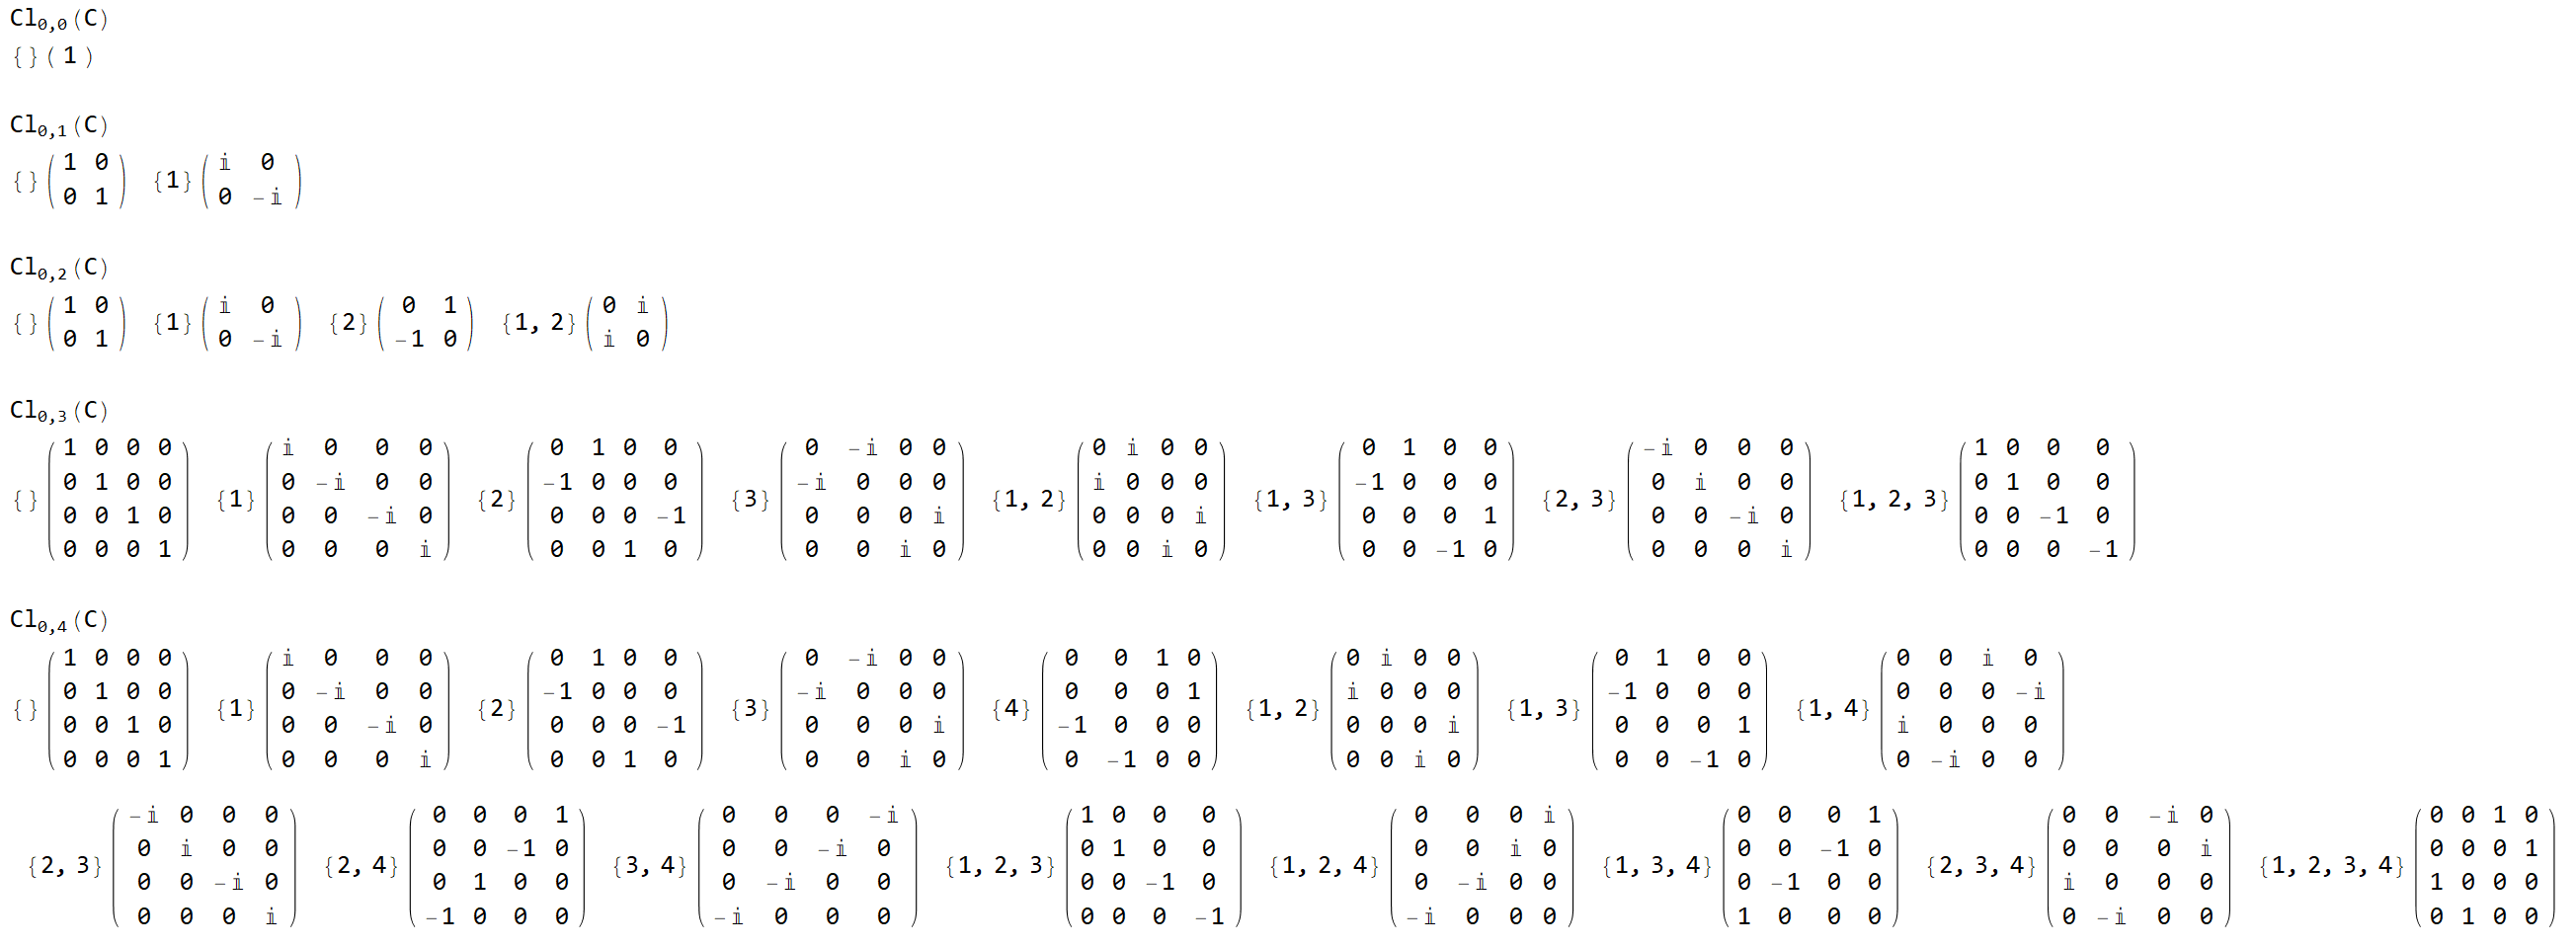
\includegraphics[scale=0.25]{CliffordAlgebraMatrixRepresentation0_4}
	
	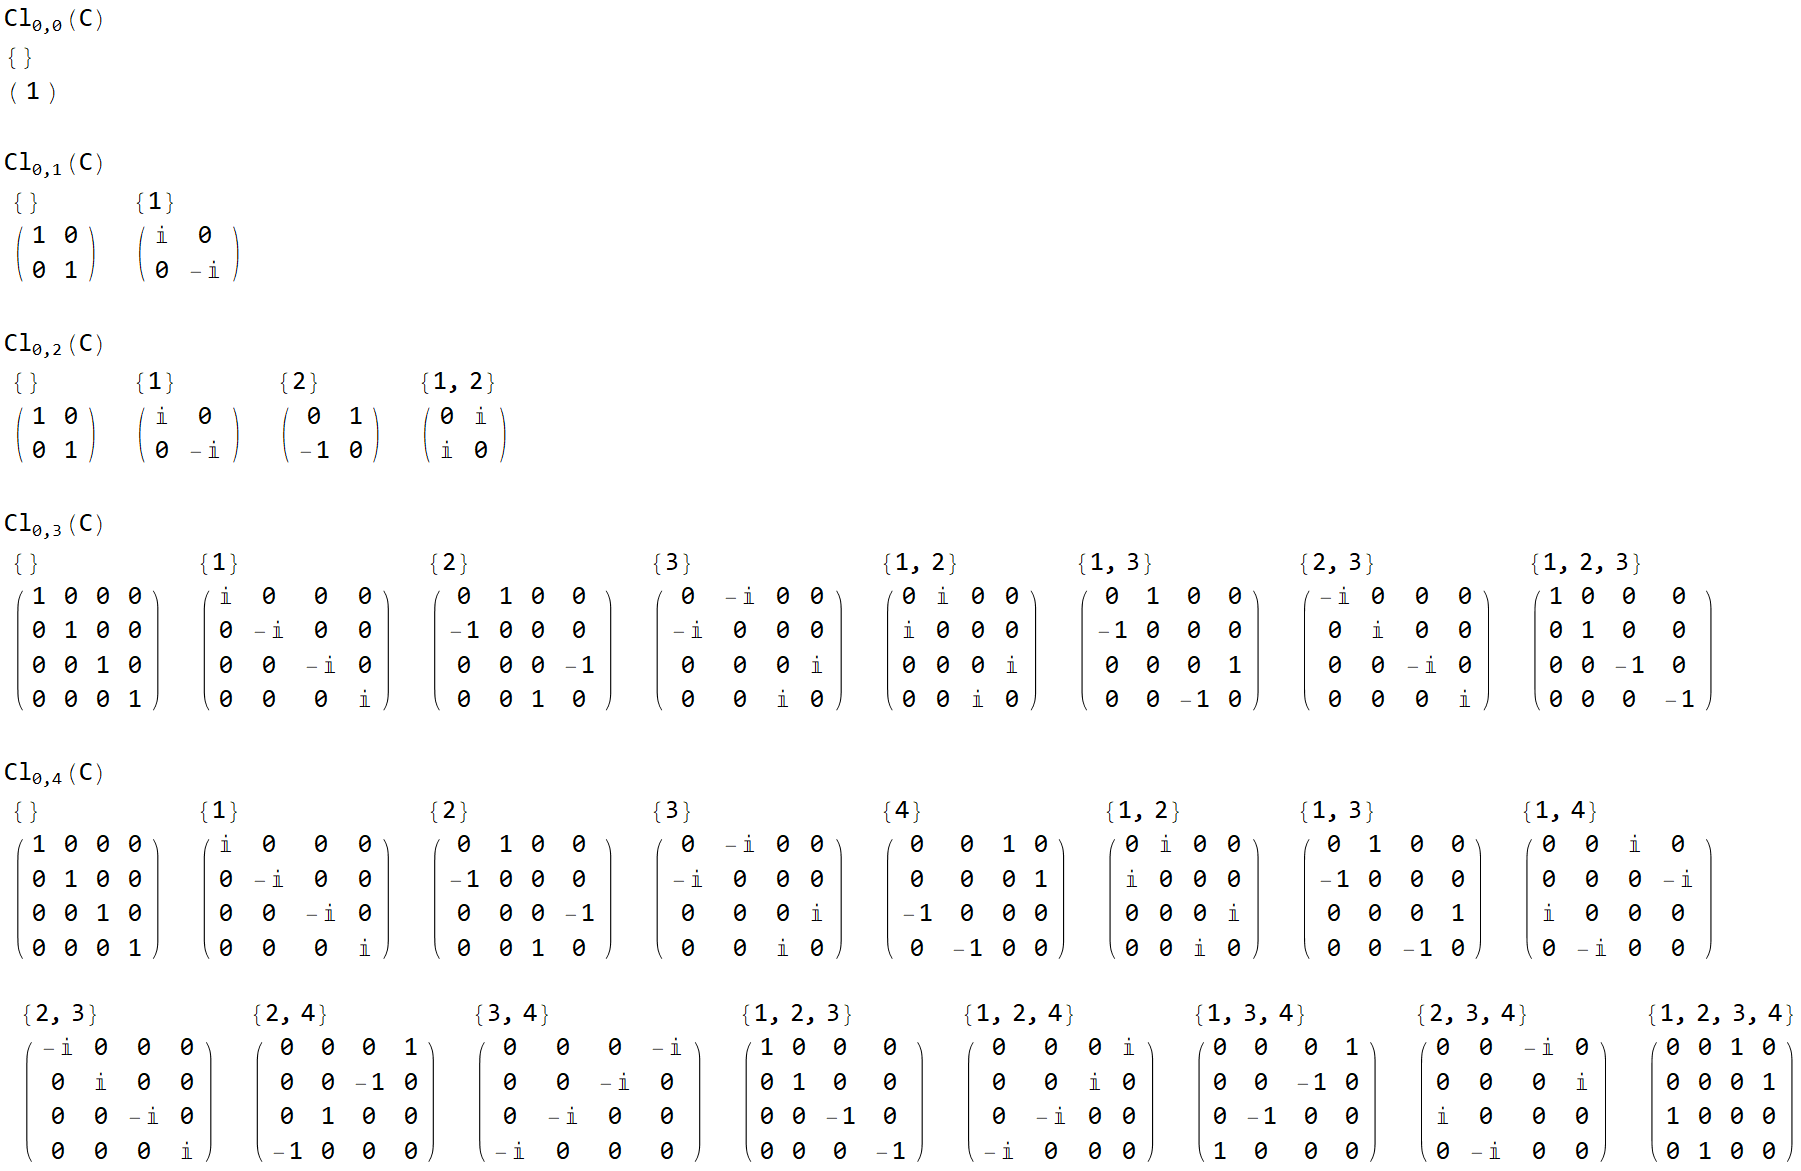
\includegraphics[scale=0.4]{CliffordAlgebraMatrixRepresentationAlt0_4}

	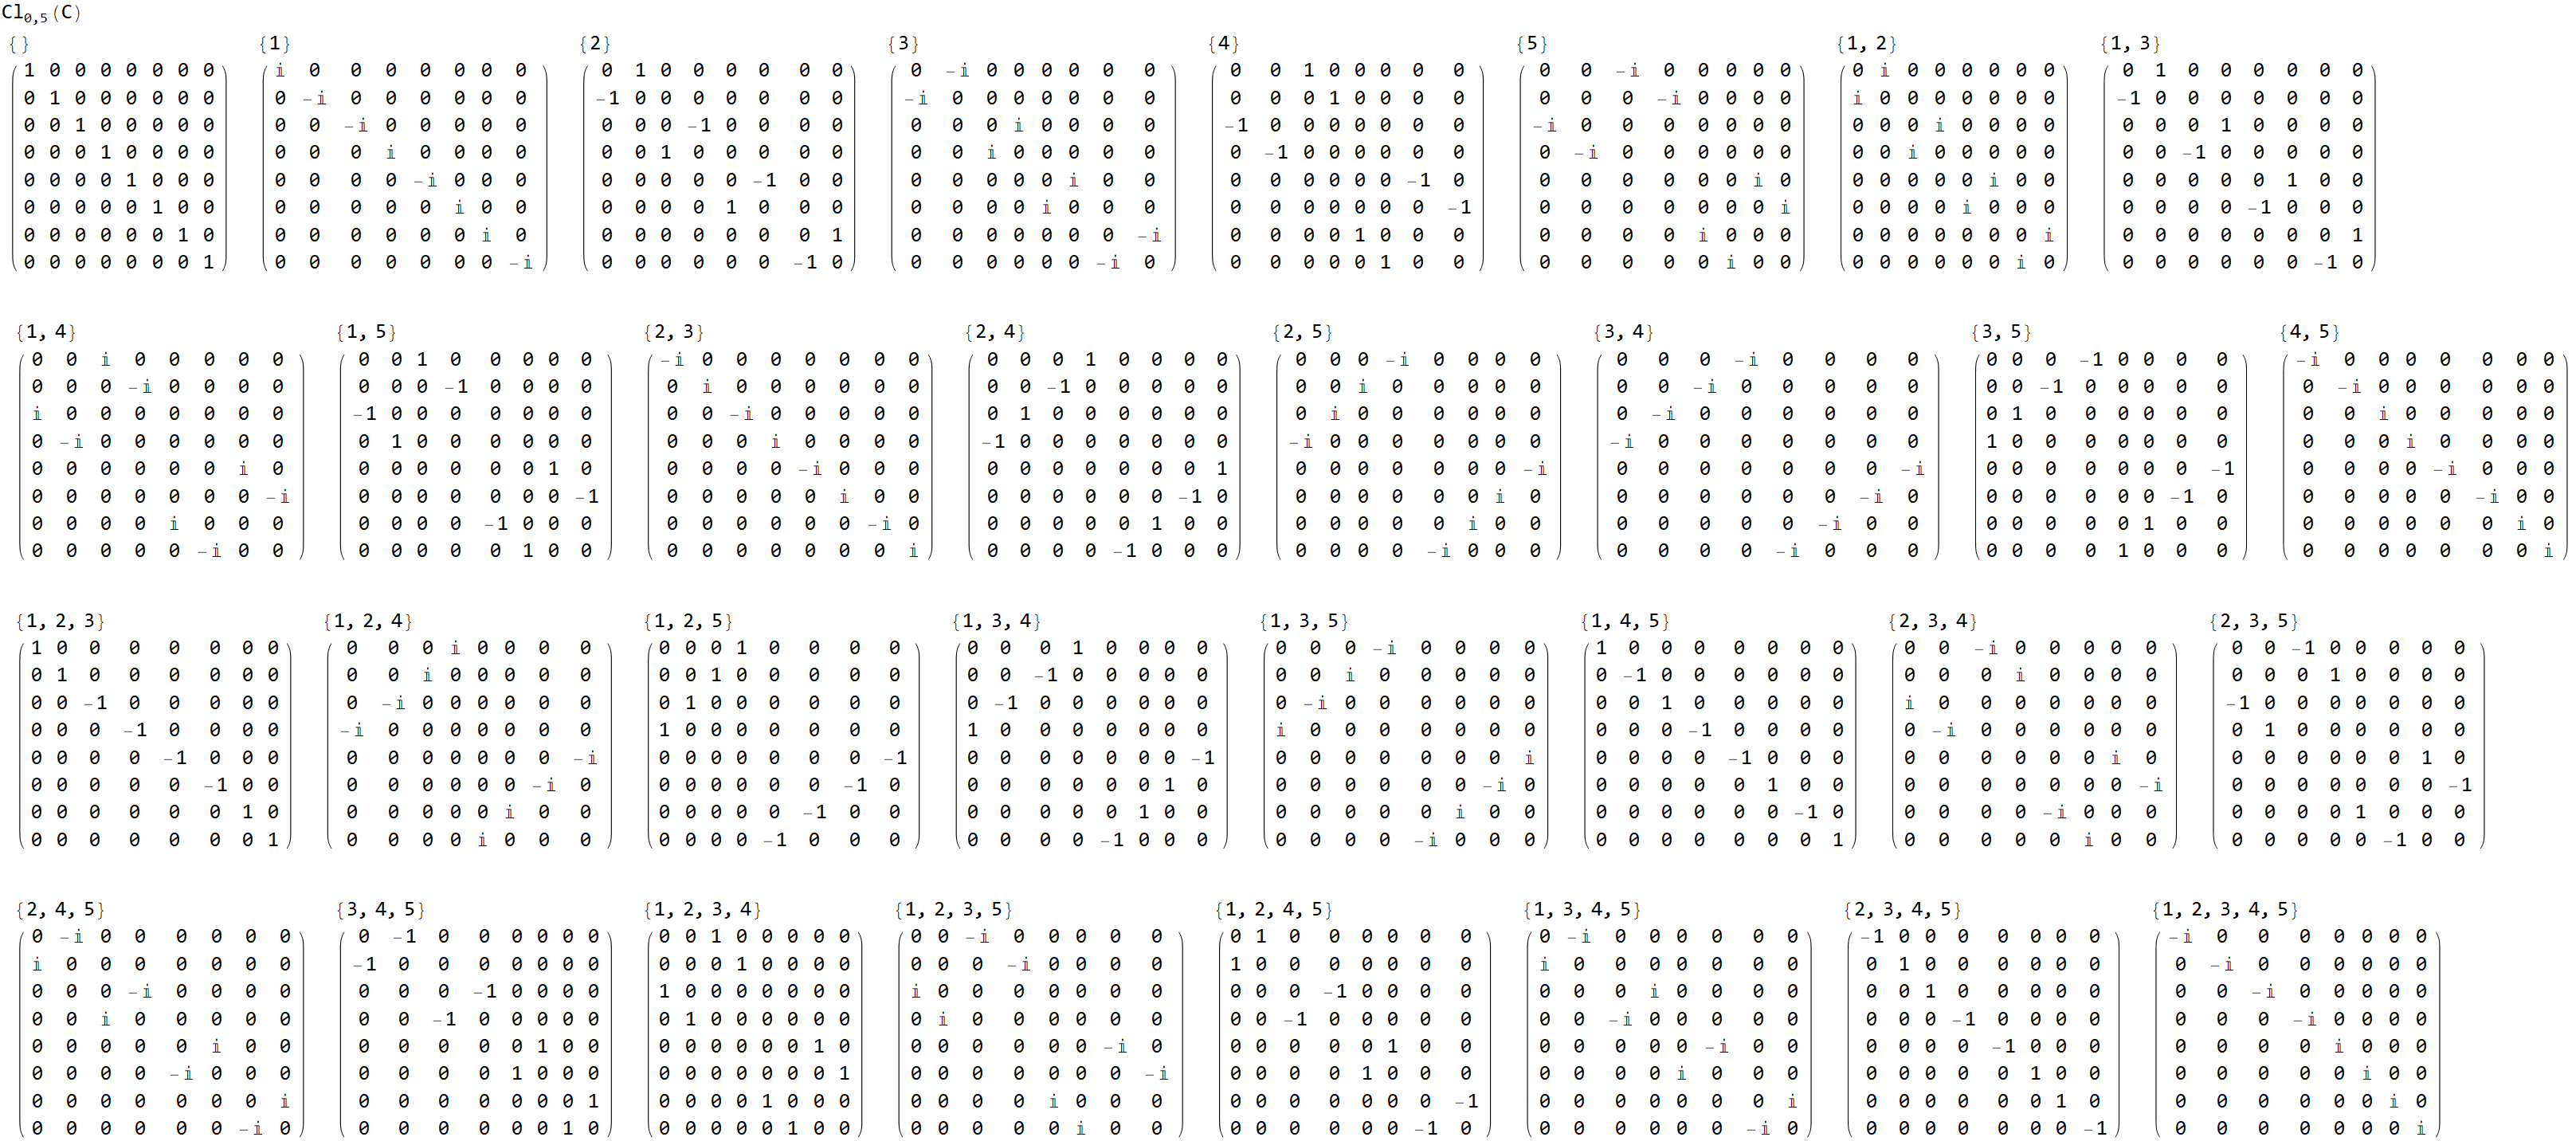
\includegraphics[scale=0.25]{CliffordAlgebraMatrixRepresentationAlt5}
		
	%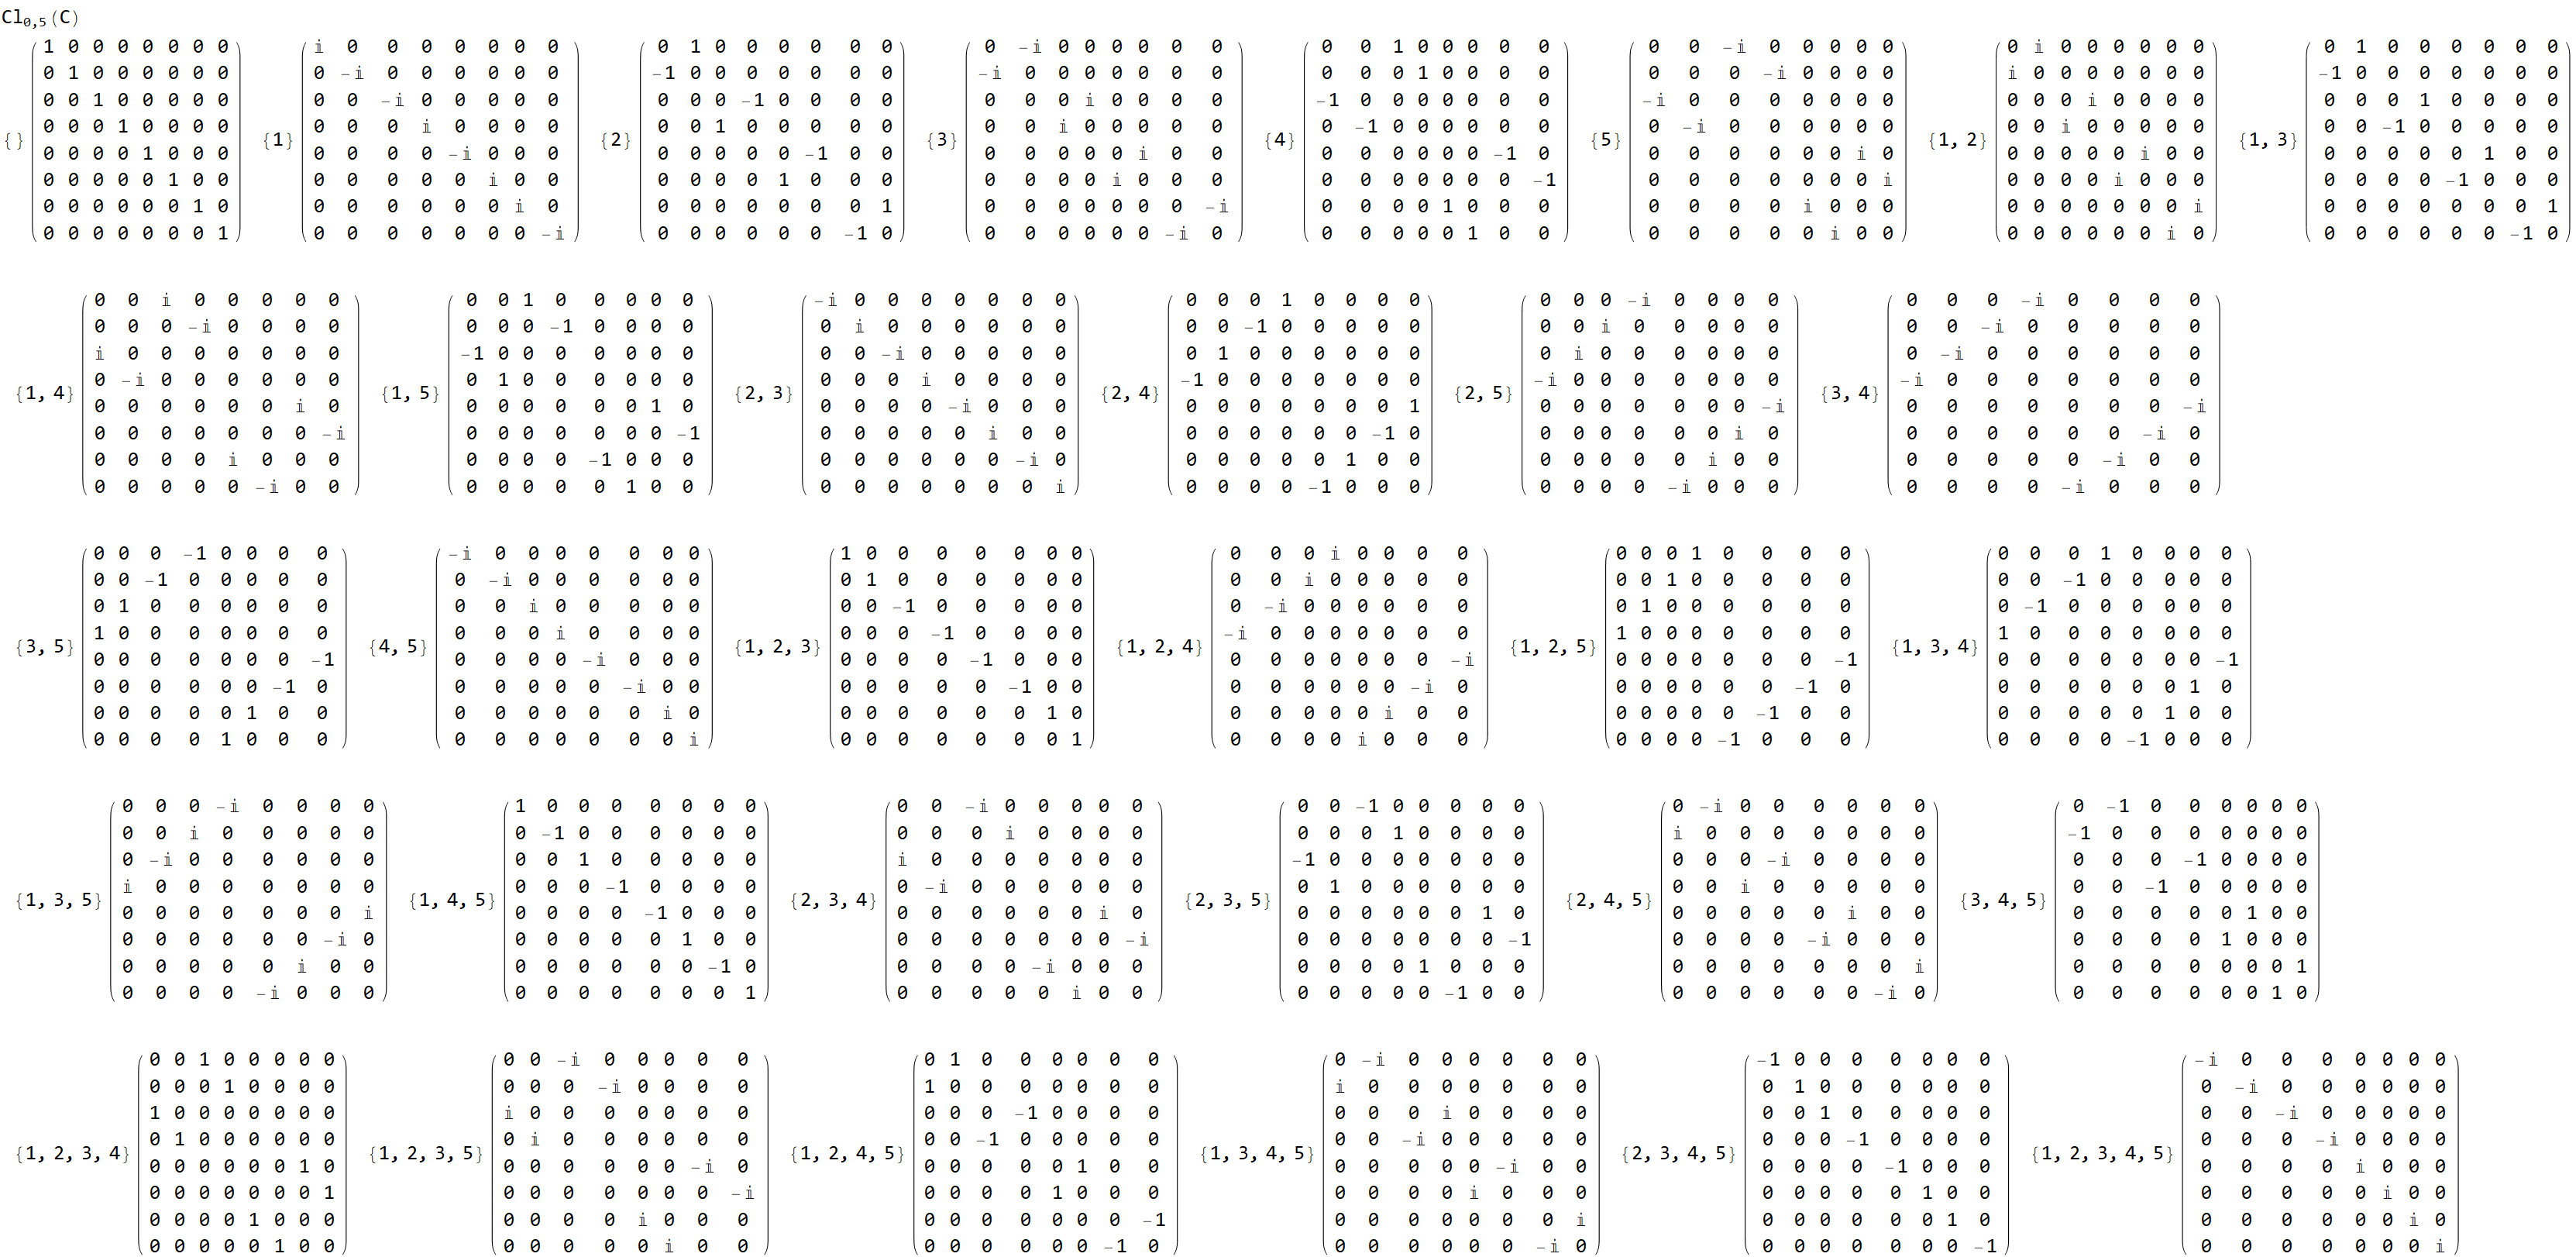
\includegraphics[scale=0.25]{CliffordAlgebraMatrixRepresentation5}

	\end{rem*}

	\red{define real/complex/quaternion/Octonion ($\mathbb{O}$, looks like not)? as even subalgebra}
	
	
	\red{$\Cl_{n+2}(\co)\cong\Cl_n(\co)\otimes\Cl_2(\co)$}
	
	\red{simple ring/ semisimple/ central simple/ Wedderburn--Artin theorem
	}
	
	\red{pin/spin group}

	\red{The even subalgebra $\Cl^{[0]}(V, Q)$ of a Clifford algebra is itself isomorphic to a Clifford algebra.}
	%If V is the orthogonal direct sum of a vector a of nonzero norm Q(a) and a subspace U, then Cl[0](V, Q) is isomorphic to Cl(U, −Q(a)Q), where −Q(a)Q is the form Q restricted to U and multiplied by −Q(a). In particular over the reals this implies that:
	
	\begin{thm}\label{thmEvenCliffAlgComCong}
		\[\Cl_{0,n}^{[0]}(\co)\cong \Cl_{0,n-1}(\co).\]
	\end{thm}
	\begin{proof}
		\red{TODO}
	\end{proof}
	
	%{\displaystyle \operatorname {Cl} _{p,q}^{[0]}(\mathbf {R} )\cong {\begin{cases}\operatorname {Cl} _{p,q-1}(\mathbf {R} )&q>0\\\operatorname {Cl} _{q,p-1}(\mathbf {R} )&p>0\end{cases}}}{\displaystyle \operatorname {Cl} _{p,q}^{[0]}(\mathbf {R} )\cong {\begin{cases}\operatorname {Cl} _{p,q-1}(\mathbf {R} )&q>0\\\operatorname {Cl} _{q,p-1}(\mathbf {R} )&p>0\end{cases}}}
	
	%In the negative-definite case this gives an inclusion Cl0,n−1(R) ⊂ Cl0,n(R), which extends the sequence
	
	%R ⊂ C ⊂ H ⊂ H ⊕ H ⊂ …
	%Likewise, in the complex case, one can show that the even subalgebra of Cln(C) is isomorphic to Cln−1(C).
	
	\subsubsection{Elementary Abelian Group}
	\begin{def*}[p-group]
		Given a prime number $p$, a \textbf{$p$-group} is a group in which the order of every element is a power of $p$.
	\end{def*}
	\begin{def*}[elementary abelian group]
		Given a prime number $p$, an \textbf{elementary abelian group} (or \textbf{elementary abelian $p$-group})
		is an abelian group in which every nontrivial element has order $p$.
	\end{def*}
	\begin{def*}[Boolean group]
		An elementary abelian 2-group is called a \textbf{Boolean group}.
	\end{def*}

	\begin{thm}
		In general, a (possibly infinite) elementary abelian $p$-group is a direct sum of cyclic groups of order $p$.
	\end{thm}

	\url{https://en.wikipedia.org/wiki/Elementary_abelian_group}

	\begin{cor}
		The order of finite elementary abelian $p$-group is power of $p$.
	\end{cor}

	\url{https://proofwiki.org/wiki/Order_of_Boolean_Group_is_Power_of_2}

	\begin{thm}
		Any finite Boolean algebra is isomorphic to the Boolean algebra of the power set of a finite set.
	\end{thm}
	\url{https://en.wikipedia.org/wiki/Power_set#Properties}

	\begin{prop}\label{propChacTblBoolGrp}
		Any finite Boolean group $\inte_2^n\cong\power(\inte_n)$ has the character table, given $A, I\subseteq \inte_n$:
		\begin{center}
			\begin{tabular}{C | C C}
				& 1 & \dots\\
				\\
				\inte_2^n&A&\dots\\
				\hline
				U_I&(-1)^{\card{A\cap I}}&\dots\\
				\vdots&\vdots&\ddots\\
			\end{tabular}
		\end{center}
	\end{prop}
	\begin{proof}
		
		This is a group homomorphism because
		\[\begin{aligned}
			U_I(A)U_I(B)&= (-1)^{\card{A\cap I}}(-1)^{\card{B\cap I}}\\
			&=(-1)^{\card{(A\setminus B)\cap I}+\card{A\cap B\cap I}}
			(-1)^{\card{(B\setminus A)\cap I}+\card{B\cap A\cap I}}\\
			&=(-1)^{\card{(A\setminus B)\cap I}+\card{(B\setminus A)\cap I}}\\
			&=(-1)^{\card{(A\symdif B)\cap I}}\\
			&=U_I(A\symdif B),\\
		\end{aligned}\]
		where $\symdif$ is the symmetric difference, the multiplication in the Boolean group.
		
		There is no repeating representations in the table, \ie,
		\[\forall I,J\subseteq\inte_n \exists A\subseteq\inte_n
		[I\ne J \implies U_I(A)\ne U_J(A)]. \]
		Since $I\ne J$, $I\symdif J$ must be nonempty.
		Let $A$ be the singleton of any element in $I\symdif J$ and the above relation holds.
		
		Since there are $2^{n}$ ways to pick $I$, which is equal to the $\card{\inte_2^n}$,
		the above table is the complete character table.
	\end{proof}

	\begin{prop}\label{propBoolGrpIso}
		The set of all subsets with even cardinality of a finite nonempty set of cardinality $n>0$,
		without loss of generality, $\inte_n$,
		forms a Boolean group under symmetric difference and is isomorphic to $\power(\inte_{n-1})$
		through
		\[A \mapsto A\setminus \set{n}, \]
		where $\set{n}=\inte_n\setminus\inte_{n-1}$.
	\end{prop}
	\begin{proof}
		It is obvious to be a Boolean group.
		
		The map is bijective because any set $B\subseteq\inte_{n-1}$
		can and can only be mapped by $B$ if $\card{B}$ is even or  $B\cup\set{n}$ if $\card{B}$ is odd.

		It is group homomorphism because for any sets $A,B\subseteq\inte_n$,
		we have
		\[ (A\setminus\set{n}) \symdif (B\setminus \set{n}) = (A \symdif B) \setminus \set{n}.\]
	\end{proof}

	\begin{cor}\label{propChacTblEvenBoolGrp}
		The above group has the character table, given $A \subseteq \inte_n$ such that $2\mid\card{A}$,
		and $I\subseteq \inte_{n-1}$:
		\begin{center}
			\begin{tabular}{C | C C}
				& 1 & \dots\\
				\\
				\power^{[0]}(Z_n)&A&\dots\\
				\hline
				U_I&(-1)^{\card{A\cap I}}&\dots\\
				\vdots&\vdots&\ddots\\
			\end{tabular}
		\end{center}
	\end{cor}
	\begin{proof}
		Because \[(A\setminus\set{n})\cap I=A\cap I.\]
	\end{proof}

	\begin{rem*}
		The idea of Boolean group can be generalized into a Boolean algebra.
		
		Consider the subalgebra $B_n$ of diagonal matrices in the matrix algebra $\MM_n(\field_2)$,
		if we assign $0$ to False and $1$ to True, then matrix addition is XOR, while matrix multiplication is AND.
		
		If we instead assign $1$ to False and $0$ to True, then matrix addition is ``=='' or $\iff$,
		and the matrix multiplication is OR.
		
		Similarly, one can construct diagonal matrices with entries in $\set{1,-1}$.
		If we assign $1$ to False and $-1$ to True, then matrix multiplication is XOR,
		element-wise $\max$ is AND, and they form a Boolean algebra as does $B_n$.
		Additionally, element-wise $\min$ is OR.
		
		\textbf{A Boolean algebra generally has two sets of algebra structure.}
		Below is a table of summarizing it.
		\textbf{The identities are parenthesized after the operations.
		The identity of Algebra2 $+$ is always that of Algebra $\times$
		and the identity of Algebra2 $\times$ is always that of Algebra $+$.}
		Note that T is True and F is False.
		\begin{centabular}{c | c c | c c}
			& Algebra $+$ & Algebra $\times$ & Algebra2 $+$ & Algebra2 $\times$\\
			\hline
			$n$-tuples of T/F & XOR $(\text{F}^n$) & AND ($\text{T}^n$) & $\iff$ & OR\\
			Diagonal $\MM_n(\field_2)$ & Mat $+$ ($\mathbf{0}$) & Mat $*$ ($\idm_n$) & Kronecker $\delta$ & $\max$ \\ 
			Diag $\MM_n(\set{1,-1})$ & Mat $*$ ($\idm_n$) & $\max$ ($-\idm_n$) & Mat $-A*B$ & $\min$ \\
			Power set $\power(X)$ & $\symdif$ ($\emptyset$) & $\cap$ (X) & $(A\cap B) \cup (A\cup B)^c$ & $\cup$ \\
		\end{centabular}
	
		Stone's representation theorem for Boolean algebras:
		\textbf{Any Boolean algebra is isomorphic to a subalgebra of some poser set algebra.}
	\end{rem*}

	\subsubsection{Boolean group and Clifford algebra}
	\paragraph{Group homomorphism to Boolean group}
	
	Consider the group homomorphism from a multiplicative group in Clifford algebra to a Boolean group.
	
	Given
	\begin{itemize}
		\item a field $K$ of which the characteristic is not 2  (and denote $K\setminus\{0\}$ as $K^*$),
		\item an $m$-dimensional vector space $V$ over $K$ % ($m>0$)
		with basis $E=\set{\mathbf{e}_1,\mathbf{e}_2,\dots,\mathbf{e}_m}$,% (and denote $V\setminus\{0\}$ as $V^*$),
		\item and a quadratic form $Q\colon V\times V \to K$
		generated by its associated bilinear form
		$(\mathbf{e}_i,\mathbf{e}_j)\mapsto 2a_{i}\delta_{ij}$ where $a_i\in K^*$,
	\end{itemize}
	%elements in $\Cl(V,Q)$ mapped as 	
	%equivalent classes of ``rank-1 elements''
	%nonzero 
	%``pure tensors'' in $T(V)$
	%%, \ie,
	%elements of form
%\[\set{x\in T(V)| (x-\bigotimes_iv_i)\in I_Q} \in \Cl(V,Q) \]
	%given an ordered set of $v_i\in V$, 
%
	%form a multiplicative subgroup of $\Cl(V,Q)$: ($\otimes$ evaluates to 1 if $n=0$)
	%\[\set{\ec{c\bigotimes_{i=1}^nv_i}\in \Cl(V,Q)|c\in K^*, n\in\nat, v_i\in V^*}\subseteq \Cl(V,Q), \]
	%or more explicitly (given the two-sided ideal $I_Q$)
	%\[\set{\set{x\in T(V)| (x-c\bigotimes_{i=1}^nv_i)\in I_Q} \in \Cl(V,Q)|c\in K^*, n\in\nat, v_i\in V^*}, \]
%	
%	the union set of the subspaces spanned by each one of the bases of $\Cl(V,Q)$, excluding $0$,
%	forms a multiplicative subgroup of $\Cl(V,Q)$:
%	\[\set{\ec{c\bigotimes_{i=1}^nv_i}\in \Cl(V,Q)|c\in K^*, n\in\nat, v_i\in E}\subseteq \Cl(V,Q), \]
%	or more explicitly (given the two-sided ideal $I_Q$)
%	\[\set{\set{x\in T(V)| (x-c\bigotimes_{i=1}^nv_i)\in I_Q} \in \Cl(V,Q)|c\in K^*, n\in\nat, v_i\in E}, \]
%	where $\bigotimes$ evaluates to 1 if $n=0$.
%	Its cardinality is $2^{m}(\card{K}-1)$.
%	This is a group because it has
%	
	the union set of the subspaces spanned by each one of the bases of
	% the even subalgebra $\Cl^{[0]}(V,Q)$,
	the Clifford algebra $\Cl(V,Q)$,
	excluding $0$,
	forms a \textit{multiplicative group}:
	\[\set{\ec{c\bigotimes_{i=1}^n\mathbf{v}_i}\in \Cl(V,Q)|c\in K^*, n\in\nat, \mathbf{v}_i\in E}\subseteq \Cl(V,Q), \]
	or more explicitly (given the two-sided ideal $I_Q$)
	\[\set{\set{\lambda \in T(V)| (\lambda-c\bigotimes_{i=1}^n\mathbf{v}_i)\in I_Q} \in \Cl(V,Q)|c\in K^*, n\in\nat, \mathbf{v}_i\in E}, \]
	where $\bigotimes$ evaluates to 1 if $n=0$.
	Its cardinality is $2^{m}(\card{K}-1)$.
	
	\textbf{The group, denoted $G_m$, can be expressed as} (if the algebra multiplication in $\Cl(V,Q)$ is $\cdot$ which can be omitted)
	\[
	G_m = \set{c\prod_{i=1}^k \mathbf{e}_{r_i}|c\in K^*, k\in[0,m]\cap\inte,  1\le r_1<\dots<r_k\le m },
	\]
	where $\prod$ evaluates $1$ if $k=0$.
	Denote $\prod_i\mathbf{e}_{r_i}$ as $\varepsilon_I$ if $I=\set{1\le r_1<\dots<r_k\le m}$
	and $\varepsilon_\emptyset=1$.
	
	This is a group because it has
	%which has
	\begin{itemize}
		\item closed multiplication: as
			\begin{itemize}
				%\item product of nonzero pure tensors is a nonzero pure tensor,
				\item $\mathbf{e}_i^2=a_i\ne0$,
				\item $\mathbf{e}_i\mathbf{e}_j=-\mathbf{e}_j\mathbf{e}_i\ne0$ if $i\ne j$, which is a basis of $\Cl(V,Q)$;
			\end{itemize}
		\item multiplicative associativity: because Clifford algebra is associative;
		\item identity element: since the multiplicative identity $1$ in Clifford algebra is itself a nonzero basis of $\Cl(V,Q)$;% a nonzero pure tensor;
		\item multiplicative inverse: because given any $c\in K^*$ and any ordered index set $I\subseteq \inte_m$
		\[ \left(c\prod_{i\in I}\bfe_i \right)^{-1}=c^{-1}\prod_{i\in I'}a_i^{-1}\bfe_i, \]
		where $I'$ is the reverse of $I$. \\% if $\card{I}$ is even or $I$ itself if $\card{I}$ is odd.
		If the index set is sorted,
		$I=\set{1\le r_1 < r_2 \dots < r_k \le m }$,
		then
		\[\left(c\prod_{i=1}^{k}\bfe_{r_i} \right)^{-1}=c^{-1}\prod_{j=k}^1a_j^{-1}\bfe_{r_{j}}=c^{-1}(-1)^{\frac{k(k-1)}{2}}\prod_{i=1}^ka_i^{-1}\bfe_{r_{i}}, \]
		as a result of $\frac{1}{a_i}\bfe_i\bfe_i=1$.%the square of pure tensors being equivalent to some nonzero scalar (by $I_Q$).
	\end{itemize}
	
	There is a \textbf{group homomorphism} $\mathcal{G}$ from $G_m$ to the group $\GL(m, K)$, which maps
	elements of form 
	\[c\prod_{i=1}^{k}\bfe_{r_i}, \]
	given $c\in K^*,k\in \nat$ and the sorted index set $I=\set{1\le r_1 < r_2 \dots < r_k \le m }$,
	to a diagonal matrix in $\GL(m,K)$ whose main diagonal is $-1$ for $r_i$-th entry and $1$ otherwise.
	
	Easy to show this is a group homomorphism, because if $r_i$-th basis shows up in both multiplicands,
	it disappears in the product, as shown in $\GL(m,K)$ that $(-1)(-1)=1$. Similar for other cases.
	
	The image of $\mathcal{G}$ is a Boolean group and $\card{\operatorname{im}\mathcal{G}}=2^m$.
	
	\paragraph{Commutativity}
	Note that $G_m$ is generally noncommutative.
	
	Given $\alpha, \beta \in G_m$ expressed as
	\[\alpha=c\varepsilon_A, \beta=c'\varepsilon_B,\]
	we consider the relation between $\alpha\beta$ and $\beta\alpha$.
	
	We can always permute $A$ and $B$ while changing signs of $c$ and $c'$ to keep $\alpha$ and $\beta$ unchanged.
	Let all elements in $A\cap B$ be on the right hand side of $\varepsilon_A$ and left hand side of $\varepsilon_B$,
	and align them in reverse order, such that they will disappear directly after multiplication without having to permute,
	then 
	\[\alpha\beta = \left( cc'\prod_{i\in A\cap B}a_i\right) \varepsilon_{A\symdif B},\]
	where $\symdif$ is the ``order-keeping'' symmetric difference.
	
	Now calculate $\beta\alpha$. First, all elements in $A\cap B$ need to be moved from one end to the other end.
	Denote $k=\card{A},l=\card{B},p=\card{A\cap B}$, then the transposition must be done
	\[ \sum_{r=1}^{p}(k-r)+\sum_{r=1}^{p}(l-r) =p(k+l)-p(p+1)\]
	times. Also, when switching from $\varepsilon_{A\symdif B}$ to $\varepsilon_{B\symdif A}$,
	the basis must transpose
	\[\card{A\setminus B}\card{B\setminus A}=(k-p)(l-p)\]
	times.
	Therefore the total transposition is
	\[ pk+pl -p^2-p+kl-pk-pl+p^2=kl-p\]
	times.
	Therefore
	\begin{eqlong}\label{eqCommutGm}
		\beta\alpha=(-1)^{\card{A}\card{B}-\card{A\cap B}}\alpha \beta.
	\end{eqlong}
	
	%with $k$ and $l$ bases in th
	
	\begin{prop}
		The cardinality of any conjugacy class in $G_m$ is at most 2.
	\end{prop}
	\begin{proof}
		Because after swapping the multiplication order, you get either the original product or it multiplied by $-1$.
	\end{proof}
	\begin{cor}
		The conjugacy classes of $G_m$ are singletons $\set{\lambda}$ for $\lambda\in \ZZ(G_m)$
		and $\set{\pm\sigma}$ for $\sigma\notin \ZZ(G_m)$.
	\end{cor}
	
	\paragraph{Center of $G_m$}
	\begin{prop}
		Given any $k\in \nat$,
		\[\begin{aligned}
			\ZZ(G_{2k})&=K^*\\
			\ZZ(G_{2k+1})&=K^{*}\cup\set{c\prod_{i=1}^{2k+1}\bfe_i|c\in K^*}.\\
		\end{aligned}\]
	%\[			\ZZ(G_{2k+1})=\set{c\varepsilon_I\in G_{2k+1}|c\in K^*, I\in\set{\emptyset, \inte_{2k+1}}},\forall k \in \nat,\]
	\end{prop}
	\begin{proof}
		From \eqref{eqCommutGm},
		we know that $\alpha=c\varepsilon_A$ commutes with other elements in the group $G_m$
		if $\card{A}=0$ because $\card{A\cap B}\le \card{A}=0$.
		
		If $\card{A}=m\ne0$ where $m=\dim V$, then $\card{A\cap B}=\card{B}$, so
		\begin{eqlong}\label{eqCommuteFull}
			\beta\alpha=(-1)^{(m-1)\card{B}}\alpha\beta.
		\end{eqlong}
		If $m$ is even, then $m\ge 2$, therefore we can let $\card{B}=1$ such that $\alpha$ does not commute with $\beta$.
		However, if $m$ is odd, then $\alpha$ is in the center.
		
		For $0<\card{A}<m$, we can let $B$ consist of one element of $A$ (because $\card{A}>0$) and one not belonging to $A$
		(which can always be done since $\card{A}<m$), then
		\begin{eqlong}\label{eqCommuteNonFull}
			(-1)^{\card{A}\card{B}-\card{A\cap B}}=(-1)^{\card{A}2-1}=-1\ne1.
		\end{eqlong}
	\end{proof}
	
	\begin{cor}
		\[\ZZ(\Cl(V,Q))=\set{0}\cup \ZZ(G_m).\]
	\end{cor}
	
	\paragraph{Even subalgebra and Boolean group}
	Next, consider the group homomorphism from group in the even subalgebra to a Boolean group.
	
	The subset $G_m^{[0]}$ of $G_m$, constructed as
	\begin{eqlong}
		G_m^{[0]}&=G_m\cap\Cl^{[0]}(V,Q)\\
		&=
		\set{c\prod_{i=1}^k \mathbf{e}_{r_i}|c\in K^*, k\in[0,m]\cap2\inte,  1\le r_1<\dots<r_k\le m },
	\end{eqlong}
	is also a multiplicative group because the multiplication is closed:
	$\mathbf{e}_i^2=a_i\ne0$, meaning the change of number of basis is always even.
	
	\begin{prop}\label{propEvenSubAlgToBool}
		$\mathcal{G}$ is still a group homomorphism. The image are diagonal matrices with $\pm1$ diagonal entries and $+1$ determinant.
	\end{prop}
	
	\begin{prop}\label{propCenterGm0}
		Given any $k\in \nat$,
		\[\begin{aligned}
			\ZZ(G_{2k}^{[0]})&=K^*\cup\set{c\prod_{i=1}^{2k}\bfe_i|c\in K^*},\\
			\ZZ(G_{2k+1}^{[0]})&=K^{*}.\\
		\end{aligned}\]
	\end{prop}
	\begin{proof}
		See \eqref{eqCommuteFull} and \eqref{eqCommuteNonFull}.
		$\card{B}$ is always even in even subalgebra.
		and $\prod_{i=1}^{2k+1}\bfe_i$ is not in the even subalgebra.
	\end{proof}
	\begin{prop}
		The cardinality of any conjugacy class in $G_m^{[0]}$ is at most 2.
	\end{prop}
	\begin{proof}
		Because it is a subgroup of $G_m$.
	\end{proof}
	\begin{cor}\label{corConjGm0}
		The conjugacy classes of $G_m^{[0]}$ are singletons $\set{\lambda}$ for $\lambda\in \ZZ(G_m^{[0]})$
		and $\set{\pm\sigma}$ for $\sigma\notin \ZZ(G_m^{[0]})$.
	\end{cor}
	
	\paragraph{$\Cl_{p,q}$ and Boolean group}
	For $\Cl_{p,q}(K)$, \ie, 
	\[Q\left(\sum_{k=1}^{p+q}z_i\bfe_i\right)=\sum_{i=1}^{p}z_i^2-\sum_{j=1}^{q}z_{p+j}^2,\]
	construct groups
	\[H_{p,q}=\set{c\varepsilon_I\in\Cl_{p,q}(K)|c\in\set{1,-1},I\subseteq \inte_{p+q}},\]
	and
	\[H^{[0]}_{p,q}=H_{p,q}\cap\Cl^{[0]}_{p,q}(K)=\set{c\varepsilon_I\in\Cl^{[0]}_{p,q}(K)|c\in\set{1,-1},I\subseteq \inte_{p+q}}.\]
	
	They are groups because
	\begin{itemize}
		\item $\bfe_i^2\in \set{1,-1}$,
		\item $-1 \in \set{1,-1}$,
		\item $\set{1,-1}$ is a multiplicative group inside $K$.
	\end{itemize}

	$\mathcal{G}$ is still a group homomorphism.
	
	\blue{$H_{0,m}^{[0]}$ is $H_m$ in the book (\ref{exe3.9}). $\mathcal{G}(H_{0,m}^{[0]})$ is the abelian 2-group in the book.}
	
	\subsection{Exterior powers of the standard representation of $\mathfrak{S}_d$}
	\begin{lem}
		For $d>1$, the count for even permutations is equal to that of odd permutations in $\mathfrak{S}_d$.
	\end{lem}
	\begin{proof}
		For any two elements $a, b$ (since $d=\card{X}\ge 2$) in the set $X$ being permuted,
		one can construct a mapping from even permutations to odd permutations
		by transposition of these two elements.

		Any odd permutation has its inverse image by transposition of $a$ and $b$.
		Its inverse image is also unique, and therefore the mapping is bijective. QED.
		%Involution is bijection, QED.
	\end{proof}
	\begin{pprop}
		Exterior power $\ext{k}V$ of standard representation is irreducible.
	\end{pprop}
	\begin{rem*}
		\[\ext{k}\co^d=\bigoplus_{i=0}^{k}\ext{k-i}V\otimes\ext{i}U,\]
		but $\ext{i}U$ are trivial spaces for $i>1$ ($\because\dim U = 1$).
		
		Since $U$ is trivial representation, \ie, all group elements are represented as 1 (multiplicative identity),
		the tensor product of $U$ with any representation does not change the representation.
		
		\red{$\ext{0}W=U$ for any representation $W$?}
		
		For $k=0$, $\ext{k}V=U$ is irreducible. For $k>0$, both $\ext{k}V$ and $\ext{k-1}V$ are not zero representations,
		so $\forall 1\le k\le d-1[(\chi,\chi)=2]\implies$ both of the right hand side are irreducible.
		
		All possible sets $B$ forms the basis for $\ext{k}\co^{d}$. Since $G=\mathfrak{S}_d$ acts on the basis of $\ext{k}\co^d$ as permutation (with possible multiplication by 1), from \ref{exeCharPerm} we know the character for $g\in G$ in $\ext{k}\co^{d}$ is the number of basis fixed by $g$. But even if $g(B)=B$, it might permutes it. As transposition change the sign, all odd permutations should be multiplied by $-1$. Therefore,
		\[\chi(g)=\sum_{g(B)=B} \sgn g|_{B},\]
		where $g|_{B}$ denotes the permutation of the set $B$ determined by $g$.
		
		If $k-l=0$, then $B=C$. If $k-l=1$, then there are
		\[\binom{k}{k-1}\binom{d-k}{1} \]
		ways to choose $C$ given a set $B$. The original equation becomes
		\[\frac{1}{d!} \binom{d}{k} \binom{k}{k-1}\binom{d-k}{1}(k-1)!(d-k-1)!=1. \]
		
		Note that when $k=1$, $\ext{k}V=V$. This is an extension of \ref{propIrrStdRep}.
	\end{rem*}
	\begin{rem*}
		Every irreducible real representation
		admits an inner product (unique, up to scalars) invariant under the group 
		action (corollary from \ref{exe1.14}).
	\end{rem*}

	\subsection{Induced representations}
	\subsubsection{Cosets}
	
	See the definition in \ref{coset}.
	
	\begin{lem}\label{lemgingH}
		Given subgroup $H$ of group $G$ and $g\in G$,
		then \[ g\in gH. \]
	\end{lem}
	\begin{proof}
		The identity $e$ of $G$ is also in $H$,
		therefore $g=ge\in gH$.
	\end{proof}
	
	\begin{lem}\label{lemCosetsCoverAll}
		Given subgroup $H$ of group $G$,
		then the union of all left cosets is the original group $G$.
	\end{lem}
	\begin{proof}
		For any $x\in G$ and there exists a left coset $xH$ 
		containing $x$ because \ref{lemgingH}.
		%xe=x$ where $e$ is the identity in $G$ (and $H$).
	\end{proof}

	\begin{lem}\label{lemCosetToSubGrp}
		Given subgroup $H$ of group $G$ and $g\in G$,
		then \[ g'\in gH\iff g^{-1}g'\in H \iff (g')^{-1}g\in H. \]
	\end{lem}
	\begin{proof}
		\[g'\in gH\iff \exists h\in H[g'=gh] \iff \exists h \in H[g^{-1}g'=h]\iff g^{-1}g'\in H.\]
		The second half holds because any element in $H$ has its inverse
		and $(g^{-1}g')^{-1}=(g')^{-1}g$.
	\end{proof}
	
	\begin{lem}\label{lemSubGrpBijecCoset}
		There is a bijection from the subgroup to any left coset.
	\end{lem}
	\begin{proof}
		Given subgroup $H$ of group $G$ and $g\in G$,
		there is a mapping $\varphi\colon H\to gH$:
		\[\varphi(h)=gh. \]
		
		This is surjective because for any $gh'\in gH$,
		we have $\varphi(h')=gh'$.
		
		This is injective because if $h\ne h'$, but $\varphi(h)=\varphi(h')$,
		then $h=g^{-1}gh=g^{-1}\varphi(h)=g^{-1}\varphi(h')=g^{-1}gh'=h'$, which is contradicting.

	\end{proof}
	
	%\begin{lem}\label{lemSameCoset}
	%	Given subgroup $H$ of group $G$ and a left coset $\sigma$,
	%	then
	%	\[\forall g'\in \sigma[\sigma=g'H]. \]
	%\end{lem}
	%\begin{proof}
	%	%Given a subgroup $H$ of group $G$,
	%	%and $g\in G$.
	%	Let $\sigma$ be $gH$ where $g\in G$.
	%	Then any element $g'$ in the left coset $gH$
	%	can be represented as $\exists h\in H[g'=gh]$.
	%	
	%	Then $g'H = \set{ghh'\in G|h'\in H}$
	%	is a subset of $gH$ because $\forall h'\in H[hh'\in H]$.
	%	
	%	But $gH\subseteq g'H$ because $\forall h' \in H[gh'=gh(h^{-1}h')\in g'H]$.
	%	Therefore $g'\in gH[gH=g'H]$.
	%\end{proof}

	\begin{lem}\label{lemSameCoset}
		Given subgroup $H$ of group $G$, $g\in G$, and a left coset $\sigma$,
		then
		\[g\in \sigma\iff\sigma=gH. \]
	\end{lem}
	\begin{proof}
		$\sigma=gH\implies g\in\sigma$ due to \ref{lemgingH}.
		
		%Given a subgroup $H$ of group $G$,
		%and $g\in G$.
		If $g\in \sigma$, let $\sigma$ be $g'H$ where $g'\in G$,
		\ie, $g\in g'H$.
		Then from \ref{lemCosetToSubGrp}, $(g')^{-1}g\in H$ and $g^{-1}g'\in H$.
		Hence, for any $x\in G$,
		
		\[ \begin{aligned}
			x\in gH \iff& \exists h\in H[x=gh=g'(g')^{-1}gh] \\
			\implies& \exists h \in H\exists h'\in H[x=g'h'\land h'=((g')^{-1}g)h]\\
			\implies &x\in g'H,\\
			x\in g'H\iff& \exists h'\in H[x=g'h'=gg^{-1}g'h'] \\
			\implies& \exists h' \in H\exists h\in H[x=gh\land h=(g^{-1}g')h']\\
			\implies &x\in gH.\\
		\end{aligned}\]
	\end{proof}

	\begin{cor}\label{lemgHg'H}
		Given subgroup $H$ of group $G$ and a left coset $\sigma$,
		then
		\[ \forall g\in G \forall g'\in G [gH=g'H\iff g^{-1}g'\in H\iff (g')^{-1}g\in H].\]
	\end{cor}
	\begin{proof}
		Let $\sigma=gH$ and apply \ref{lemSameCoset}
		\[gH=g'H\iff g'\in gH.\]
		From \ref{lemCosetToSubGrp} we get the second half.
	\end{proof}

	\begin{lem}\label{lemDisjointLeftCoset}
		Different left cosets are disjoint.
	\end{lem}
	\begin{proof}
		Given subgroup $H$ of group $G$ and $g\in G$,
		we have shown in \ref{lemSameCoset} that if $x\in gH$, then $xH=gH$.
		
		For any $x\in G\setminus gH$ (if any),
		if $\exists h,h'\in H[xh=gh']$, then $x=gh'h^{-1}\in gH$ because $h'h^{-1}\in H$.
		This contradicts with $x\notin gH$. Therefore $xH\cap gH=\emptyset$.
		
		Now we have considered all possible cosets, and they are either same cosets or disjoint cosets.
	\end{proof}

	\begin{def*}[quotient set of group over subgroup]
		The \textbf{quotient set} of a group $G$ over its subgroup $H$ is the set of all left cosets:
		\[G/H\define\set{gH\in\power(G)|g\in G}. \]
	\end{def*}

	\begin{prop}\label{lemXsigmaYsigma}
		Given $H$ as a subgroup of a group $G$,
		\[\exists \sigma\in G/H(x\in\sigma \land y\in \sigma)\iff x^{-1}y\in H\iff y^{-1}x\in H.\]
	\end{prop}
	\begin{proof}
		From \ref{lemSameCoset},
		\[\exists \sigma\in G/H(x\in\sigma \land y\in \sigma)\iff \exists \sigma \in G/H(xH=\sigma=yH).\]
		
		Since $xH\in G/H,yH\in G/H$,
		\[\exists \sigma \in G/H(xH=\sigma=yH)\iff xH=yH.\]
		
		With \ref{lemgHg'H}, we finish the proof.
	\end{proof}

	\begin{def*}[left action of group on quotient set]
		Given group $G$ and its subgroup $H$,
		the \textbf{left action of $G$ on $G/H$} is:
		\[g(\sigma) =\set{gg_{\sigma}\in G|g_\sigma\in \sigma}, \]
		for any $\sigma\in G/H$.
		% and $g_\sigma\in\sigma$.
	\end{def*}

	\begin{prop}\label{prop3.53}
		Given subgroup $H$ of group $G$,
		\[\forall g\in G\forall \sigma \in G/H\forall g_\sigma\in\sigma[ g(\sigma)= (gg_{\sigma})H].\]
	\end{prop}
	\begin{proof}
		Since (\ref{lemXsigmaYsigma})
		\[g'_\sigma\in\sigma\land g_\sigma\in\sigma \implies g_\sigma^{-1}g'_\sigma\in H, \]
		and ($g_\sigma H=\sigma$, \ref{lemSameCoset})
		\[ \forall h \in H \exists g'_\sigma=g_\sigma h\in \sigma (g^{-1}_\sigma g'_\sigma=h),\]
		we have
		\[\begin{aligned}
			x\in g(\sigma)\iff &\exists g'_\sigma\in\sigma(gg'_\sigma=x)\\
			\iff& \exists h\in H\exists g'_\sigma\in\sigma(gg_\sigma h=x\land g_\sigma^{-1}g'_\sigma=h)\\
			\iff &\exists h\in H(gg_\sigma h=x)\\
			\iff& x\in(gg_\sigma)H.\\
		\end{aligned}
		\]
		%For any $g'_\sigma\in \sigma$, we have $g'_\sigma H=\sigma=g_\sigma H$ (\ref{lemSameCoset} and $g_\sigma\in\sigma$).
		%From \ref{lemgHg'H}, $g_\sigma^{-1}g'_\sigma\in H$.
		%But \[(gg_\sigma)^{-1}(gg'_\sigma)=g_\sigma^{-1}g^{-1}gg'_\sigma=g_\sigma^{-1}g'_\sigma\in H.\]
		%Therefore $(gg_\sigma) H =(gg'_\sigma) H$ (\ref{lemgHg'H}).
	\end{proof}
	\begin{cor}\label{cor3.54}
		Given subgroup $H$ of group $G$ and $g,g'\in G$,
		\[g(g'H)=(gg')H.\]
	\end{cor}
	\begin{proof}
		we have $g'\in g'H$ (\ref{lemgingH}), from \ref{prop3.53} this is proved.
	\end{proof}
	\begin{cor}\label{lemValidLeftAction}
		The above definition is a valid left action.
	\end{cor}
	\begin{proof}
		For any $g_\sigma\in\sigma$,
		%we have $(g'g_\sigma)\in(g'g_\sigma)H$ (\ref{lemgingH}),
		%therefore
		 from \ref{prop3.53} and \ref{cor3.54}
		\[g(g'(\sigma))=g((g'g_\sigma)H)=(g(g'g_\sigma))H=((gg')g_\sigma)H=(gg')(\sigma).\]
	\end{proof}
	\begin{rem*}\label{rem_g_sigma}
		Since  $g'(g(\sigma))=(g'g)(\sigma)$ (\ref{lemValidLeftAction}),
		and $g(H)=(ge)H=gH$ (since $e\in H$ and \ref{prop3.53})
		there is no ambiguity
		in writing $g(\sigma)$ as $g\sigma$.
	\end{rem*}

	\begin{prop}\label{lemBijectiveAction}
		The left action of a group on the quotient set of the group over its subgroup is a bijection.
	\end{prop}
	\begin{rem*}
		Given group $G$ and its subgroup $H$, any $g\in G$ gives rise to a bijection
		$\alpha(g)\colon G/H\to G/H$.
	\end{rem*}
	\begin{proof}
		Given any $x,y\in G$,
		if $g(xH)=g(yH)$, then 
		$(gx)H=(gy)H$ (\ref{cor3.54}). Therefore $(gy)^{-1}(gx)=y^{-1}x\in H$ (\ref{lemgHg'H}).
		Applying \ref{lemgHg'H} again and we get $xH = yH$. Therefore $g$ is injection.
		
		For any $\sigma\in G/H$, we take $g_\sigma\in\sigma$, 
		$\because g^{-1}g_\sigma\in G,\therefore (g^{-1}g_\sigma)H\in G/H$,
		then (\ref{cor3.54}, \ref{lemSameCoset})
		\[g((g^{-1}g_\sigma)H)= (g(g^{-1}g_\sigma))H=g_\sigma H=\sigma.\]
		Therefore $g$ is a surjection.
	\end{proof}

	\begin{def*}[index]
		The \textbf{index} of a subgroup $H$ in a group $G$ is the number of left cosets of $H$ in $G$,
		denoted $|G:H|$ or $[G:H]$ or $(G:H)$.		
	\end{def*}
	\begin{rem*}
		By definition, it is the cardinality of $G/H$.
	\end{rem*}
	\begin{prop}\label{prop|G|=|G:H||H|}
		 \[|G|=|G:H||H|.\]
	\end{prop}
	\begin{proof}
		Because $G$ is the disjoint union of the left cosets (\ref{lemDisjointLeftCoset}, \ref{lemCosetsCoverAll})
		and because each left coset has the same size as $H$ (\ref{lemSubGrpBijecCoset}),
		the index is related to the orders of the two groups by the formula.
	\end{proof}

	\begin{prop}
		Given a group $G$ and its subgroup $H$,
		the product of two cosets $\rho,\sigma\in G/H$ defined as
		\[\set{xy\in G|x\in\rho ,y\in\sigma},\]
		is a left coset for all $\rho,\sigma\in G/H$ if and only if $H$ is a normal subgroup.
	\end{prop}
	\begin{proof}
		Let $a\in \rho, b\in\sigma$. Then the element in the product set is
		$ahbh'$, where $h,h'\in H$. This is a coset if and only if (\ref{lemXsigmaYsigma})
		\[\forall h_1,h_2,h_3,h_4\in H[(ah_1bh_2)^{-1}(ah_3bh_4)\in H].
		\]
		Let $h_1=h_2=h_4=e$, the identity in $G$ (and $H$), then $b^{-1}h_3b\in H$ is required
		for all $h_3\in H$.
		Since the union of all cosets is $G$ (\ref{lemCosetsCoverAll}),
		this is to say
		\[\forall g \in G [ghg^{-1}\in H],\]
		where $g=b^{-1}$.
		
		If $H$ is a normal subgroup, then \[(ah_1bh_2)^{-1}(ah_3bh_4)=h_2^{-1}(b^{-1}(h_1^{-1}h_3)b)h_4\in H.\]
	\end{proof}
	
	\subsubsection{Main Text}
	\begin{def*}[induced representation]
		Given $H$ as a \textit{subgroup} of group $G$ and representation $V$ of $G$,
		if $W$ as a subspace of $V$ is a \textit{subrepresentation} of $\Res_H^G V$,
		\ie, $\forall h \in H[h(W)=W]$, then
		\[\forall g\in G\forall x \in gH\exists h\in H[x(W) =(gh)(W) =g(h(W))=g(W) ].\]
		Therefore we define $\sigma=gH$ acting on $W$ as
		\[\sigma(W) \define g(W), \]
		%for any $g$ such that $\exists h\in H[gh\in\sigma]$.
		for any $g\in\sigma$.
		Denote the set of all left cosets $\set{gH|g\in G}$ as $G/H$,
		then \textbf{representation} $V$ is \textbf{induced} by $W$ 
		if every element in $V$ can be written \textit{uniquely as a sum} of elements in such 
		translates of $W$, \ie, 
		\[V= \bigoplus_{\sigma\in G/H} \sigma( W).\]
	\end{def*}
	\begin{exam}\label{examPermOnCoset}
		The left action of $G$ on $G/H$ is:
		\[g(\sigma) = (gg_{\sigma})H=\set{gg_{\sigma}h\in G|h\in H}, \]
		where $\sigma=g_{\sigma}H\in G/H$.
		
		Its restriction in $W$ (since $e_H$ is the only basis) is:
		\[h(H)=(h\cdot 1)H=hH=H\implies h(e_H)=e_H, \]
		because $h\in H$ and $H$ has closed multiplication.
		Therefore $W$ is a subrepresentation of $H$.
		It is trivial because $\forall h\in H[h(H)=H]$.
		
		If $\sigma=g_{\sigma}H$, then 
		\[\sigma(W) =g_{\sigma}(W)=\co\cdot e_{g_{\sigma}(1\cdot H)}= \co\cdot e_{\sigma}.\]
		Therefore (since all $\sigma$'s form the basis of $V$)
		\[V=\bigoplus_{\sigma\in G/H}\co\cdot e_{\sigma}=\bigoplus_{\sigma\in G/H}\sigma(W), \]
		which satisfies the definition of induced representation.
	\end{exam}
	
	\begin{exam}
		Given a subgroup $H$ of group $G$, the regular representation $R_H$
		of $H$ is a restriction of $R_G$, \ie,
		\[ R_H(h)(e_{h'})=e_{hh'}=R_G(h)(e_{h'}),\forall h,h'\in H, \]
		and therefore a subrepresentation.
		
		Express $W$ as linear combination of bases:
		\[W=\bigoplus_{h\in H}\co\cdot e_h.\]
		
		If $g_{\sigma}\in\sigma\in G/H$, then
		(the last two equality signs are results of \ref{lemSubGrpBijecCoset} and \ref{lemSameCoset})
		\[\sigma (W) = g_{\sigma} (W)=\bigoplus_{h\in H}\co\cdot e_{g_{\sigma}h}=\bigoplus_{g\in g_\sigma H}\co\cdot e_{g}=\bigoplus_{g\in \sigma}\co\cdot e_{g}.\]
		Then (a result of \ref{lemDisjointLeftCoset} and \ref{lemCosetsCoverAll})
%		\[\bigoplus_{\sigma\in G/H} \sigma (W)= \bigoplus_{\sigma\in G/H}\bigoplus_{h\in H}\co\cdot e_{g_{\sigma}h}. \]
		\[\bigoplus_{\sigma\in G/H} \sigma (W)= \bigoplus_{\sigma\in G/H}\bigoplus_{g\in \sigma}\co\cdot e_{g}=\bigoplus_{g\in G}
		\co\cdot e_g=V. \]
		Therefore, $V$ is induced by $W$.
		%If $gh=g'h'$, they must be in the same $\sigma$ (because left cosets are equivalence classes),
		%\ie, $gH=g'H=\sigma$,
		%and therefore not be added twice (because for a specific $\sigma$, $h\ne h'\implies g_{\sigma}h\ne g_{\sigma}h'$).
		%
		%Such $g_{\sigma} h$ will cover all elements in $G$ because $\sigma$ is enumerated over $G/H$.
		%For any $x\in G$ and $h\in H$, there exists $\sigma = (xh^{-1})H\in G/H$ (because $xh^{-1}\in G$)
		%such that $x=(xh^{-1})h=g_{\sigma}h\in\sigma$.
		%\red{TODO}
		%
		%Therefore,
		%\[ \bigoplus_{ \sigma\in G/H}\bigoplus_{h\in H}\co\cdot e_{g_{\sigma}h} = V,\]
		%and $V$ is induced by $W$.
	\end{exam}
	
	\begin{prop}
		Given a representation $W$ of $H$ as a subgroup of $G$, the induced representation $V$ exists and is unique 
		up to isomorphism.
	\end{prop}
	\begin{proof}
		Given a subgroup $H$ of group $G$
		and a representation of $H$: $(W,\rho_W\colon H\to\GL(W))$,
		we can define copies of $W$ by introducing isomorphisms
		\[I_H^\sigma(W)=W^{\sigma}\] for each $\sigma\in G/H$, with $I_H^H$ being the identity map,
		\ie, \begin{eqlong}\label{eqIHHidm}
			W^H&=W,\\ I_H^H(w)&=w,\forall w\in W.\\
		\end{eqlong}
		
		Easy to show composites $I_{\sigma'}^{\sigma}= I_{H}^{\sigma}\circ\left( I_{H}^{\sigma'}\right)^{-1}$ are also isomorphisms.
		%And they form a group under composition.
		It is easy to show that
		the inverse function is given by $\left( I_{\sigma'}^{\sigma}\right)^{-1} =I_{\sigma}^{\sigma'}$.
		
		Then the vector space $V$ over the same field can be constructed as
		\[V=\bigoplus_{\sigma\in G/H}W^{\sigma},\]
		and define $P^{\sigma}\colon V\to W^{\sigma}$ as the projection from $V$ onto $W^\sigma$,
		and the injection $I_{\sigma}\colon W^{\sigma}\to V$.
				
		Next we define 
		%the map $\lambda\colon G\to G/H$ such that
		%\[g\in\lambda(g).\]
		%This can be uniquely defined as a result of \ref{lemDisjointLeftCoset} and \ref{lemCosetsCoverAll}.
		%We then define
		 some $\varphi \colon G/H \to G$ such that
		\begin{eqlong}\label{eqVarphiSigma}
		\varphi(\sigma)\define
		\begin{cases} 
			e & \sigma=H \\
			g_\sigma\in\sigma & \sigma\ne H \\
		\end{cases},
		\end{eqlong}
		where $e$ is the identity in $G$ (and $H$).
		There might be multiple ways to define $\varphi$ by picking different $g_\sigma$ for each coset $\sigma\in G/H$,
		but we will show they generate isomorphic representations.
		Now we choose them arbitrarily and fix it in the following discussion.
		
		$\because e\in H,\therefore \varphi(\sigma)\in\sigma$.
		As a result of (\ref{lemSameCoset}),
		\begin{eqlong}\label{eqVarphiSigmaH}
			\varphi(\sigma) H =\sigma.
		\end{eqlong}
		
		Given $\varphi$, 
		we \textbf{define} $\rho_V\colon G\to \GL(V)$ such that for all $g\in G$
		($\rho_V(g)$ is a linear map because all components are linear maps),
		\[\rho_V(g) =\sum_{\sigma\in G/H} I_{\tau_\sigma}\circ I_{H}^{\tau_\sigma}\circ \rho_W(h_\sigma)\circ I^{H}_{\sigma}\circ P^\sigma, \]
		where
		\[\begin{aligned}
			%\tau_\sigma&=\lambda(g\varphi(\sigma))\in G/H,\\
			\tau_\sigma&=(g\varphi(\sigma))H\in G/H,\\
			h_\sigma&=(\varphi(\tau_{\sigma}))^{-1}g\varphi(\sigma)\in H.\\
		\end{aligned} \]
		$h_\sigma\in H$ because $g\varphi(\sigma)\in\tau_\sigma$ (\ref{lemgingH}) and $\tau_\sigma =\varphi(\tau_\sigma)H$
		(\eqref{eqVarphiSigmaH}) and \ref{lemCosetToSubGrp}.
		Therefore $\rho_W(h_\sigma)$ is well-defined.

		We then show $\rho_V$ is a \textbf{group homomorphism}.
		
		Since $\tau_\sigma=(g\varphi(\sigma))H=g(\varphi(\sigma)H)=g(\sigma)$ is an action (\ref{cor3.54}, \eqref{eqVarphiSigmaH}),
		for a given $g\in G$, the map $\sigma\mapsto\tau_{\sigma}$ is a
		bijection $G/H\to G/H$.
		
		Therefore we can rewrite (use $\varphi_\sigma$ as a short notation of $\varphi(\sigma)$ and $g\sigma$ for $g(\sigma)$ (\ref{rem_g_sigma})):
		\begin{eqlong}\label{eqIndRep}
			h_\sigma&=\varphi_{g\sigma}^{-1}g\varphi_{\sigma},\\
			\rho_V(g)&=\sum_{\sigma\in G/H} I_{g\sigma}\circ I_{H}^{g\sigma}\circ \rho_W(\varphi_{g\sigma}^{-1}g\varphi_{\sigma})\circ I^{H}_{\sigma}\circ P^\sigma.\\
		\end{eqlong}

		\begin{centikzcd}\label{diagSigmaWToGSigmaW}
			V\ar[r,"P^\sigma"]&W^\sigma\ar[r,"I_\sigma^H"]&W\ar[rr,"\rho_W(\varphi_{g\sigma}^{-1}g\varphi_{\sigma})"]&&W
			\ar[r,"I_H^{g\sigma}"]&W^{g\sigma}\ar[r,"I_{g\sigma}"]&V\\
		\end{centikzcd}

		Since $P$ is projection, we have
		\[ I^{H}_{\sigma'}\circ P^{\sigma'}\circ I_{\sigma}\circ I_{H}^{\sigma}=\idt_W \delta_{\sigma\sigma'}. \]
		
		Therefore (bijection + projection),
		\[\begin{aligned}
			\rho_V(g')\rho_V(g)=&\sum_{\sigma'\in G/H} I_{g'\sigma'}\circ I_{H}^{g'\sigma'}\circ \rho_W(h'_{\sigma'})\circ I^{H}_{\sigma'}\circ P^{\sigma'}\\
			&\sum_{\sigma\in G/H} I_{g\sigma}\circ I_{H}^{g\sigma}\circ \rho_W(h_\sigma)\circ I^{H}_{\sigma}\circ P^\sigma\\
			=&\sum_{\sigma\in G/H} I_{g'g\sigma}\circ I_{H}^{g'g\sigma}\circ \rho_W(h'_{g\sigma})\circ \rho_W(h_\sigma)\circ I^{H}_{\sigma}\circ P^\sigma.\\
		\end{aligned}\]
	%	\[\begin{aligned}
	%		\rho_V(g')\rho_V(g)=&\sum_{\sigma'\in G/H} I_{g'(\sigma')}\circ I_{H}^{g'(\sigma')}\circ \rho_W(h'_{\sigma'})\circ I^{H}_{\sigma'}\circ P^{\sigma'}\\
	%		&\sum_{\sigma\in G/H} I_{g(\sigma)}\circ I_{H}^{g(\sigma)}\circ \rho_W(h_\sigma)\circ I^{H}_{\sigma}\circ P^\sigma\\
	%		=&\sum_{\sigma\in G/H} I_{g'(g(\sigma))}\circ I_{H}^{g'(g(\sigma))}\circ \rho_W(h'_{g(\sigma)})\circ \rho_W(h_\sigma)\circ I^{H}_{\sigma}\circ P^\sigma.\\
	%	\end{aligned}\]
	
		Since $\rho_W$ is a group homomorphism (also \eqref{eqIndRep}),
		\[ \rho_W(h'_{g\sigma})\circ \rho_W(h_\sigma)= \rho_W(\varphi_{g'g\sigma}^{-1}g'\varphi_{g\sigma})\circ\rho_W(\varphi_{g\sigma}^{-1}g\varphi_{\sigma})=
		 \rho_W(\varphi_{g'g\sigma}^{-1}g'g\varphi_{\sigma})
		\]
		
		Therefore
		\[\rho_V(g')\rho_V(g)=\rho_V(g'g),\]
		\ie, $\rho_V$ \textbf{is a representation} of $G$ on $V$.
		
		Next, we show $(W,\rho_W)$ is a \textbf{subrepresentation} of $(V,\rho_V)$.

		For all $h\in H, w\in W$, the projection returns zero unless $\sigma$ is $H$:
		\begin{eqlong}\label{eqPsigmaw}
		P^\sigma(w)=w\delta_{H\sigma}.
		\end{eqlong}
		
		Therefore,
		\[\begin{aligned}
			\rho_V(h)(w)&=
			\sum_{\sigma\in G/H} I_{h\sigma}\circ I_{H}^{h\sigma}\circ \rho_W(\varphi_{h\sigma}^{-1}h\varphi_{\sigma})\circ I^{H}_{\sigma}\circ P^\sigma(w).\\
			&=
			I_{hH}\circ I_{H}^{hH}\circ \rho_W(\varphi_{hH}^{-1}h\varphi_{H})\circ I_H^H(w)\\
		\end{aligned}\]
		But $h\in H$, so $hH=H$ (\ref{lemSameCoset}). From \eqref{eqVarphiSigma},
		we know $\varphi_H=\varphi_{hH}=e$.
		And $I_H^{hH}$ is identity map (see \eqref{eqIHHidm})
		Therefore,
	
		\begin{eqlong}		
			\rho_V(h)(w)=
			I_H\circ\rho_W(h)(e^{-1}we)=\rho_W(h)(w).
		\end{eqlong}
		
		We then show $(V,\rho_V)$ is the \textbf{induced representation}.
		
		For $w\in W$ and $\sigma'\in G/H$,
		from \eqref{eqPsigmaw} and \eqref{eqVarphiSigmaH} and \eqref{eqVarphiSigma} and \eqref{eqIHHidm},
		\begin{eqlong}
			\rho_V(\varphi_{\sigma'})(w) 
			&=\sum_{\sigma\in G/H} I_{\varphi_{\sigma'}\sigma}\circ I_{H}^{\varphi_{\sigma'}\sigma}\circ \rho_W(\varphi_{\varphi_{\sigma'}\sigma}^{-1}\varphi_{\sigma'}\varphi_{\sigma})\circ I^{H}_{\sigma}\circ P^\sigma(w)\\
			&= I_{\varphi(\sigma')H}\circ I_{H}^{\varphi(\sigma')H}\circ \rho_W(\varphi_{\varphi(\sigma')H}^{-1}\varphi_{\sigma'}\varphi_{H})\circ I^{H}_{H}(w)\\
			&= I_{\sigma'}\circ I_{H}^{\sigma'}\circ \rho_W(\varphi_{\sigma'}^{-1}\varphi_{\sigma'}e)(w)\\
			&=I_{H}^{\sigma'}(w).\\
		\end{eqlong}
		%Therefore $\rho_V(\varphi_{\sigma'})(W)=W^{\sigma'}$.
		 %we need to show
		 Therefore,
		\[V=\bigoplus_{\sigma'\in G/H}W^{\sigma'}=\bigoplus_{\sigma'\in G/H}\rho_V(\varphi_{\sigma'})(W)=\bigoplus_{\sigma'\in G/H}\sigma'(W). \]
		
		Finally we prove the \textbf{uniqueness}.
		
		%$\sigma_{V'}(W)$
		%$\sigma \circ_{V'}W$
		If there is another induced representation $(V',\rho_{V'})$, then it must satisfy:
		\[V'=\bigoplus_{\sigma\in G/H} W^{\sigma}_{V'}=\bigoplus_{\sigma\in G/H}\rho_{V'}(\varphi_\sigma)(W),\]
		and $\rho_{V'}(\varphi_\sigma)$ is an isomorphism from $W$ onto $W^{\sigma}_{V'}$
		(because $\rho_{V'}(\varphi_\sigma)(W)=W^{\sigma}_{V'}$ and $\rho_{V'}(\varphi_\sigma)$
		is an isomorphism from $V'$ to $V'$).
		
		Since it is direct sum, there exist a unique linear combination for each $v'\in V'$:
		\[ v' = \sum_{\sigma\in G/H} v'_\sigma=\sum_{\sigma\in G/H} \rho_{V'}(\varphi_\sigma)(w_\sigma),\]
		where $v'_\sigma\in W^{\sigma}_{V'}$ and $w_\sigma=(\rho_{V'}(\varphi_\sigma))^{-1}(v'_\sigma)\in W$.
		
		Then ($\rho_{V'}$ is group homomorphism)
		\[\rho_{V'}(g)\rho_{V'}(\varphi_\sigma)= \rho_{V'}(g\varphi_\sigma),\]
		and similarly (since $W$ is subrepresentation of $V'$)
		\[ \rho_{V'}(g\varphi_\sigma)=\rho_{V'}(\varphi_{g\sigma})\rho_{V'}({h_\sigma})
		=\rho_{V'}(\varphi_{g\sigma})\rho_{W}({h_\sigma}),\]
		where $h_\sigma$ is given in \eqref{eqIndRep}.
		
		Since \eqref{eqVarphiSigmaH} and \ref{prop3.53},
		\[\varphi_{g\sigma}\in g\sigma=g\varphi_\sigma H,\]
		$\therefore h_\sigma=\varphi_{g\sigma}^{-1}g\varphi_\sigma\in H$ (\ref{lemCosetToSubGrp}).
		
		\[.\]
		
		\red{Unique}
		
	\end{proof}
	
	
%	\begin{rem*}
%		Given subgroup $H$ of group $G$,
%		and representation of $H$: $(W,\rho_W\colon H\to\GL(W))$,
%		%choose a representative $g_\sigma$ for each coset $\sigma\in G/H$
%		%and fix the representative.
%		%
%		%This can be done by defining some $\varphi \colon G/H \to G$ such that
%		% $g_\sigma=\varphi(\sigma)$
%		% represents $\sigma$, \ie, $g_\sigma=\varphi(\sigma)\in\sigma$.
%		define some $\varphi \colon G/H \to G$ such that
%		\[
%		\varphi(\sigma)\define
%		\begin{cases} 
%			e & \sigma=H \\
%			g_\sigma\in\sigma & \sigma\ne H \\
%		\end{cases},
%		\]
%		where $e$ is the identity in $G$ (and $H$).
%		There might be multiple ways to define $\varphi$ by picking different $g_\sigma$ for each coset $\sigma\in G/H$,
%		but we will show they generate isomorphic representations.
%		Now we choose them arbitrarily and fix it in the following discussion.
%		
%		We then define isomorphic copies of $W$ by introducing isomorphic maps
%		$I_H^\sigma(W)=W^{\sigma}$
%		
%		Given $\varphi$
%		
%		The vector space $V$ over the same field can be constructed as
%		\[V=\bigoplus_{\sigma\in G/H}W^{\sigma},\]
%		where $W^{\sigma}$ is a (isomorphic) copy of $W$ for each $\sigma\in G/H$.
%		
%		If $P_{\sigma}\colon V\to W^{\sigma}$ is the projection from $V$ onto $W^\sigma$,
%		then
%		we define $\rho_V\colon G\to \GL(V)$ such that for all $g\in G$ and $v\in V$,
%		\[\rho_V(g)(v)=\sum_{\sigma\in G/H}\rho_W(h?)(P_\sigma(v)) \]
%		
%		\[V=\bigoplus_{\sigma\in G/H}\rho_V(\varphi(\sigma))(W). \]
%		
%		
%$\because e\in H,\therefore \varphi(\sigma)\in\sigma$.
%As a result, $\varphi(\sigma) H =\sigma$.
%		
%		
%		Uniqueness of induced representation:
%		for all $g\in G$ and $\sigma \in G/H$,
%		there exist $h\in H$ (because $H\ne\emptyset$) and $\tau=(gg_{\sigma}h^{-1})H\in G/H$
%		(because $gg_{\sigma}h^{-1}\in G$) such that $gg_{\sigma}=g_{\tau}h$.
%	\end{rem*}
	
	\begin{exam}
		\[W=\bigoplus_iW_i\implies \Ind W=\bigoplus_i\Ind W_i.\]
	\end{exam}

	\begin{exe}
		\red{TODO}
		
		(a) \[U\otimes \Ind W=\Ind (\Res(U)\otimes W).\]
		When $W$ is trivial representation, $\Ind(\Res (U))=U\otimes P$
		(\ref{examPermOnCoset}).
		
		(b) ...
	\end{exe}
	\begin{pprop}
		\[\Hom_H(W,\Res U)=\Hom_G(\Ind W,U) \]
	\end{pprop}
	\begin{proof}
		Let $V=\Ind W$,
		the following diagram commutes (with $W^\sigma$ denoting $\sigma(W)$)
		\begin{centikzcd}
				%W\ar[r,"\varphi"]&U\ar[d,"\rho_U(g_\sigma)"]\\
				%\sigma(W)\ar[from=u,"g_\sigma"]&U\ar[from=l,dashed,"\tilde{\sigma}"]\\
			W^{\sigma}\ar[r,"\rho_V(g_\sigma^{-1})"]&W\ar[r,"\rho_W(h)"]\ar[d,"\varphi"]&W\ar[d,"\varphi"]\\
			U\ar[from=u,red,"\tilde{\varphi}"]&U\ar[l,"\rho_U(g_\sigma)"]&U\ar[l,"\rho_U(h^{-1})"]\\
		\end{centikzcd}
		The left part is the definition of $\tilde{\sigma}$. The right part is the fact that $\varphi$ is $H$ module.
		The combination shows that such $\tilde{\sigma}$ is independent on the choice of the representative $g_\sigma$
		for any coset $\sigma$.
		
		From \ref{diagSigmaWToGSigmaW}, we know that any $g\in G$ maps $W^\sigma$ to $W^{g\sigma}$.
		Therefore the following diagram commutes
		\begin{centikzcd}
			W^{g\sigma}\ar[rr,"\rho_V(g^{-1})"]&&W^\sigma\ar[rr,"\rho_V(g_\sigma^{-1})"]&&W\ar[d,"\varphi"] \\
			U\ar[from=u,"\tilde{\varphi}"]&&U\ar[from=u,"\tilde{\varphi}"]
			\ar[ll,red,"\rho_U(g)"]&&U\ar[ll,"\rho_U(g_\sigma)"]\\
		\end{centikzcd}
		The right half is the definition of $\tilde{\varphi}$ on $W^\sigma$,
		the combination is its definition on $W^{g\sigma}$ (note
		$\rho_V(g_\sigma^{-1}) \circ \rho_V(g^{-1})=\rho_V((gg_\sigma)^{-1})$ and $gg_\sigma\in (gg_\sigma)H= g\sigma$
		(\ref{lemgingH}, \ref{prop3.53})
		therefore representing $g\sigma$).
		This proves the left half, \ie, $\tilde{\varphi}$ is $G$-module.
		
	\end{proof}

	\begin{eq}
		Given $s\in\sigma$, \ref{prop3.53} gives $g\sigma=gsH$,
		and  \ref{lemSameCoset} gives $\sigma=sH$.
		Therefore \ref{lemgHg'H}
		\[g\sigma=\sigma \iff gsH=sH \iff s^{-1}gs\in H.\]
		
		Hence
		\[\chi_{\Ind W}(g)=\sum_{g\sigma=\sigma}\chi_W(s^{-1}gs).\]
	\end{eq}

	\begin{exe}
		(a) \red{TODO}
		
		(b) \ref{prop|G|=|G:H||H|}, $\chi_W(D_i)=1$ and $\sum_{i=1}^r\card{D_i}=\card{C\cap H}$.
	\end{exe}

	\begin{ccor}
		Frobenius Reciprocity
		
		\red{TODO}
	\end{ccor}
	\begin{rem*}
		It suffices by linearity to prove this when $W$ and $V$ are irreducible
		because both $\Ind$ and $\Res$ are group homomorphisms of representation rings
		(\ie, preserve direct sum) and because the Hermitian inner product is bilinear
		when the scalar multiplication only involves integers (as required in representation ring).
	\end{rem*}

	\begin{exam}
		\[\begin{aligned}
			(\Ind V_2,U_3)&=(V_2,U_2)=0,\\
			(\Ind V_2,U'_3)&=(V_2,V_2)=1,\\
			(\Ind V_2,V_3)&=(V_2,U_2\oplus V_2)=1.\\
		\end{aligned} \]
	\end{exam}

	\begin{exam}
		\[\begin{aligned}
			(\Ind V_3,U_4)&=(V_3,U_3)=0,\\
		\end{aligned}\]
		\red{TODO}
	\end{exam}
	
	\begin{exe}
		(i) Since $(1234)$ has order of 4, the subgroup $H$ is
		\[\set{e,(1234),(13)(24),(1432)}.\]
		This is a cyclic group, and therefore has four irreducible representations $C_0,C_1,C_2,C_3$:
		
		\begin{centabular}{C | C C C C}
			& 1& 1& 1& 1\\
			H&e&(1234)&(13)(24)&(1432)\\
			\hline
			C_0&1&1&1&1\\
			C_1&1&i&-1&-i\\
			C_2&1&-1&1&-1\\
			C_3&1&-i&-1&i\\
		\end{centabular}
		
		From the character table of $\mathfrak{S}_4$ we see that
		\[
		\begin{aligned}
			\Res U &= (1,1,1,1)=C_0,\\
			\Res U'&= (1,-1,1,-1)=C_2,\\
			\Res V &= (3,-1,-1,-1)=C_1\oplus C_2\oplus C_3,\\
			\Res V'&= (3,1,-1,1)=C_0\oplus C_1\oplus C_3,\\
			\Res W&= (2,0,2,0)=C_0\oplus C_2.\\
		\end{aligned}
		\]
		
		Therefore \[\Ind C_1=V\oplus V'.\]
		
		(ii) Denote $\omega=\ee^{2\pi i/3}$, then
		\begin{centabular}{C | C C C}
			&1&1&1\\
			H&e&(123)&(132)\\
			\hline
			C_0&1&1&1\\
			C_1&1&\omega&\conj{\omega}\\
			C_2&1&\conj{\omega}&\omega\\
		\end{centabular}
	
		From the character table of $\mathfrak{S}_4$ we see that
		\[
		\begin{aligned}
		\Res U &= (1,1,1)=C_0,\\
		\Res U'&= (1,1,1)=C_0,\\
		\Res V &= (3,0,0)=C_0\oplus C_1\oplus C_2,\\
		\Res V'&= (3,0,0)=C_0\oplus C_1\oplus C_2,\\
		\Res W&= (2,-1,-1)=C_1\oplus C_2.\\
		\end{aligned}
		\]
		
		Therefore
		\[\Ind C_1= V\oplus V'\oplus W.\]
	\end{exe}

	\begin{exe}
		\red{TODO}
	\end{exe}

	\begin{lem}\label{lemResIrr}
		For $U$ as a representation of group $G$,
		$\Res U$ as its restriction
		in subgroup $H$ is irreducible
		if and only if the multiplicity of 
		$U$ in
		$\Ind \Res U$ is 1.
	\end{lem}
	\begin{proof}
		Applying Frobenius Reciprocity
		($W=\Res U$):
		\[\begin{aligned}
			\Res U \text{ is irreducible}
			\iff&
			(\Ind \Res U, U)=(\Res U,\Res U)=1 \\
			%\iff &\Ind \Res U=U.\\
		\end{aligned}\]
		
	\end{proof}

	\begin{lem}
		\[(12)=(21).\]
	\end{lem}
	\begin{lem}
		\begin{eqlong}
			(12)\circ(23)&=(123),\\
			(23)\circ(12)&=(321).\\
		\end{eqlong}
	\end{lem}
	\begin{proof}
		Let $\rho$ be the left operand and $\sigma$ the right.
		See the followings:
		
		\begin{centikzcd}
			1\ar[r,shift left,red,"\rho\sigma"]\ar[from=r,shift left,"\rho"]&2\ar[r,red,shift left,"\rho\sigma"]\ar[from=r,shift left,"\sigma"]&3\ar[ll,bend left=45,red,"\rho\sigma"]\\
		\end{centikzcd}
	
	\end{proof}
	\begin{lem}
		\begin{eqlong}
			(ra\dots bs)(rx\dots ys)&=(a\cdots bs)(rx\cdots y),\\
			(ra\dots bs)(sx\dots yr)&=(a\dots bsx \dots y).\\
		\end{eqlong}
	\end{lem}
	\begin{proof}
		Let $\rho$ be the left operand and $\sigma$ the right.
		See the followings:
		
		\begin{centikzcd}
			&y\ar[d,"\sigma"]\\
			b\ar[r,red,"\rho\sigma"]&s\ar[r,shift left,"\rho"]\ar[r,shift right,"\sigma"']
			\ar[rr,red,bend left=35,"\rho\sigma"]&r\ar[r,"\rho"]\ar[from=lu,red,crossing over,"\rho\sigma"]&a
			\\
			&&x\ar[from=u,red,"\rho\sigma"]\\
		\end{centikzcd}
	
		\begin{centikzcd}
			&&y\ar[d,"\sigma"]\ar[rd,red,"\rho\sigma"]\\
			b\ar[r,red,"\rho\sigma"]&s\ar[r,shift left,"\rho"]\ar[from=r,shift left,"\sigma"]&r\ar[r,"\rho"]&a\\
			&x\ar[from=u,red,"\rho\sigma"]\\
		\end{centikzcd}
	\end{proof}

	\begin{rem*}
		\begin{eqlong}
			(145)(26843)&=(514)(43268)=(5143268),\\
			(1286347)(529460)&=(7128634)(460529)=(71286)(634)(46)(60529)\\
			&=(71286)(34)(60529)=(34)(71286)(60529)\\
			&=(34)(712)(286)(6052)(29)\\
			&=(34)(8605)(712)(29)\\
			&=(34)(8605)(7129).\\
		\end{eqlong}
	\end{rem*}

	\begin{lem}
		If a conjugacy class $C$ of group $G$
		is disjoint with a subgroup $H$  of $G$, then \[\chi_{\Ind W}(C)=0,\]
		for any representation $W$ of $H$.
	\end{lem}
	\begin{lem}
		If a conjugacy class $C$ of group $G$
		satisfies $C\subseteq H$ where $H$ is a subgroup of $G$, then
		for any representation $U$ of $G$,
		\[\chi_{\Ind \Res U}(C)=[G:H]\chi_U(C).\]
	\end{lem}
	\begin{proof}
		By definition of subset and set intersection:
		\[ C\subseteq H \iff C=C\cap H.\]
		
		Therefore
		\[\frac{\chi_{\Ind \Res U}(C)}{[G:H]}=\sum_i \frac{\card{D_i}}{\card{C}}\chi_{\Res U}(D_i)=\sum_i \frac{\card{D_i}}{\card{C}}\chi_U(C) =\frac{\card{C\cap H}}{\card{C}}\chi_U(C)=\chi_U(C).\]
	\end{proof}

	\begin{lem}
		$\Ind W$ is irreducible in $G$ if and only if (by setting $U=\Ind W$ in Frobenius Reciprocity)
		\[(\chi_W,\chi_{\Res\Ind W})_H=1.\]
	\end{lem}
	\begin{exe*}
		\red{TODO}
		
		From \ref{lemResIrr}
		($G=\mathfrak{S}_d$,
		$H=\mathfrak{A}_d$)
		\[\Res U \text{ is irreducible}
		\iff
		 \chi(\Ind \Res U,U)=1.\]
		 
		If $C_0$ is a class of
		even permutations (\ie, $\sum (j-1)$
		is even, where $j$ is the number of indices in each parenthesis (orbit)),
		since $C_0\subseteq H$, then
		\[\chi_{\Ind \Res U}(C_0)=2\chi_U(C_0).\]
		
		If $C_1$ is a class of odd permutations, since $C_1\cap H=\emptyset$,then
		\[ \chi_{\Ind \Res U}(C_1)=0.\]
		
		Therefore,
		$U$ is irreducible, if and only if
		\[ \frac{1}{\card{G}}\sum_{C_0}2\card{C_0}\conj{\chi_U(C_0)}\chi_U(C_0)=1.\]
		This can be rewritten as
		\[(\chi_{W\otimes U},\chi_U)=1,\]
		%which can be rewritten as
		%\[(\chi_W,\chi_U)=1,\]
		where $\chi_W(C_0)=2,\chi_W(C_1)=0$, \ie, $W=A\oplus A'$,
		where $A$ is the trivial representation and $A'$ is the alternating representation.
		
		Therefore $W\otimes U=U\oplus U'$ where $U'=U\otimes A'$.
		If the Hermitian inner product is 1, $U$ must be irreducible,
		otherwise $(\chi_U,\chi_U)>1$. The other condition is $U\ne U'$
		(because $U'$ is tensor product of irreducible representation and 1-d representation,
		and thus a irreducible representation).
		
		\textbf{In conclusion, $\Res U$ is irreducible if and only if $U$ is irreducible
		and there is a conjugacy class $C$ of odd permutations in $G$ such that
		$\chi_U(C)\ne0$.}
	
		For a representation $W$ of $H$,
		$\Ind W$ is irreducible in $G$ if and only if
		\[(\chi_W,\chi_{\Res\Ind W})_H=1.\]
		
		\[\chi_{\Res\Ind W}(C)=\chi_{\Ind W}(C)=2\sum_i \frac{\card{D_i}}{\card{C}}\chi_W(D_i).
		\]
		
		\[(\chi_W,\chi_{\Res\Ind W})_H=\frac{1}{\card{H}}\sum_C \sum_j \conj{\chi_W(D_j)}\cdot 2\sum_i \frac{\card{D_i}}{\card{C}}\chi_W(D_i).
		\]
		
		Note that if there are at most 2 $D_i$'s for each $C$,
		and they have the same size.
%		Therefore
%		$\Res \Ind W = X \otimes W$ where $\chi_X(C)=2$ if $C$ is a conjugacy class in $G$ and $1$ otherwise.

		\red{TODO: Should be those irreducible representations with different characters in $D_i$'s (split conjugacy classes)}
	\end{exe*}
	\begin{rem*}
		Since there are no classes with both even and odd permutations,
		and the number of even and odd permutations are the same,
		we have $\sum_{C_0}2\card{C_0}=\sum_{C_0}\card{C_0}+\sum_{C_1}\card{C_1}=\card{G}$, and hence
		the $\Ind \Res$ of trivial representation contains 1 of its copy.
	\end{rem*}

	\begin{exe*}
		\red{TODO}
	\end{exe*}
	\begin{tthm}
		\red{TODO}
	\end{tthm}	
	\begin{tthm}
	\red{TODO}
	\end{tthm}	
	\subsection{The group algebra}
	
	\subsubsection{G-module}
	
	Given a vector space $V$ over field $K$,
	the set of all endomorphisms on $V$ forms a unital associative algebra $(\End(V),+,\cdot,\circ)$.
	The multiplicative identity is the identity map, $\idt_V$.
	
	If we have a group $G$ with a representation $\rho\colon G\to \GL(V)$,
	the $K[G]$-module $(M,+,\cdot,\circ,*)$ given by this representation is a subalgebra of $\End(V)$
	as well as a 1-d free module given by basis $(\idt_V)$
	and scalar multiplication
	\[e_g * \idt_V = \rho(g), \]
	where $e_g$ is the basis of $K[G]$.
	Due to the distributivity,
	the scalar multiplication by any element in $K[G]$ is given by
	\[\alpha* \idt_V=\sum_{g\in G}[a_g\cdot\rho(g)], \]
	where $\alpha = \sum_{g\in G}a_ge_g\in K[G]$.
	By definition of a free module,
	all elements in the $K[G]$-module $M$ can be uniquely expressed
	in this way.
	% as
	%\[\alpha* \idt_V,\]
	%where $\alpha\in K[G]$.
	
	If $\alpha = \sum_{g\in G}a_ge_g$,
	and $\beta=\sum_{h\in G}b_he_h$,
	then the scalar multiplication $*\colon K[G]\times M\to M$
	can be expressed as
	\[\alpha*(\beta*\idt_V)=(\alpha\beta)*\idt_V=\sum_{g\in G}\sum_{h\in G}[(a_gb_h)\cdot\rho(gh)]. \]
	
	The vector addition $+\colon M\times M\to M$ and scalar multiplication by $K$, $\cdot\colon K \times M \to M$
	and composite $\circ \colon M\times M\to M$ are inherited from $\End(V)$.
	Easy to prove these operations are closed within $M$ and compatible with other operations.
	
	Notably, the multiplicative identity $e_e$ in the group algebra $K[G]$ where $e$ is the identity in $G$
	gives the following property:
	\[e_e*\idt_V=\rho(e)=\idt_V, \]
	which is why $\idt_V$ is chosen as the basis.
	
	\subsubsection{Regular Representation}
	Given a field $K$, the regular representation of a group $G$
	is an injection $\rho \colon G\to K[G]$ acting on $K[G]$ by algebra multiplication.
	
	The group homomorphism $\rho$ is given by
	\[\rho(g)=e_g, \]
	where $e_g$ is the basis in $K[G]$. The left action on $K[G]$ is the algebra multiplication,
	\ie,
	\[\rho(g)\left(\sum_{h\in G}a_he_h\right)=e_g\left(\sum_{h\in G}a_he_h\right)=\sum_{h\in G} \left(a_he_{gh}\right), \]
	for any $\sum_{h\in G}a_he_h\in K[G]$.
	
	The $K[G]$-module is $K[G]$ itself, with $e_e$ as the basis, \ie, $\idt_{K[G]}$.
	The scalar multiplication $*\colon K[G]\times K[G]\to K[G]$ is the same as the algebra multiplication.
	
	\subsubsection{Semisimple Module}
	
	\begin{def*}[simple modules]
		The \textbf{simple modules} over a ring $R$ are the (left or right) modules over $R$ that are non-zero and have no non-zero proper submodules. 
	\end{def*}
	\begin{def*}[semisimple module]
		A module over a (not necessarily commutative) ring is said to be \textbf{semisimple} (or completely reducible) if it is the direct sum of simple (irreducible) submodules.
	\end{def*}

	\subsubsection{Idempotent}
	\begin{def*}
		An \textbf{idempotent element}, or simply an idempotent, of a ring is an element $a$ such that $a^2 = a$.
	\end{def*}
	
	\subsubsection{Main Text}
	
	The algebra homomorphism to $\End(V)$ because $0$ is in the group algebra
	(and $\GL(V)$ does not form an algebra).
	
	The image of the algebra homomorphism should also be an algebra, and therefore a ring.
	This ring form a module over itself.
	For a specific vector space $V$, there might be different representation $\rho$ of the group $G$.
	\red{TRUE??? TODO...
		
		
		 Then all of the irreducible representations of lower than $\dim V$
	should form of the basis of the $\co[G]$-module in $\End(V)$.
	}

	\begin{pprop}
		\[ \co[G]\cong \bigoplus_i\End(W_i).\]
	\end{pprop}
	\begin{rem*}
		Regular representation is permutation representation,
		and therefore it is identity map only for $e$ (the identity in group), \ie, faithful representation (\ref{propFaithful}).
			\red{TODO}
	\end{rem*}

	\red{too many details... TODO}
	
	\begin{exe*}
		\red{TODO}
	\end{exe*}

	\begin{exe}
		See the definition of group ring.
	\end{exe}
	
	\begin{exe*}
		Fourier transform \red{TODO}
	\end{exe*}
	\begin{exe*}
		$n\times n$ matrix. \red{TODO}
	\end{exe*}

	\subsection{Real representations and representations over subfields of $\co$}
	
	\begin{exe*}
		See \ref{charTableH3} and \ref{charTableD4m}.
		
		
		\begin{center}
			\begin{tabular}{C | C C C C C C C}
				&1&1&2&2&2\\
				\\
				D_{8}&e&r_2&r_1&s_0&s_1\\
				\hline
				U&1&1&1&1&1\\
				U'&1&1&1&-1&-1\\
				V&1&1&-1&1&-1\\
				V'&1&1&-1&-1&1\\
				W_1&2&-2&0&0&0\\
			\end{tabular}
		\end{center}
	
		\begin{center}
			\begin{tabular}{C | C C C C C }
				& 1 & 1 & 2 & 2 & 2 \\
				\\
				G& 1 & -1 & \pm i  & \pm j &  \pm k \\
				\hline
				U & 1 & 1 & 1 & 1 & 1 \\
				U_1 & 1 & 1 & 1 &-1&-1\\
				U_2 & 1 & 1 & -1&1&-1\\
				U_3 & 1 & 1 & -1&-1&1\\
				S & 2 & -2 & 0 & 0&0\\ 
			\end{tabular}
		\end{center}
	\end{exe*}

	\begin{llem}
		An irreducible representation $V$ of $G$ is real if and only if there is 
		a nondegenerate symmetric bilinear form $B$ on $V$ preserved by $G$. \red{TODO}
	\end{llem}
	\begin{rem*}
		Since the bilinear form and Hermitian form are nondegenerate,
		by definition it generates isomorphisms form vector space to dual space.
		
		Since $B$ and $H$ are $G$-invariant,
		\[H(g\varphi(x),gy)= H(\varphi(x),y)=B(x,y)=B(gx,gy)=H(\varphi(gx),gy).\]
		Therefore $\varphi$ is $G$-module map.
		
		\[H(\varphi(ix),y)=B(ix,y)=iB(x,y)=iH(\varphi(x),y)= H(-i\varphi(x),y).\]
	\end{rem*}

	\begin{ddef}
		\red{TODO}
		\textbf{quaternionic representation}
	\end{ddef}

	\begin{tthm}
		\red{TODO}
		(1) Complex
		
		(2) Real
		
		(3) Quaternionic
	\end{tthm}

	\begin{exe}
		Irreducible: \[\frac{1}{\card{G}}\sum_{g\in G}\chi_{V}(g^2).\]
		
		If $\card{G}$ is odd, \red{It also 
			implies that if the order of G is odd, all nontrivial representations must be 
			complex?? because the summation is even? or $\Sym^2=\ext{2}$?}
	\end{exe}

	\begin{exe}
		\red{TODO}
	\end{exe}
	\begin{exe}
		\red{TODO}
	\end{exe}
	\begin{exe*}
		\red{TODO}
	\end{exe*}
	\begin{exe*}
		\red{TODO}
	\end{exe*}
	\begin{exe*}
		\red{TODO}
	\end{exe*}
	\subsubsection{Representations over Subfields of $\co$ in General}
	
	\begin{exe*}
		\red{TODO}
	\end{exe*}
	\begin{exe*}
		\red{TODO}
	\end{exe*}
	\section{Representations of $\mathfrak{S}_d$: Young Diagrams and Frobenius's Character Formula}

	\subsection{Statements of the results}
	\subsubsection{Partition Function}
	\begin{def*}[partition function]
		The \textbf{partition function} $p(d)$ of $d$ the number partitions of $d$: $d = \lambda_1+\dots+\lambda_k$,
		where $\lambda_1\ge \dots \ge \lambda_k\ge 1$.
	\end{def*}
	\begin{rem*}
		Let $p_k(d)$ be the number of partitions of $d$ with integers no less than $k$,
		then $p(d)=p_1(d)$.
		
		We can derive the recursive relation:
		$p_k(d)=p_{k+1}(d)+p_k(d-k)$
		because the number of partitions with some $k$'s is $p_k(d-k)$
		and the number of partitions without any $k$'s is $p_{k+1}(d)$.
		
		\url{https://en.wikipedia.org/wiki/Partition_function_(number_theory)#Generating_function}
		
		\[\sum_{n=0}^{\infty}p(n)x^n=\prod_{k=1}^{\infty}\left(\frac{1}{1-x^k}\right)=\prod_{k=1}^{\infty}\sum_{j=0}^{\infty}x^{kj}.\]
		
		The equality between the products on the first and second lines of this formula is obtained by expanding each factor $1/(1-x^{k})$ into the geometric series. To see that the expanded product equals the sum on the first line, apply the distributive law to the product.
		This expands the product into a sum of monomials of the form  $x^{a_{1}}x^{2a_{2}}x^{3a_{3}}\cdots$ for some sequence of coefficients $a_{i}$, only finitely many of which can be non-zero. The exponent of the term is  $n=\sum ia_{i}$, and this sum can be interpreted as a representation of $n$ as a partition into $a_{i}$ copies of each number $i$.
		Therefore, the number of terms of the product that have exponent $n$ is exactly $p(n)$, the same as the coefficient of $x^{n}$ in the sum on the left. Therefore, the sum equals the product.
	\end{rem*}

	\subsubsection{Young diagram}

	\begin{def*}[Young diagram]
		A \textbf{Young diagram} (also called a Ferrers diagram, particularly when represented using dots) is a finite
		collection of boxes, or cells, arranged in left-justified rows, with the row lengths in non-increasing order.
	\end{def*}
	\begin{def*}[Young tableau]
		A \textbf{Young tableau} is obtained by filling in the boxes of the Young diagram with
		numbers $1,2,\dots,d$ where $d$ is the number of boxes.
	\end{def*}
	\begin{def*}[standard tableau]
		A tableau is called \textbf{standard} if the entries in each row and each column are increasing.
	\end{def*}
	
	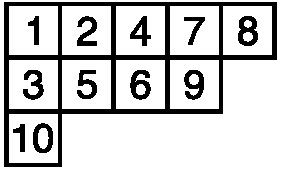
\includegraphics{Young_tableaux_for_541_partition.pdf}
	
	\begin{def*}[involution numbers]
		The number of distinct standard Young tableaux on $n$ entries is given by the \textbf{involution numbers}
		\[1, 1, 2, 4, 10, 26, 76, 232, 764, 2620, 9496, \dots.\]
	\end{def*}
	\begin{def*}[semistandard tableau]
		A tableau is called \textbf{semistandard}, or column strict, if the entries weakly increase along each row and strictly increase down each column.
	\end{def*}
	
	\begin{ytableau}
		 1  & 2 &  2&4&7\\
		 3 & 5 & 6&9&\none \\
		 8&\none&\none&\none&\none\\
	\end{ytableau}
		
	\begin{def*}[weight of tableau]
		Recording the number of times each number appears in a tableau gives a sequence known as the \textbf{weight of the tableau}.
	\end{def*}
	\begin{rem*}
		The standard Young tableaux are precisely the semistandard tableaux of weight $(1,1,\dots,1)$, which
		requires every integer up to $n$ to occur exactly once.
	\end{rem*}

	\subsubsection{G-module continued}\label{subsubsecGModule2}
	Given a group $G$ and a field $K$, there exists a unital associative algebra $(K[G],+,\cdot,*)$
	of $K$-valued functions on $G$ with finite support.
	
	For any $\lambda\in K[G]$, one can construct an endomorphism on the group algebra $K[G]$
	\[ \alpha \mapsto \alpha* \lambda,\forall \alpha\in K[G]. \]
	
	The image of such endomorphism is a linear subspace $(V_\lambda,+,\cdot)$ of $K[G]$ over $K$:
	\[V_\lambda=\set{\alpha*\lambda\in K[G]|\alpha \in K[G] }. \]
	
	The regular representation $\rho\colon G\to K[G]$ of the group:
	\[\rho(g)=e_g,\]
	acts on $V_\lambda$ same as the algebra multiplication:
	\[\rho(g)(\alpha*\lambda)=e_g*\alpha*\lambda,\forall \alpha*\lambda\in V_\lambda. \]
	
	For any  $\alpha*\lambda\in V_\lambda$, and $\beta\in K[G]$,
	\[\beta * (\alpha*\lambda) = (\beta*\alpha)*\lambda \in V_\lambda. \]
	Therefore $\rho(g)(V_\lambda)=V_\lambda$, \ie, $\rho(g)\in\End(V_\lambda)$.
	
	For any $\alpha*\lambda\in V_\lambda$ and $g\in G$,
	there exist $\gamma=e_{g^{-1}}*\alpha*\lambda\in V_\lambda$
	such that
	\[\rho(g)(\gamma)=\alpha*\lambda, \]
	so $\rho(g)\in \GL(V_\lambda)$ is an isomorphism.
	And thus it is a representation on $V_\lambda$.
	\subsubsection{Main Text}

	
	\red{Young diagrams can be used to describe projection operators for the 
		regular representation, which will then give the irreducible representations of
		$\mathfrak{S}_d$.}
	
	If $\inte_d=\bigcup_i \lambda_i$ and $\lambda_i$ also represents the index set represented by
	the $i$-th row of the Young tableau,
	then
	\[g\in P_\lambda\iff \forall \lambda_i [g(\lambda_i)=\lambda_i].\]
	
	For example, given the following tableau,
	
	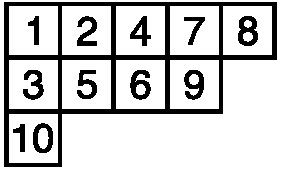
\includegraphics{Young_tableaux_for_541_partition.pdf}
	
	we have
	\[\lambda_1=\set{1,2,4,7,8},\lambda_2=\set{3,5,6,9},\lambda_3=\set{10}.\]
	
	Then $(12478)(396)\in P_\lambda$ but $(13)\notin P_\lambda$.
	
	\[\card{P}=\prod_{i}\card{\lambda_i}!.\]
		
	\begin{eq}
		For a partition $\lambda$, define two elements in $\co[\mathfrak{S}_d]$:
		\[a_\lambda=\sum_{g\in P}e_g,b_\lambda=\sum_{g\in Q}\sgn (g)e_g.\]
	\end{eq}
	
	$a_\lambda$ averages out everything within each row in the permutation representation $\co^d$
	with basis $(e_1,e_2,\dots,e_d)$:
	\[ \sum_{k=1}^dx_ke_k\mapsto \card{P}\sum_i\left(\frac{1}{\card{\lambda_i}}\sum_{j\in\lambda_i} x_j\right)\sum_{k\in\lambda_i}e_k.  \]
	
	$a_\lambda$ acting on $V^{\otimes d}=\bigotimes_i V^{\otimes \lambda_i}$
	as permutation within each $V^{\otimes \lambda_i}$ and then average them out,
	making it a symmetric tensor product space:
	
	\begin{centikzcd}\label{figAlambdaOnVd}
		V^{\otimes d} \ar[r,"a_\lambda"]&\bigotimes_i\Sym^{\lambda_i} V\\
	\end{centikzcd}



	Similarly, $\sgn$ gives the exterior product.
	
	\begin{eq}
		\[c_\lambda=a_\lambda b_\lambda.\]
	\end{eq}
	
	\begin{tthm}
		Irreducible representation of $\mathfrak{S}_d$ $\sim$ partition of $d$ $\sim$ conjugacy class of $\mathfrak{S}_d$.
	\end{tthm}

	\begin{prop}
		The following Young diagram corresponds to the alternating representation of $\mathfrak{S}_d$.
		
		\begin{ytableau}
			1\\
			2\\
			\none[\vdots]\\
			d\\
		\end{ytableau}
	\end{prop}
	\begin{proof}
		Let $G=\mathfrak{S}_d$.
		Then
		\begin{eqlong}
			P&=\set{e},\\
			Q&=G,\\
			a&=1,\\
			b&=\sum_{g\in G}\sgn(g)e_g,\\
			c&=\sum_{g\in G}\sgn(g)e_g,\\
			\co[G]\cdot c&=\sum_{h\in G}\sum_{g\in G}w_h\sgn(g)e_{hg}\\
			&=
			\sum_{h\in G}w_h\sgn(h^{-1})\sum_{g'\in G}\sgn(g')e_{g'}\\
			&=\co\cdot\sum_{g'\in G}\sgn(g')e_{g'},\\
		\end{eqlong}
		where $g'=hg$.
		
		For a permutation $p\in\mathfrak{S}_d$ and $x\in \co$,
		\[\begin{aligned}
			e_p\cdot x\cdot\sum_{g'\in G}\sgn(g')e_{g'}&=\sgn(p^{-1})\cdot x\cdot\sum_{g''\in G}\sgn(g'')e_{g''}\\
			&=\sgn(p)\cdot x\cdot\sum_{g''\in G}\sgn(g'')e_{g''}\\
			&=\begin{cases}
				x\cdot\sum_{g''\in G}\sgn(g'')e_{g''}&p\in \mathfrak{A}_d\\
				-x\cdot\sum_{g''\in G}\sgn(g'')e_{g''}&p\notin \mathfrak{A}_d\\
			\end{cases}
			,\\
		\end{aligned} \]
		where $g''=pg'$. This is the alternating representation.
	\end{proof}

	\begin{lem}
		\begin{eqlong}
			P_\lambda=Q_{\lambda'},\\
			Q_\lambda=P_{\lambda'}.\\
		\end{eqlong}
	\end{lem}
	\begin{def*}[tensor product of representations]
		If $V_{1},V_{2}$ are linear representations of a group $G$,
		then their tensor product is the tensor product of vector spaces $V_{1}\otimes V_{2}$
		with the linear action of $G$ uniquely determined by the condition that
		\[g\cdot (v_{1}\otimes v_{2})=(g\cdot v_{1})\otimes (g\cdot v_{2}).\]
	\end{def*}
	\begin{exe*}
		(a) \red{TODO}
		
		(b) $(Aa_\lambda)b_\lambda=A(a_\lambda b_\lambda)$.
		
		$(Ab_\lambda)a_\lambda=A(b_\lambda a_\lambda)$.
		
		And from(a): $A(b_\lambda a_\lambda)\cong A(a_\lambda b_\lambda)$.
		
		(c) \red{TODO, maybe using $c_\lambda^2=nc_\lambda$?}
		Let $G=\mathfrak{S}_d$. Then
		
		\begin{eqlong}
			V_\lambda&=Aa_\lambda b_\lambda=A\sum_{a\in P_\lambda}e_a\sum_{b\in Q_\lambda}\sgn(b)e_b,\\
			U'&=\co\cdot\sum_{g\in G}\sgn(g)e_g,\\
			\therefore V_\lambda \otimes U'&=A\sum_{a\in P_\lambda}\sum_{b\in Q_\lambda}\sum_{g\in G}
			\sgn(b)\sgn(g)e_ae_b\otimes e_g,\\
		\end{eqlong}
		
		Since $g\mapsto\sgn(g)$ and $g\mapsto e_g$ are group homomorphisms,
		and left action of $ab$ on $G$ permutes the group,
		and $\sgn(a)=\sgn(a^{-1})$,
		we have ($g'=abg$)
		\[V_\lambda \otimes U'=A\sum_{a\in P_\lambda}\sum_{b\in Q_\lambda}\sum_{g'\in G}
		\sgn(a)\sgn(g')e_ae_b\otimes e_{b^{-1}a^{-1}g'}. \]
	
		Consider the left action of $e_h$ on the tensor product space:
		\begin{eqlong}
			\alpha\sum_{a\in P_\lambda}\sum_{b\in Q_\lambda}\sum_{g'\in G}
			\sgn(a)\sgn(g')e_{hab}\otimes e_{h(ab)^{-1}g'}
		\end{eqlong}
	
		Note that $P_\lambda=Q_{\lambda'}$ and $Q_\lambda=P_{\lambda'}$,
		\begin{eqlong}
			V_{\lambda'}&=Aa_{\lambda'} b_{\lambda'}\cong Ab_{\lambda'} a_{\lambda'}=A\sum_{a\in Q_{\lambda'}}\sgn(a)e_a\sum_{b\in P_{\lambda'}}e_b=A\sum_{a\in P_{\lambda}}\sum_{b\in Q_{\lambda}}\sgn(a)e_{ab},\\
			%V_{\lambda'}&=A\sum_{b\in P_{\lambda'}}e_b\sum_{a\in Q_{\lambda'}}\sgn(a)e_a=A\sum_{b\in Q_{\lambda}}e_b\sum_{a\in P_{\lambda}}\sgn(a)e_a,\\
		\end{eqlong}
		
	\end{exe*}
	\begin{exe}
		All trivial and alternating representations are already derived.
		
		$\mathfrak{S}_2$
		
		See text.
				
		$\mathfrak{S}_3$
		
		For the standard representation:
		
		\begin{ytableau}
			1&2\\
			3\\
		\end{ytableau}
	
		\begin{eqlong}
			P&=\set{(1),(12)},\\
			Q&=\set{(1),(13)},\\
			a_\lambda&=1+e_{(12)},\\
			b_\lambda&=1-e_{(13)},\\
			c_\lambda=a_\lambda b_\lambda&=1+e_{(12)}-e_{(13)}-e_{(132)},\\
			e_{(12)}c_\lambda&=e_{(12)}+1-e_{(132)}-e_{(13)}=c_\lambda,\\
			e_{(123)}c_\lambda&=e_{(123)}+e_{(13)}-e_{(23)}-1,\\
			e_{(13)}c_\lambda&=e_{(123)}e_{(12)}c_\lambda=e_{(123)}c_\lambda,\\
			e_{(23)}c_\lambda&=e_{(23)}+e_{(132)}-e_{(123)}-e_{(12)}=-(1+e_{(13)})c_\lambda,\\
			e_{(132)}c_\lambda&=e_{(23)}e_{(12)}c_\lambda=-(1+e_{(13)})c_\lambda.\\
		\end{eqlong}
		Therefore, $c_\lambda$ and $e_{(13)}c_\lambda$ form the basis.
		
		\begin{eqlong}
			e_{(12)}
			\begin{pmatrix}
				1\\e_{(13)}
			\end{pmatrix}c_\lambda=
		\begin{pmatrix}
			e_{(12)}\\e_{(132)}
		\end{pmatrix}c_\lambda=
			\begin{pmatrix}
				1& 0\\
				-1&-1\\
			\end{pmatrix}
			\begin{pmatrix}
				1\\e_{(13)}
			\end{pmatrix}c_\lambda,\\
			e_{(123)}
			\begin{pmatrix}
				1\\e_{(13)}
			\end{pmatrix}c_\lambda=
		\begin{pmatrix}
		e_{(123)}\\e_{(23)}
	\end{pmatrix}c_\lambda=
			\begin{pmatrix}
				0& 1\\
				-1&-1\\
			\end{pmatrix}
			\begin{pmatrix}
				1\\e_{(13)}
			\end{pmatrix}c_\lambda.
		\end{eqlong}
		So $\Tr(e_{(12)})=0,\Tr(e_{(123)})=-1$.
		
		$\mathfrak{S}_4,\mathfrak{S}_5$: \red{TODO}
		
	\end{exe}	
	\begin{exe*}
		$\ext{s}V\sim$ a hook.
	\end{exe*}
	\begin{eq}
		\[
		\begin{aligned}
			P_j(x)&=\sum_{i=1}^{k}x_k^j,\\
			\Delta(x)&=\prod_{i<j}(x_i-x_j).\\
		\end{aligned}
		\]
	\end{eq}
	\begin{eq}
		\[f(x)=\sum_{l_1}\dots\sum_{l_k}[f(x)]_{(l_1,\dots,l_k)}\prod_{j=1}^{k}x_j^{l_j}
		.\]
	\end{eq}
	\begin{eq}
		\[l_j=\lambda_j+k-j.\]
	\end{eq}
	\begin{eq}
		\[\chi_\lambda(C_\mathbf{i})=\left[\Delta(x)\prod_{j=1}^dP_j(x)^{i_j}\right]_{(l_1,\dots,l_k)}.\]
	\end{eq}

	For the following Young diagram:
	
	\begin{ytableau}
		1&2\\
		3&4\\
		5\\
	\end{ytableau}
	
	\[d=5,\lambda=(2,2,1),k=3,l=(4,3,1).\]
	
	If we want to calculate the character of $(123)$, then $\mathbf{i}=(2,0,1,0,0)$.
	Hence we calculate the coefficient:
	\[[(x_1-x_2)(x_2-x_3)(x_1-x_3)(x_1+x_2+x_3)^2(x_1^3+x_2^3+x_3^3)]_{(4,3,1)}, \]	
	which gives
	\[\chi_{(2,2,1)}(C_{\mathbf{i}})=-1.\]
	
	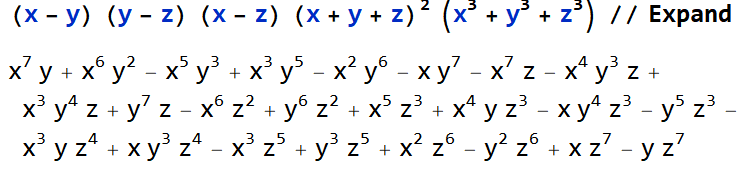
\includegraphics[scale=0.8]{frobenius_example}
	
	This corresponds to $W$.

	\red{Schur polynomials}
	
	\red{Vandermonde determinant}
	
	\begin{eq}
		\[\dim V_\lambda=\frac{d!}{\prod_{j=1}^kl_j!}\prod_{i<j\le k}(l_i-l_j).\]
	\end{eq}

	\begin{def*}[hook length]
		The \textbf{hook length} of a box in a Young diagram is the number of squares directly below 
		or directly to the right of the box, including the box once.
	\end{def*}
 
	In the following diagram, each box is labeled by its hook length:
	
	\begin{ytableau}
		6&4&3&1\\
		4&2&1\\
		1\\
	\end{ytableau}

	\begin{eq}
		\[\dim V_\lambda=\frac{d!}{\prod_{j=1}^d {L}_j},\]
		where $L$ is the hook length.
	\end{eq}

	\begin{exe*}
		\red{TODO}
	\end{exe*}
	\begin{exe*}
		\red{TODO}
	\end{exe*}
	\begin{exe*}
	\red{TODO}
	\end{exe*}
	\begin{exe*}
	\red{TODO}
	\end{exe*}
	\begin{exe}
		\red{TODO}
	\end{exe}
	\begin{eq}
		\red{TODO}
		
		\[\chi_\lambda((12\dots m)).\]
	\end{eq}
	\begin{def*}[rank, characteristics]
		
		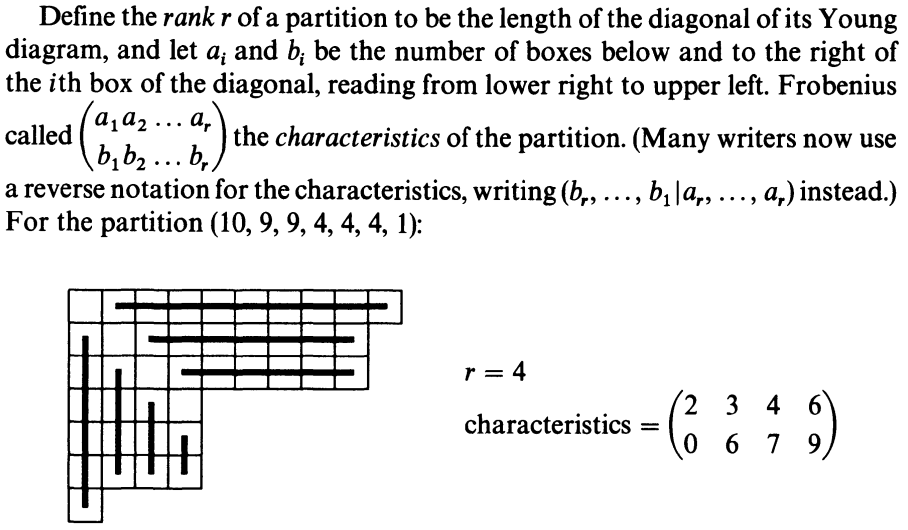
\includegraphics[scale=0.4]{rank_characteristics}
	\end{def*}

	\begin{exe*}
		\red{TODO}
	\end{exe*}

	\begin{exe*}
		\red{TODO}
	\end{exe*}

	\subsection{Irreducible representations of $\mathfrak{S}_d$}
	
	\red{TODO}
	\subsection{Proof of Frobenius's formula}
	
	\red{TODO}
	
	\section{Representations of $\mathfrak{A}_d$ and $\GL_2(\mathbb{F}_q)$}
	\subsection{Representations of $\mathfrak{A}_d$}
	
	\subsubsection{Basic Property of Subgroup of Index 2, Normal Subgroup}
	\begin{lem}\label{lemHalfGroupEvenOdd}
		If $H$ is a subgroup of $G$ with index 2, then 
		\begin{eqlong}
			h,h'\in H\implies&hh'\in H,\\
			s\in G\setminus H\iff &s^{-1}\in G\setminus H,\\
			r,s\in G\setminus H\implies& rs\in H,\\
			s\in G\setminus H\land h\in H\implies& sh\notin H\land hs \notin H.\\
		\end{eqlong}
	\end{lem}
	\begin{proof}
		The first relation is a result of closed multiplication in the group $H$.
		
		$G$ can be divided into two disjoint left cosets: $H$ and $G\setminus H$ (definition of index,
		\ref{lemCosetsCoverAll}, \ref{lemDisjointLeftCoset}).
		
		Since $s\in G\setminus H$ and $G\setminus H$ is a left coset,
		$\therefore sH=G\setminus H$ (\ref{lemSameCoset}).
		If $s^{-1}\in H$, then by definition of coset, $e=ss^{-1}\in sH=G\setminus H$,
		which contradicts with $e\in H$.
		Therefore $s^{-1}\notin H$.
		Since $(s^{-1})^{-1}=s$, the reverse is also true.
		
		If $r,s\in G\setminus H$, then $r^{-1}\in G\setminus H$.
		From \ref{lemgHg'H}, we know $rs=(r^{-1})^{-1}s\in H$.
		
		The last equation is a result of disjoint left/right cosets.
	\end{proof}
	\begin{prop}\label{lemHalfGroupNormal}
		A subgroup of index 2 is always normal.
	\end{prop}
	\begin{proof}
		Let $G$ be a group and $H$ be its subgroup of index 2.
		
		Since $H$ is a group, $\therefore h,h'\in H\implies hh'h^{-1}\in H$.
		
		If $s\in G\setminus H, h\in H$, then (\ref{lemHalfGroupEvenOdd})
		\[ s^{-1}\in G\setminus H, sh\in G\setminus H ,\]
		leading to (\ref{lemHalfGroupEvenOdd})
		\[ shs^{-1}\in H.\]
	\end{proof}
	\begin{rem*}
		Alternatively, $G\setminus H = sH=Hs\implies H$ commutes with any $s\notin H$.
		\url{https://crypto.stanford.edu/pbc/notes/group/normal.html}
	\end{rem*}
	\begin{prop}\label{lemNormalSubGroupConjugacy}
		If $N$ is a normal subgroup of $G$, then the conjugacy classes of $G$ must be either subset of $N$ or subset of $G\setminus N$.
	\end{prop}
	\begin{proof}
		If $n\in N$, then from definition of normal subgroup, $\forall g\in G[gng^{-1}\in N]$.
		
		If $s\in G\setminus N$ but $\exists g\in G[gsg^{-1}\in N]$.
		Let $n'=gsg^{-1}\in N$, then $s=hn'h^{-1}\in N$ where $h=g^{-1}\in G$, which is contradicting.
	\end{proof}
	\begin{cor}\label{lemHalfGroupConjugacy}
		Let $G$ be a group and $H$ be its subgroup of index 2.
		The conjugacy classes of $G$ must be either subset of $H$ or subset of $G\setminus H$.
	\end{cor}
	\begin{proof}
		\ref{lemNormalSubGroupConjugacy},
		\ref{lemHalfGroupNormal}.
	\end{proof}

	\begin{prop}
		Let $G$ be a group and $H$ be its subgroup of index 2.
		Then any conjugacy class $C$ of $G$ is either a conjugacy class of $H$
		or the union of two conjugacy classes of $H$ of equal size.
	\end{prop}
	\begin{proof}
		\red{TODO}
	\end{proof}
	\subsubsection{Main Text}

	\begin{def*}[nontrivial representation]
		Given a subgroup $H$ of group $G$ with index 2,
		the \textbf{nontrivial representation} of $G$ obtained 
		from the two representations of $G/H$, denoted $U'$, is
		\[\chi_{U'}(g)=\begin{cases}
			1&g\in H\\
			-1&g\notin H\\
		\end{cases}. \]
	\end{def*}
	\begin{rem*}
		This is a valid representation due to \ref{lemHalfGroupEvenOdd}.
		
		This is the \textbf{alternating representation} in $\mathfrak{S}_d$.
	\end{rem*}

	\begin{def*}[conjugate representation]
		If $W$ is any representation of $H$ as a subgroup of $G$ with index 2,
		there is a \textbf{conjugate representation} $W'$ defined as
		\[\chi_{W'}(h)=\chi_{W}(tht^{-1}), \]
		where $t\in G\setminus H$.
	\end{def*}
	\begin{prop}
		Conjugate representation is unique up to isomorphism.
	\end{prop}
	\begin{proof}
		\[tht^{-1}\in H \] because \ref{lemHalfGroupNormal}.
		
		\red{TODO: Prove conjugate representation \textit{is} a representation of $H$.}
		
		Given $\chi_{W'}(h)=\chi_{W}(tht^{-1})$, and $\chi_{W''}(h)=\chi_{W}(shs^{-1})$,
		where $t,s\in G\setminus H$.
		
		Then $t^{-1}s\in H$ (\ref{lemHalfGroupEvenOdd}), denoted as $n=t^{-1}s$, \ie, $s=tn$.
		
		Therefore
		\[\chi_{W''}(h)=\chi_{W}((tn)h(tn)^{-1})=\chi_{W}(t(nhn^{-1})t^{-1})=\chi_{W'}(nhn^{-1})=\chi_{W'}(h),\]
		because $nhn^{-1}$ and $h$ are in the same conjugacy class of $H$.
		%so it must be equal to $\chi_{W'}(h)$.
	\end{proof}
	\begin{prop}\label{lemSelfConjugateRestriction}
		A representation is self-conjugate if and only if it is a restriction.
	\end{prop}
	\begin{proof}
		If $W$ as a representation of $H$ (a subgroup of $G$ of index 2)
		is a restriction of $V$, a representation of $G$, then
		$W$ must be self-conjugate because for any $t\in G\setminus H,h\in H$,
		\[\chi_W(tht^{-1})=\chi_V(tht^{-1})=\chi_V(h)=\chi_W(h)\]
		as $tht^{-1}$ and $h$ are in the same conjugate class of $G$.

		If $W$ as a representation of $H$ is self-conjugate,
		then for any $g\in G,h\in H$ ($ghg^{-1}\in H $ because \ref{lemHalfGroupNormal}),
		\[f(ghg^{-1})=2\chi_W(ghg^{-1})=2\chi_W(h)=f(h),\]
		where $f$ is a class function of $G$
		\[ f(g)=\begin{cases}
			2\chi_W(g)&g\in H\\
			0& g\notin H\\
		\end{cases}, \]
		which is possible because \ref{lemHalfGroupConjugacy}.
		
		\red{Prove this: $f$ is the character of $\Ind W$ and it is direct sum of two representations whose restriction
		is $W$.}
	\end{proof}

	\begin{prop}\label{lemIndResU=U+U'}
		If $U$ is a representation of group $G$
		and $W$ a representation of subgroup $H$ of index 2, 
		then \[\Ind(\Res(U))=U\oplus U'.\]
	\end{prop}
	\begin{proof}
		From Exercise 3.16(a), we know that 
		\[\Ind(\Res(U)) = U \otimes P,\]
		where $P$ is the permutation representation of $G$ on $G/H$.
		
		For $h\in H$, since $hH=H$ (\ref{lemSameCoset}) and $h(G\setminus H)=G\setminus H$ (\ref{lemHalfGroupEvenOdd}),
		$\chi_P(h)=2$.
		
		For $t\in G\setminus H$, since $tH=G\setminus H, t(G\setminus H)=H$ (\ref{lemHalfGroupEvenOdd}),
		$\chi_P(t)=0$.
		
		Therefore $P=T\oplus T'$, where $T$ is the trivial representation and $T'$ is the alternating representation.
		Hence, $\Ind(\Res(U))=U\oplus U'$ where $U'=U\otimes T'$.
	\end{proof}

	\begin{pprop}
		Let $V$ be an irreducible representation of $G$, and let $W$
		be the restriction of $V$ to $H$. Then exactly one of the following holds:
		$\dots$
	\end{pprop}
	\begin{proof}
		Since $V$ is irreducible representation of $G$
		we have $(\chi_V,\chi_V)_G=1$.
		As $H$ has index 2,
		\[2\card{H}=\card{G}=\sum_{h\in H}\abs{\chi_V(h)}^2+\sum_{t\notin H}\abs{\chi_V(t)}^2 \]
		
		But
		\[\sum_{h\in H}\abs{\chi_V(h)}^2=\sum_{h\in H}\abs{\chi_W(h)}^2=\card{H}(\chi_W,\chi_W)_H\]
		is multiple of $\card{H}$.

		The multiple must be 1 or 2, because both terms are non-negative and their sum is $2\card{H}$.
		
		\begin{itemize}
			\item If $\sum_{h\in H}\abs{\chi_V(h)}^2=\card{H}$, then $W$ is a irreducible representation 
			because $(\chi_W,\chi_W)_H=1$. In this case 
			\[\sum_{t\notin H}\abs{\chi_V(t)}^2=\card{H}>0\implies 
			\exists t\notin H[\chi_V(t)\ne 0]\]
			which means $V$ is not isomorphic to $V'=V\otimes U'$ where $U'$ is the alternating representation.
			
			$W$ is self-conjugate because \ref{lemSelfConjugateRestriction}.
			$\Ind W=\Ind \Res V=V\oplus V'$ because \ref{lemIndResU=U+U'}.
			
			\item If $\sum_{h\in H}\abs{\chi_V(h)}^2=\card{G}$, then $W$ is a direct sum of two irreducible representations 
			because $(\chi_W,\chi_W)_H=2$. Then $W$ is a direct sum of two different irreducible representations
			(Exercise 2.33(b)).
			In this case 
			\[\sum_{t\notin H}\abs{\chi_V(t)}^2=0\implies 
			\forall  t\notin H[\chi_V(t)=0]\]
			which means $V$ is isomorphic to $V'=V\otimes U'$ where $U'$ is the alternating representation.
			
			Let $W=W'\oplus W''$, \red{prove $W'$ is conjugate to $W''$.}
			
			\red{Prove $\Res(\Ind W)$ is the direct sum of $W$ and its conjugate (Exercise 3.l9)}
			
			\red{Prove $V\cong \Ind W' \cong \Ind W''$.}
			
			\red{Prove Each irreducible representation of H arises uniquely in this way}
		\end{itemize}
	\end{proof}

	
	\begin{exe*}
		\red{TODO}
	\end{exe*}
	\red{TODO till end of subchapter}
	
	\begin{pprop}
		\red{TODO}
	\end{pprop}
	\begin{exe*}
		\red{TODO}
	\end{exe*}

	\begin{exe*}
		\red{TODO}
	\end{exe*}

	\subsection{Representations of $\GL_2(\mathbb{F}_q)$ and $\SL_2(\mathbb{F}_q)$}
	\subsubsection{Finite Field}
	\begin{def*}[prime power]
		A \textbf{prime power} is a positive integer power of a single prime number. 
	\end{def*}
	\begin{def*}[Galois field]
		A \textbf{finite field} or \textbf{Galois field} is a field that contains a finite number of elements. 
	\end{def*}
	\begin{thm}
		A finite field of order $q$ exists if and only if $q$ is a prime power $p^k$ (where $p$ is a prime number and $k$ is a positive integer).
	\end{thm}
	\begin{thm}
		All fields of the same order are isomorphic.
		Moreover, a field cannot contain two different finite subfields with the same order.
	\end{thm}
	\begin{rem*}
		One may therefore identify all finite fields with the same order, and they are unambiguously denoted $\mathbb  {F}_{q}$, $F_q$ or $\operatorname{GF}(q)$.
	\end{rem*}
	\begin{thm}
		The characteristic of the field $\mathbb{F}_{p^k}$ ($p$ as a prime number and $k$ a positive integer) is $p$.
	\end{thm}

	\begin{rem*}
		Finite field of characteristic $p$ is $\field_{p^k}$ where $k$ is a positive integer.
		%The elements can be expressed as $k$-tuple of $0$'s and $1$'s.
		%Assume the index of the $k$-tuple is $0$-based.
		%Addition is pairwise, defined as
		%\[ (x+y)_i=x_i+y_i.\]
		%The multiplication is
		%\[ (xy)_i=\sum_{j=0}^{k-1} x_jy_{(i-j)\bmod k}. \]
		%The additive identity is the $k$-tuple with all $0$s,
		%and the multiplicative identity if the $k$-tuple with only $1$ at $0$-th index and $0$ otherwise.
		%
		%Alternatively, it is
		It can be constructed as
		the quotient polynomial ring
		\[\sum_{i=0}^{k-1} a_ix^i \in \field_p[x]/(P), \]
		where $a_i\in\field_p$ and $(P)$ is the two-sided ideal
		generated from an irreducible polynomial of degree $k$ in $\field_p[x]$.
		
		For example,
		\[ \begin{aligned}
			\field_4&=\field_2[x]/(x^2+x+1),\\
			\field_{p^2}&=\field_p[x]/(x^2+1),\\
		\end{aligned} \]
		where $p$ is an odd prime here.
	\end{rem*}

	\begin{prop}
		If $q$ is odd, $\field_q^*$ contains half of elements with square roots, and exactly 2 square roots.
		If $q$ is even, every element in $\field_q$ has a unique square root.
	\end{prop}
	\begin{proof}
		$x^2=y^2\implies x=y\lor x=-y$.
		
		For odd $q$, $x\ne-x\iff x\ne0$.
		So $x\sim-x$ forms a equivalence relation and thus equivalence classes in $\field_q^*$.
		Every equivalence class has a distinct (unique) square, therefore exactly half of the multiplicative group
		must have exactly 2 square roots.
		
		For even $q$, $x=-x$ (because $q$ must be a power of $2$, so the field must have characteristic of 2).
		So $x\sim-x$ forms a equivalence relation and thus equivalence classes (as a singleton) in $\field_q$.
		Every equivalence class has a distinct (unique) square, therefore all elements in the field
		must have exactly 1 square root.
	\end{proof}
	\begin{rem*}
		Also see \href{http://cap-lore.com/MathPhys/Field/finite/sqrt.html}{this proof}.
	\end{rem*}

	\begin{thm}\label{thmGF*Cyclic}
		The multiplicative group of a finite field is a cyclic group.
	\end{thm}
	\begin{def*}[primitive element]
		A \textbf{primitive element} of a finite field $\field_q$ is a generator of the multiplicative group of the field,
	\end{def*}
	\begin{thm}
		Primitive element must exist.
		Given $\alpha \in \field_q$, below statements are equivalent.
		\begin{itemize}
			\item $\alpha$ is a primitive element.
			\item $\alpha$ is a primitive $(q - 1)$th root of unity.
			\item Each non-zero element of $\field_q$ can be written as $\alpha^i$ for some integer $i$.
		\end{itemize}
	\end{thm}
	
	\begin{def*}[Euler's totient function]
		The \textbf{Euler's totient function} $\phi\colon\inte^+\to\inte^+$
		is defined as $\phi(m)$
		counting the positive integers less than or equal to $m$
		which are relatively prime to $m$.
	\end{def*}
	\begin{thm}
		A finite cyclic group of order $m$ contains $\phi(m)$ generators.
	\end{thm}
	\begin{cor}
		The number of primitive elements in a finite field $\field_q$ is $\phi(q - 1)$,
		where $\phi$ is Euler's totient function.
	\end{cor}
%	
	\begin{prop}\label{propPrimNoSqrt}
		A primitive element of an odd-order finite field does not have square root.
	\end{prop}
	\begin{proof}
		Let $\varepsilon$ be the primitive element and assume $\alpha$
		as its square root.
		
		Then $\alpha^{q-1}=\varepsilon^{(q-1)/2}=1$ (property of cyclic group and $q$ is odd)
		which contradicts with the definition of primitive element (primitive $(q-1)$th root of unity).
	\end{proof}

	\begin{prop}\label{propPrimHasSqrtInExtension}
		A primitive element of an odd-order finite field $\field_q$ has two square roots in $\field_{q^{2n}}$
		where $n$ is a positive number.
	\end{prop}
	\begin{proof}
		Let $\varepsilon$ be the primitive element in $\field_q$
		and $\kappa$ be the primitive element in $\field_{q^{2n}}$.
		
		Therefore, \[\kappa^{q^{2n}-1}=(\kappa^{m})^{q-1}=1=\varepsilon^{q-1},\]
		where \[m=\sum_{i=0}^{2n-1}q^i\]
		is an even number (since $q$ is odd and number of terms is even).
		
		Since both are primitive root of unity,
		\[ \varepsilon=\kappa^m.\]
		Because $m$ is even, $\varepsilon$ must have square root(s).
	\end{proof}

	\subsubsection{Linear Groups}
	\begin{def*}[special linear group]
		The \textbf{special linear group} $\SL(n, F)$ or $\SL_n(F)$ of degree $n$ over a field $F$
		is the set of $n\times n$ matrices with determinant 1,
		with the group operations of ordinary matrix multiplication and matrix inversion.
	\end{def*}
	\begin{thm}
		The special linear group is the normal subgroup of the general linear group given by the kernel of the determinant
		\[\det\colon\GL(n,F)\to F\setminus\set{0}. \]
	\end{thm}

	\begin{thm}
		The center of a group is always a normal subgroup.
	\end{thm}

	\begin{def*}[projective space]
		Given a vector space $V$ over a field $K$, the \textbf{projective space} $\operatorname{P}(V)$
		is the set of equivalence classes of $V^*=V \setminus\set{\mathbf{0}}$ under the equivalence relation
		$\sim$ defined by $x \sim y$ if there is a nonzero element $\lambda$ of $K^*=K\setminus\set{0}$ such that $x = \lambda y$.
		Explicitly:
		\[\operatorname{P}(V)=\set{\set{\lambda x\in V^*|\lambda\in K^*}\in\power(V^*)|x\in V^*} .\]
	\end{def*}
	\begin{rem*}
		It can be viewed as a sphere in the $V^*$ space?
		Every element of the projective space is corresponding to a projective line in $V^*$.
	\end{rem*}

	\begin{def*}[projective linear group]
		The \textbf{projective (general) linear group} is the quotient group
		\[\PGL(V) = \GL(V)/\ZZ(V),\]
		where $\GL(V)$ is the general linear group of vector space $V$
		and $\ZZ(V)$ is the normal subgroup of all nonzero scalar transformations of $V$
	\end{def*}
	\begin{rem*}
		$\PGL$ is the induced action of the general linear group of a vector space $V$ on the associated projective space $\operatorname{P}(V)$. $\ZZ(V)$ are quotiented out because they act trivially on the projective space and they form the kernel of the action.
	\end{rem*}



	\begin{thm}
		$\ZZ(V)$ is the center of $\GL(V)$.
	\end{thm}


	\begin{def*}[projective special linear group]
		The \textbf{projective special linear group} is defined as
		\[\PSL(V) = \SL(V)/\SZ(V),\]
		where $\SL(V)$ is the special linear group over a vector space $V$
		and $\SZ(V)$ is the subgroup of scalar transformations with unit determinant.
	\end{def*}
	\begin{rem*}
		$\PSL$ is the induced action of the special linear group on the associated projective space.
	\end{rem*}

	\begin{thm}
		$\SZ(V)$ is the center of $\SL(V)$.
	\end{thm}
	\begin{thm}
		$\SZ(V)$ is the group of $n$th roots of unity in $F$,
		where $n$ is the dimension of $V$ over field $F$.
	\end{thm}

	General linear group can be considered as moving the axes and rulers on the axes.
	
	

	\subsubsection{Main Text}
	
	\paragraph{Introduction}
	\begin{def*}[GL2Fq]
		$\GL_2(\mathbb{F}_q)$ is the group of invertible $2 \times 2$ matrices with entries in the finite field 
		$\mathbb{F}_q$ with $q$ elements, where $q$ is a prime power.
	\end{def*}

	\begin{def*}[simple group]
		A \textbf{simple group} is a nontrivial group whose only normal subgroups are the trivial group and the group itself.
	\end{def*}

	Similar to irreducible representation?
	
	\paragraph{Borel Subgroup}
	
	\subparagraph{Cardinality}
	The Borel subgroup $B$ of $G=\GL_2(\field_q)$ has cardinality:
	\[\card{B}=q(q-1)^2, \]
	because in the form
	\[\begin{pmatrix}
		a&b\\
		0&d\\
	\end{pmatrix}, \]
	$a\ne0,d\ne0$ (otherwise not invertible).

	\subparagraph{Non-normal Subgroup}
	Given any $g\in G$, $x\in B$,
	\[(gxg^{-1})_{21} =\sum_i\sum_j g_{2i}x_{ij}(g^{-1})_{j1}=g_{21}x_{11}(g^{-1})_{11}+\sum_i g_{2i}x_{i2}(g^{-1})_{21} \]
	since $x_{21}=0$
	but this is not necessarily $0$. Therefore Borel subgroup is \textbf{not a normal subgroup} of $G$.
	
	If $x_{11}=x_{22}=1$, then
	\[(gxg^{-1})_{21}=g_{21}(g^{-1})_{11}+g_{22}(g^{-1})_{21}+g_{21}x_{12}(g^{-1})_{22}=g_{21}x_{12}(g^{-1})_{22}=\frac{x_{12}g_{21}g_{11}}{\det g}. \]
	Therefore
	\[N=\set{\begin{pmatrix}
			1&b\\0&1\\
	\end{pmatrix}} \]
	is \textbf{a subgroup but not normal subgroup} of $\SL_2(\field_q)$.
	
	For example, if
	$x=\begin{pmatrix}
		1&1\\0&1
	\end{pmatrix}\in N,g=\begin{pmatrix}
	1&0\\
	1&1\\
	\end{pmatrix}\in \SL_2(\field_q)$,
	then $g^{-1}=\begin{pmatrix}
		1&0\\-1&1\\
	\end{pmatrix}\in\SL_2(\field_q)$,
	and $gxg^{-1}=\begin{pmatrix}
		0&1\\-1&2
	\end{pmatrix}\notin B$ (it becomes $\begin{pmatrix}
	0&1\\1&0
	\end{pmatrix}$ if $q$ is power of 2).

	\subparagraph{Conjugacy classes of Borel subgroup}
	Given $x=\begin{pmatrix}
		a&b\\0&d
	\end{pmatrix}\in B$ and $s=\begin{pmatrix}
		a'&b'\\0&d'
	\end{pmatrix}\in B$, we have (since $d'\ne0$)
	\[sxs^{-1}=\begin{pmatrix}
		a&\frac{b'(d-a)+a'b}{d'}\\0&d
	\end{pmatrix}. \]

	Therefore there are three types of conjugacy classes.
	For any $b''\in\field_q$, if we want $sxs^{-1}=\begin{pmatrix}a&b''\\0&d\end{pmatrix}$,
	then
	\begin{enumerate}
		\item if $a\ne d$, then $a'=a-d,b'=b+b'',d'=d-a$.
		\item if $a=d,b\ne0,b''\ne0$, then $a'=b'',b'=0,d'=b$.
		\item if $a=d,b=b''=0$, then $a'=d'=1,b'=0$.
		%\item If $b\ne 0$,$b''\ne0$, then $a'=b'',b'=0,d'=b$.
		%\item If $b=0$ and $a\ne d$, then $a'=1,b'=b'',d'=d-a$.
	\end{enumerate}

	\begin{table}\label{tblConjBorel}
		\caption{Conjugacy classes of the Borel subgroup}
		\begin{centabular}{L|C|C}
			\text{Representative}&\text{Num Elements in Class}&\text{Num Classes}\\
			\hline
			a_x'=\begin{pmatrix}x&0\\0&x\end{pmatrix},x\ne0 &1&q-1\\
			b_x'=\begin{pmatrix}x&b\\0&x\end{pmatrix},x\ne0,b\ne0 &q-1&q-1\\
			c_{x,y}'=\begin{pmatrix}x&b\\0&y\end{pmatrix},xy\ne0,x\ne y &q&(q-1)(q-2)\\
		\end{centabular}
	\end{table}

	Therefore the number of conjugacy classes is $q(q-1)$ and total number of elements is $q(q-1)^2$.
	
	The conjugacy classes of $B$ is summarized in \ref{tblConjBorel}.

	\paragraph{Projective Line}

	Based on the definition of projective space,
	the \textbf{finite projective line} $L_{(1:0)}$, as an element of the projective space,
	is a subset of the 
	2-dimensional vector space $\field_q^2$
	such that
	\[L_{(1:0)}=\set{(a,0)\in \field_q^2|a\ne 0} .\]


	\paragraph{Transitive Group Action}
	\begin{def*}[transitive group action]
		The \textbf{action} of group $G$ on set $X$ is called		
		\textbf{transitive} if $X$ is non-empty and
		if for each pair $x, y$ in $X$ there exists a $g$ in $G$ such that $gx = y$, \ie,
		\[X\ne\emptyset \land \forall x\in X\forall y \in X\exists g\in G[gx=y]. \]
	\end{def*}


% For example, the action of the symmetric group of X is transitive, the action of the general linear group or the special linear group of a vector space V on V ∖ {0} is transitive, but the action of the orthogonal group of a Euclidean space E is not transitive on E ∖ {0} (it is transitive on the unit sphere of E, though).

	Based on the definition of projective space,
	Any element $x\in\mathbb{P}^1(\field_q)$ can be expressed as
	\[x = \set{ a(x_1,x_2)|a\in\field_q^*}, \]
	where $\field_q^*=\field_q\setminus\set{0}$ and $x_1x_2\ne0$.

	$G=\GL_2(\field_q)$ acts transitively on $\mathbb{P}^1(\field_q)$.
	This is because $G$ are isomorphisms (and therefore maps projective line onto projective line)
	and $G$ contains all isomorphisms (and therefore for any $x,y\in\mathbb{P}^1(\field_q)$ there exists
	a mapping $g\in G$ from $x$ onto $y$).
	
	\paragraph{Isotropy Group}
	\begin{def*}[isotropy group]
		An \textbf{isotropy group} is the group of isomorphisms from any object to itself in a groupoid.
		An isotropy representation is a representation of an isotropy group.
	\end{def*}

	For any $x=(r,0),y=(s,0)\in L_{(1:0)}$,
	$gx=y\implies g\in B$, because $0=y_2=g_{21}x_1+g_{22}x_2=g_{21}x_1$
	but $x_1=r\ne0$. Therefore $B$ contains the isotropy group on $L_{(1:0)}$.
	
	Given any $g=\begin{pmatrix}
		a&b\\0&d
	\end{pmatrix}\in B$ and $x=(r,0)\in L_{(1:0)}$,
	we have $gx=(ar,0)\in L_{(1:0)}$ because $a\ne0,r\ne0$.
	
	Also, $B$ acts transitively on $L_{(1:0)}$. For any $x=(r,0),y=(s,0)\in L_{(1:0)}$,
	we have $g\in B$
	such that
	$gx=y$,
	given 
	\[g = \begin{pmatrix}
		s/r&0\\
		0&1\\
	\end{pmatrix}, \]
	because $r\ne0,s\ne0$.
		
	Therefore, $BL_{(1:0)}=L_{(1:0)}$, concluding that $B$ is the isotropy group acting on $L_{(1:0)}$.
	
	\paragraph{The Order of $G$}
	
	The order of $G$ is the product of the cardinality of $\mathbb{P}^1(\field_q)$
	multiplied by the order of the isotropy group on one element in $\mathbb{P}^1(\field_q)$.
	
	Since $\field_q^*$ is a multiplicative group,
	\[\therefore a(1,x)=(1,y)\iff a=1\implies x=y,\]
	where $a,x,y\in\field_q$.
	
	Therefore, $(1,x)\in \field_q^2$ are $q$ representatives of $q$ different projective lines
	in the space $\mathbb{P}^1(\field_q)$.
	
	Since $\field_q^*$ is a multiplicative group (meaning, multiplicative inverse exists),
	any vector in $\field_q^2$ with nonzero first coordinate
	is a scalar product of a nonzero scalar with one of the vectors of form $(1,x)$.
	
	Easy to prove that $(0,1)$ is the last remaining equivalent class in $\mathbb{P}^1(\field_q)$, so
	\[\card{\mathbb{P} ^1(\field_q)}=q+1, \]
	and therefore
	\[ \card{G} = \card{B}\card{\mathbb{P} ^1(\field_q)}=(q-1)^2q(q+1). \]
	
	\paragraph{Field Extension}
	\begin{def*}[field extension]
		If $K$ is a subfield of $L$,
		then $L$ is an \textbf{extension field} or simply extension of $K$,
		and this pair of fields is a \textbf{field extension}.
		Such a field extension is denoted $L / K$ (read as ``$L$ over $K$'').
	\end{def*}
	\begin{def*}[intermediate field]
		If $L$ is an extension of $F$, which is in turn an extension of $K$,
		then $F$ is said to be an \textbf{intermediate field} (or intermediate extension or subextension) of $L / K$.
	\end{def*}
	
	\begin{thm}
		Given a field extension $L / K$,
		the larger field $L$ is a $K$-vector space.
		The dimension of this vector space is called the degree of the extension and is denoted by $[L : K]$.
	\end{thm}
	\paragraph{The Cyclic Subgroup}
	\begin{thm}
		Any finite group has some cyclic subgroup.
	\end{thm}

	\begin{prop}
		Let $\varepsilon$ be a primitive element of an odd-order finite field $\field_q$.
		Then one of the square roots of $\varepsilon$ together with $1$ forms the basis of $\field_{q^2}=\field_q(1,\sqrt{\varepsilon})$.
	\end{prop}
	\begin{proof}
		Clearly $\field_q$ is a subfield of $\field_{q^2}$ (\red{need proof})
		and therefore $\field_{q^2}/\field_q$ is a field extension,
		and the $\field_{q^2}$ can be viewed as a 2-dimensional vector space over $\field_q$.
		
		Since $\field_q^*$ is a cyclic group, it must have a multiplicative generator (primitive element), denoted $\varepsilon$.
		Since it is a generator, it must not have square root in $\field_q$ if $q$ is odd (\ref{propPrimNoSqrt}).
		
		Denote one of its square root in $\field_{q^2}$ as $\sqrt{\varepsilon}$ (existence: \ref{propPrimHasSqrtInExtension})
		and therefore this combined with $1$
		form a basis of the vector space $\field_{q^2}$.
	\end{proof}
	\begin{rem*}
		Note, it is possible that $-1$ has (two) square root(s) in a odd-order finite field (\eg, $\field_9$, 
		see \href{https://www.chegg.com/homework-help/questions-and-answers/11-let-f9-finite-field-9-elements-addition-multiplication-tables-f9-given-next-page-descri-q13298041}{this}, $b^2=e^2=2=-1$).
	\end{rem*}

	\begin{prop}
		Given odd $q$ and $x,y\in \field_q$ but $x\ne0\lor y\ne0$,
		\[x+y\sqrt{\varepsilon} \mapsto \begin{pmatrix}
			x&\varepsilon y\\y&x\\
		\end{pmatrix}\] is a group isomorphism from $\field_{q^2}^*$ onto $K\subseteq\GL_2(\field_q)$.
	\end{prop}
	\begin{proof}
		First prove $\bfA=\begin{pmatrix}
			x&\varepsilon y\\y&x\\
		\end{pmatrix}\in\GL_2(\field_q)$.
	
		Note that
		\[\det\bfA=x^2-\varepsilon y^2\]
		which becomes nonzero if either $x$ or $y$ is zero (the other must be nonzero, and $\varepsilon\ne0$).

		Since $\varepsilon$ is a primitive $(q-1)$th root of unity, where $q-1$ is even,
		$\therefore$ odd power of $\varepsilon$ is not $1$.
		
		If $x\ne0,y\ne0$, then
		\[\det\bfA=x^2-\varepsilon y^2=\varepsilon^{2r}-\varepsilon^{2s+1}=
		\varepsilon^{2r}(1-\varepsilon^{2s-2r+1})\ne0, \]
		%because $\varepsilon$ is a generator
		because $2s-2r+1$ is odd ($\implies 1-\varepsilon^{2s-2r+1}\ne0$)
		and $\varepsilon\ne0$ ($\implies\varepsilon^{2r}\ne0$),
		$x\ne0,y\ne0$ ($\implies x,y$ can be expressed as power of the multiplicative generator $\varepsilon$).
		Therefore $\bfA\in\GL_2(\field_q)$.
		
		Since $(1,\sqrt{\varepsilon})$ forms a basis of $\field_{q^2}$,
		the coefficients $x,y$ are unique,
		$\therefore$ this map is injective.
		Therefore it is a bijection onto its image.
		
		Below shows this is a group homomorphism.
		\[\begin{aligned}
			&(x+y\sqrt{\varepsilon} )(u+v\sqrt{\varepsilon} )=
			(xu+yv\varepsilon) + (xv+yu)\sqrt{\varepsilon}\\
			\mapsto&
			\begin{pmatrix}
				xu+yv\varepsilon&\varepsilon(xv+yu)\\
				xv+yu&xu+yv\varepsilon
			\end{pmatrix}
			= \begin{pmatrix}
				x&\varepsilon y\\
				y&x
			\end{pmatrix}\begin{pmatrix}
			u&\varepsilon v\\
			v&u
		\end{pmatrix}\\
		\end{aligned} 
		 \]
	\end{proof}

	\paragraph{Conjugacy classes in $G$}
	\begin{rem*}
		Conjugacy classes in $G$:
		\begin{enumerate}
			\item 
			$a_x\in\ZZ(G)$ so their conjugacy classes are singletons (note $x\ne0$).
			
			\item
			Given $a\ne0$,
			\[
			\begin{aligned}
				\begin{pmatrix}
					a&b\\0&a
				\end{pmatrix}\begin{pmatrix}
					x&1\\0&x
				\end{pmatrix}
				\begin{pmatrix}
					a&b\\0&a
				\end{pmatrix}^{-1}=\begin{pmatrix}
					ax&a+bx\\
					0&ax\\
				\end{pmatrix}
				\begin{pmatrix}
					a&b\\0&a
				\end{pmatrix}^{-1}=\begin{pmatrix}
					x&1\\0&x
				\end{pmatrix}.
			\end{aligned}
			\]
			And only matrices of this form (which forms a subgroup)
			will keep $b_x$ ($x\ne0$) as it is.
			Therefore the cardinality of the conjugacy class is the index of this subgroup:
			\[ \frac{\card{G}}{q(q-1)}=q^2-1. \]
			
			\item  Similarly the isotropy group for $c_{x,y}$ ($xy\ne0,x\ne y$) is $D$ (invertible diagonal matrices,
			order $(q-1)^2$), 
			\item and the isotropy 
			group for $d_{x,y}$ ($y\ne0,x\in\field_q$) is $K$.
		\end{enumerate}
	
	\red{ To see that the classes are disjoint, consider the eigenvalues 
		and the Jordan canonical forms. JCF in finite field?} 
		
	\end{rem*}

	\paragraph{The $q$-dimensional Irreducible Representation $V$}
	\begin{prop}
		Any permutation representation of a finite group contains a trivial representation.
	\end{prop}
	\begin{proof}
		Let the group $G$ acts on $X$, then below is a trivial representation
		($R$ is a ring, $e_x$ is the basis of free $R$-module of $R$-valued functions on $X$):
		\[\sum_{x\in X}e_x\]
		because it is not changed by any action of $G$.
	\end{proof}

	\begin{rem*}
		The permutation representation of 
		$G$ on $P=\mathbb{P}^1(\field_q)$  has dimension $q + 1$.
		
		Let $\alpha=\begin{pmatrix}
				a\\b
			\end{pmatrix}\in \field_q^2\setminus\set{\begin{pmatrix}0\\0\end{pmatrix}}$
		and $\ec{\alpha}\in\mathbb{P}^1(\field_q)$, we can calculate that
		\begin{enumerate}
			\item \[ a_x\alpha=\begin{pmatrix}
							x&0\\0&x
						\end{pmatrix}\begin{pmatrix}
						a\\b
					\end{pmatrix}=\begin{pmatrix}
						xa\\xb
					\end{pmatrix}\in\ec{\alpha}. \]
				
			\item \[ b_x\alpha=\begin{pmatrix}
				x&1\\0&x
			\end{pmatrix}\begin{pmatrix}
				a\\b
			\end{pmatrix}=\begin{pmatrix}
				xa+b\\xb
			\end{pmatrix}\implies (\forall b_x\alpha\in\ec{\alpha}\leftrightarrow b=0) \]
		
			\item \[ c_{x,y}\alpha=\begin{pmatrix}
				x&0\\0&y
			\end{pmatrix}\begin{pmatrix}
				a\\b
			\end{pmatrix}=\begin{pmatrix}
				xa\\yb
			\end{pmatrix}\implies (\forall c_{x,y}\alpha\in\ec{\alpha}\leftrightarrow ab=0) \]

			\item \[ d_{x,y}\alpha=\begin{pmatrix}
					x&\varepsilon y\\y&x
				\end{pmatrix}\begin{pmatrix}
				a\\b
			\end{pmatrix}=\begin{pmatrix}
			xa+\varepsilon yb\\ya+xb
			\end{pmatrix}\implies (\neg\forall d_{x,y}\alpha\in\ec{\alpha}) \]
		\end{enumerate}
		
		Then (since the character is the number of basis fixed by the permutation action)
		we have the row of $P$:
		\begin{centabular}{C | C C C C}
			\text{size of the conjugacy class}&1&q^2-1&q^2+q&q^2-q\\
			\text{number of classes}&q-1&q-1&\frac{(q-1)(q-2)}{2}&\frac{q(q-1)}{2}\\
			G&a_x&b_x&c_{x,y}&d_{x,y}\\
			\hline
			P&q+1&1&2&0\\
			V&q&0&1&-1\\
		\end{centabular}
		
		By removing the trivial representation in $P$,
		the complementary $q$-dimensional representation $V$
		has character one less than that of $P$ (see table above).
		
		\[\begin{aligned}
			&(\chi_V,\chi_V)\\&=\frac{1}{(q-1)^2q(q+1)}\left( q^2(q-1)+\frac{(q-1)(q-2)(q^2+q)}{2}+\frac{q(q-1)(q^2-q)}{2}\right)\\
			&=\frac{1}{(q-1)(q+1)}\left(q+ \frac{(q-2)(q+1)}{2}+\frac{q^2-q}{2}\right)\\
			&=1.
		\end{aligned} \]
	
		Therefore $V$ is irreducible.
	\end{rem*}

	\paragraph{1-dimensional Representations}
	\begin{rem*}
		Since $\field_q^*$ is a cyclic group of order $q - 1$ (\ref{thmGF*Cyclic}),
		it has $q - 1$ 1-d representations $\alpha\colon \field_q^* \to \co^*$
		
		For each $\alpha$, we have a one-dimensional representation $U_\alpha$ of $G$ defined by $U_\alpha(g) = \alpha(\det(g))$.
		
		$\det(g)\in\field_q^*$ because $g$ is invertible (\ie, $g\in\GL_2(\field_q)$),
		therefore $\alpha(\det(g))$ is well defined.
		
		$U_\alpha(g)\in\GL(\co)=\co^*$ because $\alpha$ maps into $\co^*$.
		
		It is a group homomorphism because both $\alpha$ and $\det$ are group homomorphisms:
		\[U_\alpha(gh)=\alpha(\det(gh))=\alpha(\det(g)\det(h))=\alpha(\det(g))\alpha(\det(h))=U_\alpha(g)U_\alpha(h). \]
		
		By calculating the determinant of each conjugacy class,
		we get the explicit expression for $U_\alpha$.
	\end{rem*}

	\paragraph{Field Norm}
	\begin{def*}[field norm]
		Given a finite field extension $L/K$
		and an element $a\in L$, the mapping
		$x\mapsto ax$ is a $K$-linear map of the vector space $L$ into itself (\ie, endomorphism).
		
		Express this linear map in terms of $\MM([L:K],K)$. The determinant of such matrix is defined as
		\textbf{field norm}.
	\end{def*}

	\begin{rem*}
		Let $\xi=x+y\sqrt{\varepsilon}\in\field_{q^2}^*$ and $\lambda=u+v\sqrt{\varepsilon}\in\field_{q^2}$,
		then
		\[ \begin{aligned}
				\xi\lambda&=(xu+yv\varepsilon) + (xv+yu)\sqrt{\varepsilon}\\
				&\mapsto
				\begin{pmatrix}
					xu+yv\varepsilon\\
					xv+yu
				\end{pmatrix}=
				\begin{pmatrix}
					x&\varepsilon y\\y&x
				\end{pmatrix}\begin{pmatrix}
					u\\v
				\end{pmatrix},
			\end{aligned}
		\]
		
		Therefore the field norm of $\lambda\mapsto\xi\lambda$ is
		the determinant of $d_{x,y}$.
	\end{rem*}
	\begin{thm}
		Let $L = \field_{q^n}$ be a finite extension of a finite field $K = \field_q$, then
		\[\operatorname {Norm} _{L/K}(\alpha )=\alpha \cdot \alpha ^{q}\cdot \alpha ^{q^{2}}\cdots \alpha ^{q^{n-1}}=\alpha ^{(q^{n}-1)/(q-1)}.\]
		Additionally,
		\begin{eqlong}
			\forall \alpha \in L,&\quad \operatorname {Norm} _{L/K}(\alpha ^{q})=\operatorname {Norm} _{L/K}(\alpha ),\\
			\forall a\in K,&\quad \operatorname {Norm} _{L/K}(a)=a^{n}.\\
		\end{eqlong}
	\end{thm}
	\begin{rem*}
		Since $L/K$ is a Galois extension,
		if $\alpha\in L$, then the norm of $\alpha$ is the product of all the Galois conjugates of $\alpha$.
	\end{rem*}
	\begin{rem*}
		Applying above formula, we get 
		\begin{eqlong}\label{eqx2ey2=xiq+1}
			x^2-\varepsilon y^2=\xi^{q+1}.
		\end{eqlong}
	\end{rem*}

	\paragraph{1-dimensional Representation of Borel Subgroup}
	
	Given two representations $\alpha,\beta\colon\field_q^*\to\co^*$ of $\field_q^*$, the mapping
	\[
	W'_{\alpha,\beta}\colon\begin{pmatrix}
		a&b\\0&d
	\end{pmatrix}
	\mapsto
	\alpha(a)\beta(d)
	\]
	\begin{enumerate}
		\item is well-defined because $a\ne0,d\ne0$;
		\item is in $\GL(\co)=\co^*$ because $\co^*$ has closed multiplication;
		\item is a group homomorphism because 
		\begin{itemize}
			\item the diagonal is simply piecewise-multiplied,
			\item $\alpha,\beta$ are group homomorphisms.
			\item $\co^*$ is abelian multiplicative group.
		\end{itemize}
	\end{enumerate}

	\paragraph{Induced Representation of the 1-d Representation of the Borel Subgroup}
	
	See \ref{tblConjBorel} for conjugacy classes of the Borel subgroup.
	
	Each $a_x,b_x$ class bijectively corresponds to the $a_x',b_x'$ class respectively, with possibly reduced elements.
	$\ec{c_{x,y}}=\ec{c_{y,x}}$ is split into two different conjugacy classes in the Borel subgroup.
	
	Denote $W_{\alpha,\beta}$ as the induced representation of the above 1-d representation of
	the Borel subgroup.
	From Exercise 3.19 ($d_{x,y}$ is not in the subgroup $B$):
	\[
	\begin{aligned}
		\chi_{W_{\alpha,\beta}}(a_x)&=\frac{\card{G}}{\card{B}}\frac{1}{1}W'_{\alpha,\beta}(\begin{pmatrix}x&0\\0&x\end{pmatrix})\\
		&=(q+1)\alpha(x)\beta(x),\\
		\chi_{W_{\alpha,\beta}}(b_x)&=\frac{\card{G}}{\card{B}}\frac{q-1}{q^2-1}
		W'_{\alpha,\beta}(\begin{pmatrix}x&1\\0&x\end{pmatrix})\\
		&=\alpha(x)\beta(x),\\
		\chi_{W_{\alpha,\beta}}(c_{x,y})&=\frac{\card{G}}{\card{B}}\frac{q}{q^2+q}
		\left[W'_{\alpha,\beta}(\begin{pmatrix}x&0\\0&y\end{pmatrix})+W'_{\alpha,\beta}(\begin{pmatrix}y&0\\0&x\end{pmatrix})\right]\\
		&=\alpha(x)\beta(y)+\alpha(y)\beta(x),\\
		\chi_{W_{\alpha,\beta}}(d_{x,y})&=0.
	\end{aligned}
	\]
	
	By calculating the inner product,
	We see from this that $W_{\alpha,\beta}\cong W_{\beta,\alpha}$, that $W_{\alpha,\beta}\cong U_\alpha\oplus V_\alpha$,
	and that for $\alpha\ne\beta$,
	the representation is irreducible.
	This gives $(q - 1)(q - 2)/2$ (because there are $q-1$ different $\alpha$) more irreducible 
	representations, of dimension $q + 1$ (because $\alpha(1)=\beta(1)=1$).
	
	\paragraph{Induced Representations from $K$}
	
	\subparagraph{Conjugacy classes of $K$}
	Let $\varphi\colon K\to \co^*$ be one of the $q^2-1$ one-dimensional representations of $\field_{q^2}^*\cong K$.
	
	We see that \begin{enumerate}
		\item $a_x$ is unchanged in $K$ ($y=0$),
		\item $b_x$ disappears in $K$ ($0\varepsilon=0\ne1$),
		\item $c_{x,y}$ disappears in $K$ (main diagonal entries not equal),
		\item $\ec{d_{x,y}}=\ec{d_{x,-y}}$ is split to two singleton classes in $K$.
	\end{enumerate}

	This tallies to $(q-1)+2(\frac{q(q-1)}{2})=q^2-1=\card{K}$ elements.
	
	\subparagraph{Induced representation}
	From Exercise 3.19, 
	\[
	\begin{aligned}
		\chi_{\Ind\varphi}(a_x)&=\frac{\card{G}}{\card{K}}\frac{1}{1}\varphi(a_x)\\
		&=q(q-1)\varphi(x)\\
		\chi_{\Ind\varphi}(b_x)&=\chi_{\Ind\varphi}(c_{x,y})=0\\
		\chi_{\Ind\varphi}(d_{x,y})&=\frac{\card{G}}{\card{K}}\frac{1}{q^2-q}(\varphi(d_{x,y})+\varphi(d_{y,x}))\\
		&=\varphi(x+y\sqrt{\varepsilon})+\varphi(x-y\sqrt{\varepsilon})\\
		&=\varphi(\xi)+\varphi(\xi^q)\\
	\end{aligned}
	\]
	
	Note that the last equality is because (\eqref{eqx2ey2=xiq+1})
	\begin{eqlong}\label{eqGLConj}
		\xi(x-y\sqrt{\varepsilon})= (x+y\sqrt{\varepsilon})(x-y\sqrt{\varepsilon}) = x^2-\varepsilon y^2=\xi^{q+1}.
	\end{eqlong}
	
	\subparagraph{Representations of $K$}
	
	Note that $\varphi_k(j)=\ee^{\frac{2\pi ijk}{q^2-1}}$.
	If $\varphi^q=\varphi$, then $\varphi^{q-1}=\ee^{\frac{2\pi ijk}{q+1}}=1$.
	
	This means $q+1\mid k \iff \varphi^q=\varphi$.
	
	Therefore there are $\frac{q^2-1}{q+1}=q-1$ representations such that $\varphi=\varphi^q$
	and $q^2-1-(q-1)=q(q-1)$ representations such that $\varphi\ne\varphi^q$.
	
	\subparagraph{Isomorphic representations}
	
	Since $x\in\field_q^*$ is in a cyclic group of order $q-1$, therefore $x^q=x$.
	
	Since $(x+y\sqrt{\varepsilon})^q=x-y\sqrt{\varepsilon}$ (\eqref{eqGLConj}),
	by replacement $y\mapsto-y$, we have
	$(x-y\sqrt{\varepsilon})^q=x+y\sqrt{\varepsilon}$,
	and therefore $(\xi^{q})^q=\xi$.
	This also comes from the fact that $\field_{q^2}^*$ is a cyclic group of order $q^2-1$.
	
	Therefore the mapping $\varphi^q\colon \alpha\mapsto\varphi(\alpha)^q$ gives an
	induced representation isomorphic to $\Ind\varphi$.
	
	Therefore there are $q-1$ representations $\Ind\varphi$ where $\varphi=\varphi^q$
	and $\frac{q(q-1)}{2}$ representations $\Ind\varphi$ where $\varphi\ne\varphi^q$.
	
	However, they are not irreducible representations.
	
	\paragraph{Remaining Irreducible Representations}
	
	Let 
	\[ V\otimes W_{\alpha,1}\cong X_\varphi\oplus W_{\alpha,1}\oplus\Ind\varphi, \]
	where $\varphi\ne\varphi^q$ and $\alpha=\Res \varphi$ is the restricted representation from $\field_{q^2}^*$ to $\field_q^*$,
	so $\alpha(x)=\varphi(x),\forall x\in \field_q^*$.
	
	Therefore
	\begin{centabular}{C | C C C C}
		\text{size of the conjugacy class}&1&q^2-1&q^2+q&q^2-q\\
		\text{number of classes}&q-1&q-1&\frac{(q-1)(q-2)}{2}&\frac{q(q-1)}{2}\\
		G&a_x&b_x&c_{x,y}&d_{x,y}\\
		\hline
		V&q&0&1&-1\\
		W_{\alpha,1}&(q+1)\varphi(x)&\varphi(x)&\varphi(x)+1&0\\
		V\otimes W_{\alpha,1}&q(q+1)\varphi(x)&0&\varphi(x)+1&0\\
		\Ind\varphi & q(q-1)\varphi(x)&0&0&\varphi(\xi)+\varphi(\xi)^q\\
		X_\varphi&(q-1)\varphi(x)&-\varphi(x)&0&-(\varphi(\xi)+\varphi(\xi^q))\\
	\end{centabular}

	And we can show $X_\varphi$ is irreducible if $\varphi\ne\varphi^q$.
	
	\paragraph{Character Table}
	
	Given that \begin{itemize}
		\item $\varepsilon$ is a primitive element (\ref{primitive element}) in $\field_q^*$;
		\item $\xi=x+y\sqrt{\varepsilon}\in \field_{q^2}^*$ where 
		$x,y\in\field_q$ has the properties
		\begin{eqlong}
			\xi^q&=x-y\sqrt{\varepsilon},\\
			\xi^{q+1}&=x^2-\varepsilon y^2\in\field_q^*,\\
		\end{eqlong}
		(see \eqref{eqx2ey2=xiq+1}, \eqref{eqGLConj});
		\item
		$\alpha,\beta\colon\field_q^*\to\co^*$ are two different one-dimensional representations of the multiplicative cyclic group
		$\field_q^*$;
		\item 
		$\varphi\colon\field_{q^2}^{*}\to\co^*$ is a one-dimensional representation of the multiplicative cyclic group
		$\field_{q^2}^*$ such that $\varphi\ne\varphi^q$;
		\item representative matrices 
		\[a_x=\begin{pmatrix}x&0\\0&x\end{pmatrix},b_x=\begin{pmatrix}x&1\\0&x\end{pmatrix},
		c_{x,y}=\begin{pmatrix}x&0\\0&y\end{pmatrix},d_{x,y}=\begin{pmatrix}x&\varepsilon y\\y&x\end{pmatrix}\]
		for conjugacy classes of $\GL_2(\field_q)$;
	\end{itemize}
	below is the character table of $\GL_2(\field_q)$:

	\begin{center}
		\begin{footnotesize}			
			\begin{tabular}{C C | C C C C}
				&\text{Size conj class}&1&q^2-1&q^2+q&q^2-q\\
				&\text{Num columns}&q-1&q-1&\frac{(q-1)(q-2)}{2}&\frac{q(q-1)}{2}\\
				&\GL_2(\field_q)&a_x&b_x&\ec{c_{x,y}}=\ec{c_{y,x}}&\ec{d_{x,y}}=\ec{d_{x,-y}}\\
				\text{Num rows}&&x\ne0&x\ne0&xy\ne0&y\ne0\\
				\hline
				q-1&U_\alpha&\alpha(x^2)&\alpha(x^2)&\alpha(xy)&\alpha(\xi^{q+1})\\
				q-1&V_{\alpha}&q\alpha(x^2)&0&\alpha(xy)&-\alpha(\xi^{q+1})\\
				\frac{(q-1)(q-2)}{2}&W_{\alpha,\beta}\cong W_{\beta,\alpha}&(q+1)\alpha(x)\beta(y)&\alpha(x)\beta(y)&\alpha(x)\beta(y)+\alpha(y)\beta(x)&0\\
				\frac{q(q-1)}{2}&X_\varphi\cong X_{\varphi^q}&(q-1)\varphi(x)&-\varphi(x)&0&-(\varphi(\xi)+\varphi(\xi^q))\\
			\end{tabular}
		\end{footnotesize}
	\end{center}

	Clearly the number of rows matches the number of columns.
	The total dimensionality sums up to
	\[(q-1) \cdot 1^2+(q-1)\cdot q^2+ \frac{(q-1)(q-2)}{2}\cdot (q+1)^2+\frac{q(q-1)}{2}\cdot(q-1)^2=\card{G}. \]
	
	\paragraph{The remaining part of the section}
	
	\red{TODO till end of chapter}
	\begin{exe}
		\red{TODO}
	\end{exe}
	\begin{exe}
		\red{TODO}
	\end{exe}
	\begin{exe}
	\red{TODO}
	\end{exe}
	\begin{exe*}
	\red{TODO}
	\end{exe*}
	\begin{exe}
	\red{TODO}
	\end{exe}
	\begin{exe*}
	\red{TODO}
	\end{exe*}
	\section{Weyl's Construction}
	\subsection{Schur functors and their characters}
	
	\subsubsection{Introduction}
	\red{The group $\GL(V)$ acts on $V \otimes V$, and this is,
		as we shall soon see, the decomposition of $V \otimes V$ into a direct sum of irreducible $\GL(V)$-representations.}
	
	\red{We shall see that this other space is a sum of two copies of an irreducible
	$\GL(V)$-representation.}

	$\Sym^dV$ and $\ext{d}V$ are images of symmetrizing 
	operators from $V^{\otimes d}$ to itself:
	see \ref{figAlambdaOnVd}.
	
	$a_{(d)}$ maps $V^{\otimes d}$ to $\Sym^dV$ and
	$b_{(1,\dots,1)}$ maps it to $\ext{d}V$.

	\subsubsection{Right Action on Tensor Space}
	In \ref{subsubsecGModule2}, given a commutative ring $K$ and a group $G$,
	$\lambda\in K[G]$ defines a right action as well as an endomorphism on the group algebra $(K[G],+,\cdot,*)$
	\[ \alpha \mapsto \alpha* \lambda,\forall \alpha\in K[G], \]
	whose image is a linear subspace $(V_\lambda,+,\cdot)$ of $K[G]$ over $K$:
	\[V_\lambda=\set{\alpha*\lambda\in K[G]|\alpha \in K[G] }. \]
	
	Similarly, for $V^{\otimes d}$, we can define a right action of a permutation $\sigma\in\mathfrak{S}_d$ such that
	\[ (\sum_i \bigotimes_{j=1}^d v_{i,j})\sigma = \sum_i \bigotimes_{j=1}^d v_{i,\sigma(j)}, \]
	given any $v_{i,j}\in V$.
	
	\red{TODO: above might be wrong}
	
	\red{TODO: need to check:
	Is this a valid right action?

	\[xe=x \]	
	\[ x (\rho\sigma)=(x\rho)\sigma \]
	
	Is it a well defined action?
	
	\[ ((av_1+bv_2)\otimes(cw_1+dw_2))
	\rho=(acv_1\otimes w_1+adv_1\otimes w_2+bc v_2\otimes w_1 + bd v_2\otimes w_2)\rho \]
	
	Is it a linear map?
	\[ (av+bw)\sigma=a((v)\sigma)+b((w)\sigma) \]
	
	Is it mapping into itself?
	}

	\red{TODO: this chapter is skipped}
	
	\red{Is this a functor? Is this a module?}
	
	\href{https://en.wikipedia.org/wiki/Schur_functor}{Wikipedia}
	
	\subsection{The proofs}
	\red{TODO: skipped}
	
	\section{Lie Groups}
	
	\setcounter{subsection}{-1}
	\subsection{Basic Topology}
	\subsubsection{Hierarchy of Topological Spaces}
	\paragraph{Topological Space}
	\subparagraph{Definition}
	\begin{def*}[topological space]
		A \textbf{topological space} is an ordered pair $(X,\tau \subseteq\power(X))$,
		where $X$ is a set and $\tau$  is a collection of subsets of $X$,
		satisfying the following axioms:
		\begin{itemize}
			\item empty set and $X$ are open: \[\emptyset\in \tau \land X\in \tau, \]
			\item the union of open sets is open: \[ \forall \sigma [\sigma\subseteq\tau \implies \bigcup \sigma\in \tau] , \]
			\item the intersection of finite open sets is open:
			\[ \forall \sigma [(\sigma\subseteq\tau\land \sigma\ne\emptyset\land\card{\sigma}<\aleph_0) \implies \bigcap \sigma\in \tau]. \]
		\end{itemize}
		
		The elements of $\tau$  are called \textbf{open sets} and the collection $\tau$  is called a \textbf{topology} on $X$.
		A subset $C\subseteq X$ is said to be \textbf{closed} in $(X, \tau)$
		if and only if its complement $X\setminus C$ is an element of $\tau$,
		\ie, an open set.
		
		Alternatively, a \textbf{topological space} is a set of \textbf{points},
		along with a set of \textbf{neighbourhoods} for each point,
		satisfying a set of \textit{axioms} relating points and neighbourhoods.
	\end{def*}
	\begin{rem*}
		It can be viewed as how we group things together?
		\href{https://blogs.scientificamerican.com/roots-of-unity/change-your-open-sets-change-your-life/}{Some intuition.}
	\end{rem*}
	\subparagraph{Neighbourhood, Base}
	\begin{def*}[neighbourhood of a set]
		An \textbf{neighbourhood of a subset} $S$ of a topological space $(X,\tau)$ is a subset $N$ such that
		either one of the equivalent conditions hold
		\begin{itemize}
			\item $\exists U\in \tau [A\subseteq U\subseteq N]$.
			\item it is a neighbourhood of all the points in $S$.
			\item $S$ is a subset of the interior $\interior{N}$ of $N$,
		\end{itemize}
	\end{def*}

	\begin{def*}[neighbourhood of a point]
		An \textbf{neighbourhood of point} $x$ in topological space $(X,\tau)$ is a subset $N$ such that
		\begin{itemize}
			\item either 
			\[\exists U\in \tau [x\in U\subseteq N], \]
			\item or $N$ is a neighbourhood of set $\set{x}$.
		\end{itemize}
	\end{def*}

	\begin{def*}[base]
		A \textbf{base} or basis for the topology $\tau$ of a topological space $(X, \tau)$
		is a family $\mathcal{B}\subseteq\tau$ such that every open set of the topology is equal to a union of some sub-family of $\mathcal{B}$.
		
		Equivalently, $\mathcal{B}$ is a base of topology $(X, \tau)$ iff
		\[\forall S [S\in\tau\iff \exists \mathcal{A}\subseteq \mathcal{B} ( S=\bigcup \mathcal{A})].\]
	\end{def*}
	\begin{rem*}
		$\mathcal{B}\subseteq\tau$ is induced from the above formula.
	\end{rem*}

	\begin{def*}[local base]
		Given a topological space $(X,\tau)$,
		a \textbf{local base} for a point $x\in X$ is a collection of neighbourhoods $\mathcal{B}_x\subseteq \mathcal{N}_x$ such that
		all neighbourhoods $U_x$ of $x$ is a superset of some set $B$ in $\mathcal{B}_x$:
		\[ \forall B\in \mathcal{B}_x\exists U_x\in\tau[x\in U_x\subseteq B]\land \forall U_x\in\tau\exists B\in\mathcal{B}_x [x\in U_x\implies B\subseteq U_x] .\]
		
		Equivalently,
		\[ \forall U_x [x\in U_x\in\tau \iff \exists B\in\mathcal{B}_x (B\subseteq U_x) ]  .\]
	\end{def*}

	\subparagraph{Continuity}
	\begin{def*}[continuous function]
		A \textbf{function} from a topological space $(X,\sigma)$ to a topological space $(Y,\tau)$
		is \textbf{continuous} if and only if \textit{the inverse image for every open set is open}, \ie,
		%\[\forall \calS\in\tau[\set{x\in X|f(x)\in\calS}\in\sigma]. \]
		\[\forall S\in\tau[\set{x\in X|f(x)\in S}\in\sigma]. \]
	\end{def*}
	\begin{thm}
		A continuous function
		$\left(X,\tau _{X}\right)\to \left(Y,\tau _{Y}\right)$
		stays continuous if the topology $\tau _{Y}$ is replaced by a coarser topology and/or $\tau _{X}$ is replaced by a finer topology.
	\end{thm}
	\begin{def*}[continuity at a point]
		Given two topological spaces $(X,\sigma)$ and $(Y,\tau)$,
		A function $f\colon X\to Y$ is continuous at a point $x\in X$
		if and only if $f^{{-1}}(V)$ is a neighborhood of $x$ for every neighborhood $V$ of $f(x)$ in $Y$,
		\ie,
		\[ \forall V\in\tau\exists U\in\sigma[f(x)\in V \implies x\in U\subseteq f^{-1}(V) ] .\]
	\end{def*}
	\begin{thm}
		A function is continuous at every point if and only if it is a continuous function.
	\end{thm}
	\begin{rem*}
		Because an open set is a set that is a neighborhood of all its points.
	\end{rem*}

	\begin{def*}[open map]
		A map is called an \textbf{open map} or a strongly open map
		if it maps open subsets of its domain to open subsets of its codomain.
	\end{def*}
	\begin{def*}[homeomorphism]
		A function between two topological spaces is a \textbf{homeomorphism} if it is \textit{bijective} 
		and both \textit{the function and its inverse are continuous}, \ie,
		given $f\colon (X,\sigma)\to(Y,\tau)$, $f$ is homeomorphism if and only if
		\begin{itemize}
			\item it is injective and surjective \[\forall x\in X\forall x'\in X[f(x)=f(x')\implies x=x']
			\land\forall y\in Y\exists x\in X[f(x)=y],\]
			\item it is continuous
			%\[\forall \calT\in\tau[\set{x\in X|f(x)\in\calT}\in\sigma],\]
			\[\forall T\in\tau[\set{x\in X|f(x)\in T}\in\sigma],\]
			\item it is a strongly open map
			%\[\forall \calS\in\sigma[\set{f(x)\in Y|x\in\calS}\in\tau].\]
			\[\forall S\in\sigma[\set{f(x)\in Y|x\in S}\in\tau].\]
		\end{itemize}
	\end{def*}
	\subparagraph{Limit}
	\begin{def*}[limit point]
		Given a topological space $(X,\tau)$, a point $x\in X$ is a \textbf{limit point}
		or cluster point or accumulation point of a subset $S\subseteq X$ if every (open) neighbourhood of $x$
		contains at least one point of $S$ different from $x$ itself, \ie,
		\[ \forall U\in\tau[x\in U\implies \exists y\in U\cap S(x\ne y) ] .\]
	\end{def*}
	\begin{def*}[limit of a sequence]
		A point $x\in X$ of the topological space $(X, \tau)$ is a \textbf{limit} or limit point of the sequence $\left(x_{n}\right)_{n\in \nat }$
		if for every (open) neighbourhood $U$ of $x$,
		there exists some $N \in \nat$ such that for every $n\ge N$,
		$x_{n}\in U$, \ie,
		\[\forall U\in\tau[ x\in U \implies \exists N\in\nat\forall n\in\nat(n\ge N\implies x_n\in U) ] .\]
	\end{def*}

	\begin{def*}[adherent point]
		An \textbf{adherent point} of a subset $A$ of a topological space $(X,\tau)$,
		is a point $x \in X$
		such that
		\[ \forall U\in\tau [x\in U \implies U\cap A\notin \emptyset]. \]
	\end{def*}
	\begin{rem*}
		This definition differs from that of a limit point,
		in that for a limit point it is required that every neighborhood of $x$ contains at least one point of $A$
		\textbf{different from} $x$.
		
		Thus every limit point is an adherent point, but the converse is not true.
		An adherent point of $A$ is either a limit point of $A$ or an element of $A$ (or both).
	\end{rem*}
	\begin{def*}[isolated point]
		An adherent point which is not a limit point is an \textbf{isolated point}.
	\end{def*}

	\subparagraph{Closure}
	\begin{def*}[closure]
		The \textbf{closure} of a subset $S$ of a topological space $(X,\tau )$,
		denoted by $\operatorname {cl} _{(X,\tau )}S$
		or possibly by $\operatorname {cl} _{X}S, \operatorname {cl} S, {\overline {S}},{\displaystyle S{}^{-}}$,
		can be defined using any of the following equivalent definitions:
		it is 
		\begin{itemize}
			\item the set of all adherent points of ${S}$,
			\item the set $S$ combined with all of its limit points,
			\item the intersection of all closed sets containing $S$,
			\item the smallest closed set containing $S$,
			\item the union of $S$ and its boundary $\partial{S}$,
		\end{itemize}
		
	\end{def*}
	\paragraph{Metric Space}
	\subparagraph{Definition}
	\begin{def*}[metric space]
		A \textbf{metric space} is an ordered pair $(M,d\colon M\to \re^+_0)$ 
		such that $\forall x,y,z\in M$, the following holds:
		\begin{itemize}
			\item identity of indiscernibles:
			\[d(x,y)=0\iff x=y,\]	
			\item symmetry: \[d(x,y)=d(y,x),\]
			\item triangle inequality: \[d(x,z)\le d(x,y)+d(y,z).\]
		\end{itemize}
		$d$ is called the \textbf{metric} on $M$.
	\end{def*}
	\subparagraph{Metric Topology}
	\begin{def*}[open ball]
		Let $(M, d)$ be a metric space.
		The \textbf{open (metric) ball} of radius $r \in\re^+$
		centered at a point $p\in M$, usually denoted by $B_r(p)$ or $B(p; r)$, is defined by
		\[B_{r}(p)=\set{x\in M\mid d(x,p)<r}.\]
	\end{def*}
	\begin{def*}[metric topology]
		The \textbf{metric topology} of a metric space $(M,d)$ is the topology whose base is
		the set $\sigma$ of all open balls
		\[\sigma=\set{B_r(p)\in\power(M)| r\in\re^+,p\in M}, \]
		\ie, the metric topology $\tau$ is
		 given by
		\[ \tau=\set{\calS\in\power(M)| \exists \sigma'[\sigma'\subseteq\sigma\land \calS=\bigcup \sigma'] } ,\]
		or more explicitly
		\[ \tau=\set{\calS\in\power(M)| \exists \sigma'\forall \calT\in\sigma'\exists r\in\re^+\exists p\in M[\calT=B_r(p)\land \calS=\bigcup \sigma'] } .\]
	\end{def*}
	\begin{rem*}
		The metric topology on a metric space $(M,d)$ is the coarsest topology on $M$ relative to
		which the metric $d$ is a continuous map from the product of $M$ with itself to the non-negative real numbers.
	\end{rem*}

	\subparagraph{Complete Metric Space}
	\begin{def*}[Cauchy sequence]
		A sequence $\left(x_{n}\right)_{n\in \nat }$ in a metric space $(X, \tau, d)$ is
		called \textbf{Cauchy} if for every positive real number $r > 0$
		there is a positive integer $N\in\inte^+$ such that for all positive integers $m, n > N$,
		$d(x_m, x_n) < r$, \ie,
		\[ \forall r\in\re^+\exists N\in\inte^+ \forall m\in \inte^+\forall n\in \inte^+[(m>N\land n>N) \implies d(x_m, x_n) < r]. \]
	\end{def*}
	\begin{def*}[complete metric space]
		A metric space $(M,\tau,d)$ is called \textbf{complete} (or a Cauchy space)
		if every Cauchy sequence $\left(x_{n}\right)_{n\in \nat }$ of points in $M$ has a limit $x$ that is also in $M$.
		
		Equivalently, given the class $\mathcal{C}$ of all Cauchy sequences in $(M,d)$, the metric space is complete if and only if
		\[\forall \left(x_{n}\right)_{n\in \nat }\in\mathcal{C}
		\exists x\in M\forall \varepsilon\in\re^+\exists N\in\nat\forall n\in\nat[n\ge N\implies d(x_n,x)<\varepsilon]. \]
	\end{def*}
	\paragraph{Normed Vector Space}
	\begin{def*}[normed vector space]
		A \textbf{normed vector space} or normed space is a vector space $(V,+,\cdot,\norm{\wc}\colon V\to\re_0^+)$ over $K$ (either $\re$ or $\co$), on which the norm $\norm{\wc}$, $\forall x\in V,a\in K$, has the following properties:
		\begin{itemize}
			\item \[\norm{x}\ge 0, \]
			\item \[\norm{x}=0\iff x=\mathbf{0}, \]
			\item \[\norm{ax}=\abs{a}\norm{x}, \]
			\item \[\norm{x+y}\le\norm{x}+\norm{y}. \]
		\end{itemize}
	\end{def*}
	\begin{def*}[norm induced metric]
		The norm in a normed space $(V,+,\cdot,\norm{\wc})$
		induces its \textbf{(norm) induced metric}, by the formula
		\[d(x,y)=\norm{y-x},\forall x,y\in V.\]
		Therefore, a normed space can be expanded to $(V,+,\cdot,\tau,d,\norm{\wc})$.
	\end{def*}
	\paragraph{Inner Product Space}
	\begin{def*}[inner product space]
		An \textbf{inner product space} is a vector space $(V,+,\cdot)$
		over the field $K$ (either $\re$ or $\co$) together with a positive-definite Hermitian form
		\[\langle\wc,\wc\rangle\colon V\times V\to K. \]		
		Explicitly, $\forall a\in K,x,y,z\in V$
		\[\begin{aligned}
				\langle ax,y\rangle &=a\langle x,y\rangle,\\
				\langle x+y,z\rangle&=\langle x,z\rangle+\langle y,z\rangle,\\
				\langle x,y\rangle &= \conj{\langle y,x\rangle},\\
				x\ne\boldsymbol{0}&\implies \langle x,x\rangle\in\re^+.\\
			\end{aligned}\]
		
	\end{def*}
	\begin{def*}[canonical norm]
		Every inner product space $(V,+,\cdot,\langle{\wc,\wc}\rangle)$ induces a norm, called its \textbf{canonical norm},
		that is defined by
		\[\norm{x}={\sqrt {\langle x,x\rangle }},\forall x\in V.\]
		Therefore, it can be expanded as
		$(V,+,\cdot,\tau,d,\norm{\wc},\langle{\wc,\wc}\rangle)$.
	\end{def*}
	\paragraph{Hilbert Space}
	\subparagraph{Definition}
	\begin{def*}[Hilbert space]
		A \textbf{Hilbert space} is a real or complex inner product space
		that is also a complete metric space with respect to the distance function induced by the inner product.
	\end{def*}
	\begin{thm}
		Finite-dimensional inner product spaces over $\re$ or $\co$ are metrically complete,
		and therefore Hilbert spaces.
	\end{thm}
	\begin{rem*}
		Inner product space can be a vector space over
		any quadratically closed subfield of $\re$ or $\co$.
		However, finite-dimensional inner product spaces
		over a proper subfield of $\co$ (that is, neither $\re$ nor $\co$) are not metrically complete.
	\end{rem*}
	\subparagraph{Euclidean Space}
	\begin{def*}[Euclidean space]
		A finite dimensional real inner product space is called a \textbf{Euclidean space}.
	\end{def*}
	\begin{rem*}
		The definition is from 
		\textit{Introduction to Hilbert Spaces with Applications},
		Second Edition by L. Debnath and P. Mikusinski, 1999. Page 92.
	\end{rem*}
	\begin{cor}
		Each Euclidean space is complete, and therefore a real Hilbert space,
		\ie, a complete inner product space over $\re$.
	\end{cor}
	\begin{prop}
		For any 
		$n$-dimensional \textbf{Euclidean space} \[(\re^n,+,\cdot,\tau,d,\norm{\wc},\langle\wc,\wc\rangle),\]
		there must be a basis such that
		\[
		\begin{aligned}
			\langle x,y\rangle &= \sum_{i=1}^n x_iy_i,\\
			\norm{x}&=\sqrt{\sum_{i=1}^{n}x_i^2},\\
			d(x,y)&=\sqrt{\sum_{i=1}^n (x_i-y_i)^2},\\
		\end{aligned}
		\] 
		and
		\[
		\begin{aligned}
			\tau=\{\calS\in\power(\re^n)|& \exists \sigma'\forall \calT\in\sigma'\exists r\in\re^+\exists p\in \re^n\\
				&[\calT=\set{x\in\re^n| \sum_{i=1}^n (x_i-p_i)^2<r^2}\land \calS=\bigcup \sigma'] \} ,\\
		\end{aligned}
		\]
		%with Euclidean distance as its metric $d$,
		%associated with the metric topology $\tau$, called the \textbf{Euclidean topology}.
		%Explicitly,
		%\[ \]
	\end{prop}
	\begin{proof}
		This is trivial if $n=0$.
		
		If $n>0$, then pick any nonzero vector $x\in\re^n\setminus\set{\boldsymbol{0}}$ and set the first basis
		as ($x\ne\boldsymbol{0}\implies\norm{x}\ne0 $)
		\[e_1=\frac{x}{\norm{x}}\notin\set{\boldsymbol{0}}, \]
		therefore \[\langle e_1,e_1\rangle = \frac{\langle x,x\rangle}{\norm{x}^2}=1,\]
		by definition of the canonical norm.
		
		If we get $(e_1,\dots,e_k)$ ($k<n$)
		orthonormal basis such that $\langle e_i,e_j\rangle=\delta_{ij}$,
		then pick any vector from $x_{k+1}\in\re^n\setminus\operatorname{span}(e_1,\dots,e_k)$
		(which must exist because $k<n$)
		and set
		\[\begin{aligned}
			e'_{k+1}&=x_{k+1}-\sum_{i=1}^{k}\langle x_{k+1},e_i\rangle e_i\ne\boldsymbol{0},\\
			e_{k+1}&=\frac{e'_{k+1}}{\norm{e'_{k+1}}}\notin\operatorname{span}(e_1,\dots,e_k).\\
		\end{aligned}\]
		$e'_{k+1}\ne\boldsymbol{0}$ 
		because $x_{k+1}\notin\operatorname{span}(e_1,\dots,e_k)$.
		$e_{k+1}\notin\operatorname{span}(e_1,\dots,e_k)$
		because $x_{k+1}\notin\operatorname{span}(e_1,\dots,e_k)$ and $\frac{1}{\norm{e'_{k+1}}}
		\ne0$.
		
		Add $e_{k+1}$ to the basis.
		Therefore $\langle e_{k+1},e_{k+1}\rangle=1$ (see above for $e_1$) and
		$\forall j \le k$,
		\[\begin{aligned}
			\langle e_j,e_{k+1}\rangle=\langle e_{k+1},e_{j}\rangle&= \frac{1}{\norm{e'_{k+1}}}\left( \langle
			x_{k+1},e_j\rangle - \sum_{i=1}^{k}\langle x_{k+1},e_i\rangle \langle e_i,e_j\rangle\right)\\
			&=\frac{1}{\norm{e'_{k+1}}}\left( \langle
			x_{k+1},e_j\rangle - \sum_{i=1}^{k}\langle x_{k+1},e_i\rangle \delta_{ij}\right)\\
			&=\frac{1}{\norm{e'_{k+1}}}\left( \langle
			x_{k+1},e_j\rangle - \langle x_{k+1},e_j\rangle \right)\\
			&=0\in \re.\\
		\end{aligned} \]
		Therefore  $\langle e_i,e_j\rangle=\delta_{ij}$ holds up to $k+1$.
		
		This process ends when $k=n$. And we get a complete orthonormal basis.
		Any two vectors $x,y\in\re^n$ can be expressed as the unique linear combination of the basis:
		\[x=\sum_{i=1}^{n}x_ie_i,y=\sum_{i=1}^{n}y_ie_i, \]
		and from the orthonormal property and the Hermitian property of inner product, we get
		\[\langle x,y\rangle = \sum_{i=1}^n x_iy_i,\]
		since $y_i\in \re$.
	\end{proof}
	\begin{rem*}
		Actually, all Hilber spaces can be described this way.
		See \ref{thmHilbertOrthonormal}.
	\end{rem*}

	\begin{def*}[Euclidean topology]
		The $\tau$ defined in the above Euclidean space is called the \textbf{Euclidean topology}.
	\end{def*}

	\begin{prop}
		The real matrix algebra $(\MM_n(\re),+,\cdot,*)$ can be defined as an $n^2$-dimensional real Hilbert space
		\[(\MM_n(\re),+,\cdot,*,\tau,d,\norm{\wc},\langle\wc,\wc\rangle) \]
		with the inner product:
		\[\langle A,B\rangle = \tr(A\transpose{B}). \]
	\end{prop}
	\begin{proof}
		This is because
		\[
		\begin{aligned}
			\tr(A+B)&=\tr(A)+\tr(B),\\
			\tr(cA)&=c\tr(A),\\
			\tr(\transpose{A})&=\tr(A),\\
			\tr(P^{-1}AP)&=\tr(A).\\
		\end{aligned}
		\]
		
		Therefore we have
		\[
		\begin{aligned}
			\tr(B\transpose{A})=\tr(\transpose{(A\transpose{B})})=\tr(A\transpose{B})\in\re.
		\end{aligned}
		\]
		and
		\[
		\tr(A\transpose{A})=\tr(A\hadj{A})=\tr(QU\hadj{Q}Q\hadj{U}\hadj{Q})=\tr(U\hadj{U})=
		\sum_{i=1}^n \sum_{k=1}^n U_{ik}\conj{U_{ik}}	,\]
		where $U$ is an upper triangular matrix and $Q$ is a unitary matrix.
		This is done by Schur decomposition.
		
		Therefore 
		\[\langle A,A\rangle = 0\iff U=0\iff A=0. \]
	\end{proof}
	\begin{rem*}
		$\tr(A\transpose{B}) = \sum_{i=1}^n \sum_{k=1}^n A_{ik}B_{ik}$. Therefore $\MM_n(\re)\cong\re^{n^2}$.
	\end{rem*}

	\subsubsection{Separation Axioms}
	\paragraph{Hausdorff Space}
	\begin{def*}[Hausdorff space]
		A \textbf{Hausdorff space} or a $T_2$ space is a topological space
		satisfying the Hausdorff axiom ($T_2$ axiom), \ie,
		\textit{any two	distinct points possess disjoint neighbourhoods}.
		
		Explicitly, a topological space $(X,\tau)$ is Hausdorff if and only if
		\[\forall x, y\in X[x\ne y\implies \exists U_x, V_y\in\tau
		(x\in U_x\land y\in V_y\land U_x\cap V_y=\emptyset ) ] .\]
	\end{def*}

	\begin{figure}[H]
		\centering
		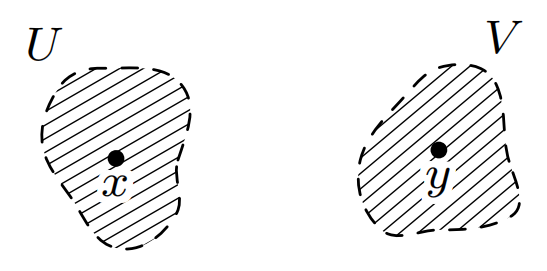
\includegraphics[scale=0.5]{HausdorffAxiom}
		\caption[Hausdorff space]{Hausdorff space}
		\label{fig:hausdorffaxiom}
	\end{figure}
	\begin{thm}
		Any metric space is Hausdorff.
	\end{thm}
	\begin{thm}
		A space $X$ is Hausdorff iff 
		\[\forall x\in X [\set{x}=\bigcap_{U\ni x}\closure{U}],\]
		where $\closure{U}$ is the closure of $U$.
	\end{thm}
	\begin{thm}
		In a Hausdorff space any sequence has at most one limit.
	\end{thm}
	\begin{def*}[hereditary properties]
		A topological property is \textbf{hereditary}
		if it carries over from a space to its
		subspaces, \ie, if a space $X$ has this property,
		then each subspace of $X$ also
		has it.
	\end{def*}
	\begin{thm}
		The property of being a Hausdorff space is hereditary,
		\ie, each subspace of a Hausdorff space is Hausdorff.
	\end{thm}
	\paragraph{Topological Distinguishability and Separated Sets}
	
	\begin{def*}[topological distinguishability]
		Given a topological space $(X,\tau)$ and $x,y\in X$,
		below statements are equivalent:
		\begin{itemize}
			\item $x$ and $y$ are \textbf{topologically distinguishable},
			\item $x$ and $y$ do not have the same open neighbourhoods, 
			\item at least one of them has a neighbourhood that is not a neighbourhood of the other,
			\item there is an open set that one point belongs to but the other point does not:
			%\[\exists U\in\tau[(x\in U\land y\notin U) \lor (y\in U\land x\notin U)] .\]
			\[\exists U\in\tau[x\in U\iff y\notin U] .\]
		\end{itemize}
		\begin{figure}[H]
			\centering
			%
\includegraphics[scale=0.2]{topologically_distinguishable}
			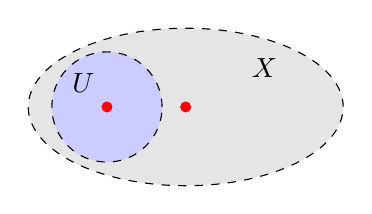
\begin{tikzpicture}
				\draw[dashed,fill=gray!20] (1,0) ellipse (2 and 1) (2.0,0.5) node [text=black] {$X$};
				\draw[dashed,fill=blue!20] (0,0) circle (.7) (-.3,0.3) node [text=black] {$U$};
				\fill[red] (0,0) circle (2pt) (1,0) circle (2pt);
			\end{tikzpicture}
			\caption{Topologically distinguishable points}
			\label{fig:topologically_distinguishable}
		\end{figure}
	\end{def*}

	\begin{def*}[separated sets]
		Given a topological space $(X,\tau)$ and $A,B\subseteq X$,
		they are (from weaker to stronger condition)
		\begin{enumerate}
			\item \textbf{disjoint} iff \[A\cap B=\emptyset; \]
			\begin{figure}[H]
				\centering
				%
\includegraphics[scale=0.2]{topologically_distinguishable}
				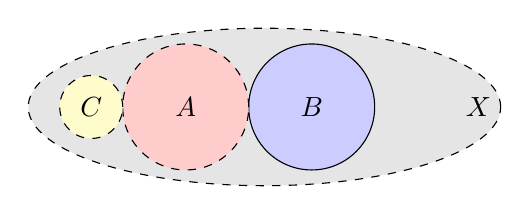
\begin{tikzpicture}
					\draw[dashed,fill=gray!20] (0,0) ellipse (3 and 1) (3.0,0.0) node [text=black,left] {$X$};
					%\draw[fill=blue!20] (.8,0) circle (.8) (.8,0) node [text=black] {$B$};
					%\draw[dashed,fill=red!20] (-.8,0) circle (.8) (-.8,0) node [text=black] {$A$};
					%%\draw[dashed,fill=gray!50] (-.8,0) circle (.8) (-.8,0) node [text=black] {$A$};
					\draw[fill=blue!20] (.6,0) circle (.8) (.6,0) node [text=black] {$B$};
					\draw[dashed,fill=red!20] (-1,0) circle (.8) (-1,0) node [text=black] {$A$};
					\draw[dashed,fill=yellow!20] (-2.2,0) circle (.4) (-2.2,0) node [text=black] {$C$};
				\end{tikzpicture}
				\caption{Disjoint sets}
				\label{fig:disjoint_sets}
			\end{figure}
			\item \textbf{separated} iff \[A \cap \closure{B}= B\cap \closure{A}=\emptyset; \]
			\begin{figure}[H]
				\centering
				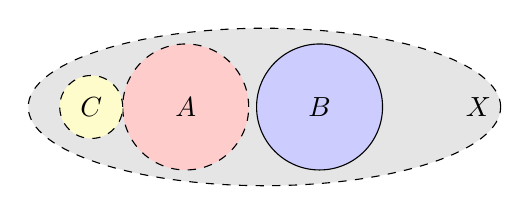
\begin{tikzpicture}
					%\draw[dashed,fill=blue!20] (.8,0) circle (.8) (.8,0) node [text=black] {$B$};
					%\draw[dashed,fill=gray!50] (-.8,0) circle (.8) (-.8,0) node [text=black] {$A$};
					%\draw[dashed,fill=gray!20] (0,0) ellipse (3 and 1) (3.0,0.0) node [text=black,left] {$X$};
					%\draw[fill=blue!20] (.85,0) circle (.8) (.85,0) node [text=black] {$B$};
					%\draw[dashed,fill=red!20] (-.85,0) circle (.8) (-.85,0) node [text=black] {$A$};
					%\draw[dashed,fill=red!20] (-.85,0) circle (.2) (-.85,0) node [text=black] {$C$};
					\draw[dashed,fill=gray!20] (0,0) ellipse (3 and 1) (3.0,0.0) node [text=black,left] {$X$};
					\draw[fill=blue!20] (.7,0) circle (.8) (.7,0) node [text=black] {$B$};
					\draw[dashed,fill=red!20] (-1,0) circle (.8) (-1,0) node [text=black] {$A$};
					\draw[dashed,fill=yellow!20] (-2.2,0) circle (.4) (-2.2,0) node [text=black] {$C$};
				\end{tikzpicture}
				\caption{Separated sets}
				\label{fig:separated_sets}
			\end{figure}
			\item \textbf{separated by neighbourhoods} iff there are (open) neighbourhoods $U$ of $A$ and $V$ of $B$
			such that $U$ and $V$ are disjoint:
			\[ \exists U,V\in\tau[A\subseteq U\land B\subseteq V\land U\cap V=\emptyset]. \]
			
			\begin{figure}[H]
				\centering
				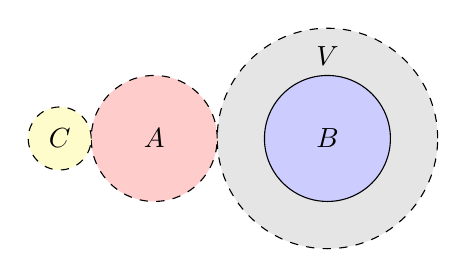
\begin{tikzpicture}
					\draw[dashed,fill=gray!20] (1.2,0) circle (1.4) (1.2,.8) node [text=black,above] {$V$};
					\draw[fill=blue!20] (1.2,0) circle (.8) (1.2,0) node [text=black] {$B$};
					\draw[dashed,fill=red!20] (-1,0) circle (.8) (-1,0) node [text=black] {$A$};
					\draw[dashed,fill=yellow!20] (-2.2,0) circle (.4) (-2.2,0) node [text=black] {$C$};
				\end{tikzpicture}
				\caption{Separated by neighbourhoods}
				\label{fig:separated_by_neighbourhoods}
			\end{figure}
			\item \textbf{separated by closed neighbourhoods} iff there is a closed neighbourhood $U$ of $A$
			and a closed neighbourhood $V$ of $B$ such that $U$ and $V$ are disjoint:
			\[
			\begin{aligned}
				\exists U\exists V\exists U_o, V_o\in \tau[&X\setminus U\in \tau\land X\setminus V\in \tau\\
				&\land A\subseteq U_o\subseteq U\land B\subseteq V_o\subseteq V\land
				U\cap V=\emptyset ],\\ 
			\end{aligned}\]
			or equivalently
			\[\begin{aligned}
				 \exists U_o,V_o,U^c,V^c\in \tau[&A\subseteq U_o\land U_o\cap U^c=\emptyset 
				\land B\subseteq V_o\land V_o\cap V^c=\emptyset\\
				&\land U^c\cup V^c = X ],\\
			\end{aligned} \]
			which, geometrically, implies that there is a ``wall'' separating open neighbourhoods $U_o$ and $V_o$.
			\begin{figure}[H]
				\centering
				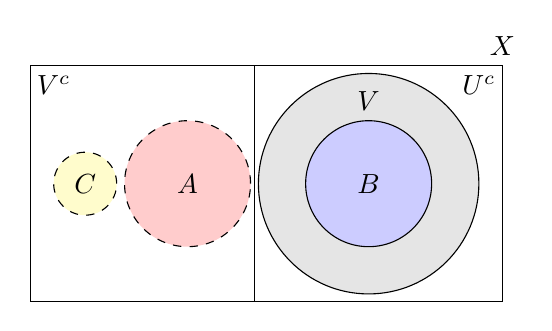
\begin{tikzpicture}
					\draw 
					(-3,-1.5) rectangle (-.15,1.5)
					(-3,-1.5) rectangle (3,1.5) node [text=black,above] {$X$}
					(-2.7,1.5) node [text=black,below] {$V^c$}
					 (2.7,1.5) node [text=black,below] {$U^c$};
					\draw[fill=gray!20] (1.3,0) circle (1.4) (1.3,.8) node [text=black,above] {$V$};
					\draw[fill=blue!20] (1.3,0) circle (.8) (1.3,0) node [text=black] {$B$};
					\draw[dashed,fill=red!20] (-1,0) circle (.8) (-1,0) node [text=black] {$A$};
					\draw[dashed,fill=yellow!20] (-2.3,0) circle (.4) (-2.3,0) node [text=black] {$C$};
				\end{tikzpicture}
				\caption{Separated by closed neighbourhoods}
				\label{fig:separated_by_closed_neighbourhoods}
			\end{figure}
			It can also be simplified using closure:
			\[ \exists U,V\in\tau[A\subseteq U\land B\subseteq V\land \closure{U}\cap\closure{ V}=\emptyset]. \]
		
			\item
			\textbf{separated by a function} iff there exists a \textit{continuous} function $f\colon X\to \re$ such that $f(A) = \set{0}$
			and $f(B) = \set{1}$. 
			\begin{figure}[H]
				\centering
				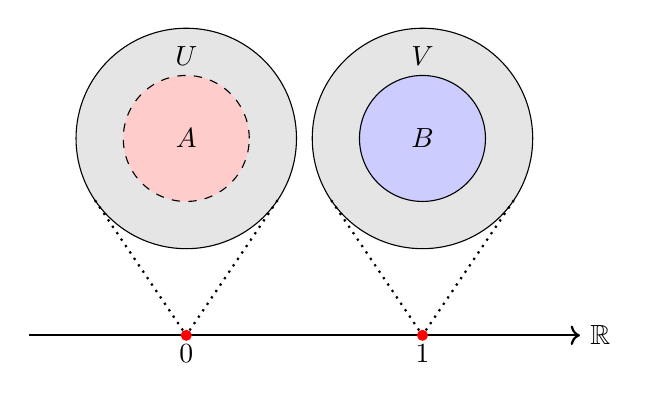
\begin{tikzpicture}
					\def\rb{1.4};
					\def\rs{0.8};
					\def\pos{1.5};
					\def\axis{-2.5};
					\def\xaxis{3.5};
					\pgfmathsetmacro\dx{\rb/(-\axis)*sqrt(\axis*\axis-\rb*\rb)};
					\pgfmathsetmacro\y{-sqrt(\rb*\rb-\dx*\dx)};
					\draw[fill=gray!20] ({\pos},0) circle (\rb) ({\pos},\rs) node [text=black,above] {$V$};
					\draw[fill=gray!20] ({-\pos},0) circle (\rb) ({-\pos},\rs) node [text=black,above] {$U$};
					\draw[fill=blue!20] ({\pos},0) circle (\rs) node [text=black] {$B$};
					\draw[dashed,fill=red!20] ({-\pos},0) circle (\rs) node [text=black] {$A$};
					%\fill[red] (\dx,\axis) circle (2pt);
					\draw[dotted,thick]
					({-\dx-\pos},{\y}) -- ({-\pos},\axis)
					({\dx-\pos},{\y}) -- ({-\pos},\axis)
					({-\dx+\pos},{\y}) -- ({\pos},\axis)
					({\dx+\pos},{\y}) -- ({\pos},\axis);
					\draw[thick,->] ({-\xaxis},\axis) -- ({\xaxis},\axis) node [text=black,right] {$\re$};
					\fill[red] ({-\pos},\axis) circle (2pt) node [text=black,below] {$0$}
					           ({\pos},\axis) circle (2pt) node [text=black,below] {$1$};
				\end{tikzpicture}
				\caption{Separated by a function ($U$ and $V$ are zero sets)}
				\label{fig:separated_by_function}
			\end{figure}
			\item
				\textbf{precisely separated by a function} if there exists a continuous function $f\colon X\to\re$
				such that
				$f^{-1}(\set{0}) = A$ and $f^{-1}(\set{1}) = B$. 
			\begin{figure}[H]
			\centering
			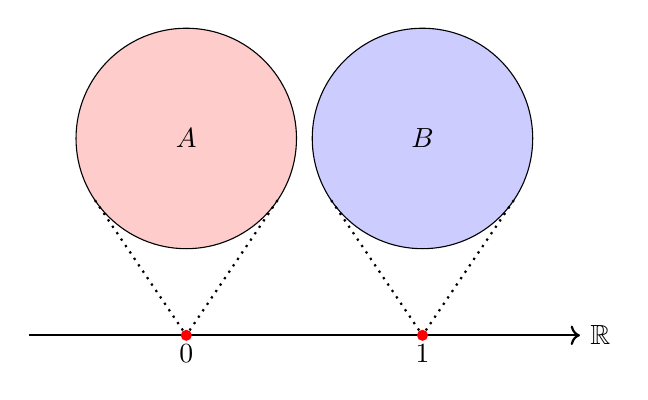
\begin{tikzpicture}
				\def\rb{1.4};
				\def\pos{1.5};
				\def\axis{-2.5};
				\def\xaxis{3.5};
				\pgfmathsetmacro\dx{\rb/(-\axis)*sqrt(\axis*\axis-\rb*\rb)};
				\pgfmathsetmacro\y{-sqrt(\rb*\rb-\dx*\dx)};
				\draw[fill=blue!20] ({\pos},0) circle (\rb) node [text=black] {$B$};
				\draw[fill=red!20] ({-\pos},0) circle (\rb) node [text=black] {$A$};
				%\fill[red] (\dx,\axis) circle (2pt);
				\draw[dotted,thick]
				({-\dx-\pos},{\y}) -- ({-\pos},\axis)
				({\dx-\pos},{\y}) -- ({-\pos},\axis)
				({-\dx+\pos},{\y}) -- ({\pos},\axis)
				({\dx+\pos},{\y}) -- ({\pos},\axis);
				\draw[thick,->] ({-\xaxis},\axis) -- ({\xaxis},\axis) node [text=black,right] {$\re$};
				\fill[red] ({-\pos},\axis) circle (2pt) node [text=black,below] {$0$}
				({\pos},\axis) circle (2pt) node [text=black,below] {$1$};
			\end{tikzpicture}
			\caption{Precisely separated by a function ($A$ and $B$ are zero sets)}
			\label{fig:precisely_separated_by_function}
			\end{figure}
		\end{enumerate}
	\end{def*}
	\begin{def*}[separated points]
		Given a topological space $(X,\tau)$ and $x,y\in X$,
		below statements are equivalent:
		\begin{itemize}
			\item $x$ and $y$ are \textbf{separated},
			\item $\set{x}$ and $\set{y}$ are separated,
			\item each of them has a neighbourhood that is not a neighbourhood of the other,
			\item \[\exists U_x,V_y\in\tau[x\in U_x\land x\notin V_y\land y\in V_y\land y\notin U_x]. \]
		\end{itemize}
	
		\begin{figure}[H]
			\centering
			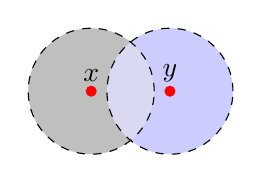
\begin{tikzpicture}
				\scope
				\fill[blue!20] (.5,0) circle (.8);
				\fill[gray!50] (-.5,0) circle (.8);
				\endscope
				\scope
				\clip (.5,0) circle (.8);
				\fill[gray!50!blue!20] (-.5,0) circle (.8);
				\endscope
				\draw[dashed] (.5,0) circle (.8);
				\draw[dashed] (-.5,0) circle (.8);
				\fill[red] (-.5,0) circle (2pt) (-.5,0) node [text=black,above] {$x$};
				\fill[red] (.5,0) circle (2pt) (.5,0) node [text=black,above] {$y$};
			\end{tikzpicture}
			\caption{Separated points}
			\label{fig:separated_points}
		\end{figure}
	\end{def*}
	\begin{rem*}
		\begin{eqlong}
			\set{x}\cap \closure{\set{y}} =\emptyset \iff x\notin\closure{\set{y}}\iff
						U_x\subseteq X\setminus\closure{\set{y}}\iff y\notin U_x\in\tau.
		\end{eqlong}
	%$,V_y=X\setminus\closure{\set{x}}.$
	\end{rem*}
	\begin{prop}
		% Two %topologically distinguishable
		%  points are not separated, if and only if
		% each neighbourhood of one point is
		% contained in a neighbourhood of the other point.
		Two	points $x,y$ are not separated, iff
		for each neighbourhood $U_x$ of $x$ and each neighbourhood $V_y$ of $y$,
		either one of them is a neighbourhood of both points.
	\end{prop}
	\begin{proof}
		%Given a topological space $X,\tau$ and two topologically distinguishable points $x,y\in X$.
		%Without loss of generality, let's assume \[\exists U_x\in\tau[x\in U_x\land y\notin U_x] .\]
		%
		%Since $y\in X\in \tau$, therefore
		%\[\exists V_y\in \tau[y\in V_y]. \]
		%
		%Since They are not separated, then
		%\[ \forall U_x,V_y\in\tau[x\notin U_x\lor x\in V_y\lor y\notin V_y\lor y\in U_x], \]
		%which indicates
		%\[ \forall U_x,V_y\in\tau[(x\in U_x\land y\notin U_x \land y\in V_y) \implies x\in V_y], \]
		
		Given a topological space $(X,\tau)$ and two points $x,y\in X$ that are not separated,
		from definition of separated points, we get
		\[ \forall U_x,V_y\in\tau[x\notin U_x\lor x\in V_y\lor y\notin V_y\lor y\in U_x], \]
		which is equivalent to
		\[ \forall U_x,V_y\in\tau[(x\in U_x\land y\in V_y) \implies (x\in V_y\lor y\in U_x)]. \]
				
		%Since the formula is symmetric,
		%without loss of generality, let's assume 
		%\[ \forall U_x,V_y\in\tau[(x\in U_x\land y\in V_y) \implies (x\in V_y)]. \]
		%
		%Since $\forall U_x,V_y\in\tau[\exists V'_y\in\tau(V'_y=U_x\cup V_y)]$
		%
		%
		%Since $y\in X\in \tau$, therefore
		%\[\exists V_y\in \tau[y\in V_y]. \]
	\end{proof}
	\paragraph{Hierarchy of Separation Axioms}
	\subparagraph{Definition}
	\begin{def*}[separation axioms without T0]
		Given a topological space $X$,
		
		
		\begin{itemize}
			
			\item $X$ is $R_0$, or \textbf{symmetric}, if any two topologically distinguishable points in $X$ are separated.
			
			\item $X$ is $R_1$, or \textbf{preregular}, if any two topologically distinguishable points in $X$ are separated by neighbourhoods.
			
			\item $X$ is \textbf{regular} if any closed set $F\subseteq X$ and any point $x\in X\setminus F$
			are separated by neighbourhoods.
			
			\item 
			$X$ is \textbf{completely regular} if any closed set $F\subseteq X$ and any point $x\in X\setminus F$ are separated by a continuous function.
			
			\item
			$X$ is \textbf{normal} if any two disjoint closed subsets of $X$ are separated by neighbourhoods.
			
			\item
			$X$ is \textbf{normal regular} if it is both $R_0$ and normal. Every normal regular space is regular.
			
			\item $X$ is \textbf{completely normal} if any two separated sets are separated by neighbourhoods.
			\item $X$ is a $G_\delta$ space if every closed set is a $G_\delta$ set.
			\item $X$ is \textbf{perfectly normal} if any two disjoint closed sets are precisely separated by a continuous function.
		\end{itemize}
	\end{def*}

	\begin{rem*}
		For perfectly normal space,
		see this for more equivalent definition: \ref{thmPerfectlyNormal}.
	\end{rem*}
		
	\begin{def*}[separation axioms]
		Given a topological space $(X,\tau)$,
		\begin{itemize}
			\item $X$ is $T_0$, or \textbf{Kolmogorov}, if any two distinct points in $X$ are topologically distinguishable:
			\[\forall x,y\in X [x\ne y \implies\exists U\in\tau (x\in U\iff y\notin U)] .\]
			\item $X$ is $T_1$, or \textbf{accessible}, if any two distinct points in $X$ are separated. Equivalently, every single-point set is a closed set.
			\item $X$ is \textbf{Hausdorff}, or $T_2$, if any two distinct points in $X$ are separated by neighbourhoods.
			\item $X$ is $T_{2\frac{1}{2}}$, or \textbf{Urysohn}, if any two distinct points in $X$ are separated by closed neighbourhoods.
			\item $X$ is \textbf{completely Hausdorff}, or completely $T_2$, if any two distinct points in X are separated by a continuous function.
			\item $X$ is \textbf{regular Hausdorff}, or $T_3$, if it is both $T_0$ and regular.
			\item $X$ is \textbf{Tychonoff}, or $T_{3\frac{1}{2}}$, if it is both $T_0$ and completely regular.
			\item $X$ is \textbf{normal Hausdorff}, or $T_4$, if it is both $T_1$ and normal.
			
			\item $X$ is \textbf{completely normal Hausdorff}, or $T_5$, if it is both completely normal and $T_1$.

			\item $X$ is \textbf{perfectly normal Hausdorff}, or $T_6$, if it is both perfectly normal and $T_1$.
		\end{itemize}
	\end{def*}
	\subparagraph{Properties}
	\begin{lem}
		A topological space $(X,\tau)$ is not $T_0$ iff
		\[\exists x,y\in X[x\ne y\land \forall U\in \tau (X\in U\iff y\in U)] .\]
	\end{lem}
	\begin{prop}
		For any nonempty $T_0$ topological space $(X,\tau)$ and $y\notin X$,
		one can always construct a non-$T_0$ space $(X\cup\set{y},\tau')$.
	\end{prop}
	\begin{proof}
		Pick an arbitrary $x\in X$ and replace each of the open set $U\ni x$ with
		$U\cup\set{y}$. Easy to prove the new collection of open sets is a topology on $X\cup\set{y}$
		in which $x$ and $y$ are not topologically distinguishable:
	\end{proof}
	
	\begin{thm}
		Given a topological space $(X,\tau)$, the following statements are equivalent:
		\begin{itemize}
			\item $X$ is regular topological space,
			\item any closed set $F\subseteq X$ and any point $x\in X\setminus F\in\tau$ 
			are separated by \textbf{closed} neighbourhoods,
			\item given any point $x\in X$ and neighbourhood $G$ of $x$, there is a closed neighbourhood $E$ of $x$ that is a subset of $G$,
			\item the closed neighbourhoods of each point in a topological space form a local base at that point.
		\end{itemize}
	\end{thm}
	

	\begin{thm}
		A topological space is normal if and only if any two disjoint closed sets can be separated by \textbf{a continuous function}.
	\end{thm}

	\begin{thm}
		Given a topological space $(X,\tau)$, the following statements are equivalent:
		\begin{itemize}
			\item $X$ is completely normal, \ie, every two separated sets can be separated by neighbourhoods,
			\item every subspace of $X$ with subspace topology is a normal space,
			\item every open subset of $X$ is normal with the subspace topology.
		\end{itemize}
	\end{thm}
	
	\subparagraph{Visualization of Hierarchy}
	
	See \ref{fig:separation_axiom_hierarchy}.
	
	\begin{figure}[H]
		\centering
		%\begin{tikzpicture}%[baseline= (a).base]
		%	\matrix[anchor=center,column sep={3cm,between origins},row sep={2cm,between origins}] {
		%		&\node {d};&\node {PNR/T\textsubscript{6}};\\
		%		&\node {PN/PNT\textsubscript{0}}; && \node {CNR/T\textsubscript{5}};\\
		%		\node {$G_\delta/\bullet$}; && \node {CN/CNT\textsubscript{0}}; && \node {NR/T\textsubscript{4}};\\
		%		\node {d};&\node {d};&\node {d};&\node {N/NT\textsubscript{0}};&&\node {CR/T${}_{3\frac{1}{2}}$};\\
		%		\node {d};&\node {d};&\node {d};&\node {d};&\node {d};&\node {d};&\node {d};&\node {d};\\
		%	};
		%	%\node
		%	%(a) at (0,0){PNR/T\textsubscript{6}}
		%	%(-1,-1){PN/PNT\textsubscript{0}}
		%	%(-1,-1){PN/PNT\textsubscript{0}}
		%	%;
		%
		%\end{tikzpicture}
	
		\begin{tikzpicture}	
			\node[scale=.8] (a) at (0,0){
				\begin{tikzcd}[anchor=center,
					column sep={1.0cm,between origins},
					row sep={1.2cm,between origins}]
					&&\mathrm{PNR}/\rmT_6\ar[rd,dash]\ar[ld,dash]&&&&&&\\
					&\mathrm{PN}/\mathrm{PNT}_0\ar[rd,dash]\ar[ld,dash]&&\mathrm{CNR}/\rmT_5\ar[rd,dash]\ar[ld,dash]\\
					\mathrm{G}_\delta/\bullet&&\mathrm{CN}/\mathrm{CNT}_0\ar[rd,dash]&&\mathrm{NR}/\rmT_4\ar[rd,dash]\ar[ld,dash]\\
					&&&\mathrm{N}/\mathrm{NT}_0\ar[dddddd,dash]&&\mathrm{CR}/\rmT_{3\frac{1}{2}}\ar[rd,dash]\\
					&&&&&&\bullet/\bullet\ar[rd,dash]\ar[ld,dash]\\
					&&&&&\bullet/\mathrm{CT}_2\ar[rd,dash]&&\rmR/\rmT_3\ar[ld,dash]\\
					&&&&&&\bullet/\rmT_{2\frac{1}{2}}\ar[ld,dash]&&\mathrm{SR}/\bullet\ar[from=ul,dash] \\
					&&&&&\rmR_1/\rmT_2\ar[ld,dash]\\
					&&&&\rmR_0/\rmT_1\ar[ld,dash]\\
					&&&-/\rmT_0\\
				\end{tikzcd}
			};
 		\end{tikzpicture}
		
		%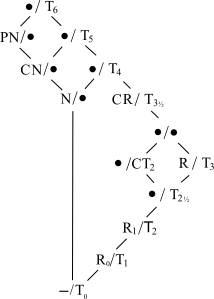
\includegraphics[scale=0.6]{Separation_axioms}
		\caption{Hierarchy of separation axioms (SR=semiregular, iff, regular open sets (sets equal to the interiors of their closures) form a base).\\
			Upper $\implies$ lower.\\
			Left $+T_0 \iff$ Right.\\
			*N $+T_1 \iff$ T*.\\
			*N $+R_0\iff$ *NR.\\
			N $+G_\delta\iff$ PN.
			% Upper axioms imply lower axioms. Right-to-the-slash axioms
			%imply the ones to the left (no $T_0$ version).
			%Left + $T_0$ iff Right axiom
			%Normal + $T_1$ iff $T_x$
			%NR iff normal+R0
		}
		\label{fig:separation_axiom_hierarchy}
	\end{figure}
	
	\subparagraph{Visualization of Separation Axioms}
	
	See \ref{fig:visualized_separation_axiom}.
	
	\begin{figure}[H]
		\centering
		
		\begin{subfigure}{0.45\textwidth}
			\centering
			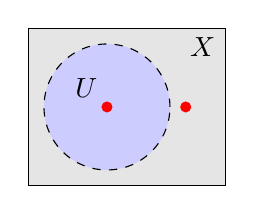
\begin{tikzpicture}[remember picture]
				\draw[fill=gray!20]
				(-1,-1) rectangle (1.5,1) node [text=black, below left] {$X$};
				\draw[dashed,fill=blue!20] (0,0) circle (.8) node [text=black, above left] {$U$};
				\fill[red] (0,0) circle (2pt) (1,0) circle (2pt);
			\end{tikzpicture}
			\caption{$T_0$ space}
		\end{subfigure}%
		\begin{subfigure}{0.45\textwidth}
			\centering
			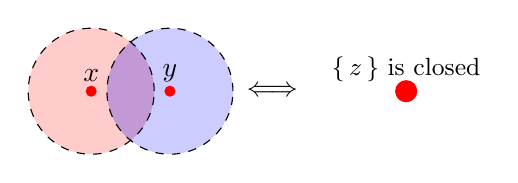
\begin{tikzpicture}[remember picture]
				\scope
				\fill[blue!20] (.5,0) circle (.8);
				\fill[red!20] (-.5,0) circle (.8);
				\endscope
				\scope
				\clip (.5,0) circle (.8);
				\fill[red!40!blue!40] (-.5,0) circle (.8);
				\endscope
				\draw[dashed] (.5,0) circle (.8);
				\draw[dashed] (-.5,0) circle (.8);
				\fill[red] (-.5,0) circle (2pt) node [text=black,above] {$x$};
				\fill[red] (.5,0) circle (2pt) node [text=black,above] {$y$};
				\node (A) at (1.8,0) {$\iff$};
				\fill[red] (3.5,0) circle (4pt) node [text={black},above] {\small $\set{z}$ is closed};
			\end{tikzpicture}
			\caption{$T_1$ space}
		\end{subfigure}

		\begin{subfigure}{0.45\textwidth}
			\centering
			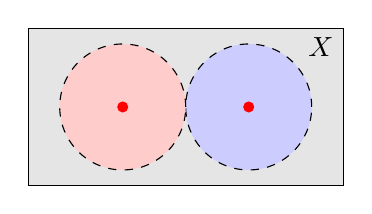
\begin{tikzpicture}[remember picture]
				\draw[fill=gray!20]
				(-2,-1) rectangle (2,1) node [text=black, below left] {$X$};
				\draw[dashed,fill=blue!20] (.8,0) circle (.8);
				\draw[dashed,fill=red!20] (-.8,0) circle (.8);
				\fill[red] (-.8,0) circle (2pt) (.8,0) circle (2pt);
			\end{tikzpicture}
			\caption{$T_2$ space}
		\end{subfigure}%
		\begin{subfigure}{0.45\textwidth}
			\centering
			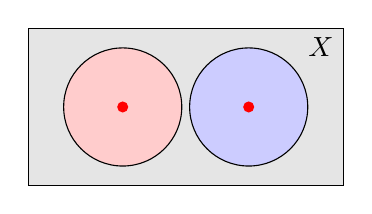
\begin{tikzpicture}[remember picture]
				\draw[fill=gray!20]
				(-2,-1) rectangle (2,1) node [text=black, below left] {$X$};
				\draw[fill=blue!20] (.8,0) circle (.75);
				\draw[fill=red!20] (-.8,0) circle (.75);
				\fill[red] (-.8,0) circle (2pt) (.8,0) circle (2pt);
			\end{tikzpicture}
			\caption{$T_{2\frac{1}{2}}$ space}
		\end{subfigure}
	
		\begin{subfigure}{0.45\textwidth}
			\centering
			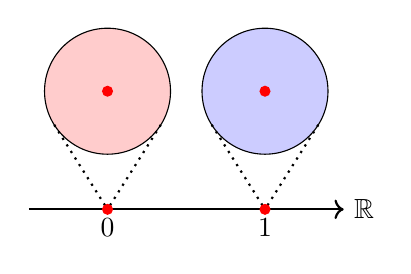
\begin{tikzpicture}[remember picture]
				\def\rb{0.8};
				\def\pos{1.0};
				\def\axis{-1.5};
				\def\xaxis{2.0};
				\pgfmathsetmacro\dx{\rb/(-\axis)*sqrt(\axis*\axis-\rb*\rb)};
				\pgfmathsetmacro\y{-sqrt(\rb*\rb-\dx*\dx)};
				\draw[fill=blue!20] ({\pos},0) circle (\rb);
				\draw[fill=red!20] ({-\pos},0) circle (\rb);
				\fill[red] ({-\pos},0) circle (2pt) ({\pos},0) circle (2pt);
				\draw[dotted,thick]
				({-\dx-\pos},{\y}) -- ({-\pos},\axis)
				({\dx-\pos},{\y}) -- ({-\pos},\axis)
				({-\dx+\pos},{\y}) -- ({\pos},\axis)
				({\dx+\pos},{\y}) -- ({\pos},\axis);
				\draw[thick,->] ({-\xaxis},\axis) -- ({\xaxis},\axis) node [text=black,right] {$\re$};
				\fill[red] ({-\pos},\axis) circle (2pt) node [text=black,below] {$0$}
				({\pos},\axis) circle (2pt) node [text=black,below] {$1$};
			\end{tikzpicture}
			\caption{Completely $T_2$ space}
		\end{subfigure}%
		\begin{subfigure}{0.45\textwidth}
			\centering
			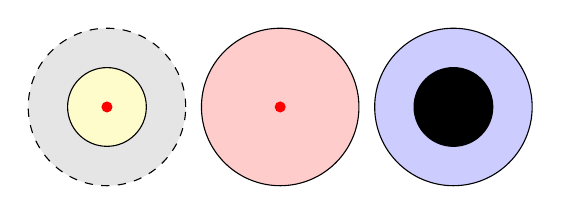
\begin{tikzpicture}[remember picture]
				\draw[dashed,fill=gray!20] (0,0) circle (1.0);
				\draw[fill=yellow!20] (0,0) circle (.5);
				\fill[red] (0,0) circle (2pt);
				\draw[fill=red!20] (2.2,0) circle (1.0);
				\fill[red] (2.2,0) circle (2pt);
				\draw[fill=blue!20] (4.4,0) circle (1.0);
				\draw[fill=black] (4.4,0) circle (0.5);
			\end{tikzpicture}
			\caption{Regular space}
		\end{subfigure}

		\begin{subfigure}{0.45\textwidth}
			\centering
			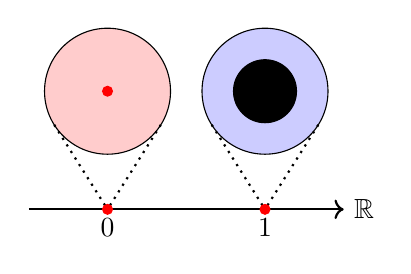
\begin{tikzpicture}[remember picture]
				\def\rb{0.8};
				\def\rs{0.4};
				\def\pos{1.0};
				\def\axis{-1.5};
				\def\xaxis{2.0};
				\pgfmathsetmacro\dx{\rb/(-\axis)*sqrt(\axis*\axis-\rb*\rb)};
				\pgfmathsetmacro\y{-sqrt(\rb*\rb-\dx*\dx)};
				\draw[fill=blue!20] ({\pos},0) circle (\rb);
				\draw[fill=black] ({\pos},0) circle (\rs);
				\draw[fill=red!20] ({-\pos},0) circle (\rb);
				\fill[red] ({-\pos},0) circle (2pt);
				\draw[dotted,thick]
				({-\dx-\pos},{\y}) -- ({-\pos},\axis)
				({\dx-\pos},{\y}) -- ({-\pos},\axis)
				({-\dx+\pos},{\y}) -- ({\pos},\axis)
				({\dx+\pos},{\y}) -- ({\pos},\axis);
				\draw[thick,->] ({-\xaxis},\axis) -- ({\xaxis},\axis) node [text=black,right] {$\re$};
				\fill[red] ({-\pos},\axis) circle (2pt) node [text=black,below] {$0$}
				({\pos},\axis) circle (2pt) node [text=black,below] {$1$};
			\end{tikzpicture}
			\caption{Completely regular space}
		\end{subfigure}%
		\begin{subfigure}{0.45\textwidth}
			\centering
			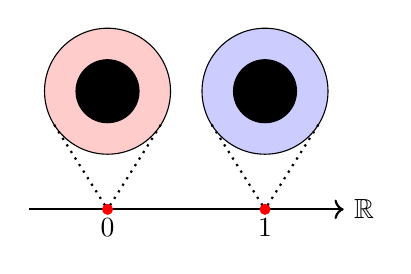
\begin{tikzpicture}[remember picture]
				\def\rb{0.8};
				\def\rs{0.4};
				\def\pos{1.0};
				\def\axis{-1.5};
				\def\xaxis{2.0};
				\pgfmathsetmacro\dx{\rb/(-\axis)*sqrt(\axis*\axis-\rb*\rb)};
				\pgfmathsetmacro\y{-sqrt(\rb*\rb-\dx*\dx)};
				\draw[fill=blue!20] ({\pos},0) circle (\rb);
				\draw[fill=black] ({\pos},0) circle (\rs);
				\draw[fill=red!20] ({-\pos},0) circle (\rb);
				\draw[fill=black] ({-\pos},0) circle (\rs);
				\draw[dotted,thick]
				({-\dx-\pos},{\y}) -- ({-\pos},\axis)
				({\dx-\pos},{\y}) -- ({-\pos},\axis)
				({-\dx+\pos},{\y}) -- ({\pos},\axis)
				({\dx+\pos},{\y}) -- ({\pos},\axis);
				\draw[thick,->] ({-\xaxis},\axis) -- ({\xaxis},\axis) node [text=black,right] {$\re$};
				\fill[red] ({-\pos},\axis) circle (2pt) node [text=black,below] {$0$}
				({\pos},\axis) circle (2pt) node [text=black,below] {$1$};
			\end{tikzpicture}
			\caption{Normal space}
		\end{subfigure}

		\begin{subfigure}{0.45\textwidth}
			\centering
			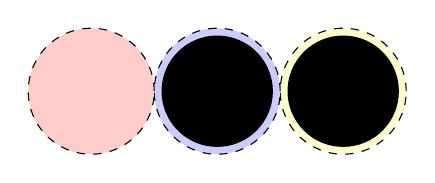
\begin{tikzpicture}[remember picture]
				\draw[dashed,fill=yellow!20] (1.6,0) circle (.8);
				\draw[dashed,fill=blue!20] (0,0) circle (.8);
				\draw[dashed,fill=red!20] (-1.6,0) circle (.8);
				\draw[fill=black] (0,0) circle (.7) (1.6,0) circle (.7);
			\end{tikzpicture}
			\caption{Completely normal space}
		\end{subfigure}%
		\begin{subfigure}{0.45\textwidth}
			\centering
			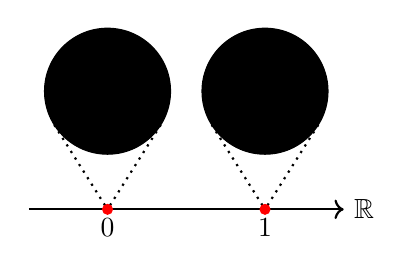
\begin{tikzpicture}[remember picture]
				\def\rb{0.8};
				\def\pos{1.0};
				\def\axis{-1.5};
				\def\xaxis{2.0};
				\pgfmathsetmacro\dx{\rb/(-\axis)*sqrt(\axis*\axis-\rb*\rb)};
				\pgfmathsetmacro\y{-sqrt(\rb*\rb-\dx*\dx)};
				\draw[fill=black] ({\pos},0) circle (\rb) node [text=black] {$B$};
				\draw[fill=black] ({-\pos},0) circle (\rb) node [text=black] {$A$};
				\draw[dotted,thick]
				({-\dx-\pos},{\y}) -- ({-\pos},\axis)
				({\dx-\pos},{\y}) -- ({-\pos},\axis)
				({-\dx+\pos},{\y}) -- ({\pos},\axis)
				({\dx+\pos},{\y}) -- ({\pos},\axis);
				\draw[thick,->] ({-\xaxis},\axis) -- ({\xaxis},\axis) node [text=black,right] {$\re$};
				\fill[red] ({-\pos},\axis) circle (2pt) node [text=black,below] {$0$}
				({\pos},\axis) circle (2pt) node [text=black,below] {$1$};
			\end{tikzpicture}
			\caption{Perfectly normal space}
		\end{subfigure}
		
		%\begin{tabular}{C{.48\textwidth}C{.48\textwidth}}
		%	%%%%%%%%%%%%%%%%%%%%%% 1 %%%%%%%%%%%%%%%%%%%%%%%%%%%%%%%%%%%
		%	\subfigure [Subfigure 1] {
		%		\resizebox{0.4\textwidth}{!}{%
		%			\begin{tikzpicture}
		%				\node;
		%			\end{tikzpicture} 
		%		}
		%	} & 
		%	%%%%%%%%%%%%%%%%%%%%%% 2 %%%%%%%%%%%%%%%%%%%%%%%%%%%%%%%%%%%
		%	\subfigure [Subfigure 2] {
		%		\resizebox{0.4\textwidth}{!}{%
		%			\begin{tikzpicture}[->,>=stealth',shorten >=2pt,node distance=2.0cm,
		%				semithick] % ,scale=.5]
		%				\tikzstyle{every state}=[fill=white,draw=black,text=black,font=\small]
		%				\node[state] (A) [label=above:$N_{f\_1}$]                                          {$1$};
		%				\node[state] (B) [below left  of = A,     label=above:$N_{a1}$]    {$\boldsymbol{2}$};
		%				\node[state] (C) [below right of = A , style={dashed},  label=above:$N_{b1}$]      {$\boldsymbol{3}$};
		%				\node[state] (D) [below right of = C,  label=above:$N_{c_1}$]    {$\boldsymbol{4}$};    
		%				\path (B) edge []       node {} (A)
		%				(C) edge []             node {} (A)
		%				(D) edge []       node {} (C)                               
		%				;               
		%			\end{tikzpicture} 
		%		}
		%	} \\
		%	
		%	%%%%%%%%%%%%%%%%%%%%%% 3 %%%%%%%%%%%%%%%%%%%%%%%%%%%%%%%%%%%
		%	\subfigure [Subfigure 3] {
		%		\resizebox{0.4\textwidth}{!}{%
		%			\begin{tikzpicture}[->,>=stealth',shorten >=2pt,node distance=2.0cm,
		%				semithick] %,scale=.5]
		%				\tikzstyle{every state}=[fill=white,draw=black,text=black,font=\small]
		%				\node[state] (A) [                     label=above:$N_{f\_1}$, , style={dashed}]                                           {$1$};
		%				\node[state] (B) [below left  of = A,  label=above:$N_{a1}$]   {$\boldsymbol{2}$};
		%				\node[state] (C) [below right of = A,  label=above:$N_{b1}$]   {$\boldsymbol{3}$};
		%				\node[state] (D) [below right of = C,  label=above:$N_{c_1}$]    {$\boldsymbol{4}$};    
		%				\path (B) edge []       node {} (A)
		%				(C) edge []             node {} (A)
		%				(D) edge []       node {} (C)                               
		%				;
		%			\end{tikzpicture} 
		%		}
		%	} & 
		%	
		%	%%%%%%%%%%%%%%%%%%%%%% 4 %%%%%%%%%%%%%%%%%%%%%%%%%%%%%%%%%%%
		%	\subfigure [Subfigure 4] {
		%		\resizebox{0.4\textwidth}{!}{%
		%			\begin{tikzpicture}[->,>=stealth',shorten >=2pt,node distance=2.0cm,
		%				semithick] % ,scale=.5]
		%				\tikzstyle{every state}=[fill=white,draw=black,text=black,font=\small]
		%				\node[state] (A) [                                            label=above:$N_{f\_1}$]                                          {$1$};
		%				\node[state] (B) [below left  of = A,     label=above:$N_{a1}$, style={dashed}]    {$\boldsymbol{2}$};
		%				\node[state] (C) [below right of = A ,  label=above:$N_{b1}$, style={dashed}]      {$\boldsymbol{3}$};
		%				\node[state] (D) [below right of = C,   label=above:$N_{c_1}$]   {$\boldsymbol{4}$};    
		%				\path (B) edge []       node {} (A)
		%				(C) edge []             node {} (A)
		%				(D) edge []       node {} (C)                               
		%				;
		%			\end{tikzpicture} 
		%		}
		%	} \\
		%\end{tabular}
		
		\caption{Visualized separation axiom.}
		\label{fig:visualized_separation_axiom}
	\end{figure}
	
	More visualization:
	\href{https://christopherolah.wordpress.com/2010/08/14/separation-axiom-visualisations/}{1}
	,
	\href{https://publications.chitkara.edu.in/a-class-of-separation-axioms-in-generalized-topology/}{2}.
	
	
	%\begin{thm}
	%	A topological space is Hausdorff if and only if it is both $T_0$ (Kolmogorov) and $R_1$ (preregular).
	%	Every Hausdorff space is also $T_1$ (accessible) and $R_0$ (symmetric).
	%\end{thm}
	
	
	\paragraph{Metrizable Spaces}
	
	\subparagraph{Definition}
	\begin{def*}[metrizable space]
		A \textbf{metrizable space} is a topological space that is homeomorphic to a metric space.
	\end{def*}
	\begin{rem*}
		Equivalently, a topological space $(X,\tau)$
		is said to be metrizable if there is a metric $d\colon X\times X\to \re_0^+$
		such that the topology induced by $d$ is $\tau$.
	\end{rem*}

	\subparagraph{Necessary Condition: $T_6$}

	\begin{thm}
		All metrizable spaces are perfectly normal Hausdorff ($T_6$).
	\end{thm}
	\begin{rem*}
		See \href{https://math.stackexchange.com/questions/73609/is-a-metric-space-perfectly-normal}{this thread} for details.
	\end{rem*}

	\begin{def*}[Gdelta set]
		A \textbf{$G_\delta$ set} is a countable intersection of open sets.
	\end{def*}
	\begin{rem*}
		Given a topology $(X,\tau)$, a set $A\subseteq X$ is $G_\delta$ iff
		\begin{eqlong}
			\exists \sigma \subseteq \tau [\card{\sigma} \le \aleph_0 \land A = \bigcap \sigma].
		\end{eqlong}
	\end{rem*}
	\begin{cor}
		Open sets are $G_\delta$.
	\end{cor}
	\begin{proof}
		By definition.
	\end{proof}
	\begin{thm}
		% Given topological space $(X,\tau)$ and a subset $S\subseteq X$,
		% if there is a continuous function from $S$ to a metric space,
		% then $S$ is $G_\delta$.
		Given a topological space $(X,\tau)$ and
		a function $f$ from $X$ to a metric space,
		the set of points where such a function $f$ is continuous is $G_\delta$.
	\end{thm}

	\begin{thm}
		For any $G_\delta$ subset $A\subseteq\re$, there is a function $f\colon\re\to\re$ that is continuous exactly at the points in $A$, \ie, $f$ is continuous at $x$ iff $x\in A$. 
	\end{thm}
	\begin{cor}
		It is possible for the irrationals to be the set of continuity points of a function,
		but it is impossible to construct a function that is continuous only on the rational numbers.
	\end{cor}
	\begin{def*}[Thomae's function]
		The \textbf{Thomae's function} $f\colon\re\to\re$ is defined as
		\begin{eqlong}
			f(x)=\begin{cases}
				\frac{1}{q}& \exists p\in \inte\exists q\in \nat[\operatorname{gcd}(p,q)=1,x=p/q]\\
				0& \text{otherwise}\\
			\end{cases}.
		\end{eqlong}
	\end{def*}
	\begin{thm}
		The Thomae's function is discontinuous at all rational numbers,
		continuous at all irrational numbers,
		and nowhere differentiable.
	\end{thm}

	\begin{def*}[zero set]
		The \textbf{zero set} of a real-valued function $f\colon X\to\re$ is $f^{-1}(\set{0})$,
	\ie, the inverse image of $\set{0}$ in $X$.
	\end{def*}
	\begin{thm}
		The zero set of every real-valued continuous function is a $G_\delta$ set.
	\end{thm}
	\begin{rem*}
		Since zero set is the intersection of the open sets 
		\[ \set{x\in X|-1/n<f(x)<1/n},\forall n\in \inte^+.\]
	\end{rem*}

	\begin{thm}\label{thmPerfectlyNormal}
		Given a topological space $(X,\tau)$, below are equivalent statements:
		\begin{itemize}
			\item $X$ is perfectly normal;
			\item $X$ is normal and every closed set is a $G_\delta$ set;
			\item Every closed set in $X$ is a zero set of a real-valued continuous function, \ie,
			\[\forall U\in\tau \exists f\in \mathcal{C}^0(X,\re)\forall x\in X[ f(x)=0\iff x\in X\setminus U ], \] 
			where $\mathcal{C}^0(X,\re)$ denotes the class of real-valued continuous functions on $X$.
		\end{itemize}
	\end{thm}
	\begin{rem*}
		See this question:
		\href{https://math.stackexchange.com/questions/72138/why-are-these-two-definitions-of-a-perfectly-normal-space-equivalent}
		{Why are these two definitions of a perfectly normal space equivalent?}
	\end{rem*}

	\begin{cor}
		In a metrizable space, every closed set is a $G_\delta$ set.
	\end{cor}
	\begin{proof}
		Metrizable $\implies$ $T_6$ $\implies$ perfectly normal $\iff$ closed set is zero set.
		
		And zero set is $G_\delta$.
	\end{proof}
	
	
	
	
	
	
	

	\subparagraph{Sufficient Conditions}
	
	\begin{thm}
		Every Hausdorff second-countable regular space is metrizable.
	\end{thm}
	
	\begin{thm}
		A topological space is metrizable if and only if it is regular, Hausdorff and has a $\sigma$-locally finite base. A $\sigma$-locally finite base is a base which is a union of countably many locally finite collections of open sets.
	\end{thm}

	\subsubsection{Compactness}
	\paragraph{Paracompactness and Compactness}
	\begin{def*}[cover]
		A \textbf{cover} of a set $X$ is a collection of sets whose union contains $X$. In symbols, $\mathcal{U}$ is a cover of $X$ iff
		\[X \subseteq \bigcup \mathcal{U}.\]
	\end{def*}

	\begin{def*}[open cover]
		A cover $\mathcal{U}$ of a topological space $(X,\tau)$ is \textbf{open} if all its members are open sets, \ie,
		\[\forall U\in\mathcal{U} [U\in\tau]. \]
	\end{def*}

	\begin{def*}[refinement of a cover]
		A \textbf{refinement of a cover} of a set $X$ is a new cover of the same set
		such that every set in the new cover is a subset of some set in the old cover.
		In symbols, $\mathcal{V}$ is a refinement of the cover $\mathcal{U}$ if and only if,
		\[ X\subseteq\bigcup\mathcal{V} \land \forall V\in\mathcal{V} \exists U\in \mathcal{U}[V\subseteq U]. \]
	\end{def*}

	\begin{def*}[open refinement]
		An \textbf{open refinement of a cover} of a topological space $(X,\tau)$ is a refinement that is also an open cover.
		In symbols, $\mathcal{V}$ is a open refinement of the cover $\mathcal{U}$ if and only if,
		\[ X\subseteq\bigcup\mathcal{V} \land \forall V\in\mathcal{V} [V\in\tau\land\exists U\in \mathcal{U}(V\subseteq U)]. \]
	\end{def*}

	\begin{def*}[locally finite open cover]
		An open cover of a topological space $(X,\tau)$ is \textbf{locally finite}
		if every point of the space has a neighborhood that intersects only finitely many sets in the cover.
		In symbols, $\mathcal{U}$ is locally finite if and only if,
		\[ \forall x\in X \exists V_x\in \tau [x\in V_x\land \card{\set{U\in\mathcal{U} | U\cap V_x\ne\emptyset}}<\aleph_0 ] .\]
	\end{def*}

	\begin{def*}[paracompact space]
		A \textbf{paracompact space} is a topological space in which every open cover has an open refinement that is locally finite.
	\end{def*}
	\begin{rem*}
		A topological space $(X,\tau)$ is paracompact iff
		\begin{center}
			\small
			\setlength{\tabcolsep}{0pt}
			\begin{tabular}{LRL}
				\forall \mathcal{U}\in\power(\tau) [&X=\bigcup \mathcal{U}\implies&\\
				&\exists \mathcal{V}\in\power(\tau)\big(&X=\bigcup \mathcal{V}\land \forall V\in\mathcal{V} \exists U\in \mathcal{U}(V\subseteq U)\\
				&&\land\forall x\in X \exists W_x\in \tau (x\in W_x\land \card{\set{V\in\mathcal{V} | V\cap W_x\ne\emptyset}}\in\nat )\\
				&\big) & ].\\
			\end{tabular}
		\end{center}
	\end{rem*}

	\begin{def*}[subcover]
		A \textbf{subcover} of a cover $\mathcal{C}$ of $X$ is a subset of $\mathcal{C}$ that still covers the set $X$.
	\end{def*}
	\begin{rem*}
		Every subcover is also a refinement, but the opposite is not always true.
	\end{rem*}

	\begin{def*}[compact space]
		A topological space $(X,\tau)$ is \textbf{compact} if
		every open cover of $X$ has a finite subcover, \ie,
		\begin{eqlong}
			\forall \mathcal{U}\subseteq\tau [X=\bigcup \mathcal{U}\implies
			\exists \mathcal{V}\subseteq\mathcal{U}\big(X=\bigcup \mathcal{V}\land \card{\mathcal{V}}\in\nat\big)].
		\end{eqlong}
	\end{def*}
	\begin{rem*}
		Compactness means ``\href{https://blogs.scientificamerican.com/roots-of-unity/what-does-compactness-really-mean/}{small}''
		because you can describe the whole space finitely.
	\end{rem*}

	\paragraph{Other Compactness}
	
	\begin{def*}[point-finite cover]
		A cover $\mathcal{U}$ of $X$ is said to be point-finite if every point of $X$ is contained in only finitely many sets in the cover,
		\ie,
		\[ X\subseteq \bigcup\mathcal{U} \land \forall x \in X[\card{\set{U\in\mathcal{U}|x\in U}}\in\nat] .\]
	\end{def*}
	\begin{rem*}
		A cover is point-finite if it is locally finite, though the converse is not necessarily true.
	\end{rem*}
	
	\begin{def*}[list of compactness]
		A topological space $(X,\tau)$ is
		\begin{itemize}
			\item \textbf{sequentially compact} if every sequence of points in $X$ has a convergent subsequence converging to a point in $X$,
			\item \textbf{limit point compact} if every infinite subset of $X$ has a limit point in $X$,
			\item \textbf{countably compact} if every countable open cover has a finite subcover,
			
			\item \textbf{compact}
			if every open cover has a finite subcover,
			\item \textbf{Lindelöf}
			if every open cover has a countable subcover,
			\item \textbf{metacompact}
			if every open cover has a point-finite open refinement,
			\item \textbf{paracompact}
			if every open cover admits a locally finite open refinement.
		\end{itemize}
	\end{def*}

	\begin{figure}
		\centering
		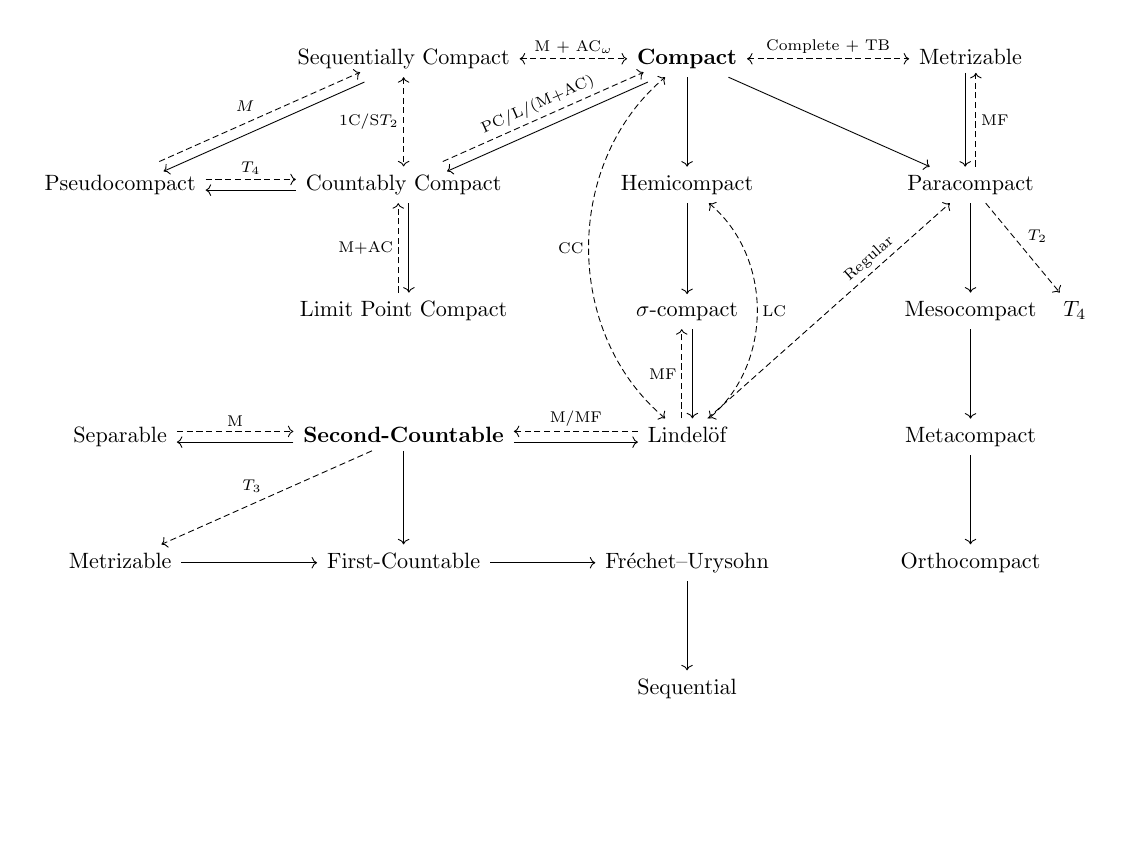
\begin{tikzpicture}	
			\node[scale=.8] (a) at (0,0){
				\begin{tikzcd}[anchor=center,
					column sep={4.5cm,between origins},
					row sep={2.0cm,between origins}
					]
					%%%%%%%%%%%%%%%
					&\text{Sequentially Compact}\ar[d,dashed,leftrightarrow,"\text{1C/S}T_2"']
					\ar[r,leftrightarrow,dashed,"\text{M + AC}{}_\omega"]&\textbf{Compact}\ar[rd]
					\ar[d]
					\ar[ld,shift left]
					\ar[from=ld,dashed,shift left,"\text{PC/L/(M+AC)}"{sloped}']
					&\text{Metrizable} \ar[from=l,leftrightarrow,dashed,"\text{Complete + TB}"]
					\ar[d,shift right]\ar[from=d,dashed,shift right,"\text{MF}"']\\
					%%%%%%%%%%%%%%%
					\text{Pseudocompact} \ar[from=r,shift left]\ar[r,dashed,shift left,"T_4"]\ar[ur,dashed,shift left,"M"]\ar[from=ur,shift left]
					&\text{Countably Compact}\ar[from=d,dashed,shift left,"\text{M+AC}"]\ar[d,shift left]
					&\text{Hemicompact}\ar[d]&\text{Paracompact}\\
					%%%%%%%%%%%%%%%
					&\text{Limit Point Compact}&\sigma\text{-compact}
					\ar[d,shift left]
					\ar[from=d,dashed,shift left,"\text{MF}"]
					&\text{Mesocompact}\ar[from=u]\ar[d] &[-4cm]T_4\ar[from=ul,dashed,"T_2"]\\
					%%%%%%%%%%%%%%%
					\text{Separable}&\textbf{Second-Countable}
					\ar[r,shift right]\ar[from=r,shift right,dashed,"\text{M/MF}"']
					\ar[l,shift left] \ar[from=l,dashed,shift left,"\text{M}"] 
					&\text{Lindelöf}\ar[from=uu,leftrightarrow,bend left=50,dashed,"\text{LC}"]\ar[ruu,dashed,pos=0.7,"\text{Regular}"{sloped}]
					\ar[uuu,leftrightarrow,bend left=50,dashed,"\text{CC}"]
					&\text{Metacompact}\ar[d] \\
					%%%%%%%%%%%%%%%
					\text{Metrizable}\ar[r]\ar[from=ur,dashed,"T_3"']
					&\text{First-Countable}\ar[from=u]&\text{Fréchet--Urysohn}\ar[from=l]&\text{Orthocompact}\\
					%%%%%%%%%%%%%%%
					&&\text{Sequential}\ar[from=u]\\
				\end{tikzcd}
			};
		\end{tikzpicture}
		\caption{Hierarchy of compactness/countability: \\
			solid line = unconditional, dashed line = conditional, \\
			M = metrizable, L = Lindelöf, CC = countably compact, PC = paracompact, LC = locally compact, AC = axiom of choice, TB = totally bounded,
			S$T_2$ = sequential Hausdorff, 1C = first countable, MF = manifold
		}
		\label{fig:compactness}
	\end{figure}
	
	\subsubsection{Countability Axioms}
	
	\begin{def*}[dense]
		Let $A$ and $B$ be two sets in a topological space $(X,\tau)$.
		We call $A$ is \textbf{dense} in $B$ if the one of following equivalent conditions holds
		\begin{itemize}
			\item $B$ is a subset of the closure of $A$, \ie, $B\subseteq\closure{A}$,
			\item points in $B$ are adherent points of $A$, \ie, either in $A$ or a limit point of $A$,
			\item all open neighbourhoods of $x\in B$ intersects with $A$, \ie,
			\[ \forall x\in B\forall U\in\tau[x\in  U \implies A\cap U\ne\emptyset ],\]
			\item all open sets intersecting with $B$ must also intersect $A$, \ie,
			\[ \forall U\in\tau[B\cap  U\ne\emptyset \implies A\cap U\ne\emptyset ].\]
		\end{itemize}
		 $A$ is \textbf{everywhere dense} or simply dense (in $X$) iff $\closure{A} = X$, \ie,
		 \[\forall U\in\tau[U\ne\emptyset\implies A\cap U\ne\emptyset ].\]
	\end{def*}
	\begin{rem*}
		Below shows the equivalence.
		
		\[ \forall x\in B\forall U\in\tau[x\in  U \implies A\cap U\ne\emptyset ],\]
		iff (exchanging $\forall$)
		\[ \forall U\in\tau\forall x\in B[x\in  U \implies A\cap U\ne\emptyset ],\]
		iff (definition of qualified $\forall$ and set intersection)
		\[ \forall U\in\tau\forall x[x\in B \cap  U \implies A\cap U\ne\emptyset ],\]
		iff (right hand side is free of $x$)
		\[ \forall U\in\tau[\exists x\in B \cap  U \implies A\cap U\ne\emptyset ],\]
		iff (definition and uniqueness of empty set)
		\[ \forall U\in\tau[B\cap  U\ne\emptyset \implies A\cap U\ne\emptyset ].\]
		
	\end{rem*}
	\begin{rem*}
		Given wff $\varphi(x)$ and wff $\psi$ free of $x$, we have
		\[ \forall x \big(\varphi(x) \implies \psi \big) \]
		iff (definition of $\implies$)
		\[ \forall x \big(\neg\varphi(x) \lor \psi \big) \]
		iff ($\psi$ is free of $x$)
		\[ \big(\forall x \neg\varphi(x)\big)  \lor \psi \]
		iff (definition of $\forall$)
		\[ \big(\neg\exists x \varphi(x)\big)  \lor \psi \]
		iff (definition of $\implies$)
		\[ \exists x \varphi(x) \implies \psi . \]
	\end{rem*}
	
	\begin{def*}[countability axioms]
		A topological space $(X,\tau)$ is called 
		\begin{itemize}
			\item \textbf{sequential}: a set is open if every sequence convergent to a point in the set is eventually in the set,
			\item \textbf{first-countable}: every point has a countable local base,
			\[ \forall x\in X\exists \mathcal{B}_x \Big[\big(\card{\mathcal{B}_x}\le\aleph_0\big)\land \forall U_x \big(x\in U_x\in\tau \iff \exists B\in\mathcal{B}_x (B\subseteq U_x)\big) \Big]  ,\]
			
			\item \textbf{second-countable}: the topology has a countable base,
			\[\exists \mathcal{B}\Big[\big( \card{\mathcal{B}}\le\aleph_0 \big)
			\land \forall S \big(S\in\tau\iff \exists \mathcal{A}\subseteq \mathcal{B} ( S=\bigcup \mathcal{A})\big)\Big],\]
			
			\item \textbf{separable}: there exists a countable dense subset, \ie,
			there exists a sequence $\set{ x_n }_{n=1}^{\infty}$ of elements of the space
			such that every nonempty open subset of the space contains at least one element of the sequence,
			or symbolically,
			\[ \exists S [\card{S}\le \aleph_0 \land \forall U\in \tau\exists x\in S(U=\emptyset \lor x\in U) ]. \]
		\end{itemize}
		%\textbf{separable} if it contains a countable, dense subset;
	\end{def*}
	
	
	\subsubsection{More on Metric Space}
	
	\begin{thm}
		Any separable inner product space has an orthonormal basis.
	\end{thm}
	\begin{rem*}
		Use an infinite-dimensional analog of the Gram--Schmidt process to show this.
	\end{rem*}
	
	\begin{thm}\label{thmHilbertOrthonormal}
		Any complete inner product space has an orthonormal basis.
	\end{thm}
	\begin{rem*}
		Use the Hausdorff maximal principle and the fact that in a complete inner product space orthogonal projection
		onto linear subspaces is well-defined to show this.
	\end{rem*}
	
	\begin{thm}
		Every metric space admits partitions of unity.
	\end{thm}

	\begin{thm}
		Every continuous real-valued function defined on a closed subset of a metric space can be extended to a continuous map on the whole space (Tietze extension theorem).
	\end{thm}

	\begin{thm}
		Every real-valued Lipschitz-continuous map defined on a subset of a metric space can be extended to a Lipschitz-continuous map on the whole space.
	\end{thm}
	
	\subsubsection{Manifold}
	\paragraph{Definition}
	\begin{def*}[locally Euclidean]
		A topological space $(X,\tau)$ is called \textbf{locally Euclidean}
		if every point in $X$ has a neighborhood homeomorphic to an Euclidean space.
		%if there is a non-negative integer $n$ such that every point in $X$ has a neighborhood which is homeomorphic to
		%the Euclidean space $\re^n$.
	\end{def*}
	\begin{rem*}
		Given a topological space $(X,\tau)$, below statements are equivalent
		\begin{itemize}
			\item $X$ is locally Euclidean,
			\item each point in $X$ has an (open) neighborhood homeomorphic to an open neighborhood in Euclidean space,
			\item every point in $X$ has a neighborhood homeomorphic to an open ball in some Euclidean space,
			\item each point in $X$ has a neighborhood homeomorphic to the unit ball in an Euclidean space:
			\[ \set{(x_{1},x_{2},\dots ,x_{n})\in \mathbb {R} ^{n}\mid x_{1}^{2}+x_{2}^{2}+\cdots +x_{n}^{2}<1} ,\]
			for some $n\in\inte^+$.
		\end{itemize}		
	\end{rem*}

	\begin{thm}
		A local Euclidean space is $T_1$,
		locally compact, locally connected, first countable, locally contractible, and locally metrizable.
	\end{thm}
	
	\begin{def*}[topological manifold]
		%A \textbf{topological manifold} is a second countable Hausdorff space that is locally homeomorphic to Euclidean space.
		A \textbf{topological manifold} is a locally Euclidean Hausdorff space. 
	\end{def*}
	\begin{rem*}
		In some pages, second countability is required.
		
		Second countable and Hausdorff are point-set conditions;
		second countable excludes spaces which are in some sense ``too large'' such as the long line,
		while Hausdorff excludes spaces such as ``the line with two origins''.
	\end{rem*}

	
	\begin{def*}[pure manifold]
		If the dimensionality of the Euclidean space $n$ is fixed for all points,
		then we call it a \textbf{pure manifold}, or an $n$-manifold.
	\end{def*}
	\begin{rem*}
		The disjoint union of a sphere and a line in three-dimensional space is not a pure manifold.
		Since dimension is a local invariant (i.e. the map sending each point to the dimension of its neighbourhood over which a chart is defined, is locally constant), each connected component has a fixed dimension.
	\end{rem*}

	\paragraph{Properties}
	\begin{cor}
		Manifolds are necessarily $T_{3\frac{1}{2}}$.
	\end{cor}

	\begin{thm}
		A manifold need not be connected, but every manifold $M$ is a disjoint union of connected manifolds.
		These are just the connected components of $M$, which are open sets since manifolds are locally-connected.
		Being locally path connected, a manifold is path-connected if and only if it is connected.
		It follows that the path-components are the same as the components.
	\end{thm}

	
	\begin{figure}
		\centering
		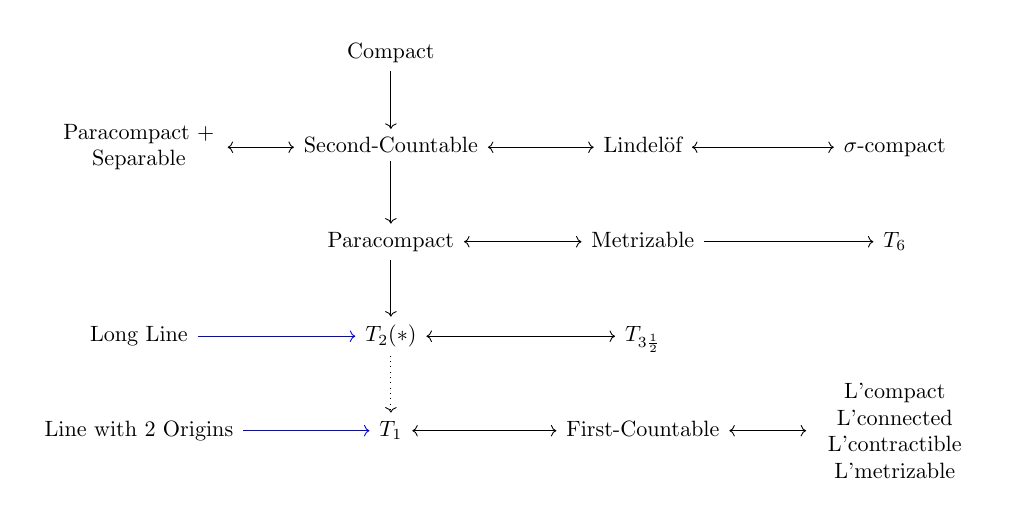
\begin{tikzpicture}	
			\node[scale=.8] (a) at (0,0){
				\begin{tikzcd}[anchor=center,
					column sep={4.0cm,between origins},
					row sep={1.5cm,between origins}
					]
					%%%%%%%%%%%%%%%
					&\text{Compact}\ar[d]&&\\
					%%%%%%%%%%%%%%%
					%\begin{aligned}\text{Paracompact} \\ \text{+ Separable}\end{aligned}
					\parbox{2.5cm}{\centering Paracompact + Separable}
					\ar[r,leftrightarrow]
					&\text{Second-Countable}\ar[d]&\text{Lindelöf}\ar[l,leftrightarrow]&\sigma\text{-compact}\ar[l,leftrightarrow]\\
					%%%%%%%%%%%%%%%
					&\text{Paracompact}\ar[d]&\text{Metrizable}\ar[l,leftrightarrow]&T_6\ar[from=l]\\
					%%%%%%%%%%%%%%%
					\text{Long Line}\ar[r,blue]&T_2 (*) \ar[d,dotted]& T_{3\frac{1}{2}}\ar[l,leftrightarrow] \\
					%%%%%%%%%%%%%%%
					\text{Line with 2 Origins}\ar[r,blue]&T_1\ar[r,leftrightarrow]&\text{First-Countable}\ar[r,leftrightarrow]&
					\parbox{2.5cm}{\centering L'compact L'connected L'contractible L'metrizable}
				\end{tikzcd}
			};
		\end{tikzpicture}
		\caption{Hierarchy of manifolds. Any manifold above $T_2$ assumes $T_2$, whereas those below only assumes locally Euclidean.
			A Property starting with ``L'' indicates it is local.
		}
		\label{fig:manifold_hierarchy}
	\end{figure}

	\paragraph{Examples}
	
	\subsection{Lie groups: definitions}
	
	\subsection{Examples of Lie groups}
	
	\subsection{Two constructions}
\end{document}
